\PassOptionsToPackage{unicode=true}{hyperref} % options for packages loaded elsewhere
\PassOptionsToPackage{hyphens}{url}
%
\documentclass[]{book}
\usepackage{lmodern}
\usepackage{amssymb,amsmath}
\usepackage{ifxetex,ifluatex}
\usepackage{fixltx2e} % provides \textsubscript
\ifnum 0\ifxetex 1\fi\ifluatex 1\fi=0 % if pdftex
  \usepackage[T1]{fontenc}
  \usepackage[utf8]{inputenc}
  \usepackage{textcomp} % provides euro and other symbols
\else % if luatex or xelatex
  \usepackage{unicode-math}
  \defaultfontfeatures{Ligatures=TeX,Scale=MatchLowercase}
\fi
% use upquote if available, for straight quotes in verbatim environments
\IfFileExists{upquote.sty}{\usepackage{upquote}}{}
% use microtype if available
\IfFileExists{microtype.sty}{%
\usepackage[]{microtype}
\UseMicrotypeSet[protrusion]{basicmath} % disable protrusion for tt fonts
}{}
\IfFileExists{parskip.sty}{%
\usepackage{parskip}
}{% else
\setlength{\parindent}{0pt}
\setlength{\parskip}{6pt plus 2pt minus 1pt}
}
\usepackage{hyperref}
\hypersetup{
            pdftitle={Multivariate Statistics},
            pdfauthor={Prof.~Richard Wilkinson},
            pdfborder={0 0 0},
            breaklinks=true}
\urlstyle{same}  % don't use monospace font for urls
\usepackage{color}
\usepackage{fancyvrb}
\newcommand{\VerbBar}{|}
\newcommand{\VERB}{\Verb[commandchars=\\\{\}]}
\DefineVerbatimEnvironment{Highlighting}{Verbatim}{commandchars=\\\{\}}
% Add ',fontsize=\small' for more characters per line
\usepackage{framed}
\definecolor{shadecolor}{RGB}{248,248,248}
\newenvironment{Shaded}{\begin{snugshade}}{\end{snugshade}}
\newcommand{\AlertTok}[1]{\textcolor[rgb]{0.94,0.16,0.16}{#1}}
\newcommand{\AnnotationTok}[1]{\textcolor[rgb]{0.56,0.35,0.01}{\textbf{\textit{#1}}}}
\newcommand{\AttributeTok}[1]{\textcolor[rgb]{0.77,0.63,0.00}{#1}}
\newcommand{\BaseNTok}[1]{\textcolor[rgb]{0.00,0.00,0.81}{#1}}
\newcommand{\BuiltInTok}[1]{#1}
\newcommand{\CharTok}[1]{\textcolor[rgb]{0.31,0.60,0.02}{#1}}
\newcommand{\CommentTok}[1]{\textcolor[rgb]{0.56,0.35,0.01}{\textit{#1}}}
\newcommand{\CommentVarTok}[1]{\textcolor[rgb]{0.56,0.35,0.01}{\textbf{\textit{#1}}}}
\newcommand{\ConstantTok}[1]{\textcolor[rgb]{0.00,0.00,0.00}{#1}}
\newcommand{\ControlFlowTok}[1]{\textcolor[rgb]{0.13,0.29,0.53}{\textbf{#1}}}
\newcommand{\DataTypeTok}[1]{\textcolor[rgb]{0.13,0.29,0.53}{#1}}
\newcommand{\DecValTok}[1]{\textcolor[rgb]{0.00,0.00,0.81}{#1}}
\newcommand{\DocumentationTok}[1]{\textcolor[rgb]{0.56,0.35,0.01}{\textbf{\textit{#1}}}}
\newcommand{\ErrorTok}[1]{\textcolor[rgb]{0.64,0.00,0.00}{\textbf{#1}}}
\newcommand{\ExtensionTok}[1]{#1}
\newcommand{\FloatTok}[1]{\textcolor[rgb]{0.00,0.00,0.81}{#1}}
\newcommand{\FunctionTok}[1]{\textcolor[rgb]{0.00,0.00,0.00}{#1}}
\newcommand{\ImportTok}[1]{#1}
\newcommand{\InformationTok}[1]{\textcolor[rgb]{0.56,0.35,0.01}{\textbf{\textit{#1}}}}
\newcommand{\KeywordTok}[1]{\textcolor[rgb]{0.13,0.29,0.53}{\textbf{#1}}}
\newcommand{\NormalTok}[1]{#1}
\newcommand{\OperatorTok}[1]{\textcolor[rgb]{0.81,0.36,0.00}{\textbf{#1}}}
\newcommand{\OtherTok}[1]{\textcolor[rgb]{0.56,0.35,0.01}{#1}}
\newcommand{\PreprocessorTok}[1]{\textcolor[rgb]{0.56,0.35,0.01}{\textit{#1}}}
\newcommand{\RegionMarkerTok}[1]{#1}
\newcommand{\SpecialCharTok}[1]{\textcolor[rgb]{0.00,0.00,0.00}{#1}}
\newcommand{\SpecialStringTok}[1]{\textcolor[rgb]{0.31,0.60,0.02}{#1}}
\newcommand{\StringTok}[1]{\textcolor[rgb]{0.31,0.60,0.02}{#1}}
\newcommand{\VariableTok}[1]{\textcolor[rgb]{0.00,0.00,0.00}{#1}}
\newcommand{\VerbatimStringTok}[1]{\textcolor[rgb]{0.31,0.60,0.02}{#1}}
\newcommand{\WarningTok}[1]{\textcolor[rgb]{0.56,0.35,0.01}{\textbf{\textit{#1}}}}
\usepackage{longtable,booktabs}
% Fix footnotes in tables (requires footnote package)
\IfFileExists{footnote.sty}{\usepackage{footnote}\makesavenoteenv{longtable}}{}
\usepackage{graphicx,grffile}
\makeatletter
\def\maxwidth{\ifdim\Gin@nat@width>\linewidth\linewidth\else\Gin@nat@width\fi}
\def\maxheight{\ifdim\Gin@nat@height>\textheight\textheight\else\Gin@nat@height\fi}
\makeatother
% Scale images if necessary, so that they will not overflow the page
% margins by default, and it is still possible to overwrite the defaults
% using explicit options in \includegraphics[width, height, ...]{}
\setkeys{Gin}{width=\maxwidth,height=\maxheight,keepaspectratio}
\setlength{\emergencystretch}{3em}  % prevent overfull lines
\providecommand{\tightlist}{%
  \setlength{\itemsep}{0pt}\setlength{\parskip}{0pt}}
\setcounter{secnumdepth}{5}
% Redefines (sub)paragraphs to behave more like sections
\ifx\paragraph\undefined\else
\let\oldparagraph\paragraph
\renewcommand{\paragraph}[1]{\oldparagraph{#1}\mbox{}}
\fi
\ifx\subparagraph\undefined\else
\let\oldsubparagraph\subparagraph
\renewcommand{\subparagraph}[1]{\oldsubparagraph{#1}\mbox{}}
\fi

% set default figure placement to htbp
\makeatletter
\def\fps@figure{htbp}
\makeatother

\usepackage{booktabs}
\usepackage{amsthm}
\DeclareMathOperator*{\argmin}{argmin}
\newcommand{\test}{\mathrm{test}}
\usepackage{titling}
\pretitle{\begin{center} \includegraphics[width=2in,height=2in]{figs/UoN_Primary_Logo_RGB.png}\LARGE\\}
\posttitle{\end{center}}
\usepackage{booktabs}
\usepackage{longtable}
\usepackage{array}
\usepackage{multirow}
\usepackage{wrapfig}
\usepackage{float}
\usepackage{colortbl}
\usepackage{pdflscape}
\usepackage{tabu}
\usepackage{threeparttable}
\usepackage{threeparttablex}
\usepackage[normalem]{ulem}
\usepackage{makecell}
\usepackage[]{natbib}
\bibliographystyle{apalike}

\title{Multivariate Statistics}
\author{Prof.~Richard Wilkinson}
\date{Spring 2021}

\usepackage{amsthm}
\newtheorem{theorem}{Theorem}[chapter]
\newtheorem{lemma}{Lemma}[chapter]
\newtheorem{corollary}{Corollary}[chapter]
\newtheorem{proposition}{Proposition}[chapter]
\newtheorem{conjecture}{Conjecture}[chapter]
\theoremstyle{definition}
\newtheorem{definition}{Definition}[chapter]
\theoremstyle{definition}
\newtheorem{example}{Example}[chapter]
\theoremstyle{definition}
\newtheorem{exercise}{Exercise}[chapter]
\theoremstyle{remark}
\newtheorem*{remark}{Remark}
\newtheorem*{solution}{Solution}
\begin{document}
\maketitle

{
\setcounter{tocdepth}{1}
\tableofcontents
}
\hypertarget{introduction}{%
\chapter*{Introduction}\label{introduction}}
\addcontentsline{toc}{chapter}{Introduction}

\newcommand{\tr}{\operatorname{tr}}
\newcommand{\indep}{\perp \!\!\! \perp}
\newcommand{\bY}{\boldsymbol Y}
\newcommand{\bx}{\boldsymbol x}
\newcommand{\bX}{\boldsymbol X}
\newcommand{\bH}{\boldsymbol H}
\newcommand{\by}{\boldsymbol y}
\newcommand{\bz}{\boldsymbol z}
\newcommand{\bS}{\boldsymbol S}
\newcommand{\bR}{\boldsymbol R}
\newcommand{\bF}{\boldsymbol F}
\newcommand{\bI}{\mathbf I}
\newcommand{\bmu}{\boldsymbol \mu}
\newcommand{\bSigma}{\boldsymbol \Sigma}
\newcommand{\bLambda}{\boldsymbol \Lambda}
\newcommand{\bgamma}{\boldsymbol \gamma}
\newcommand{\btheta}{\boldsymbol \theta}
\newcommand{\bdelta}{\boldsymbol \delta}
\newcommand{\bbeta}{\boldsymbol \beta}
\newcommand{\blambda}{\boldsymbol \lambda}
\newcommand{\bA}{\boldsymbol A}
\newcommand{\bB}{\boldsymbol B}
\newcommand{\bC}{\boldsymbol C}
\newcommand{\bD}{\boldsymbol D}
\newcommand{\bE}{\boldsymbol E}
\newcommand{\bG}{\boldsymbol G}
\newcommand{\bM}{\boldsymbol M}
\newcommand{\bP}{\boldsymbol P}
\newcommand{\bQ}{\boldsymbol Q}
\newcommand{\bT}{\boldsymbol T}
\newcommand{\bV}{\boldsymbol V}
\newcommand{\bU}{\boldsymbol U}
\newcommand{\bW}{\boldsymbol W}
\newcommand{\bZ}{\boldsymbol Z}

\newcommand{\ba}{\boldsymbol a}
\newcommand{\bb}{\boldsymbol b}
\newcommand{\bc}{\boldsymbol c}
\newcommand{\bd}{\boldsymbol d}
\newcommand{\be}{\boldsymbol e}
\newcommand{\bh}{\boldsymbol h}
\newcommand{\bk}{\boldsymbol k}
\newcommand{\bp}{\boldsymbol p}
\newcommand{\bq}{\boldsymbol q}
\newcommand{\br}{\boldsymbol r}
\newcommand{\bt}{{\boldsymbol t}}
\newcommand{\bu}{\boldsymbol u}
\newcommand{\bv}{\boldsymbol v}
\newcommand{\bw}{\boldsymbol w}
\newcommand{\bzero}{\boldsymbol 0}
\newcommand{\mR}{\mathbb R}
\newcommand{\cR}{\mathcal R}

\newcommand{\bs}{\boldsymbol}
\newcommand{\ds}{\displaystyle}
\newcommand{\tdiag}{\text{diag}}
\newcommand{\ttr}{\text{tr}}
\newcommand{\tmin}{\text{min}}
\newcommand{\tmax}{\text{max}}
\newcommand{\tdet}{\text{det}}

\newcommand{\tcov}{\text{cov}}
\newcommand{\texp}{\text{exp}}
\newcommand{\lb}{\left(}
\newcommand{\rb}{\right)}
\newcommand{\lsb}{\left[}
\newcommand{\rsb}{\right]}
\newcommand{\BE}{{\mathbb{E}}}
\newcommand{\cov}{{\mathbb{C}\operatorname{ov}}}
\newcommand{\var}{{\mathbb{V}\operatorname{ar}}}

\textbf{Warning:} these lecture notes are still in preparation. Chapters 1-4 have been finished. Chapters 5-6 are being worked on. Later chapters will appear once a reasonable draft is available.

This module is concerned with the analysis of multivariate data, in which the response is a vector of random variables rather than a single random variable.

Part I of the module describes some basic concepts in Multivariate Analysis and then recaps and introduces some key ideas needed from linear algebra.
Chapter \ref{stat-prelim} defines notation, introduces some datasets, and discusses exploratory data analysis. Chapter \ref{linalg-prelim} provides a recap on some matrix algebra. Much of this will be familiar to you, but if not, we take the time to introduce the key mathematical concepts that will be relied upon during the module. Chapter \ref{linalg-decomp} introduces matrix decompositions. We start with the spectral decomposition of square symmetric matrices (which you will have studied previously), and then introduce the singular value decomposition (SVD). The SVD is one of the most important concepts in this module, and is the key linear algebra technique behind many of the methods we will study.

A theme running through the module is that of dimension reduction. In Part II we consider three types of dimension reduction: Principal Components Analysis (in Chapter \ref{pca}),
whose purpose is to identify the main modes of variation in a multivariate dataset; Canonical Correlation Analysis (Chapter \ref{cca}), whose purpose is to describe the association between two sets of variables; and Multidimensional Scaling (Chapter \ref{mds}), in which the starting point is a set of pairwise distances, suitably defined, between the objects under study.

In Part III, we focus on methods of inference for multivariate data whose distribution is multivariate normal.

Finally, in Part IV, we focus on different methods of classification, i.e.~allocating the observations in a sample to different subsets (or groups).

If you find any typos or mistakes, please email me at \texttt{r.d.wilkinson@nottingham.ac.uk} The notes have been significantly rewritten this year in order to adapt them for remote learning, and I am keen to fix as many of the mistakes as I can!

\hypertarget{part-i-prerequisites}{%
\chapter*{PART I: Prerequisites}\label{part-i-prerequisites}}
\addcontentsline{toc}{chapter}{PART I: Prerequisites}

Much of modern multivariate statistics (and machine learning) relies upon linear algebra. Consequently, we will spend some time reminding you of the basics of linear algebra (vector spaces, matrices etc), and introducing a few additional concepts that you may not have seen before. It is worth spending time familiarizing yourself with these ideas, as we will rely heavily upon this material in later chapters.

In Chapter \ref{stat-prelim} we explain what we mean by multivariate analysis and give some examples of multivariate data. We introduce basic definitions and concepts such as the sample covariance matrix, the sample correlation matrix and describe some simple exploratory data analysis techniques.

In Chapter \ref{linalg-prelim} we summarise the definitions, ideas and results from matrix algebra that will be needed later in the module, most of which will be familiar to you. In particular, we will introduce vector spaces and the concept of a basis for a vector space, discuss the column, row and null space of matrices, and discuss inner product spaces and projections. We also define the centering matrix.

In Chapter \ref{linalg-decomp} we recap the eigen or spectral decomposition of square symmetric matrices, and introduce the singular value decomposition (SVD) which generalises the concept of eigenvalues for non-square matrices. We will rely upon this material inlater chapters.

\renewcommand{\bY}{\boldsymbol Y}
\renewcommand{\bx}{\boldsymbol x}
\renewcommand{\bX}{\boldsymbol X}
\renewcommand{\bH}{\boldsymbol H}
\renewcommand{\by}{\boldsymbol y}
\renewcommand{\bz}{\boldsymbol z}
\renewcommand{\bS}{\boldsymbol S}
\renewcommand{\bR}{\boldsymbol R}
\renewcommand{\bmu}{\boldsymbol \mu}
\renewcommand{\bSigma}{\boldsymbol \Sigma}
\renewcommand{\bLambda}{\boldsymbol \Lambda}
\renewcommand{\bgamma}{\boldsymbol \gamma}
\renewcommand{\blambda}{\boldsymbol \lambda}
\renewcommand{\bA}{\boldsymbol A}
\renewcommand{\bB}{\boldsymbol B}
\renewcommand{\bD}{\boldsymbol D}
\renewcommand{\bM}{\boldsymbol M}
\renewcommand{\bP}{\boldsymbol P}
\renewcommand{\bQ}{\boldsymbol Q}
\renewcommand{\bT}{\boldsymbol T}
\renewcommand{\bW}{\boldsymbol W}
\renewcommand{\ba}{\boldsymbol a}
\renewcommand{\bb}{\boldsymbol b}
\renewcommand{\bc}{\boldsymbol c}
\renewcommand{\bd}{\boldsymbol d}
\renewcommand{\bh}{\boldsymbol h}
\renewcommand{\bp}{\boldsymbol p}
\renewcommand{\bq}{\boldsymbol q}
\renewcommand{\bu}{\boldsymbol u}
\renewcommand{\bzero}{\boldsymbol 0}
\renewcommand{\mR}{\mathbb R}
\renewcommand{\cR}{\mathcal R}

\renewcommand{\bs}{\boldsymbol}
\renewcommand{\ds}{\displaystyle}
\renewcommand{\tdiag}{\text{diag}}
\renewcommand{\ttr}{\text{tr}}
\renewcommand{\tmin}{\text{min}}
\renewcommand{\tmax}{\text{max}}
\renewcommand{\tdet}{\text{det}}

\renewcommand{\tcov}{\text{cov}}
\renewcommand{\texp}{\text{exp}}
\renewcommand{\lb}{\left(}
\renewcommand{\rb}{\right)}
\renewcommand{\lsb}{\left[}
\renewcommand{\rsb}{\right]}

\hypertarget{stat-prelim}{%
\chapter{Statistical Preliminaries}\label{stat-prelim}}

In this chapter we will define some notation, and recap some basic statistical properties and results.

There are recorded videos for the following topics in this chapter:

\begin{itemize}
\tightlist
\item
  \href{https://mediaspace.nottingham.ac.uk/media/Notation+and+Datasets/1_p2nas9i4}{Notation and datasets}
\item
  \href{https://mediaspace.nottingham.ac.uk/media/Exploratory+data+analysis/1_seh9o28a}{Exploratory data analysis}
\item
  \href{https://mediaspace.nottingham.ac.uk/media/Random+Vectors/1_fpq4r9wh}{Random vectors}
\end{itemize}

\hypertarget{notation}{%
\section{Notation}\label{notation}}

We will think of datasets as consisting of measurements of \(p\) different \textbf{variables} for \(n\) different \textbf{cases/subjects}. We organise the data into an \(n \times p\) \textbf{data matrix}.

\textbf{Multivariate analysis} (MVA) refers to data analysis methods where there are two or more \textbf{response} variables for each case (you are familiar with situations where there is more than one explanatory variable, e.g., multiple linear regression).

We shall often write the data matrix as \(\mathbf X\) (\(n \times p\)) where
\[
{\mathbf X}=\left[ \begin{array}{ccc}
- &\boldsymbol x_1^\top&-\\
- &\boldsymbol x_2^\top&-\\
- &..&-\\
- &\boldsymbol x_n^\top&-
\end{array}\right ]
\]
The vectors \(\boldsymbol x_1, \ldots , \boldsymbol x_n \in \mathbb{R}^p\) are the observation vectors for each of the \(n\) subjects.

\begin{itemize}
\tightlist
\item
  The \(n\) \emph{rows} of \(\mathbf X\) are \(\boldsymbol x_1^\top, \ldots , \boldsymbol x_n^\top\) - each row contains the \(p\) observations on a single subject.
\item
  The \(p\) columns of \(\mathbf X\) correspond to the \(p\) variables being measured, i.e., they contain the measurements of the same variable across all \(n\) subjects.
\end{itemize}

\textbf{Important remark on notation:} Throughout the module we shall use

\begin{itemize}
\tightlist
\item
  non-bold letters, whether upper or lower case, to indicate scalar (i.e.~real-valued) quantities, e.g., \(x, y\)
\item
  lower-case letters in bold to signify column vectors, e.g., \(\boldsymbol x, \boldsymbol y\)
\item
  upper case letters in bold to signify matrices, e.g., \(\boldsymbol X, \boldsymbol Y\).
\end{itemize}

This convention for bold letters will also apply to random quantities. So, in particular, for a random vector we always use (bold) lower case, and for a random matrix we always use bold upper-case, regardless of whether we are referring to (i) the unobserved random quantity or (ii) its observed value. It should always be clear from the context which of these two interpretations (i) or (ii) is appropriate.

\hypertarget{example-datasets}{%
\subsection{Example datasets}\label{example-datasets}}

\begin{example}
\protect\hypertarget{exm:football}{}{\label{exm:football} }The football league table is an example of multivariate data. Here \(W =\) number of wins, \(D =\) number of draws, \(F =\) number of goals scored and \(A =\) number of goals conceded for four teams.
In this example we have \(p=4\) variables \((W, D, F, A)^\top\) measured on \(n=4\) cases (teams).
\end{example}

\begin{table}[H]
\centering
\begin{tabular}{lrrrr}
\toprule
Team & W & D & F & A\\
\midrule
USA & 1 & 2 & 4 & 3\\
England & 1 & 2 & 2 & 1\\
Slovenia & 1 & 1 & 3 & 3\\
Algeria & 0 & 1 & 0 & 2\\
\bottomrule
\end{tabular}
\end{table}

The data vector for the USA is
\[x_1^\top=(1,2,4,3)\]

\begin{example}
\protect\hypertarget{exm:exam}{}{\label{exm:exam} }Exam marks for a set of \(n\) students where \(P =\) mark in probability and \(S =\) mark in statistics.
Let \(x_{ij}\) denote the \(j\)th variable measured on the \(i\)th subject.
\end{example}

\begin{table}[H]
\centering
\begin{tabular}{lll}
\toprule
Student & P & S\\
\midrule
1 & $x_{11}$ & $x_{12}$\\
2 & $x_{21}$ & $x_{22}$\\
$\vdots$ & $\vdots$ & $\vdots$\\
n & $x_{n1}$ & $x_{n2}$\\
\bottomrule
\end{tabular}
\end{table}

\begin{example}
\protect\hypertarget{exm:iris}{}{\label{exm:iris} }The \texttt{iris} dataset is a famous set of measurements collected on the sepal length and width, and the petal length and width, of 50 flowers for each of 3 species of iris (setosa, versicolor, and virginica). The dataset is built into R (try typing \texttt{iris} in R) and is often used to demonstrate multivariate statistical methods. For these data, \(p=5\), and \(n=150\).
\end{example}

\begin{table}[H]
\centering
\begin{tabular}{rrrrl}
\toprule
Sepal.Length & Sepal.Width & Petal.Length & Petal.Width & Species\\
\midrule
5.1 & 3.5 & 1.4 & 0.2 & setosa\\
4.9 & 3.0 & 1.4 & 0.2 & setosa\\
4.7 & 3.2 & 1.3 & 0.2 & setosa\\
7.0 & 3.2 & 4.7 & 1.4 & versicolor\\
6.4 & 3.2 & 4.5 & 1.5 & versicolor\\
\addlinespace
6.9 & 3.1 & 4.9 & 1.5 & versicolor\\
6.3 & 3.3 & 6.0 & 2.5 & virginica\\
5.8 & 2.7 & 5.1 & 1.9 & virginica\\
7.1 & 3.0 & 5.9 & 2.1 & virginica\\
\bottomrule
\end{tabular}
\end{table}

\begin{example}
\protect\hypertarget{exm:mnist}{}{\label{exm:mnist} }The MNIST dataset is a collection of handwritten digits that is widely used in statistics and machine learning to test algorithms.
It contains 60,000 images of hand-written digits. Here are the first 12 images:

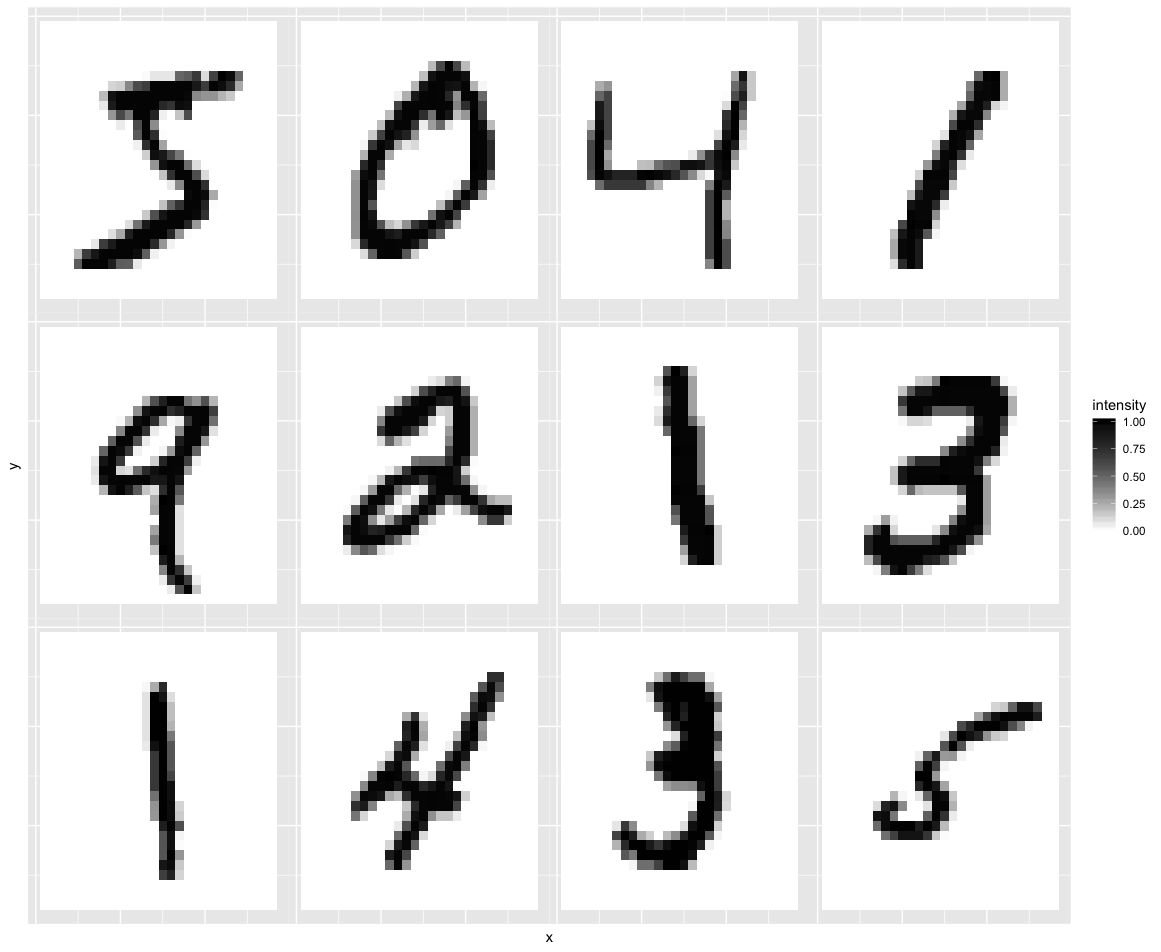
\includegraphics{MNIST2.png}

Each digit has been converted to a grid of \(28\times 28\) pixels, with a grayscale intensity level specified for each pixel. When we store these on a computer, we flatten each grid to a vector of length 784.
So for this dataset, \(n=60,000\) and \(p=784\). As an example of what the data look like, the intensities (times 100) for the first image above are shown in the plot below:

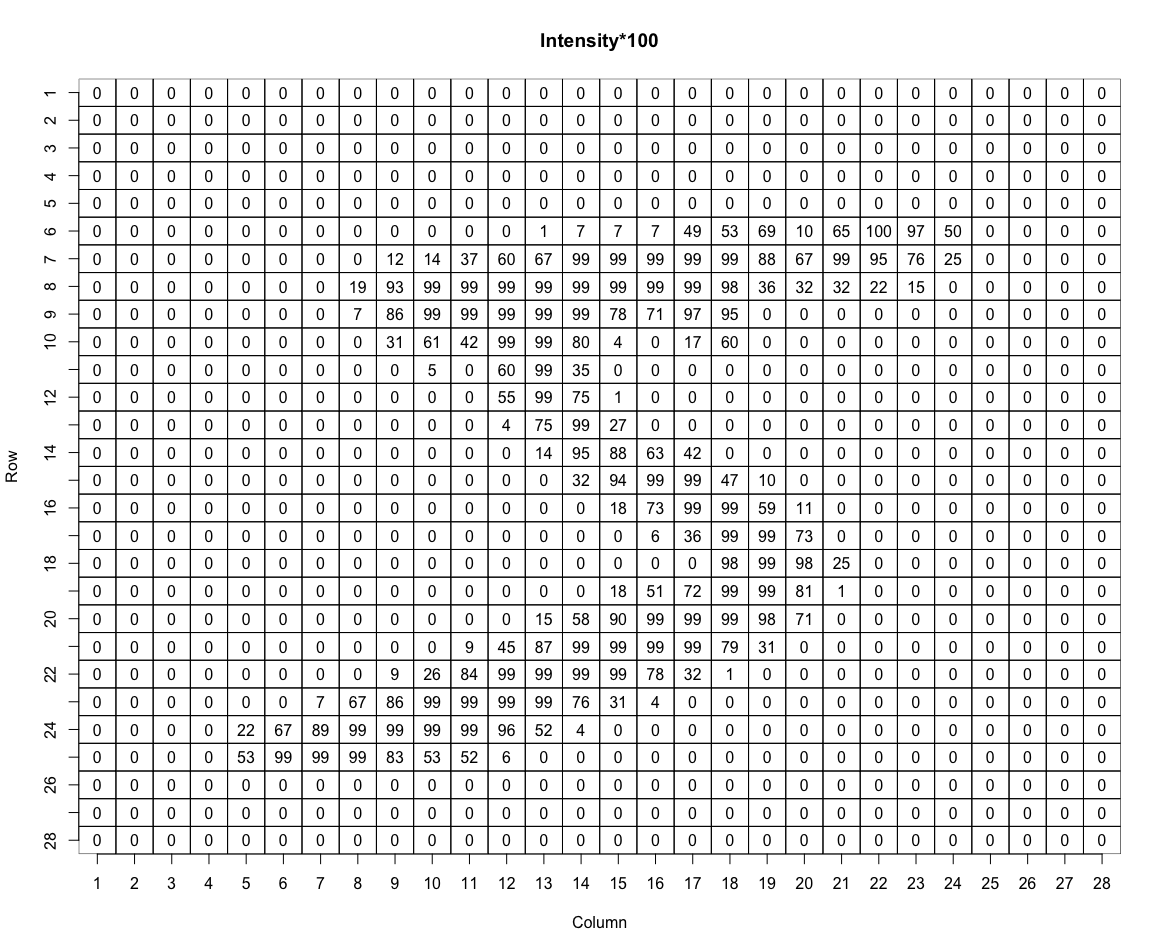
\includegraphics{MNIST3.png}
\end{example}

\hypertarget{aims-of-multivariate-data-analysis}{%
\subsection{Aims of multivariate data analysis}\label{aims-of-multivariate-data-analysis}}

The aim of multivariate statistical analysis is to answer questions such as:

\begin{itemize}
\tightlist
\item
  How can we visualise the data?
\item
  What is the joint distribution of marks?
\item
  Can we simplify the data? For example, we rank football teams using \(3W+D\) and we rank students by their average module mark. Is this fair? Can we reduce the dimension in a better way?
\item
  Can we use the data to discriminate, for example, between male and female students?
\item
  Are the different iris species different shapes?
\item
  Can we build a model to predict the intended digit from an image of someones handwriting? Or predict the species of iris from measurements of its sepal and petal?
\end{itemize}

We could just apply standard univariate techniques to each variable in turn, but this ignores possible dependencies between the variables which we must represent to draw valid conclusions.

\textbf{What is the difference between MVA and standard linear regression?}

\begin{itemize}
\tightlist
\item
  In standard linear regression we have a scalar response variable, \(y\) say, and a vector of covariates, \(\boldsymbol x\), say. The focus of interest is on how knowledge of \(\boldsymbol x\) influences the distribution of \(y\) (in particular, the mean of \(y\)). In contrast, in MVA the focus is a vector \(\boldsymbol y\), in which all the components of \(\boldsymbol y\) are viewed as responses rather than covariates, possibly with additional covariate information \(\boldsymbol x\). We will discuss this further in Chapter \ref{lm}.
\end{itemize}

\hypertarget{exploratory-data-analysis-eda}{%
\section{Exploratory data analysis (EDA)}\label{exploratory-data-analysis-eda}}

\begin{quote}
A picture is worth a thousand words
\end{quote}

\begin{figure}
\centering
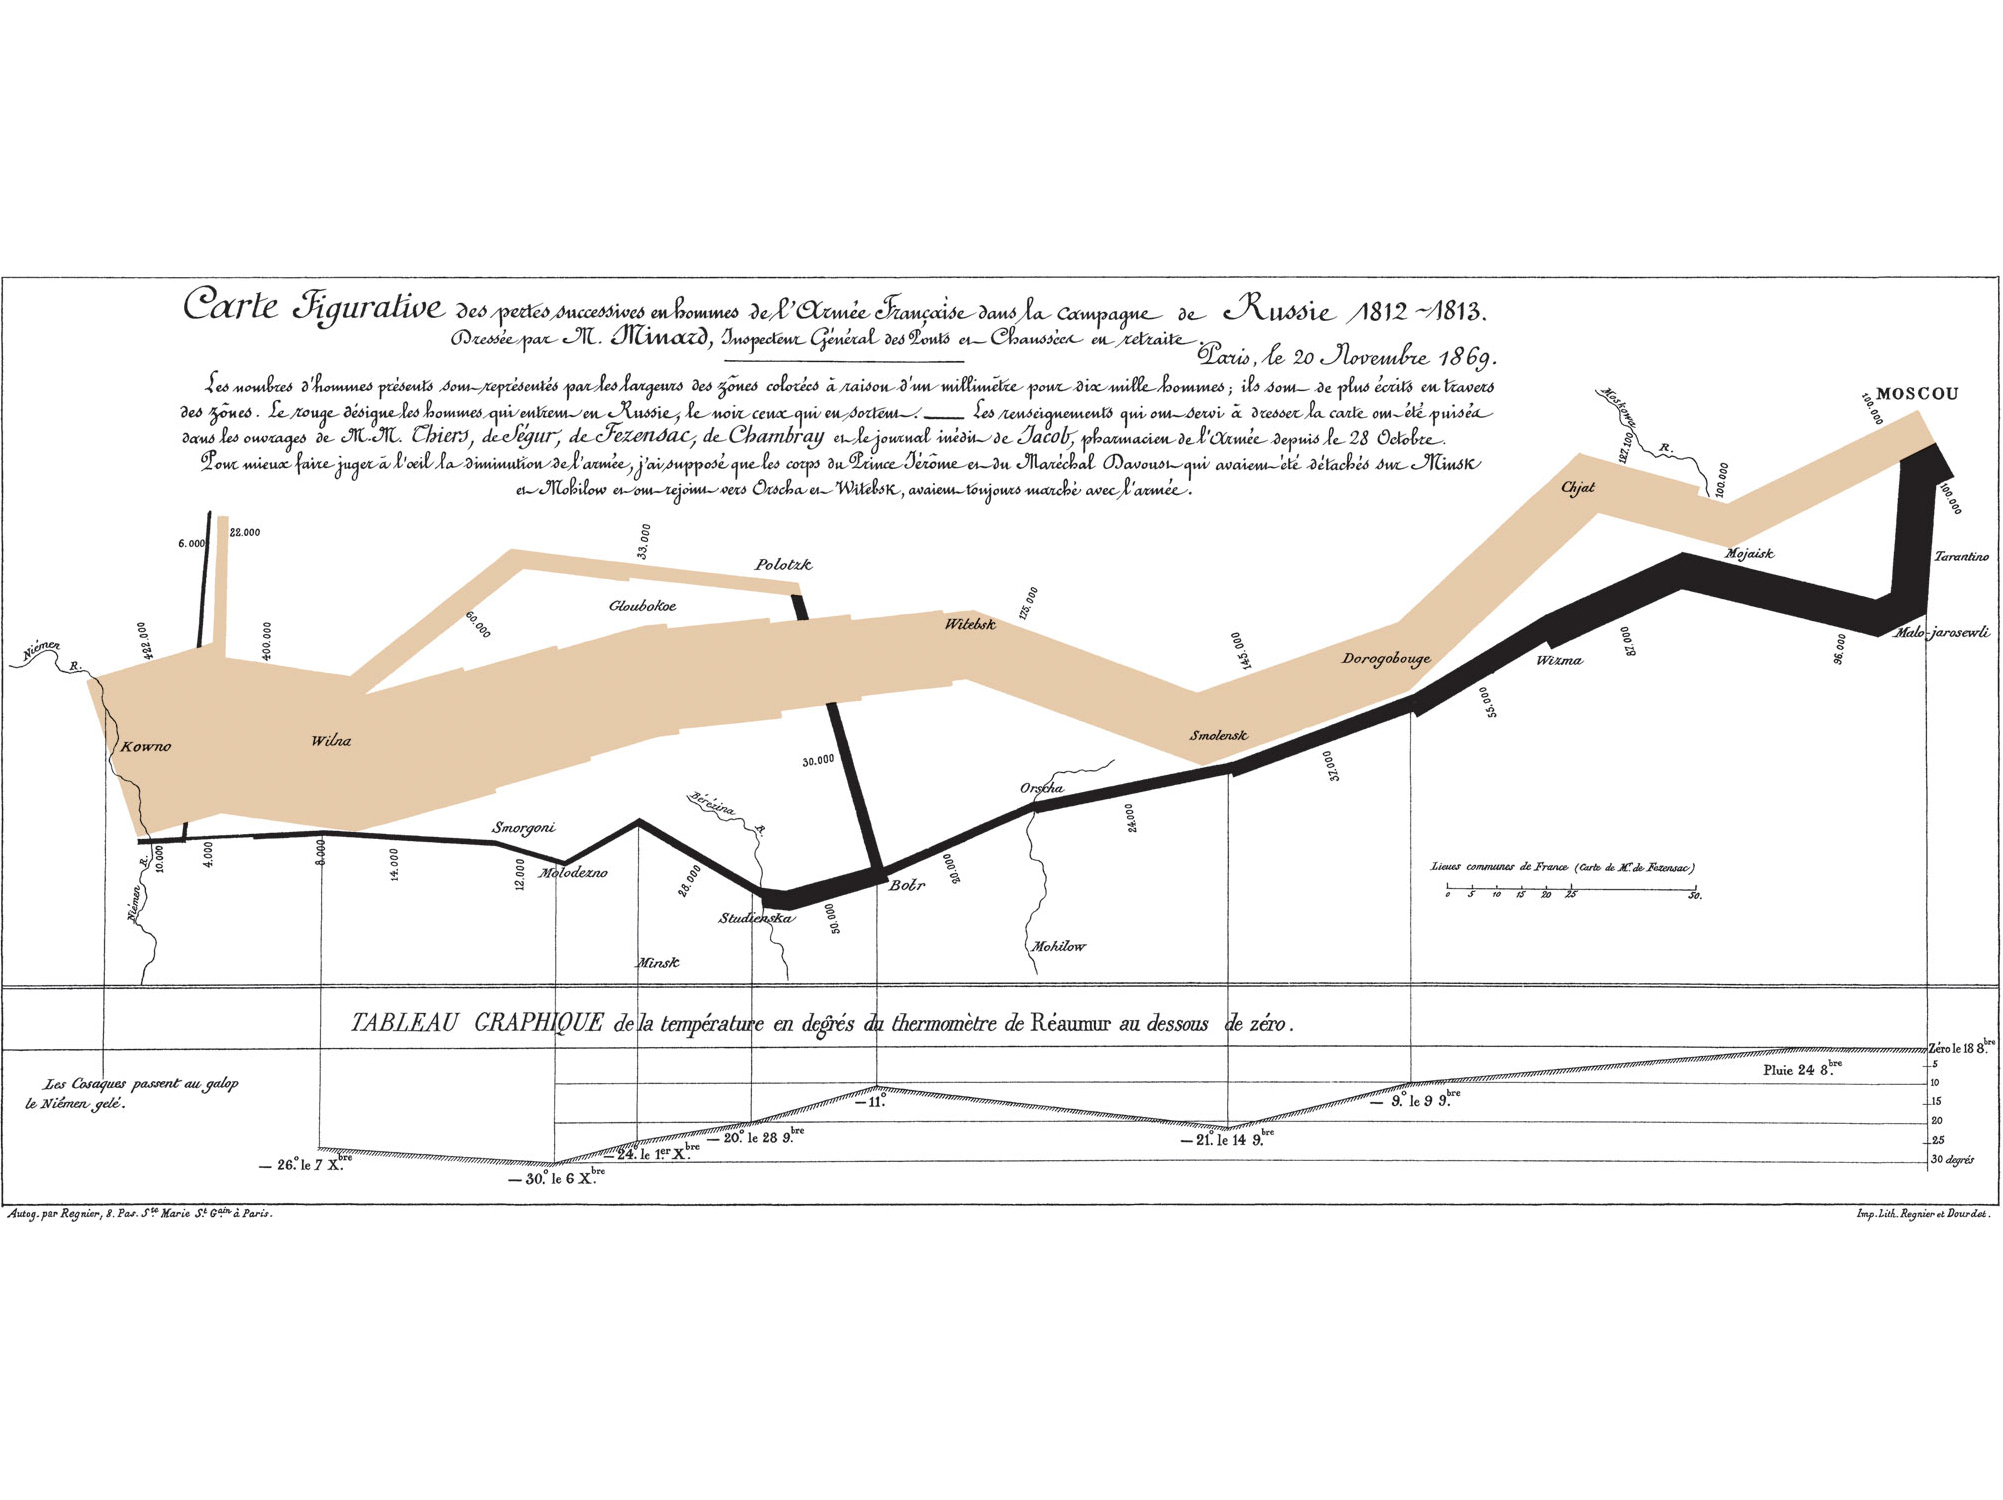
\includegraphics{figs/Minard.jpg}
\caption{\label{fig:unnamed-chunk-5}Charles Joseph Minard's famous map of Napoleon's 1812 invasion of Russian. It displays \href{https://en.wikipedia.org/wiki/Charles_Joseph_Minard\#The_map_of_Napoleon's_Russian_campaign}{six types of data in two dimensions}.}
\end{figure}

Before trying any form of statistical analysis, it is always a good idea to do some form of exploratory data analysis to understand the challenges presented by the data. As a minimum, this usually involves finding out whether each variable is continuous, discrete, or categorical, doing some basic visualization (plots), and perhaps computing a few summary statistics such as the mean and variance.

\hypertarget{data-visualization}{%
\subsection{Data visualization}\label{data-visualization}}

Visualising datasets before fitting any models can be extremely useful. It allows us to see obvious patterns and relationships,and may suggest a sensible form of analysis.
With multivariate data, finding the right kind of plot is not always simple, and many different approaches have been proposed.

When \(p=1\) or \(p=2\) we can simply draw histograms and scatter plots (respectively) to view the distribution. For \(p \geq 3\) the task is harder. One solution is a matrix of pair-wise scatter plots using the \texttt{pairs} command in R. The graph below shows the relationship between goals scored (F), goals against (A) and points (PT) for 20 teams during a recent Premiership season.

\begin{figure}
\centering
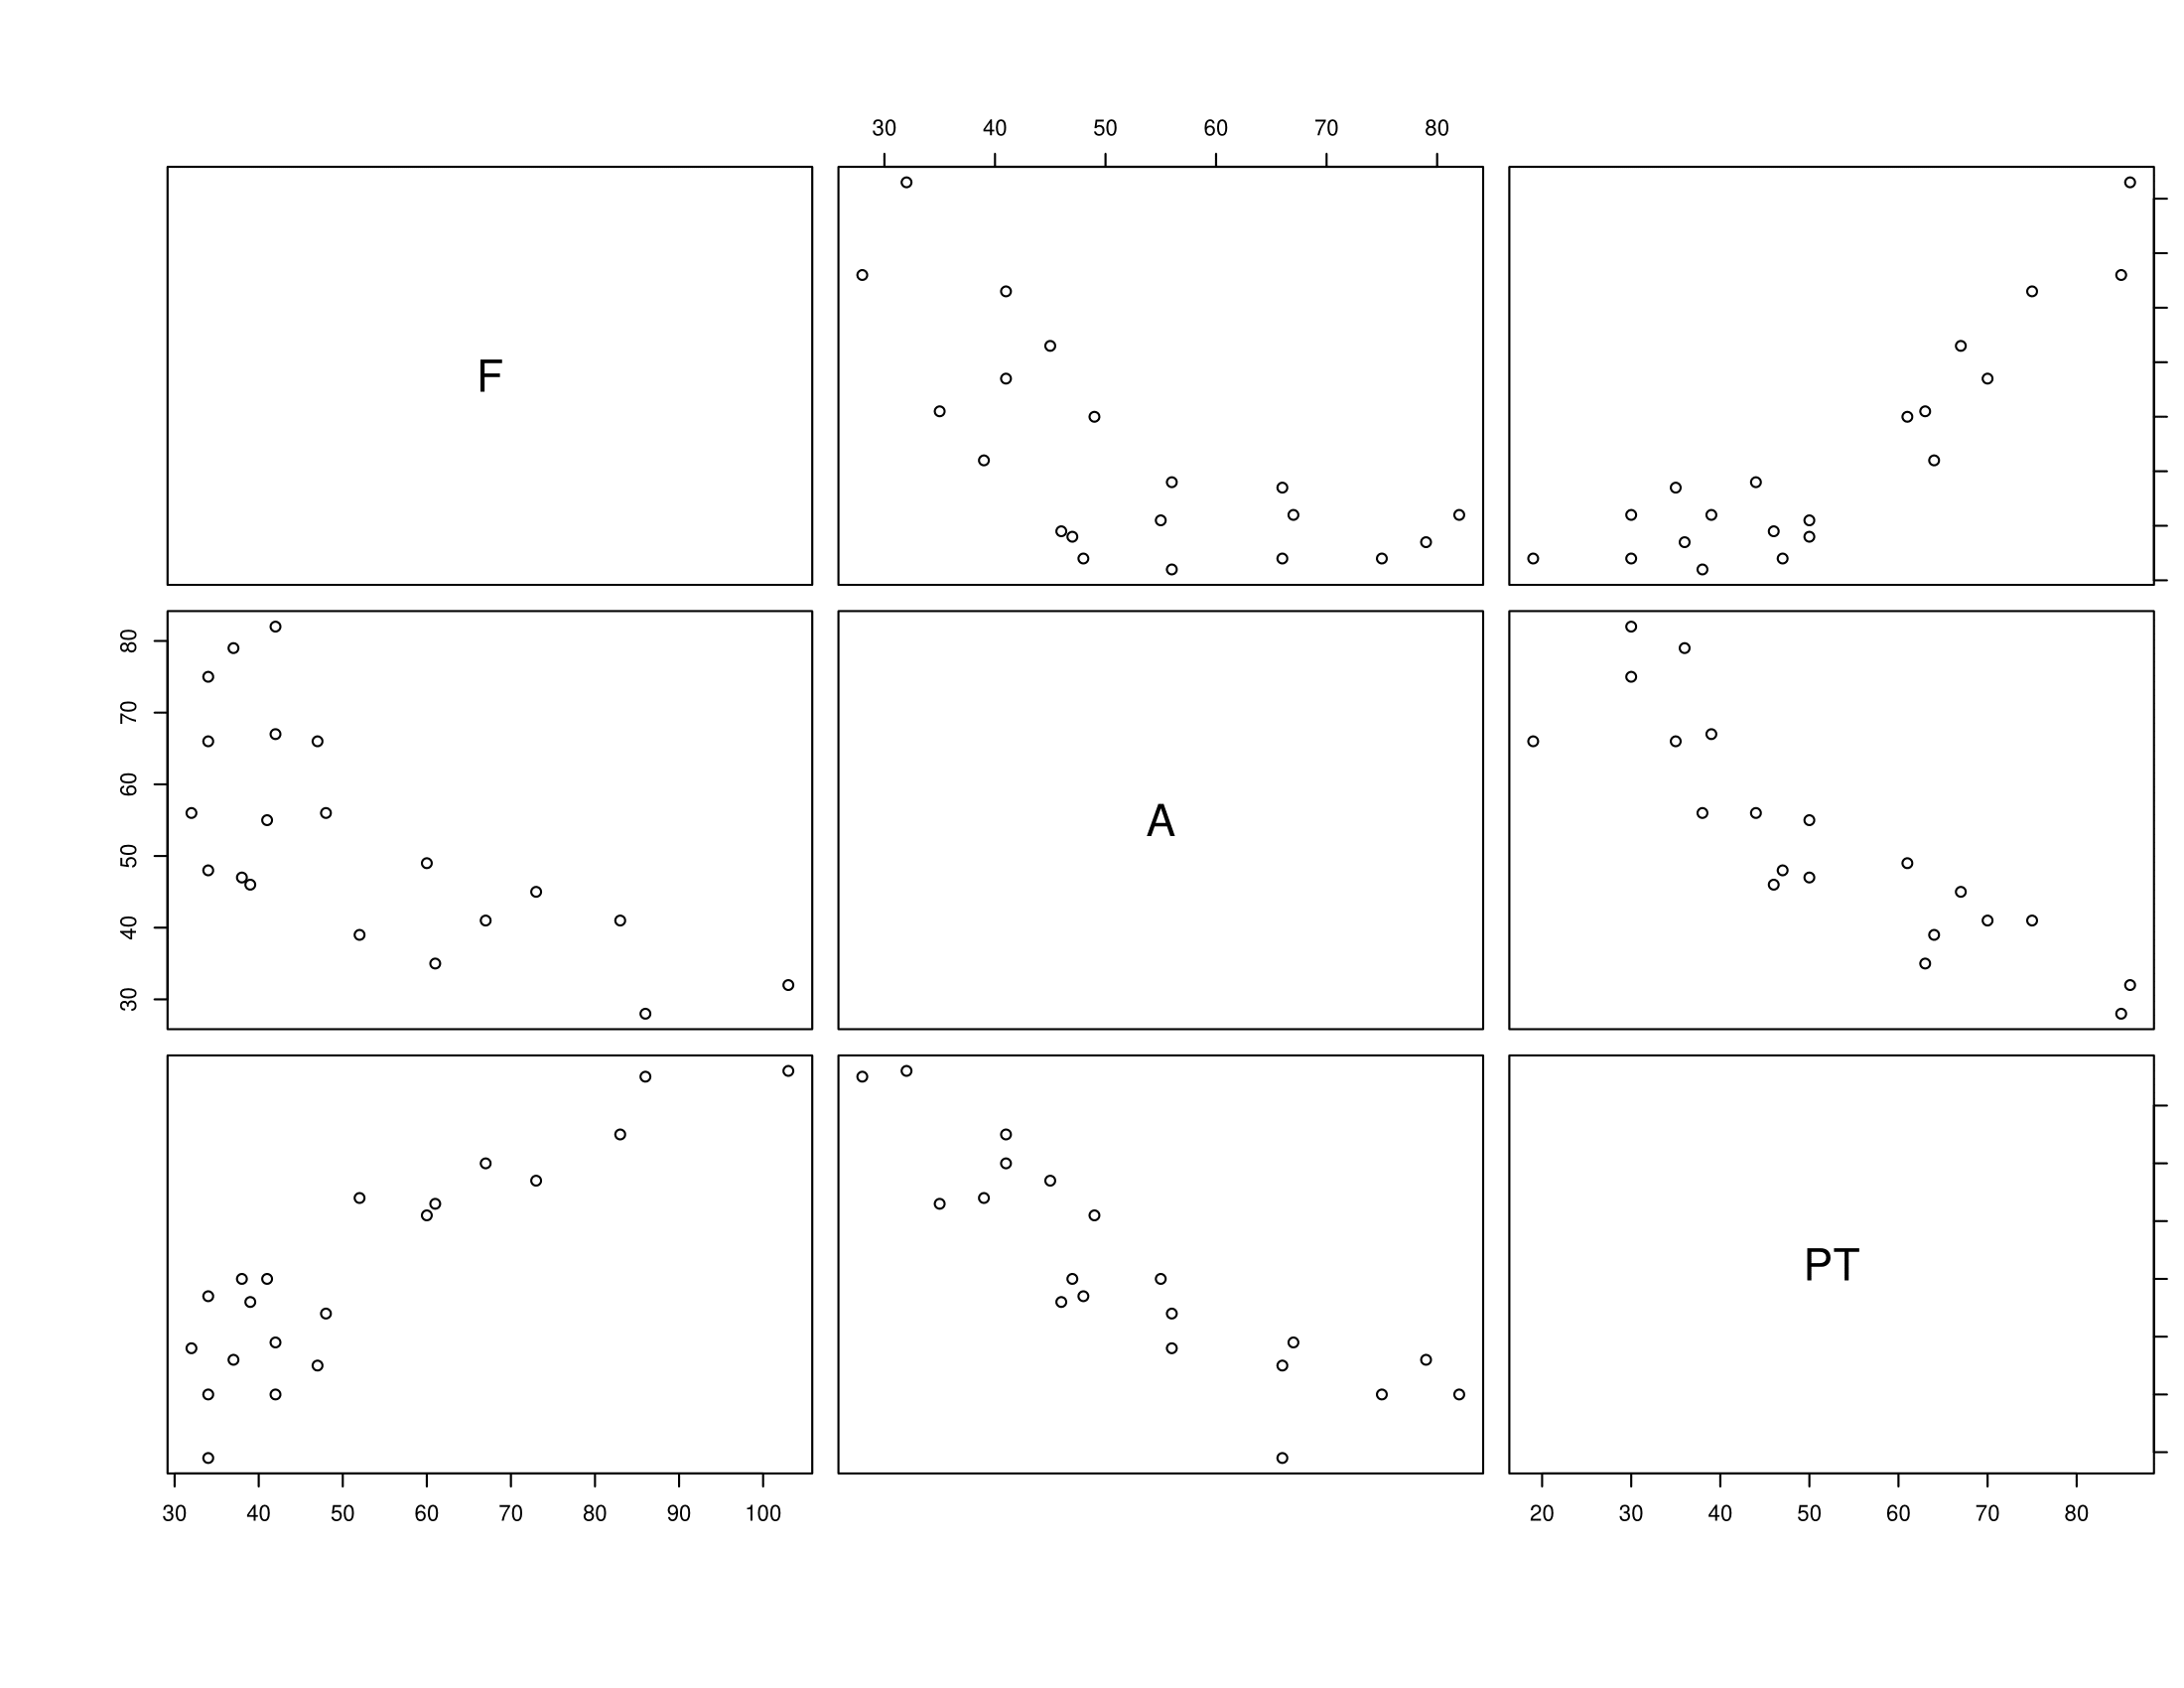
\includegraphics{figs/pairs.png}
\caption{\label{fig:unnamed-chunk-6}Scatter plots of goals for (F), goals against (A) and points (PT) for a recent Premier League Season}
\end{figure}

We can instantly see that points and goals scored are positively correlated, and that points and goals conceded (A) are negatively correlated (this is not a surprise of course).

R has a good basic plotting functionality. However, we will sometimes use packages that provide additional functionality. The first time you use a package you may need to install it. We can use \texttt{ggplot2} and \texttt{GGally} (which adds functionality to ggplot2) to add colour and detail to pairs plots. For example

\begin{Shaded}
\begin{Highlighting}[]
\KeywordTok{data}\NormalTok{(iris)}
\KeywordTok{library}\NormalTok{(ggplot2)}
\KeywordTok{library}\NormalTok{(GGally)}
\CommentTok{# pairs(iris) # - try the pairs command for comparison}
\KeywordTok{ggpairs}\NormalTok{(iris, }\DataTypeTok{columns=}\DecValTok{1}\OperatorTok{:}\DecValTok{4}\NormalTok{,  }\DataTypeTok{mapping=}\NormalTok{ggplot2}\OperatorTok{::}\KeywordTok{aes}\NormalTok{(}\DataTypeTok{colour =}\NormalTok{ Species),}
        \DataTypeTok{upper =} \KeywordTok{list}\NormalTok{(}\DataTypeTok{continuous =} \KeywordTok{wrap}\NormalTok{(}\StringTok{"cor"}\NormalTok{, }\DataTypeTok{size =} \DecValTok{3}\NormalTok{)))  }\CommentTok{# fix the font size}
\end{Highlighting}
\end{Shaded}

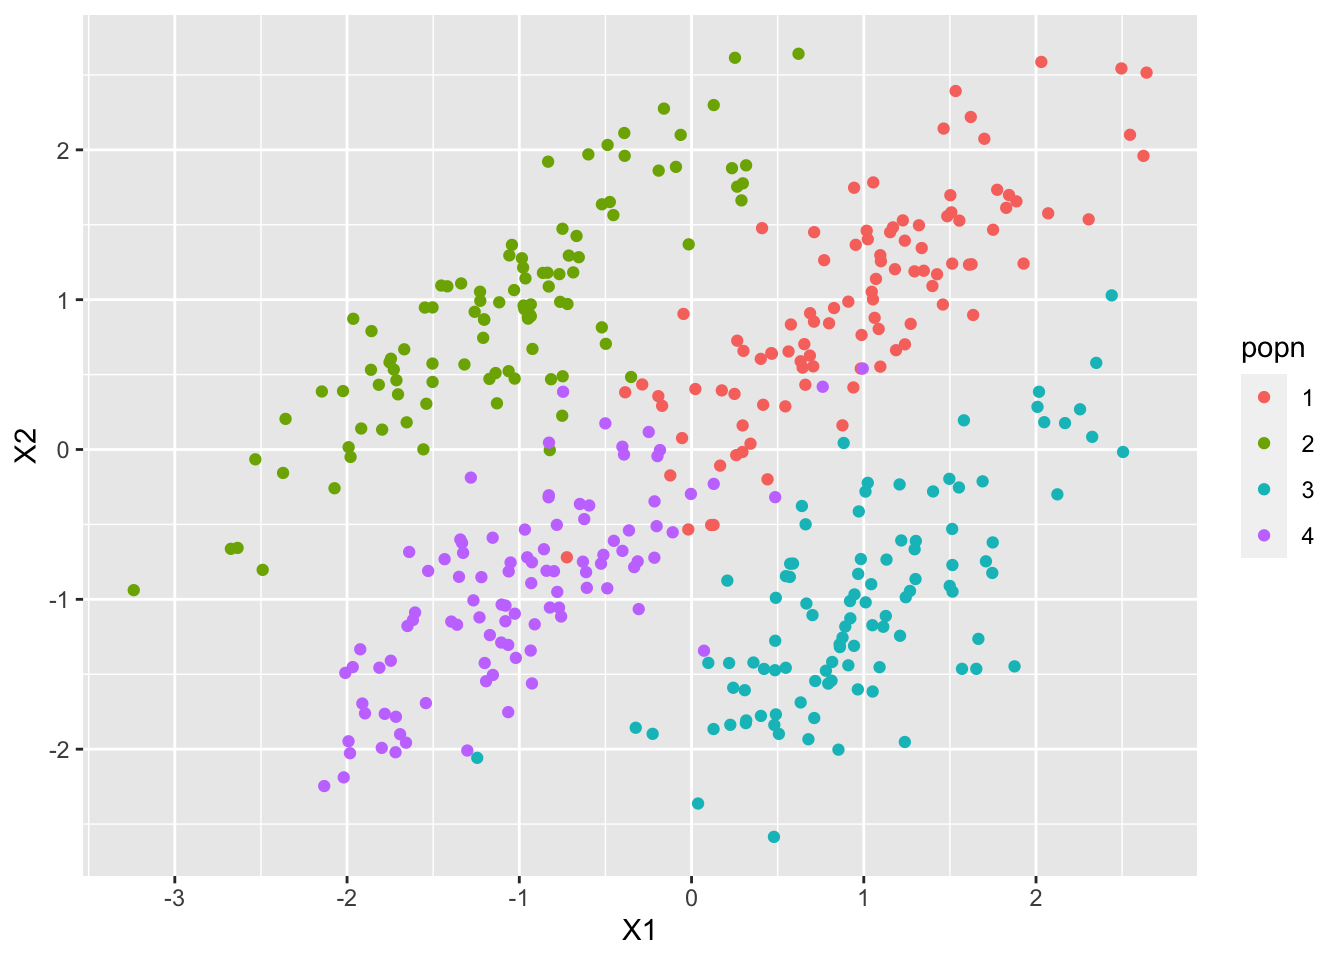
\includegraphics[width=1\linewidth]{01-statistical-prelim_files/figure-latex/unnamed-chunk-7-1}

This plot allows us to instantly see that there are clear differences between the three species of iris, at least when we look at the pairs plots. The benefit of adding colour in this case is that we can see the differences between the different species. Note how the sepal length and width are (weakly) negatively correlated across the entire dataset, but are positively correlated when we look at a single species at a time. We would have missed this information if we only used the \texttt{pairs} command (try it!).

Note that it is possible to miss key relationships when looking at \emph{marginals} plots such as these, as they only show two variables at a time. More complex relationships between three or more variables will not be visible. It is difficult visualize data in three or more dimensions. Many different types of plot have been proposed (e.g.~Google Chernoff faces). One approach is to use a \emph{parallel line} plot

\begin{Shaded}
\begin{Highlighting}[]
\KeywordTok{ggparcoord}\NormalTok{(iris, }\DecValTok{1}\OperatorTok{:}\DecValTok{4}\NormalTok{, }\DataTypeTok{groupColumn=}\DecValTok{5}\NormalTok{)}
\end{Highlighting}
\end{Shaded}

\includegraphics{01-statistical-prelim_files/figure-latex/unnamed-chunk-8-1.pdf}

Each case is represented by a single line, and here we have the information shown for the four continuous variables. The fifth variable \texttt{Species} is a discrete factor, and is shown by colouring the lines.

If you not familiar with \texttt{ggplot2}, a nice introduction can be found \href{https://ggplot2.tidyverse.org/}{here}. Details about `GGally can be found \href{https://ggobi.github.io/ggally/}{here}. A good way to see the variety of plots that are possible, and to find code to create them, is to browse plot galleries such as those available
\href{https://www.r-graph-gallery.com/ggplot2-package.html}{here}
and \href{https://www.data-to-viz.com}{here}.

\hypertarget{summary-statistics}{%
\subsection{Summary statistics}\label{summary-statistics}}

It is often useful to report a small number of numerical summaries of the data.
In univariate statistics we define the sample mean and sample variance of samples \(x_1, \ldots, x_n\) to be
\[ \bar{x} = \frac{1}{n} \sum_{i=1}^n x_i \quad \text{and} \quad s_{xx} = \frac{1}{n} \sum_{i=1}^n (x_i - \bar{x})^2 \]
and for two samples, \(x_1, \ldots, x_n\) and \(y_1, \ldots, y_n\), we define the sample covariance to be
\[s_{xy}=\frac{1}{n}\sum_{i=1}^n (x_i-\bar{x})(y_i-\bar{y}).\]

Analogous multivariate quantities can be defined as follows:

\begin{definition}
\protect\hypertarget{def:samplemean}{}{\label{def:samplemean} }For a sample of \(n\) points, each containing \(p\) variables, \(\boldsymbol x_1, \boldsymbol x_2, \ldots, \boldsymbol x_n \in \mathbb{R}^p\), the \textbf{sample mean} and \textbf{sample covariance matrix} are
\begin{align}
 \bar{\boldsymbol x} &= \frac{1}{n} \sum_{i=1}^n \boldsymbol x_i \label{eq:samplemean}\\
 \boldsymbol S&= \frac{1}{n} \sum_{i=1}^n (\boldsymbol x_i - \bar{\boldsymbol x}) (\boldsymbol x_i - \bar{\boldsymbol x})^\top 
\label{eq:samplecov}
\end{align}
where \(\boldsymbol x_i\in \mathbb{R}^p\) denotes the \(p\) variables observed on the \(i\)th subject.
\end{definition}

Note that

\begin{itemize}
\tightlist
\item
  \(\bar{\boldsymbol x} \in \mathbb{R}^p\). The \(j\)th entry in \(\bar{\boldsymbol x}\) is simply the (univariate) sample mean of the \(j\)th variable.
\item
  \(\boldsymbol S\in \mathbb{R}^{p\times p}\). Note that the \(ij^{th}\) entry of \(\boldsymbol S\) is \(s_{ij}\), the sample covariance between variable \(i\) and variable \(j\). The \(i^{th}\) diagonal element is the (univariate) sample variance of the \(i\)th variable.\\
\item
  \(\boldsymbol S\) is symmetric since \(s_{ij}=s_{ji}\).
\item
  an alternative formula for \(\boldsymbol S\) is
  \[\boldsymbol S= \frac{1}{n} \left(\sum_{i=1}^n \boldsymbol x_i \boldsymbol x_i^\top \right)- \bar{\boldsymbol x} \bar{\boldsymbol x}^\top.\]
\item
  We have divided by \(n\) rather than \(n-1\) here, which gives the maximum likelihood estimator of the variance, rather than the unbiased variance estimator that is often used.
\end{itemize}

\begin{definition}
\protect\hypertarget{def:samplecor}{}{\label{def:samplecor} }The \textbf{sample correlation matrix}, \(\boldsymbol R\), is the matrix with \(ij^{th}\) entry \(r_{ij}\) equal to the sample correlation between variables \(i\) and \(j\), that is
\[ r_{ij} = \frac{s_{ij}}{\sqrt{s_{ii}s_{jj}}}. \]
\end{definition}

Note that

\begin{itemize}
\tightlist
\item
  If \(\boldsymbol D= \text{diag}(\sqrt{s_{11}}, \dots, \sqrt{s_{pp}})\), then\\
  \[ \boldsymbol R= \boldsymbol D^{-1} \boldsymbol S\boldsymbol D^{-1} \]
\item
  \(\boldsymbol R\) is symmetric
\item
  the diagonal entries of \(\boldsymbol R\) are exactly 1 (each variable is perfectly correlated with itself)
\item
  \(|r_{ij}| \leq 1\) for all \(i, j\)
\end{itemize}

Note that if we change the unit of measurement for the \(\boldsymbol x_i\)'s then \(\boldsymbol S\) will change but \(\boldsymbol R\) will not.

\begin{definition}
\protect\hypertarget{def:totalvar}{}{\label{def:totalvar} }The \textbf{total variation} in a data set is usually measured by \(\text{tr}(\boldsymbol S)\) where \(\text{tr}()\) is the trace function that sums the diagonal elements of the matrix. That is,
\[\text{tr}(\boldsymbol S) = s_{11} + s_{22} + \ldots + s_{pp}.\]
In other words, it is the sum of the univariate variances of each of the \(p\) variables.
\end{definition}

\hypertarget{random-vectors-and-matrices}{%
\section{Random vectors and matrices}\label{random-vectors-and-matrices}}

\begin{definition}
\protect\hypertarget{def:popmean}{}{\label{def:popmean} }The \textbf{population mean vector} of the random vector \(\boldsymbol x\) is
\[\boldsymbol \mu= {\mathbb{E}}(\boldsymbol x).\]

The \textbf{population covariance matrix} of \(\boldsymbol x\) is
\[ \boldsymbol \Sigma= {\mathbb{V}\operatorname{ar}}(\boldsymbol x) = {\mathbb{E}}\left((\boldsymbol x-{\mathbb{E}}(\boldsymbol x))(\boldsymbol x-{\mathbb{E}}(\boldsymbol x))^\top \right).\]

The \textbf{covariance} between \(\boldsymbol x\) (\(p \times 1\)) and \(\boldsymbol y\) (\(q \times 1\)) is
\[ {\mathbb{C}\operatorname{ov}}(\boldsymbol x,\boldsymbol y) = {\mathbb{E}}\left((\boldsymbol x- {\mathbb{E}}(\boldsymbol x))(\boldsymbol y- {\mathbb{E}}(\boldsymbol y))^\top \right). \]
\end{definition}

Let \(\boldsymbol A\) denote a \(q \times p\) constant matrix, and let \(\boldsymbol b\) a constant vector of size \(q \times 1\).
Expectation is a linear operator in the sense that

\[{\mathbb{E}}(\boldsymbol A\boldsymbol x+ \boldsymbol b) = \boldsymbol A{\mathbb{E}}(\boldsymbol x) + \boldsymbol b=\boldsymbol A\boldsymbol \mu+\boldsymbol b.\]

The following properties follow:

\begin{itemize}
\tightlist
\item
  \({\mathbb{V}\operatorname{ar}}(\boldsymbol x) = {\mathbb{E}}(\boldsymbol x\boldsymbol x^\top) - \boldsymbol \mu\boldsymbol \mu^\top\).
\item
  \({\mathbb{V}\operatorname{ar}}(\boldsymbol A\boldsymbol x+ \boldsymbol b) = \boldsymbol A\boldsymbol \Sigma\boldsymbol A^\top\)
\item
  \({\mathbb{C}\operatorname{ov}}(\boldsymbol x,\boldsymbol y) = {\mathbb{E}}(\boldsymbol x\boldsymbol y^\top) - {\mathbb{E}}(\boldsymbol x) {\mathbb{E}}(\boldsymbol y)^\top\).
\item
  \({\mathbb{C}\operatorname{ov}}(\boldsymbol x,\boldsymbol x) = \boldsymbol \Sigma\).
\item
  \({\mathbb{C}\operatorname{ov}}(\boldsymbol x,\boldsymbol y) = {\mathbb{C}\operatorname{ov}}(\boldsymbol y,\boldsymbol x)^\top\).
\item
  \({\mathbb{C}\operatorname{ov}}(\boldsymbol A\boldsymbol x,\boldsymbol B\boldsymbol y) = \boldsymbol A{\mathbb{C}\operatorname{ov}}(\boldsymbol x,\boldsymbol y)\boldsymbol B^\top\)
\item
  If \(p=q\) then
  \[
  {\mathbb{V}\operatorname{ar}}(\boldsymbol x+ \boldsymbol y) = {\mathbb{V}\operatorname{ar}}(\boldsymbol x) + {\mathbb{V}\operatorname{ar}}(\boldsymbol y) + {\mathbb{C}\operatorname{ov}}(\boldsymbol x,\boldsymbol y) + {\mathbb{C}\operatorname{ov}}(\boldsymbol y,\boldsymbol x).
  \]
\end{itemize}

Finally, note that if \(\boldsymbol x\) and \(\boldsymbol y\) are independent (in which case I will write \(\boldsymbol x\perp \!\!\! \perp\boldsymbol y\)) then \({\mathbb{C}\operatorname{ov}}(\boldsymbol x,\boldsymbol y) = {\mathbf 0}_{p,q}\), i.e., a \(p\times q\) matrix of zeros.

\hypertarget{estimators}{%
\subsection{Estimators}\label{estimators}}

The population mean vector \(\boldsymbol \mu\) and population covariance matrix \(\boldsymbol \Sigma\) will usually be unknown. We can use data to \textbf{estimate} these quantities.

\begin{itemize}
\tightlist
\item
  The sample mean \(\bar{\boldsymbol x}\) is often used as an estimator of \(\boldsymbol \mu\).
\item
  The sample covariance matrix \(\boldsymbol S\) is often used as an estimator of \(\boldsymbol \Sigma\).
\end{itemize}

Equation \eqref{eq:samplemean} gives an unbiased estimator of the sample mean. The sample covariance matrix \eqref{eq:samplecov} is a biased estimator of the population covariance matrix. An unbiased estimate is obtained by dividing by \(n-1\) rather than \(n\) in Equation \eqref{eq:samplecov}.

\hypertarget{computer-tasks}{%
\section{Computer tasks}\label{computer-tasks}}

\begin{example}[Task 1]
\protect\hypertarget{exm:unnamed-chunk-9}{}{\label{exm:unnamed-chunk-9} \iffalse (Task 1) \fi{} }The table below shows the module marks for 5 students on the modules G11PRB (\(P\)) and G11STA (\(S\)).
\end{example}

\begin{table}[H]
\centering
\begin{tabular}{lrr}
\toprule
Student & P & S\\
\midrule
A & 41 & 63\\
B & 72 & 82\\
C & 46 & 38\\
D & 77 & 57\\
E & 59 & 85\\
\bottomrule
\end{tabular}
\end{table}

\begin{itemize}
\tightlist
\item
  As an exercise, calculate the sample mean, sample covariance, sample correlation and total variation by hand.
\end{itemize}

\begin{itemize}
\tightlist
\item
  Now calculate these in R using \texttt{colMeans}, \texttt{cov}, and \texttt{cor}. These commands assume each column is a different variable, and each row a different observation.
\end{itemize}

\begin{Shaded}
\begin{Highlighting}[]
\KeywordTok{library}\NormalTok{(dplyr)}
\NormalTok{Ex1 <-}\StringTok{ }\KeywordTok{data.frame}\NormalTok{(}
  \DataTypeTok{Student=}\NormalTok{LETTERS[}\DecValTok{1}\OperatorTok{:}\DecValTok{5}\NormalTok{],}
  \DataTypeTok{P =} \KeywordTok{c}\NormalTok{(}\DecValTok{41}\NormalTok{,}\DecValTok{72}\NormalTok{,}\DecValTok{46}\NormalTok{,}\DecValTok{77}\NormalTok{,}\DecValTok{59}\NormalTok{),}
  \DataTypeTok{S =} \KeywordTok{c}\NormalTok{(}\DecValTok{63}\NormalTok{,}\DecValTok{82}\NormalTok{,}\DecValTok{38}\NormalTok{,}\DecValTok{57}\NormalTok{,}\DecValTok{85}\NormalTok{)}
\NormalTok{  )}

\NormalTok{Ex1 }\OperatorTok\StringTok{ }\NormalTok{knitr}\OperatorTok{::}\KeywordTok{kable}\NormalTok{(}\DataTypeTok{booktabs =} \OtherTok{TRUE}\NormalTok{) }\OperatorTok\StringTok{ }\KeywordTok{kable_styling}\NormalTok{(}\DataTypeTok{full_width =}\NormalTok{ F)}
\end{Highlighting}
\end{Shaded}

\begin{table}[H]
\centering
\begin{tabular}{lrr}
\toprule
Student & P & S\\
\midrule
A & 41 & 63\\
B & 72 & 82\\
C & 46 & 38\\
D & 77 & 57\\
E & 59 & 85\\
\bottomrule
\end{tabular}
\end{table}

\begin{Shaded}
\begin{Highlighting}[]
\NormalTok{Ex1 }\OperatorTok\StringTok{ }\KeywordTok{select_if}\NormalTok{(is.numeric) }\OperatorTok\StringTok{ }\NormalTok{colMeans}
\end{Highlighting}
\end{Shaded}

\begin{verbatim}
##  P  S 
## 59 65
\end{verbatim}

\begin{Shaded}
\begin{Highlighting}[]
\NormalTok{Ex1 }\OperatorTok\StringTok{ }\KeywordTok{select_if}\NormalTok{(is.numeric) }\OperatorTok\StringTok{ }\NormalTok{cov}
\end{Highlighting}
\end{Shaded}

\begin{verbatim}
##       P     S
## P 246.5 116.0
## S 116.0 371.5
\end{verbatim}

Note that by default R uses \(n-1\) in the denominator for the variance and covariance commands, whereas we used \(n\) in our definition.

We will be using the \texttt{dplyr} R package to perform basic data manipulation in R.
If you are unfamiliar with \texttt{dplyr}, you can read about it at \url{https://dplyr.tidyverse.org/}.
The pipe command \texttt{\%\textgreater{}\%} is particularly useful for chaining together multiple commands.

You could compute the same quantities using more familiar commands by selecting the numerical columns:

\begin{Shaded}
\begin{Highlighting}[]
\KeywordTok{colMeans}\NormalTok{(Ex1[,}\DecValTok{2}\OperatorTok{:}\DecValTok{3}\NormalTok{])}
\end{Highlighting}
\end{Shaded}

\begin{verbatim}
##  P  S 
## 59 65
\end{verbatim}

\begin{Shaded}
\begin{Highlighting}[]
\KeywordTok{cov}\NormalTok{(Ex1[,}\DecValTok{2}\OperatorTok{:}\DecValTok{3}\NormalTok{])}
\end{Highlighting}
\end{Shaded}

\begin{verbatim}
##       P     S
## P 246.5 116.0
## S 116.0 371.5
\end{verbatim}

\begin{example}[Task 2]
\protect\hypertarget{exm:unnamed-chunk-14}{}{\label{exm:unnamed-chunk-14} \iffalse (Task 2) \fi{} }
The \texttt{mtcars} dataset is another built-in dataset in R. You can read about it by typing \texttt{?mtcars} in R. Note that some of the variables are factors. You can ensure R treats them as factors by using the following command to create a dataset where they are listed as factors:
\end{example}

\begin{Shaded}
\begin{Highlighting}[]
\NormalTok{mtcars2 <-}\StringTok{ }\KeywordTok{within}\NormalTok{(mtcars, \{}
\NormalTok{   vs <-}\StringTok{ }\KeywordTok{factor}\NormalTok{(vs, }\DataTypeTok{labels =} \KeywordTok{c}\NormalTok{(}\StringTok{"V"}\NormalTok{, }\StringTok{"S"}\NormalTok{))}
\NormalTok{   am <-}\StringTok{ }\KeywordTok{factor}\NormalTok{(am, }\DataTypeTok{labels =} \KeywordTok{c}\NormalTok{(}\StringTok{"automatic"}\NormalTok{, }\StringTok{"manual"}\NormalTok{))}
\NormalTok{   cyl  <-}\StringTok{ }\KeywordTok{ordered}\NormalTok{(cyl)}
\NormalTok{   gear <-}\StringTok{ }\KeywordTok{ordered}\NormalTok{(gear)}
\NormalTok{   carb <-}\StringTok{ }\KeywordTok{ordered}\NormalTok{(carb)}
\NormalTok{\})}
\end{Highlighting}
\end{Shaded}

Work with the \texttt{mtcars2} dataframe when you use \texttt{ggplot2}.

\begin{itemize}
\tightlist
\item
  Create some plots to explore the structure of this dataset using ggplot2.
\item
  Try using the \texttt{pairs} command from base R and the \texttt{ggpairs} command from GGally.
\item
  Try colouring the scatter plots accoring to whether the car is automatic or not. - Create another plot using colour to represent the number of gears.
\item
  Find another type of plot from one of the plot galleries and try to create a similar plot with these data.
\end{itemize}

\begin{example}[Task 3]
\protect\hypertarget{exm:unnamed-chunk-16}{}{\label{exm:unnamed-chunk-16} \iffalse (Task 3) \fi{} }We can 100 generate samples from the multivariate normal distribution with mean vector
\[\boldsymbol \mu= \left(\begin{array}{c}1\\0\end{array}\right)\]
and covariance matrix
\[\boldsymbol \Sigma= \left(\begin{array}{cc}2&1\\1&2\end{array}\right)\]
as follows (you may need to install the R package \texttt{mvtnorm} first):
\end{example}

\begin{Shaded}
\begin{Highlighting}[]
\KeywordTok{library}\NormalTok{(mvtnorm)}
\NormalTok{mu =}\StringTok{ }\KeywordTok{c}\NormalTok{(}\DecValTok{1}\NormalTok{,}\DecValTok{0}\NormalTok{)}
\NormalTok{Sigma=}\KeywordTok{matrix}\NormalTok{(}\KeywordTok{c}\NormalTok{(}\DecValTok{2}\NormalTok{,}\DecValTok{1}\NormalTok{,}\DecValTok{1}\NormalTok{,}\DecValTok{2}\NormalTok{), }\DataTypeTok{nr=}\DecValTok{2}\NormalTok{)}
\NormalTok{X <-}\StringTok{ }\KeywordTok{rmvnorm}\NormalTok{(}\DataTypeTok{n=}\DecValTok{100}\NormalTok{, }\DataTypeTok{mean=}\NormalTok{mu, }\DataTypeTok{sigma=}\NormalTok{Sigma)}
\end{Highlighting}
\end{Shaded}

\begin{itemize}
\tightlist
\item
  Compute the sample mean and covariance matrix of these samples.
\item
  Generate a new sample dataset, \(X\), and recompute the sample mean and covariance matrix. What do you notice?
\item
  Try changing \(n\), the number of samples (making it much larger say), and now recomputing the mean and covariance. What do you notice?
\end{itemize}

\hypertarget{exercises}{%
\section{Exercises}\label{exercises}}

\begin{enumerate}
\def\labelenumi{\arabic{enumi}.}
\item
  Show that the following two formulae for the population covariance matrix \(\boldsymbol \Sigma\) are equivalent, i.e.~show that
  \[\boldsymbol \Sigma= E[(\boldsymbol x- \boldsymbol \mu) (\boldsymbol x- \boldsymbol \mu)^\top ] = E[ \boldsymbol x\boldsymbol x^\top ] - \boldsymbol \mu\boldsymbol \mu^\top.\]
\item
  Let \(\boldsymbol x_1, \ldots, \boldsymbol x_n\) be a \(p\)-dimensional sample with mean \(\bar{\boldsymbol x}\) and sample covariance matrix \(\boldsymbol S\). Consider the transformation \(\boldsymbol y_i = \boldsymbol A\boldsymbol x_i + \boldsymbol c\) where \(\boldsymbol A\) is a fixed \(q \times p\) matrix and \(\boldsymbol c\) is a fixed \(q\)-dimensional vector. Let \(\boldsymbol T\) be the sample covariance matrix of \(\boldsymbol y_1, \ldots, \boldsymbol y_n\). Show
\end{enumerate}

\begin{itemize}
\tightlist
\item
  \(\bar{\boldsymbol y} = \boldsymbol A\bar{\boldsymbol x} + \boldsymbol c\),
\item
  \(\boldsymbol T= \boldsymbol A\boldsymbol S\boldsymbol A^\top\).
\end{itemize}

Assuming now that \(\boldsymbol x\) is a random vector with \(E(\boldsymbol x)=\boldsymbol \mu\), \(\text{Var}(\boldsymbol x)=\boldsymbol \Sigma\), \(\boldsymbol y=\boldsymbol A\boldsymbol x+\boldsymbol c\) with \(\boldsymbol A\) and \(\boldsymbol c\) as before, \(E(\boldsymbol y)={\pmb \phi}\) and \(\text{Var}(\boldsymbol y)={\pmb \Omega}\), what are the population analogues of results (a) and (b) above?

\begin{enumerate}
\def\labelenumi{\arabic{enumi}.}
\setcounter{enumi}{2}
\item
  A sample of size \(n=144\) produced the following summary statistics
  \[ \sum_{i=1}^n \boldsymbol x_i = \begin{pmatrix} 392.2 \\ 1530.8 \end{pmatrix} \qquad \sum_{i=1}^n \boldsymbol x_i \boldsymbol x_i^\top = \begin{pmatrix} 1101.88 & 4305.17 \\ 4305.17 & 17120.88 \end{pmatrix}.\]
  Calculate the sample mean, the sample covariance matrix and the sample correlation coefficient.
\item
  Let \(\boldsymbol x\) and \(\boldsymbol y\) be independent random \(p\)-dimensional vectors. Assuming that all relevant moments exist, show that for any real scalars \(\alpha\) and \(\beta\),
  \[\text{Var}(\alpha \boldsymbol x+ \beta \boldsymbol y) = \alpha^2 \text{Var}(\boldsymbol x) + \beta^2 \text{Var}(\boldsymbol y).\]
\end{enumerate}

What is the corresponding formula when \(\boldsymbol x\) and \(\boldsymbol y\) are not independent? Express your answer in terms of \(\text{Var}(\boldsymbol x)\), \(\text{Var}(\boldsymbol y)\) and \(\text{Cov}(\boldsymbol x, \boldsymbol y)\).

\hypertarget{linalg-prelim}{%
\chapter{Review of linear algebra}\label{linalg-prelim}}

Modern statistics and machine learning rely heavily upon linear algebra, nowhere more so than in multivariate statistics. In the first part of this chapter (sections \ref{linalg-basics} and \ref{linalg-vecspaces}) we review some concepts from linear algebra that will be needed throughout the module, including vector spaces, row and column spaces, the rank of a matrix, etc. Hopefully most of this will be familiar to you.

We then cover some basic details on inner-product or normed spaces in \ref{linalg-innerprod}, which are vector spaces equipped with a concept of distance and angle.
Finally, in Section \ref{centering-matrix} we will describe the centering matrix. Further details and proofs for this section will be tackled in the exercises in Section \ref{exercises-ch2}.

I do not provide proofs for many of the results stated in this chapter, but instead prove a small selection which I think it is useful to see. For a complete treatment of the linear algebra needed for this module, see the excellent book ``Linear algebra and learning from data'' by Gilbert Strang.

I have recorded videos on some (but not all) of the topics in these notes:

\begin{itemize}
\tightlist
\item
  \href{https://mediaspace.nottingham.ac.uk/media/Vector+Spaces/1_48xqrp04}{Vector spaces}
\item
  \href{https://mediaspace.nottingham.ac.uk/media/Matrices/1_nqo2u7zs}{Matrices}
\item
  \href{https://mediaspace.nottingham.ac.uk/media/Inner+Product+Spaces/1_nhcbybg3}{Inner product spaces}
\item
  \href{https://mediaspace.nottingham.ac.uk/media/Orthogonal+Matrices/1_rr2ervcs}{Orthogonal matrices}
\item
  \href{https://mediaspace.nottingham.ac.uk/media/Projection/1_soh726fg}{Projection matrices}
\end{itemize}

\renewcommand{\bY}{\boldsymbol Y}
\renewcommand{\bx}{\boldsymbol x}
\renewcommand{\bX}{\boldsymbol X}
\renewcommand{\bH}{\boldsymbol H}
\renewcommand{\by}{\boldsymbol y}
\renewcommand{\bz}{\boldsymbol z}
\renewcommand{\bS}{\boldsymbol S}
\renewcommand{\bR}{\boldsymbol R}
\renewcommand{\bmu}{\boldsymbol \mu}
\renewcommand{\bSigma}{\boldsymbol \Sigma}
\renewcommand{\bLambda}{\boldsymbol \Lambda}
\renewcommand{\bgamma}{\boldsymbol \gamma}
\renewcommand{\blambda}{\boldsymbol \lambda}
\renewcommand{\bA}{\boldsymbol A}
\renewcommand{\bB}{\boldsymbol B}
\renewcommand{\bD}{\boldsymbol D}
\renewcommand{\bC}{\boldsymbol C}
\renewcommand{\bR}{\boldsymbol R}
\renewcommand{\bM}{\boldsymbol M}
\renewcommand{\bP}{\boldsymbol P}
\renewcommand{\bQ}{\boldsymbol Q}
\renewcommand{\bT}{\boldsymbol T}
\renewcommand{\bW}{\boldsymbol W}
\renewcommand{\ba}{\boldsymbol a}
\renewcommand{\bb}{\boldsymbol b}
\renewcommand{\bc}{\boldsymbol c}
\renewcommand{\bd}{\boldsymbol d}
\renewcommand{\bh}{\boldsymbol h}
\renewcommand{\bp}{\boldsymbol p}
\renewcommand{\bq}{\boldsymbol q}
\renewcommand{\bu}{\boldsymbol u}
\renewcommand{\bzero}{\boldsymbol 0}
\renewcommand{\mR}{\mathbb R}
\renewcommand{\cR}{\mathcal R}

\renewcommand{\bs}{\boldsymbol}
\renewcommand{\ds}{\displaystyle}
\renewcommand{\tdiag}{\text{diag}}
\renewcommand{\ttr}{\text{tr}}
\renewcommand{\tdet}{\text{det}}

\renewcommand{\tcov}{\text{cov}}
\renewcommand{\texp}{\text{exp}}
\renewcommand{\lb}{\left(}
\renewcommand{\rb}{\right)}
\renewcommand{\lsb}{\left[}
\renewcommand{\rsb}{\right]}

\hypertarget{linalg-basics}{%
\section{Basics}\label{linalg-basics}}

In this section, we recap some basic definitions and notation. Hopefully this material will largely be familiar to you.

\hypertarget{notation-1}{%
\subsection{Notation}\label{notation-1}}

The matrix \({\mathbf A}\) will be referred to in the following equivalent ways:
\begin{eqnarray*}
{\mathbf A}=\stackrel{n\times p}{\mathbf A} &=& \left[\begin{array}{cccc}
a_{11}&a_{12}&\dots&a_{1p}\\
a_{21}&a_{22}&\dots&a_{2p}\\
\vdots&\vdots&&\vdots\\
a_{n1}&a_{n2}&\dots&a_{np}
\end{array} \right] \\
&=&[a_{ij}: i=1, \ldots , m; j=1, \ldots , n]\\
&=&(a_{ij})\\
&=& \left[ \begin{array}{c}\boldsymbol a_1^\top\\
\vdots\\
\boldsymbol a_n^\top\end{array}\right]
\end{eqnarray*}
where the \(a_{ij}\) are the individual entries, and \(\boldsymbol a_i^\top=(a_{i1}, a_{i2}, \ldots, a_{ip})\) is the \(i^{th}\) row.

A matrix of order \(1\times 1\) is called a \emph{scalar}.

A matrix of order \(n\times 1\) is called a \emph{(column) vector}.

A matrix of order \(1\times p\) is called a \emph{(row) vector}.

e.g. \(\stackrel{n\times 1}{\mathbf a}=\left( \begin{array}{c} a_1\\\vdots\\a_n \end{array} \right)\)\quad is a column vector.

The \(n\times n\) \emph{identity matrix} \({\mathbf I}_n\) has diagonal elements equal to 1
and off-diagonal elements equal to zero.

A \emph{diagonal} matrix is an \(n \times n\) matrix whose
off-diagonal elements are zero. Sometimes we denote a diagonal
matrix by \(\text{diag}\{a_1,\ldots, a_n\}\).

\[\mathbf I_3 = \left(\begin{array}{ccc} 1&0&0\\ 0&1&0\\ 0&0&1\end{array}\right),\quad \text{diag}\{1,2,3\}=\left(\begin{array}{ccc} 1&0&0\\ 0&2&0\\ 0&0&3\end{array}\right)\quad\]

\hypertarget{elementary-matrix-operations}{%
\subsection{Elementary matrix operations}\label{elementary-matrix-operations}}

\begin{enumerate}
\def\labelenumi{\arabic{enumi}.}
\item
  \emph{Addition/Subtraction}. If \(\stackrel{n\times p}{\mathbf A}=[a_{ij}]\) and \(\stackrel{n\times p}{\mathbf B}=[b_{ij}]\) are
  given matrices then
  \[ {\mathbf A}+{\mathbf B}=[a_{ij}+b_{ij}] \qquad \text{and} \qquad {\mathbf A}-{\mathbf B}=[a_{ij}-b_{ij}].\]
\item
  \emph{Scalar Multiplication}. If \(\lambda\) is a scalar and \({\mathbf A}=[a_{ij}]\) then
  \[\lambda {\mathbf A}=[\lambda a_{ij}].\]
\item
  \emph{Matrix Multiplication}. If \(\stackrel{n\times p}{\mathbf A}\) and \(\stackrel{p\times q}{\mathbf B}\) are
  matrices then \(\boldsymbol A\boldsymbol B=\stackrel{n\times q}{\mathbf C}=[c_{ij}]\) where
  \[c_{ij}=\sum _{k=1}^p a_{ik}b_{kj}, \qquad i=1,\dots,n, \qquad j=1,\dots ,q.\]
\item
  \emph{Matrix Transpose}. If \(\stackrel{m \times n}{\boldsymbol A}=[a_{ij}: i=1, \ldots , m; j=1, \ldots , n]\), then the transpose of \(\boldsymbol A\), written
  \(\boldsymbol A^\top\), is given by the \(n \times m\) matrix
  \[
  \boldsymbol A^\top =[a_{ji}: j=1, \ldots , n; i=1, \ldots, m].
  \]
  Note from the definitions that \((\boldsymbol A\boldsymbol B)^\top={\mathbf B}^\top {\mathbf A}^\top\).
\item
  \emph{Matrix Inverse}. The inverse of a matrix \(\stackrel{n\times n}{\mathbf A}\) (if it exists) is a
  matrix \(\stackrel{n\times n}{\mathbf B}\) such that \({\mathbf A}\boldsymbol B=\boldsymbol B\boldsymbol A={\mathbf I}_n.\) We denote
  the inverse by \({\mathbf A}^{-1}\). Note that if \({\mathbf A}_1\) and \({\mathbf A}_2\) are both invertible,
  then \(({\mathbf A}_1 {\mathbf A}_2)^{-1}={\mathbf A}_2^{-1}{\mathbf A}_1^{-1}\).
\item
  \emph{Trace}. The trace of a matrix \(\stackrel{n\times n}{\mathbf A}\) is given by
  \[ \text{tr}({\mathbf A})=\sum _{i=1}^n a_{ii}.\]
\end{enumerate}

\begin{lemma}
\protect\hypertarget{lem:trace}{}{\label{lem:trace} }For any matrices \(\boldsymbol A\) (\(n \times m\)) and \(\boldsymbol B\) (\(m \times n\)),
\[
\text{tr}(\boldsymbol A\boldsymbol B) = \text{tr}(\boldsymbol B\boldsymbol A).
\]
\end{lemma}

\begin{enumerate}
\def\labelenumi{\arabic{enumi}.}
\setcounter{enumi}{6}
\tightlist
\item
  The \emph{determinant} of a square matrix \(\stackrel{n\times n}{\mathbf A}\) is
  defined as
  \[ \text{det}({\mathbf A})=\sum (-1)^{|\tau |} a_{1\tau(1)}\dots a_{n\tau (n)} \]
  where the summation is taken over all permutations \(\tau\) of \(\{1,2,\dots ,n\}\),
  and we define \(|\tau |=0\) or \(1\) depending on whether \(\tau\) can be written as an even or
  odd number of transpositions.
\end{enumerate}

E.g. If \({\mathbf A}=\left[ \begin{array}{cc} a_{11}&a_{12}\\ a_{21}&a_{22} \end{array} \right]\),
then \(\text{det}({\mathbf A})=a_{11}a_{22}-a_{12}a_{21}\).

\begin{proposition}
\protect\hypertarget{prp:det1}{}{\label{prp:det1} }Matrix \(\stackrel{n\times n}{\mathbf A}\) is invertible if and only if \(\det(\boldsymbol A)\not = 0\). If \(\boldsymbol A^{-1}\) exists then
\[\det(\boldsymbol A)=\frac{1}{\det(\boldsymbol A^{-1})}\]
\end{proposition}

\begin{proposition}
\protect\hypertarget{prp:det3}{}{\label{prp:det3} }For any matrices \(\stackrel{n\times n}{\mathbf A}\),
\(\stackrel{n\times n}{\mathbf B}\), \(\stackrel{n\times n}{\mathbf C}\) such that \({\mathbf C}={\mathbf{AB}}\),
\[ \text{det}({\mathbf C})=\text{det}({\mathbf A}) \cdot \text{det}({\mathbf B}).\]
\end{proposition}

\hypertarget{special-matrices}{%
\subsection{Special matrices}\label{special-matrices}}

\begin{definition}
\protect\hypertarget{def:posdef}{}{\label{def:posdef} }An \(n\times n\) matrix \(\boldsymbol A\) is symmetric if
\[\boldsymbol A= \boldsymbol A^\top.\]
An \(n\times n\) symmetric matrix \(\boldsymbol A\) is \textbf{positive-definite} if
\[\boldsymbol x^\top \boldsymbol A\boldsymbol x>0 \mbox{ for all } \boldsymbol x\in \mathbb{R}^n, \boldsymbol x\not = \boldsymbol 0\]
and is \textbf{positive semi-definite} if
\[\boldsymbol x^\top \boldsymbol A\boldsymbol x\geq 0 \mbox{ for all } \boldsymbol x\in \mathbb{R}^n.\]

\(\boldsymbol A\) is \textbf{idempotent} if \(\boldsymbol A^2=\boldsymbol A\).
\end{definition}

\hypertarget{vectordiff}{%
\subsection{Vector Differentiation}\label{vectordiff}}

Consider a real-valued function \(f: \mathbb{R}^p \rightarrow \mathbb{R}\) of a vector variable \(\boldsymbol x=(x_1, \ldots , x_p)^\top\). Sometimes we will want to differentiate \(f\). We define the partial derivative of \(f(\boldsymbol x)\) with respect to \(\boldsymbol x\) to be
the vector of partial derivatives, i.e.
\begin{equation}
\frac{\partial f}{\partial \boldsymbol x}(\boldsymbol x)=\left [ \begin{array}{c} \frac{\partial f}{\partial x_1}(\boldsymbol x)\\
 ..\\
 ..\\
 ..\\
 \frac{\partial f}{\partial x_p}(\boldsymbol x)
\end{array} \right ]
\label{eq:derivx}
\end{equation}
The following examples can be worked out directly from the definition \eqref{eq:derivx}, using the chain rule in some cases.

\begin{example}
\protect\hypertarget{exm:calc1}{}{\label{exm:calc1} }If \(f(\boldsymbol x)=\boldsymbol a^\top \boldsymbol x\) where \(\boldsymbol a\in \mathbb{R}^p\) is a constant vector, then
\[
\frac{\partial f}{\partial \boldsymbol x}(\boldsymbol x)=\boldsymbol a.
\]
\end{example}

\begin{example}
\protect\hypertarget{exm:calc2}{}{\label{exm:calc2} }If \(f(\boldsymbol x)=(\boldsymbol x-\boldsymbol a)^\top \boldsymbol A(\boldsymbol x-\boldsymbol a)\) for a fixed vector \(\boldsymbol a\in \mathbb{R}^p\)
and \(\boldsymbol A\) is a symmetric constant \(p \times p\) matrix, then
\[
\frac{\partial f}{\partial \boldsymbol x}(\boldsymbol x)=2\boldsymbol A(\boldsymbol x-\boldsymbol a).
\]
\end{example}

\begin{example}
\protect\hypertarget{exm:calc3}{}{\label{exm:calc3} }Suppose that \(g: \, \mathbb{R} \rightarrow \mathbb{R}\) is a differentiable function with derivative \(g^\prime\). Then, using the chain rule for partial derivatives,
\[
\frac{\partial g(\boldsymbol a^\top \boldsymbol x)}{\partial \boldsymbol x}=g^{\prime}(\boldsymbol a^\top\boldsymbol x)\frac{\partial}{\partial \boldsymbol x}\left \{\boldsymbol a^\top \boldsymbol x\right \}=g^{\prime}(\boldsymbol a^\top\boldsymbol x) \boldsymbol a.
\]
\end{example}

\begin{example}
\protect\hypertarget{exm:calc4}{}{\label{exm:calc4} }If \(f\) is defined as in Example \ref{exm:calc2} and \(g\) is as in Example \ref{exm:calc3} then, using the chain rule again,
\[
\frac{\partial }{\partial \boldsymbol x} g\{f(\boldsymbol x)\}=g^{\prime} \{f(\boldsymbol x)\}\frac{\partial f}{\partial \boldsymbol x}(\boldsymbol x)
=2 g^{\prime}\{(\boldsymbol x- \boldsymbol a)^\top \boldsymbol A(\boldsymbol x- \boldsymbol a)\}\boldsymbol A(\boldsymbol x-\boldsymbol a).
\]
\end{example}

If we wish to find a maximum or minimum of \(f(\boldsymbol x)\) we should search for stationary points of \(f\),
i.e.~solutions to the system of equations
\[
\frac{\partial f}{\partial \boldsymbol x}(\boldsymbol x)\equiv \left [ \begin{array}{c} \frac{\partial f}{\partial x_1}(\boldsymbol x)\\
 ..\\
 ..\\
 ..\\
 \frac{\partial f}{\partial x_p}(\boldsymbol x)
\end{array} \right ]={\mathbf 0}_p.
\]
\begin{definition}
\protect\hypertarget{def:hessian}{}{\label{def:hessian} }The \textbf{Hessian} matrix of \(f\) is the \(p \times p\) matrix of second derivatives.
\[
\frac{\partial^2f}{\partial \boldsymbol x\partial \boldsymbol x^\top}(\boldsymbol x) =\left \{ \frac{\partial^2 f(\boldsymbol x)}{\partial x_j \partial x_k}\right \}_{j,k=1}^p.
\]
\end{definition}

The nature of a stationary point is determined by the Hessian

If the Hessian is positive (negative) definite at a stationary point \(\boldsymbol x\), then the stationary point is a minimum (maximum).

If the Hessian has both positive and negative eigenvalues at \(\boldsymbol x\) then the stationary point will be a \emph{saddle point}.

\hypertarget{linalg-vecspaces}{%
\section{Vector spaces}\label{linalg-vecspaces}}

It will be useful to talk about \textbf{vector spaces}. These are sets of vectors that can be added together, or multiplied by a scalar. You should be familiar with these from your undergraduate degree. We don't provide a formal definition here, but you can think of a real vector space \(V\) as a set of vectors such that for any \(\boldsymbol v_1, \boldsymbol v_2 \in V\) and \(\alpha_1, \alpha_2 \in \mathbb{R}\), we have
\[\alpha_1 \boldsymbol v_1 + \alpha_2 \boldsymbol v_2 \in V\]
i.e., vector spaces are closed under addition and scalar multiplication.

\begin{example}
\protect\hypertarget{exm:Rp}{}{\label{exm:Rp} }Euclidean space in \(p\) dimensions, \(\mathbb{R}^p\), is a vector space. If we add any two vectors in \(\mathbb{R}^p,\) or multiply a vector by a real scalar, then the resulting vector also lies in \(\mathbb{R}^p\).
\end{example}

A subset \(U \subset V\) of a vector space \(V\) is called a vector \textbf{subspace} if \(U\) is also a vector space.

\begin{example}
\protect\hypertarget{exm:Rp2}{}{\label{exm:Rp2} }Let \(V=\mathbb{R}^2\). Then the sets \[U_1 = \left\{\left(
        \begin{array}{c}
        a\\
      0  \end{array}
        \right): a\in \mathbb{R}\right\}, \mbox{ and}\quad U_2 = \left\{a\left(
        \begin{array}{c}
       1 \\
      1  \end{array}
        \right): a\in \mathbb{R}\right\}\]
are both subspaces of \(V\).
\end{example}

\hypertarget{linear-independence}{%
\subsection{Linear independence}\label{linear-independence}}

\begin{definition}
\protect\hypertarget{def:linindep}{}{\label{def:linindep} }Vectors \(\stackrel{n\times 1}{\mathbf x}_1 ,\dots , \stackrel{n\times 1}{\mathbf x}_p\)
are said to be \textbf{linearly dependent} if there exist scalars
\(\lambda _1, \dots ,\lambda _p\) not all zero such that
\[ \lambda _1 {\mathbf x}_1+\lambda _2 {\mathbf x}_2+ \dots + \lambda _p {\mathbf x}_p={\mathbf 0}.\]
Otherwise, these vectors are said to be \textbf{linearly independent}.
\end{definition}

\begin{definition}
\protect\hypertarget{def:span}{}{\label{def:span} }Given a set of vectors \(S=\{s_1, \ldots, s_n\}\), the \textbf{span} of \(S\) is the smallest vector space containing \(S\) or equivalently, is the set of all linear combinations of vectors from \(S\)
\[\operatorname{span}(S) = \left\{ \sum_{i=1}^k \alpha_i s_i \mid k \in \mathbb{N}, \alpha_i \in \mathbb{R}, s_i \in S\right\}\]
\end{definition}

\begin{definition}
\protect\hypertarget{def:basis}{}{\label{def:basis} }A \textbf{basis} of a vector space \(V\) is a set of linearly independent vectors in \(V\) that span \(V\).
\end{definition}

\begin{example}
\protect\hypertarget{exm:basisRp}{}{\label{exm:basisRp} }Consider \(V=\mathbb{R}^2\). Then the following are both bases for \(V\):
\[B_1=\left\{\left(\begin{array}{c}1\\0\end{array}\right), \left(\begin{array}{c}0\\1\end{array}\right)\right\}
\]
\[B_2=\left\{\left(\begin{array}{c}1\\1\end{array}\right), \left(\begin{array}{c}1\\2\end{array}\right)\right\}
\]\\
\end{example}

\begin{definition}
\protect\hypertarget{def:dimension}{}{\label{def:dimension} }The \textbf{dimension} of a vector space is the number of vectors in its basis.
\end{definition}

\hypertarget{colsspace}{%
\subsection{Row and column spaces}\label{colsspace}}

We can think about the matrix-vector multiplication \(\boldsymbol A\boldsymbol x\) in two ways. The usual way is as the inner product between the rows of \(A\) and \(x\).

\[ \left( \begin{array}{cc} 1 & 2\\ 3&4\\5&6\end{array}\right) \left(\begin{array}{c}x_1\\ x_2\end{array}\right) = \left(\begin{array}{c} x_1+2x_2\\3x_1+4x_2\\5x_1+6x_2\end{array}\right)\]

But a better way to think of \(\boldsymbol A\boldsymbol x\) is as a linear combination of the columns of \(A\).

\[ \left( \begin{array}{cc} 1 & 2\\ 3&4\\5&6\end{array}\right) \left(\begin{array}{c}x_1\\ x_2\end{array}\right) = x_1\left(\begin{array}{c}1\\3\\5 \end{array}\right)+x_2\left(\begin{array}{c}2\\4\\6 \end{array}\right)\]

\begin{definition}
\protect\hypertarget{def:rank}{}{\label{def:rank} }The \textbf{column space} of a \(n\times p\) matrix \(\boldsymbol A\) is the set of all linear combinations of the columns of \(\boldsymbol A\):
\[\mathcal{C}(\boldsymbol A) = \{\boldsymbol A\boldsymbol x:  \boldsymbol x\in \mathbb{R}^p\}\subset \mathbb{R}^n\]
\end{definition}

For \[A=\left( \begin{array}{cc} 1 & 2\\ 3&4\\5&6\end{array}\right) \] we can see that the column space is a 2-dimensional plane in \(\mathbb{R}^3\). The matrix \(\boldsymbol B\) has the same column space as \(\boldsymbol A\)
\[\boldsymbol B=\left( \begin{array}{cccc} 1 & 2&3 &4\\ 3&4 &7&10\\5&6&11&16\end{array}\right) \]

The number of linearly independent columns of \(\boldsymbol A\) is called the \textbf{column rank} of \(\boldsymbol A\), and is equal to the dimension of the column space of \(\mathcal{C}(\boldsymbol A)\). The \textbf{column rank} of \(\boldsymbol A\) and \(\boldsymbol B\) is 2.

The \textbf{row space} of \(\boldsymbol A\) is defined to be the column space of \(\boldsymbol A^\top\), and the \textbf{row rank} is the number of linearly independent rows of \(\boldsymbol A\).

\begin{theorem}
\protect\hypertarget{thm:rowrank}{}{\label{thm:rowrank} }The \textbf{row rank} of of a matrix equals the \textbf{column rank}.
\end{theorem}

Thus we can simply refer to the \textbf{rank} of the matrix.

\begin{proof}
\iffalse{} {Proof. } \fi{}The proof of this theorem is very simple. Let \(\boldsymbol C\) be an \(n \times r\) matrix (where \(r=\operatorname{rank}(\boldsymbol A)\)) with columns chosen to be a set of \(r\) linearly independent columns from \(A\). Then we know each column of \(\boldsymbol A\) can be written as a linear combination of the columns of \(\boldsymbol C\), i.e.
\[\boldsymbol A= \boldsymbol C\boldsymbol R.\]
The dimension of \(\boldsymbol R\) must be \(r \times p\). But now we can see that the rows of \(\boldsymbol A\) are formed by a linear combination of the rows of \(\boldsymbol R\). Thus the row rank of \(\boldsymbol A\) is at most \(r\) (=the column rank of \(\boldsymbol A\)). This holds for any matrix, so is true for \(\boldsymbol A^\top\): namely \(\operatorname{row-rank}(A^\top)\leq \operatorname{column-rank}(A^\top)\). But the row space of \(\boldsymbol A^\top\) equals \(\mathcal{C}(\boldsymbol A)\), thus proving the theorem!
\end{proof}

\begin{corollary}
\protect\hypertarget{cor:unnamed-chunk-2}{}{\label{cor:unnamed-chunk-2} }The rank of an \(n\times p\) matrix is at most \(\min(n,p)\).
\end{corollary}

\begin{example}
\protect\hypertarget{exm:matrix1}{}{\label{exm:matrix1} }\[B = \left( \begin{array}{cccc} 1 & 2\\ 3&4 \\5&6\end{array}\right)\left(\begin{array}{cccc}1&0&1&2\\0&1&1&1\end{array}\right)
\]
\end{example}

\begin{example}
\protect\hypertarget{exm:matrix2}{}{\label{exm:matrix2} }\[ D=\left( \begin{array}{ccc} 1 & 2&3\\ 2&4&6 \end{array}\right)= \left( \begin{array}{c} 1 \\ 2 \end{array}\right)\left(\begin{array}{ccc}1&2&3\end{array}\right)
\]
So the rank of \(D\) is \(1\).
\end{example}

\hypertarget{linear-transformations}{%
\subsection{Linear transformations}\label{linear-transformations}}

We can view an \(n\times p\) matrix \(\boldsymbol A\) as a linear map between two vector spaces:
\begin{align*}
\boldsymbol A: \;\mathbb{R}^p &\rightarrow   \mathbb{R}^n\\
 \boldsymbol x&\mapsto \boldsymbol A\boldsymbol x
\end{align*}

The \textbf{image} of \(\boldsymbol A\) is precisely the column space of \(\boldsymbol A\):
\[\operatorname{Im}(\boldsymbol A) = \{\boldsymbol A\boldsymbol x: \boldsymbol x\in \mathbb{R}^p\}=\mathcal{C}(\boldsymbol A) \subset \mathbb{R}^n\]

The \textbf{kernel} of \(A\) is the set of vectors mapped to zero:
\[\operatorname{Ker}(\boldsymbol A)=\{\boldsymbol x: \boldsymbol A\boldsymbol x=\boldsymbol 0\}\subset \mathbb{R}^p\]
and is sometimes called the \textbf{null-space} of \(\boldsymbol A\) and denoted \(\mathcal{N}(\boldsymbol A)\).

\begin{theorem}
\protect\hypertarget{thm:ranknullity}{}{\label{thm:ranknullity} }The \textbf{rank-nullity} theorem says if \(V\) and \(W\) are vector spaces, and \(A: V\rightarrow W\) is a linear map, then
\[\dim \operatorname{Im}(A)+\dim \operatorname{Ker}(A) =\dim V\]
\end{theorem}

If we're thinking about matrices, then \(\dim \mathcal{C}(\boldsymbol A)+\dim \mathcal{N}(\boldsymbol A)=p\), or equivalently that\\
\(\operatorname{rank}(\boldsymbol A)+\dim \mathcal{N}(\boldsymbol A)=p\).

We've already said that the row space of \(\boldsymbol A\) is \(\mathcal{C}(\boldsymbol A^\top)\). The left-null space is \(\{\boldsymbol x\in \mathbb{R}^n: \boldsymbol x^\top \boldsymbol A=0\}\) or equivalently \(\{x \in \mathbb{R}^n: \boldsymbol A^\top \boldsymbol x=0\}=\mathcal{N}(\boldsymbol A^\top)\). And so by the rank-nullity theorem we must have
\[n=\dim \mathcal{C}(\boldsymbol A^\top) + \dim \mathcal{N}(\boldsymbol A^\top)=
\operatorname{rank}(\boldsymbol A)+\dim \operatorname{Ker}(\boldsymbol A^\top).\]

\begin{example}
\protect\hypertarget{exm:ranknullityeg}{}{\label{exm:ranknullityeg} }Consider again the matrix \(D: \mathbb{R}^3\rightarrow \mathbb{R}^2\)
\[ D=\left( \begin{array}{ccc} 1 & 2&3\\ 2&4&6 \end{array}\right)= \left( \begin{array}{c} 1 \\ 2 \end{array}\right)\left(\begin{array}{ccc}1&2&3\end{array}\right)
\]
We have already seen that
\[\mathcal{C}(D)=\operatorname{span}\left\{\left(\begin{array}{c}1\\2\end{array}\right)\right\}\]
and so \(\dim \mathcal{C}(D)=\operatorname{rank}(D)=1\).
The kernel, or null-space, of \(\boldsymbol D\) is the set of vectors for which \(\boldsymbol D\boldsymbol x=\boldsymbol 0\), i.e.,
\[x_1+2x_2+3x_3=0\]
This is a single equation with three unknowns, and so there must be a plane of solutions. We need two linearly independent vectors in this plane to describe it. Convince yourself that
\[\mathcal{N}(D) = \operatorname{span}\left\{\left(\begin{array}{c}0\\3\\-2\end{array}\right), \left(\begin{array}{c}2\\-1\\0\end{array}\right)\right\}\]
So we have
\[\dim \mathcal{C}(D)+\dim \mathcal{N}(D)=1+2=3\]
as required by the rank-nullity theorem.

If we consider \(D^\top\), we already know \(\dim \mathcal{C}(D)=1\) (as row-rank=column rank), and the rank-nullity theorem tells us that the dimension of the null space of \(D^\top\) must be \(2-1=1\). This is easy to confirm as \(D^\top x=0\) implies
\[x_1+2x_2=0\]
which is a line in \(\mathbb{R}^2\)
\[\mathcal{N}(D^\top) = \operatorname{span}\left\{ \left(\begin{array}{c}-2\\1\end{array}\right)\right\}\]
\end{example}

\textbf{Question:} When does a square matrix \(\boldsymbol A\) have an inverse?

\begin{itemize}
\tightlist
\item
  Precisely when the kernel of \(\boldsymbol A\) contains only the zero vector, i.e., has dimension 0. In this case the column space of \(\boldsymbol A\) is the original space, and \(\boldsymbol A\) is surjective and so must have an inverse. A simpler way to determine if \(\boldsymbol A\) has an inverse is to consider its determinant.
\end{itemize}

\textbf{Question:} Suppose we are given a \(n\times p\) matrix \(\boldsymbol A\), and a n-vector \(\boldsymbol y\). When does
\[\boldsymbol A\boldsymbol x= \boldsymbol y\]
have a solution?

\begin{itemize}
\tightlist
\item
  When \(\boldsymbol y\) is in the column space of \(\boldsymbol A\),
  \[\boldsymbol y\in \mathcal{C}(\boldsymbol A)\]
\end{itemize}

\textbf{Question:} When is the answer unique?

\begin{itemize}
\tightlist
\item
  Suppose \(\boldsymbol x\) and \(\boldsymbol x'\) are both solutions with \(\boldsymbol x\not =\boldsymbol x'\). We can write \(\boldsymbol x'=\boldsymbol x+\boldsymbol u\) for some vector \(\boldsymbol u\) and note that
  \[\boldsymbol y=\boldsymbol A\boldsymbol x' = \boldsymbol A\boldsymbol x+\boldsymbol A\boldsymbol u= \boldsymbol y+\boldsymbol A\boldsymbol u\]
  and so \(\boldsymbol A\boldsymbol u=\boldsymbol 0\), i.e., \(\boldsymbol u\in \mathcal{N}(A)\). So there are multiple solutions when the null-space of \(\boldsymbol A\) contains more than the zero vector. If the dimension of \(\mathcal{N}(A)\) is one, there is a line of solutions. If the dimension is two, there is a plane of solutions, etc.
\end{itemize}

\hypertarget{linalg-innerprod}{%
\section{Inner product spaces}\label{linalg-innerprod}}

\hypertarget{normed}{%
\subsection{Distances, and angles}\label{normed}}

Vector spaces are not particularly interesting from a statistical point of view until we equip them with a sense of geometry, i.e.~distance and angle.

\begin{definition}
\protect\hypertarget{def:innerprod}{}{\label{def:innerprod} }A real \textbf{inner product space} \((V, \langle\cdot,\cdot\rangle)\) is a real vector space \(V\) equipped with a map
\[ \langle\cdot,\cdot\rangle : V \times V \rightarrow \mathbb{R}\]
such that
\end{definition}
1. \(\langle\cdot,\cdot\rangle\) is a linear map in both arguments:
\[\langle \alpha \boldsymbol v_1+\beta \boldsymbol v_2, \boldsymbol u\rangle = \alpha \langle \boldsymbol v_1, \boldsymbol u\rangle + \beta \langle \boldsymbol v_2, \boldsymbol u\rangle\]
for all \(\boldsymbol v_1, \boldsymbol v_2, \boldsymbol u\in V\) and \(\alpha, \beta \in \mathbb{R}\).
2. \(\langle\cdot,\cdot\rangle\) is symmetric in its arguments: \(\langle \boldsymbol v, \boldsymbol u\rangle = \langle \boldsymbol u, \boldsymbol v\rangle\) for all \(\boldsymbol u,\boldsymbol v\in V\)
3. \(\langle\cdot,\cdot\rangle\) is positive definite: \(\langle \boldsymbol v, \boldsymbol v\rangle \geq 0\) for all \(\boldsymbol v\in V\) with equality if and only if \(\boldsymbol v={\mathbf 0}\).

An inner product provides a vector space with the concepts of

\begin{itemize}
\item
  \textbf{distance}: for all \(v\in V\) define the \textbf{norm} of \(v\) to be \[||\boldsymbol v|| = \langle \boldsymbol v, \boldsymbol v\rangle ^{\frac{1}{2}}\]
  Thus any inner-product space \((V, \langle\cdot,\cdot\rangle)\) is also a normed space \((V, ||\cdot||)\), and a metric space \((V, d(\boldsymbol x,\boldsymbol y)=||\boldsymbol x-\boldsymbol y||)\).
\item
  \textbf{angle}: for \(\boldsymbol u, \boldsymbol v\in V\) we define the angle between \(\boldsymbol u\) and \(\boldsymbol v\) to be \(\theta\) where
  \begin{align*}
  \langle \boldsymbol u,\boldsymbol v\rangle &= ||\boldsymbol u||.||\boldsymbol v||\cos \theta\\
  \implies \theta &= \cos^{-1}\left( \frac{\langle \boldsymbol u, \boldsymbol v\rangle}{||\boldsymbol u|| \;||\boldsymbol v||}\right)
  \end{align*}
  We will primarily be interested in the concept of \textbf{orthogonality}. We say \(\boldsymbol u, \boldsymbol v\in V\) are orthogonal if
  \[\langle \boldsymbol u, \boldsymbol v\rangle =0\]
  i.e., the \emph{angle} between them is \(\frac{\pi}{2}\).
\end{itemize}

If you have done any functional analysis, you may recall that a Hilbert space is a \emph{complete} inner-product space, and a Banach space is a complete normed space. This is an applied module, so we will skirt much of the technical detail, but note that some of the proofs formally require us to be working in a Banach or Hilbert space. We will not concern ourselves with such detail.

\begin{example}
\protect\hypertarget{exm:Rp3}{}{\label{exm:Rp3} }We will mostly be working with the Euclidean vector spaces \(V=\mathbb{R}^n\), in which we use the \emph{Euclidean} inner product
\[\langle \boldsymbol u, \boldsymbol v\rangle = \boldsymbol u^\top \boldsymbol v\]
sometimes called the \textbf{scalar} or \textbf{dot product} of \(\boldsymbol u\) and \(\boldsymbol v\). Sometimes this gets weighted by a matrix so that
\[\langle \boldsymbol u, \boldsymbol v\rangle_Q = \boldsymbol u^\top \boldsymbol Q\boldsymbol v.\]

The norm associated with the dot product is the square root of the sum of squared errors, denoted by \(|| \cdot ||_2\).
The \textbf{length} of \(\boldsymbol u\) is then
\[||\boldsymbol u||_2=\sqrt{\boldsymbol u^\top \boldsymbol u} =\left( \sum_{i=1}^n u_i^2\right)^\frac{1}{2}\geq 0.\]
Note that \(||\boldsymbol u||_2=0\) if and only if \(\boldsymbol u={\mathbf 0}_n\) where \(\stackrel{n\times 1}{\mathbf 0}_n=(0,0,\dots ,0)^\top\).

We say \(\boldsymbol u\) is orthogonal to \(\boldsymbol v\) if \(\boldsymbol u^\top \boldsymbol v=0\).
For example, if
\[\boldsymbol u=\left(\begin{array}{c}1\\2\end{array}\right) \mbox{ and } \boldsymbol v=\left(\begin{array}{c}-2\\1\end{array}\right)\]
then
\[||\boldsymbol u||_2 = \sqrt{5}\mbox{ and } \boldsymbol u^\top \boldsymbol v=0.\]
We will write \(\boldsymbol u\perp \boldsymbol v\) if \(\boldsymbol u\) is orthogonal to \(\boldsymbol v\).
\end{example}

\begin{definition}
\protect\hypertarget{def:pnorms}{}{\label{def:pnorms} }\textbf{p-norm:} The subscript \(2\) hints at a wider family of norms. We define the \(L_p\) norm to be
\[|| \boldsymbol v||_p = \left(\sum_{i=1}^n |v_i|^p\right)^\frac{1}{p}.\]
\end{definition}

\hypertarget{orthogonal-matrices}{%
\subsection{Orthogonal matrices}\label{orthogonal-matrices}}

\begin{definition}
\protect\hypertarget{def:orthogonal}{}{\label{def:orthogonal} }A \textbf{unit vector} \(\mathbf v\) is a vector satisfying \(||{\mathbf v}||=1\), i.e., it is a vector of length \(1\). Vectors \(\boldsymbol u\) and \(\boldsymbol v\) are orthonormal if
\[||\boldsymbol u||=||\boldsymbol v|| = 1 \mbox{ and } \langle \boldsymbol u, \boldsymbol v\rangle =0.\]

An \(n\times n\) matrix \({\mathbf Q}\) is an \textbf{orthogonal matrix} if \[{\mathbf Q}\boldsymbol Q^\top = {\mathbf Q}^\top {\mathbf Q}={\mathbf I}_n.\]

Equivalently, a matrix \(\mathbf Q\) is orthogonal if \({\mathbf Q}^{-1}={\mathbf Q}^\top.\)

If \({\mathbf Q}=[\boldsymbol q_1,\ldots, \boldsymbol q_n]\) is an orthogonal matrix, then the columns \(\boldsymbol q_1, \ldots, \boldsymbol q_n\) are mutually \textbf{orthonormal} vectors, i.e.
\[
\boldsymbol q_j^\top \boldsymbol q_k=\begin{cases} 1 &\hbox{ if }  j=k\\
0 &\hbox{ if }   j \neq k. \\
\end{cases}
\]\\
\end{definition}

\begin{lemma}
\protect\hypertarget{lem:lemorthog}{}{\label{lem:lemorthog} }Let \(\boldsymbol Q\) be a \(n\times p\) matrix and suppose \(\boldsymbol Q^\top \boldsymbol Q=\mathbf I_p\), where \(\mathbf I_p\) is the \(p \times p\) identity matrix. If \(\boldsymbol Q\) is a square matrix (\(n=p\)), then \(\boldsymbol Q\boldsymbol Q^\top = \mathbf I_p\). If \(\boldsymbol Q\) is not square (\(n\not =p\)), then \(\boldsymbol Q\boldsymbol Q^\top \not = I_n\).
\end{lemma}

\begin{proof}
\iffalse{} {Proof. } \fi{}Suppose \(n=p\), and think of \(\boldsymbol Q\) as a linear map""
\begin{align*}
\boldsymbol Q: &\mathbb{R}^n \rightarrow \mathbb{R}^n\\
&\boldsymbol v\mapsto \boldsymbol Q\boldsymbol v
\end{align*}
By the rank-nullity theorem,
\[\dim \operatorname{Ker}(\boldsymbol Q) + \dim \operatorname{Im}(\boldsymbol Q) =n\]
and because \(\boldsymbol Q\) has a left-inverse, we must have \(\dim \operatorname{Ker}(\boldsymbol Q)=0\), as otherwise \(\boldsymbol Q^\top\) would have to map from a vector space of dimension less than \(n\) to \(\mathbb{R}^n\). So \(\boldsymbol Q\) is of full rank, and thus must also have a right inverse, \(\boldsymbol B\) say, with \(\boldsymbol Q\boldsymbol B=\mathbf I_n\). If we left multiply by \(\boldsymbol Q^\top\) we get
\begin{align*}
\boldsymbol Q\boldsymbol B&=\mathbf I_n\\
\boldsymbol Q^\top\boldsymbol Q\boldsymbol B&=\boldsymbol Q^\top\\
\mathbf I_n \boldsymbol B&= \boldsymbol Q^\top\\
\boldsymbol B&= \boldsymbol Q^\top\\
\end{align*}
and so we have that \(\boldsymbol Q^{-1}=\boldsymbol Q^\top\).

Now suppose \(\boldsymbol Q\) is \(n \times p\) with \(n\not = p\). Then as
\(\boldsymbol Q^\top \boldsymbol Q=\mathbf I_{p\times p}\), we must have \(\operatorname{tr}(\boldsymbol Q^\top \boldsymbol Q)=p\). This implies that
\[\operatorname{tr}(\boldsymbol Q\boldsymbol Q^\top)=\operatorname{tr}(\boldsymbol Q^\top \boldsymbol Q)=m\] and so
we cannot have \(\boldsymbol Q\boldsymbol Q^\top=\mathbf I_{n}\) as \(\operatorname{tr}{\mathbf I_{n}}=n\).
\end{proof}

\begin{corollary}
\protect\hypertarget{cor:two1}{}{\label{cor:two1} }If \(\boldsymbol q_1, \ldots , \boldsymbol q_n\) are mutually orthogonal \(n \times 1\) unit vectors then
\[
\sum_{i=1}^n \boldsymbol q_i \boldsymbol q_i^\top = {\mathbf I}_n.
\]
\end{corollary}

\begin{proof}
\iffalse{} {Proof. } \fi{}Let \(\boldsymbol Q\) be the matrix with \(i^{th}\) column \(\boldsymbol q_i\)
\[\boldsymbol Q=\left(
    \begin{array}{ccc}
    | &&|\\
    \boldsymbol q_1& \ldots& \boldsymbol q_n\\
    | &&|
      \end{array}\right).\]
Then \(\boldsymbol Q^\top \boldsymbol Q=\mathbf I_n\), and \(\boldsymbol Q\) is \(n\times n\). Thus by Lemma \ref{lem:lemorthog}, we must also have \(\boldsymbol Q\boldsymbol Q^\top=\mathbf I_n\) and if we think about matrix-matrix multiplication as columns times rows (c.f. section \ref{matrix-matrix}), we get
\[\mathbf I_n=\boldsymbol Q\boldsymbol Q^\top=\left(
    \begin{array}{ccc}
    | &&|\\
    \boldsymbol q_1& \ldots& \boldsymbol q_n\\
    | &&|
      \end{array}\right) \left(
    \begin{array}{ccc}
    - &\boldsymbol q_1^\top&-\\
    & \vdots& \\
    - &\boldsymbol q_n^\top&-
      \end{array}\right) = \sum_{i=1}^n \boldsymbol q_i \boldsymbol q_i^\top\]
as required.\\
\end{proof}

\hypertarget{projections}{%
\subsection{Projections}\label{projections}}

\begin{definition}
\protect\hypertarget{def:projection}{}{\label{def:projection} }\(\stackrel{n \times n}{\boldsymbol P}\) is a \emph{projection}
matrix if
\[\boldsymbol P^2 =\boldsymbol P\]
i.e., if it is idempotent.
\end{definition}

View \(\boldsymbol P\) as a map from a vector space \(W\) to itself. Let \(U=\operatorname{Im}(\boldsymbol P)\) and \(V=\operatorname{Ker}(\boldsymbol P)\) be the image and kernel of \(\boldsymbol P\).

\begin{proposition}
\protect\hypertarget{prp:projec1}{}{\label{prp:projec1} }We can write \(\boldsymbol w\in W\) as the sum of \(\boldsymbol u\in U\) and \(\boldsymbol v\in V\).
\end{proposition}

\begin{proof}
\iffalse{} {Proof. } \fi{}Let \(\boldsymbol w\in W\). Then
\[\boldsymbol w= \mathbf I_n \boldsymbol w=(\mathbf I-\boldsymbol P)\boldsymbol w+ \boldsymbol P\boldsymbol w\]
Now \(\boldsymbol P\boldsymbol w\in \operatorname{Im}(\boldsymbol P)\) and \((\mathbf I-\boldsymbol P)\boldsymbol w\in \operatorname{Ker}(\boldsymbol P)\) as
\[\boldsymbol P(\mathbf I-\boldsymbol P)\boldsymbol w= (\boldsymbol P-\boldsymbol P^2)\boldsymbol w=\boldsymbol 0.\]
\end{proof}

\begin{proposition}
\protect\hypertarget{prp:projIP}{}{\label{prp:projIP} }If \(\stackrel{n \times n}{\boldsymbol P}\) is a projection matrix then \({\mathbf I}_n - \boldsymbol P\) is also
a projection matrix.
\end{proposition}
The kernel and image of \(\mathbf I-\boldsymbol P\) are the image and kernel (respectively) of \(\boldsymbol P\):
\begin{align*}
\operatorname{Ker}(\mathbf I-\boldsymbol P) &= U=\operatorname{Im}(\boldsymbol P)\\
\operatorname{Im}(\mathbf I-\boldsymbol P) &= V=\operatorname{Ker}(\boldsymbol P).
\end{align*}

\hypertarget{orthogproj}{%
\subsubsection{Orthogonal projection}\label{orthogproj}}

We are mostly interested in \textbf{orthogonal} projections.

\begin{definition}
\protect\hypertarget{def:orthogproj}{}{\label{def:orthogproj} }If \(W\) is an inner product space, and \(U\) is a subspace of \(W\), then the orthogonal projection of \(\boldsymbol w\in W\) onto \(U\) is the unique element \(\boldsymbol u\in U\) that minimizes
\[||\boldsymbol w-\boldsymbol u||.\]
\end{definition}

In other words, the orthogonal projection of \(\boldsymbol w\) onto \(U\) is the \emph{best possible approximation} of \(\boldsymbol w\) in \(U\).

As above, we can split \(W\) into \(U\) and its orthogonal compliment
\[U^\perp = \{\boldsymbol x\in W: \langle \boldsymbol x,\boldsymbol u\rangle = 0\}\]
i.e., \(W=U \oplus U^\perp\) so that any \(\boldsymbol w\in W\) can be written as
\(\boldsymbol w=\boldsymbol u+\boldsymbol v\) with \(\boldsymbol u\in U\) and \(\boldsymbol v\in U^\perp\).

\begin{proposition}
\protect\hypertarget{prp:orthogprojection}{}{\label{prp:orthogprojection} }If \(\{\boldsymbol u_1, \ldots, \boldsymbol u_k\}\) is a basis for \(U\), then the orthogonal projection matrix (i.e., the matrix that projects \(\boldsymbol w\in W\) onto \(U\)) is
\[\boldsymbol P_U = \boldsymbol A(\boldsymbol A^\top \boldsymbol A)^{-1}\boldsymbol A^\top\] where
\(\boldsymbol A=[\boldsymbol u_1\; \ldots\; \boldsymbol u_k]\) is the matrix with columns given by the basis vectors.
\end{proposition}

\begin{proof}
\iffalse{} {Proof. } \fi{}We need to find \(\boldsymbol u= \sum \lambda_i \boldsymbol u_i = \boldsymbol A\boldsymbol \lambda\) that minimizes \(||\boldsymbol w-\boldsymbol u||\).

\begin{align*}
||\boldsymbol w-\boldsymbol u||^2 &= \langle \boldsymbol w-\boldsymbol u, \boldsymbol w-\boldsymbol u\rangle\\
&= \boldsymbol w^\top \boldsymbol w- 2\boldsymbol u^\top \boldsymbol w+ \boldsymbol u^\top \boldsymbol u\\
&= \boldsymbol w^\top \boldsymbol w-2\boldsymbol \lambda^\top \boldsymbol A^\top \boldsymbol w+ \boldsymbol \lambda^\top \boldsymbol A^\top \boldsymbol A\boldsymbol \lambda.
\end{align*}

Differentiating with respect to \(\boldsymbol \lambda\) and setting equal to zero gives
\[\boldsymbol 0=-2 \boldsymbol A^\top \boldsymbol w+2 \boldsymbol A^\top \boldsymbol A\boldsymbol \lambda\]
and hence
\[ \boldsymbol \lambda= (\boldsymbol A^\top \boldsymbol A)^{-1}\boldsymbol A^\top \boldsymbol w.\]
The orthogonal projection of \(\boldsymbol w\) is hence
\[ \boldsymbol A\boldsymbol \lambda= \boldsymbol A(\boldsymbol A^\top \boldsymbol A)^{-1}\boldsymbol A^\top \boldsymbol w\]
and the projection matrix is
\[\boldsymbol P_U = \boldsymbol A(\boldsymbol A^\top \boldsymbol A)^{-1}\boldsymbol A^\top. \]
\end{proof}

\textbf{Notes:}

\begin{enumerate}
\def\labelenumi{\arabic{enumi}.}
\item
  If \(\{\boldsymbol u_1, \ldots, \boldsymbol u_k\}\) is an orthonormal basis for \(U\) then \(\boldsymbol A^\top \boldsymbol A= \mathbf I\) and \(\boldsymbol P_U = \boldsymbol A\boldsymbol A^\top\). We can then write
  \[\boldsymbol P_U\boldsymbol w= \sum_i (\boldsymbol u_i^\top \boldsymbol w) \boldsymbol u_i\]
  and
  \[\boldsymbol P_U = \sum_{i=1}^k \boldsymbol u_i\boldsymbol u_i^\top.\]
  Note that if \(U=W\) (so that \(\boldsymbol P_U\) is a projection from \(W\) onto \(W\), i.e., the identity), then \(\boldsymbol A\) is a square matrix (\(n\times n\)) and thus \(\boldsymbol A^\top\boldsymbol A=\mathbf I_n \implies \boldsymbol A\boldsymbol A^\top\) and thus \(\boldsymbol P_U=\mathbf I_n\) as required. The coordinates (with respect to the orthonormal basis \(\{\boldsymbol u_1, \ldots, \boldsymbol u_k\}\)) of a point \(\boldsymbol w\) projected onto \(U\) are \(\boldsymbol A^\top \boldsymbol w\).
\item
  \(\boldsymbol P_U^2=\boldsymbol P_U\), so \(\boldsymbol P_U\) is a projection matrix in the sense of definition \ref{def:projection}.
\item
  \(\boldsymbol P_U\) is symmetric (\(\boldsymbol P_U^\top=\boldsymbol P_U\)). This is true for orthogonal projection matrices, but not in general for projection matrices.
\end{enumerate}

\begin{example}
\protect\hypertarget{exm:proj2}{}{\label{exm:proj2} }Consider the vector space \(\mathbb{R}^2\) and let \(\boldsymbol u=\frac{1}{\sqrt{2}}\left(\begin{array}{c}1\\1\end{array}\right)\). The projection of \(\boldsymbol v\in \mathbb{R}^2\) onto \(\boldsymbol u\) is given by \((\boldsymbol v^\top \boldsymbol u) \boldsymbol u\). So for example, if \(\boldsymbol v= (2, \; 1)^\top\), then its projection onto \(\boldsymbol u\) is
\[\boldsymbol P_U \boldsymbol v= \frac{3}{\sqrt{2}}\left(\begin{array}{c}1\\1\end{array}\right).\]
Alternatively, if we treat \(\boldsymbol u\) as a basis for \(U\), then the coordinate of \(\boldsymbol P_U \boldsymbol v\) with respect to the basis is \(3\).
To check this, draw a picture!
\end{example}

\hypertarget{geometric-interpretation-of-linear-regresssion}{%
\subsubsection{Geometric interpretation of linear regresssion}\label{geometric-interpretation-of-linear-regresssion}}

Consider the linear regression model
\[\boldsymbol y= \boldsymbol X\boldsymbol \beta+\boldsymbol e\]
where \(\boldsymbol y\in\mathbb{R}^n\) is the vector of observations, \(\boldsymbol X\) is the \(n\times p\) design matrix, \(\boldsymbol \beta\) is the \(p\times 1\) vector of parameters that we wish to estimate, and \(\boldsymbol e\) is a \(n\times 1\) vector of zero-mean errors.

Least-squares regression tries to find the value of \(\boldsymbol \beta\in \mathbb{R}^p\) that minimizes the sum of squared errors, i.e., we try to find \(\boldsymbol \beta\) to minimize
\[||\boldsymbol y- \boldsymbol X\boldsymbol \beta||_2\]

We know that \(\boldsymbol X\boldsymbol \beta\) is in the column space of \(\boldsymbol X\), and so we can see that linear regression aims to find the \emph{orthogonal projection} onto \(\mathcal{C}(X)\).
\[\boldsymbol P_U\boldsymbol y=\arg \min_{\boldsymbol y': \boldsymbol y' \in \mathcal{C}(X)} ||\boldsymbol y-\boldsymbol y'||_2.\]

By Proposition \ref{prp:orthogprojection} this is
\[\boldsymbol P_U\boldsymbol y= \boldsymbol X(\boldsymbol X^\top \boldsymbol X)^{-1}\boldsymbol X^\top \boldsymbol y=\hat{\boldsymbol y}\]
which equals the usual prediction obtained in linear regression (\(\hat{\boldsymbol y}\) are often called the fitted values). We can also see that the choice of \(\boldsymbol \beta\) that specifies this point in \(\mathcal{C}(X)\) is
\[\hat{\boldsymbol \beta}=(\boldsymbol X^\top \boldsymbol X)^{-1}\boldsymbol X^\top \boldsymbol y\]
which is the usual least-squares estimator.

\hypertarget{centering-matrix}{%
\section{The Centering Matrix}\label{centering-matrix}}

The \textbf{centering matrix} will be play an important role in this module, as we will use it to remove the column means from a matrix (so that each column has mean zero), \emph{centering} the matrix.

\begin{verbatim}
\begin{definition}
<span class="definition" id="def:centeringmatrix"><strong>\label{def:centeringmatrix} </strong></span>The **centering matrix** is 
\begin{equation}
\bH=\bI_n - \frac{1}{n} {\mathbf 1}_n {\mathbf 1}_n^\top.
\label{eq:Hcentre}
\end{equation}
where $\bI_n$ is the $n \times n$ identity matrix, and ${\mathbf 1}_n$ is an $n \times 1$ column vector of ones.
\end{definition}
\end{verbatim}

You will be asked to prove the following results about \(\boldsymbol H\) in the exercises:

\begin{enumerate}
\def\labelenumi{\arabic{enumi}.}
\tightlist
\item
  The matrix \(\boldsymbol H\) is a projection matrix, i.e. \(\boldsymbol H^\top =\boldsymbol H\) and \(\boldsymbol H^2=\boldsymbol H\).
\item
  Writing \({\mathbf 0}_n\) for the \(n \times 1\) vector of zeros, we have
  \(\boldsymbol H{\mathbf 1}_n={\mathbf 0}_n\) and \({\mathbf 1}_n^\top \boldsymbol H={\mathbf 0}_n^\top.\) In words: the sum of each row and each column of \(\boldsymbol H\) is \(0\).
\item
  If \(\boldsymbol x=(x_1, \ldots , x_n)^\top\), then \(\boldsymbol H\boldsymbol x= \boldsymbol x- \bar{x}{\mathbf 1}_n\) where \(\bar{x}=n^{-1}\sum_{i=1}^n x_i\). I.e., \(H\) subtracts the mean \(\bar{x}\) from \(\boldsymbol x\).
\item
  With \(\boldsymbol x\) as in 3., we have
  \[
  \boldsymbol x^\top \boldsymbol H\boldsymbol x= \sum_{i=1}^n (x_i-\bar{x})^2,
  \]
  and so
  \[
  \frac{1}{n}\boldsymbol x^\top \boldsymbol H\boldsymbol x=\frac{1}{n}\sum_{i=1}^n (x_i-\bar{x})^2 = \hat{\sigma}^2,
  \]
  where \(\hat{\sigma}^2\) is the sample variance.
\item
  If
  \[\boldsymbol X=\left[\begin{array}{ccc}-&\boldsymbol x_1^\top&-\\ 
  &\vdots& \\ -&\boldsymbol x_n^\top&-\end{array}\right] = [\boldsymbol x_1, \ldots, \boldsymbol x_n]^\top\]
  is an \(n \times p\) data matrix containing data points \(\boldsymbol x_1, \ldots, \boldsymbol x_n\in \mathbb{R}^p\), then
  \[
  \boldsymbol H\boldsymbol X=\left[ \begin{array}{ccc}
  -&(\boldsymbol x_1-\bar{\boldsymbol x})^\top&-\\
  -&(\boldsymbol x_2 -\bar{\boldsymbol x})^\top&-\\
  &\vdots&\\
  -&(\boldsymbol x_n - \bar{\boldsymbol x})^\top&-
  \end{array}\right ]= \left[ \boldsymbol x_1 -\bar{\boldsymbol x}, \ldots , \boldsymbol x_n-\bar{\boldsymbol x}\right]^\top
  \]
  where \[\bar{\boldsymbol x} = \frac{1}{n} \sum_{i=1}^n \boldsymbol x_i \in \mathbb{R}^p\]
  is the p-dimensional sample mean of \(\boldsymbol x_1, \ldots, \boldsymbol x_n\in \mathbb{R}^p\). In words, \(\boldsymbol H\) has subtracted the column mean from each column of \(\boldsymbol X\).
\item
  With \(\boldsymbol X\) as in 5.
  \[
  \frac{1}{n}\boldsymbol X^\top \boldsymbol H\boldsymbol X=\frac{1}{n} \sum_{i=1}^n (\boldsymbol x_i -\bar{\boldsymbol x})(\boldsymbol x_i -\bar{\boldsymbol x})^\top =\boldsymbol S,
  \]
  where \(\boldsymbol S\) is the sample covariance matrix.
\item
  If \(\boldsymbol A=(a_{ij})_{i,j=1}^n\) is a symmetric \(n \times n\) matrix, then
  \[
  \boldsymbol B=\boldsymbol H\boldsymbol A\boldsymbol H= \boldsymbol A- {\mathbf 1}_n \bar{\boldsymbol a}_+^\top -\bar{\boldsymbol a}_+{\mathbf 1}_n^\top +\bar{a}_{++}{\mathbf 1}_n {\mathbf 1}_n^\top,
  \]
  or, equivalently,
  \[
  b_{ij}=a_{ij}-\bar{a}_{i+}-\bar{a}_{+j}+\bar{a}_{++}, \qquad i,j=1, \ldots , n,
  \]
  where
  \[
  \bar{\boldsymbol a}_{+}\equiv (\bar{a}_{1+}, \ldots , \bar{a}_{n+})^\top=\frac{1}{n}\boldsymbol A{\mathbf 1}_n,
  \]
  \(\bar{a}_{+j}=\bar{a}_{j+}\) , for , \(j=1, \ldots , n\),, and , \(\bar{a}_{++}=n^{-2}\sum_{i,j=1}^n a_{ij}\).
\end{enumerate}

Note that Property 3. is a special case of Property 5., and Property 4. is a special case of Property 6.
However, it is useful to see these results in the simpler scalar case before moving onto the general matrix case.

\hypertarget{tasks-ch2}{%
\section{Computer tasks}\label{tasks-ch2}}

\begin{enumerate}
\def\labelenumi{\arabic{enumi}.}
\tightlist
\item
  Let's consider some basic matrix computations in R. First, we show how to do matrix multiplication and addition
\end{enumerate}

\begin{Shaded}
\begin{Highlighting}[]
\NormalTok{a=}\KeywordTok{c}\NormalTok{(}\DecValTok{3}\NormalTok{,}\DecValTok{1}\NormalTok{,}\DecValTok{1}\NormalTok{,}\DecValTok{6}\NormalTok{)                     }\CommentTok{# define a column  vector a}
\NormalTok{b=}\KeywordTok{c}\NormalTok{(}\DecValTok{5}\NormalTok{,}\DecValTok{6}\NormalTok{,}\DecValTok{2}\NormalTok{,}\DecValTok{8}\NormalTok{)                     }\CommentTok{# define a  vector b}
\NormalTok{A=}\KeywordTok{matrix}\NormalTok{(a,}\DataTypeTok{nrow=}\DecValTok{2}\NormalTok{,}\DataTypeTok{byrow=}\OtherTok{TRUE}\NormalTok{)    }\CommentTok{# use a to define a matrix A}
\CommentTok{# Note that by default R fills a matrix by column. You have to explictly}
\CommentTok{# ask for it to be filled by row.}
\NormalTok{A}
\end{Highlighting}
\end{Shaded}

\begin{verbatim}
##      [,1] [,2]
## [1,]    3    1
## [2,]    1    6
\end{verbatim}

\begin{Shaded}
\begin{Highlighting}[]
\NormalTok{B=}\KeywordTok{matrix}\NormalTok{(b,}\DataTypeTok{nrow=}\DecValTok{2}\NormalTok{,}\DataTypeTok{byrow=}\OtherTok{TRUE}\NormalTok{)    }\CommentTok{# use b to define a matrix B}
\NormalTok{B}
\end{Highlighting}
\end{Shaded}

\begin{verbatim}
##      [,1] [,2]
## [1,]    5    6
## [2,]    2    8
\end{verbatim}

\begin{Shaded}
\begin{Highlighting}[]
\NormalTok{A}\OperatorTok\NormalTok{B                            }\CommentTok{# use %*% to multiply two matrices}
\end{Highlighting}
\end{Shaded}

\begin{verbatim}
##      [,1] [,2]
## [1,]   17   26
## [2,]   17   54
\end{verbatim}

\begin{Shaded}
\begin{Highlighting}[]
                                 \CommentTok{# together in the usual sense}
\NormalTok{A}\OperatorTok{+}\NormalTok{B                              }\CommentTok{# add}
\end{Highlighting}
\end{Shaded}

\begin{verbatim}
##      [,1] [,2]
## [1,]    8    7
## [2,]    3   14
\end{verbatim}

\begin{Shaded}
\begin{Highlighting}[]
\KeywordTok{dim}\NormalTok{(A)                           }\CommentTok{# prints the dimension of a matrix.}
\end{Highlighting}
\end{Shaded}

\begin{verbatim}
## [1] 2 2
\end{verbatim}

Multiplication of a matrix by a scalar is easy - but be carefulm if you use the \texttt{*} for two square matrices, R will do element wise multiplication

\begin{Shaded}
\begin{Highlighting}[]
\DecValTok{3}\OperatorTok{*}\NormalTok{A}
\end{Highlighting}
\end{Shaded}

\begin{verbatim}
##      [,1] [,2]
## [1,]    9    3
## [2,]    3   18
\end{verbatim}

\begin{Shaded}
\begin{Highlighting}[]
\NormalTok{A}\OperatorTok{*}\NormalTok{B }\CommentTok{# compare with A%*%B}
\end{Highlighting}
\end{Shaded}

\begin{verbatim}
##      [,1] [,2]
## [1,]   15    6
## [2,]    2   48
\end{verbatim}

Note that R won't let you multiply matrices that are not conformable (i.e.~not the right shape).

The usual Euclidean inner product is just matrix multiplication

\begin{Shaded}
\begin{Highlighting}[]
\KeywordTok{t}\NormalTok{(a) }\OperatorTok\StringTok{ }\NormalTok{b  }\CommentTok{# t() transposes a matrix}
\end{Highlighting}
\end{Shaded}

\begin{verbatim}
##      [,1]
## [1,]   71
\end{verbatim}

The inverse, determinant, and trace of a matrix are computed as follows:

\begin{Shaded}
\begin{Highlighting}[]
\KeywordTok{solve}\NormalTok{(A) }\CommentTok{# the inverse}
\end{Highlighting}
\end{Shaded}

\begin{verbatim}
##             [,1]        [,2]
## [1,]  0.35294118 -0.05882353
## [2,] -0.05882353  0.17647059
\end{verbatim}

\begin{Shaded}
\begin{Highlighting}[]
\KeywordTok{det}\NormalTok{(A)}
\end{Highlighting}
\end{Shaded}

\begin{verbatim}
## [1] 17
\end{verbatim}

\begin{Shaded}
\begin{Highlighting}[]
\KeywordTok{sum}\NormalTok{(}\KeywordTok{diag}\NormalTok{(A)) }\CommentTok{# the trace is the sum of the diagonal elements of a matrix.}
\end{Highlighting}
\end{Shaded}

\begin{verbatim}
## [1] 9
\end{verbatim}

Note that numerical errors will start to appear quite quickly. For example, the following should return the identity matrix. The result is very close to the identity, but not exactly equal to it. With larger matrices, numerical errors can be worse and appear alarmingly quickly.

\begin{Shaded}
\begin{Highlighting}[]
\NormalTok{A}\OperatorTok\KeywordTok{solve}\NormalTok{(A)}
\end{Highlighting}
\end{Shaded}

\begin{verbatim}
##              [,1] [,2]
## [1,] 1.000000e+00    0
## [2,] 5.551115e-17    1
\end{verbatim}

\begin{enumerate}
\def\labelenumi{\arabic{enumi}.}
\setcounter{enumi}{1}
\tightlist
\item
  Solve the linear system for \(\boldsymbol x\) using R.
\end{enumerate}

\[\left(\begin{array}{ccc} 3&2&1\\2&1&3\\ 1&3&2\end{array}\right) \boldsymbol x=\left(\begin{array}{c} 1\\1\\ 1\end{array}\right)\]

\begin{enumerate}
\def\labelenumi{\arabic{enumi}.}
\setcounter{enumi}{2}
\tightlist
\item
  Consider the \texttt{iris} dataset. Let \(\boldsymbol X\) be the 4 numerical variables
\end{enumerate}

\begin{Shaded}
\begin{Highlighting}[]
\NormalTok{X =}\StringTok{ }\KeywordTok{as.matrix}\NormalTok{(iris[,}\DecValTok{1}\OperatorTok{:}\DecValTok{4}\NormalTok{])}
\end{Highlighting}
\end{Shaded}

\begin{itemize}
\item
  Compute the sample mean vector, the sample covariance matrix, and the sample correlation matrix for the four numerical variables using the in built R commands \texttt{colMeans}, '\texttt{cov}, and \texttt{cor}.
\item
  Compute the centering matrix for
  \({\bf H}={\bf I}_n-n^{-1}{\bf 1}_n {\bf 1}_n^\top\)
  using \(n=150\) (the number of data points in the iris dataset), and check compute the column means of \(\boldsymbol H\boldsymbol X\) are all zero (or close - there will be numerical error). Compute the sample covariance and correlation matrices using \(\boldsymbol H\).
\end{itemize}

\begin{Shaded}
\begin{Highlighting}[]
\NormalTok{n=}\DecValTok{150}
\NormalTok{H=}\KeywordTok{diag}\NormalTok{(}\KeywordTok{rep}\NormalTok{(}\DecValTok{1}\NormalTok{,n))}\OperatorTok{-}\KeywordTok{rep}\NormalTok{(}\DecValTok{1}\NormalTok{,n)}\OperatorTok\KeywordTok{t}\NormalTok{(}\KeywordTok{rep}\NormalTok{(}\DecValTok{1}\NormalTok{,n))}\OperatorTok{/}\NormalTok{n   }\CommentTok{# calculate the centering matrix H}
\end{Highlighting}
\end{Shaded}

\begin{itemize}
\tightlist
\item
  Check the properties of the centering matrix (you can ignore 7.) given in Section \ref{centering-matrix}
\end{itemize}

\hypertarget{exercises-ch2}{%
\section{Exercises}\label{exercises-ch2}}

\begin{enumerate}
\def\labelenumi{\arabic{enumi}.}
\item
  Are the vectors \(\left( \begin{array}{c}2\\1\end{array}\right)\), \(\left( \begin{array}{c}1\\1\end{array}\right)\), and \(\left( \begin{array}{c}-1\\2\end{array}\right)\) linearly independent?

  \begin{itemize}
  \tightlist
  \item
    Give two different bases for \(\mathbb{R}^2\)
  \item
    Describe three different subspaces of \(\mathbb{R}^3\)
  \end{itemize}
\item
  Let \[\boldsymbol A= \left(\begin{array}{ccc}1&0&3\\
  0&2&-4\\
  1&1&1
  \end{array}\right)\]

  \begin{itemize}
  \tightlist
  \item
    What is \(\operatorname{rank}(\boldsymbol A)\)?
  \item
    Write the product \(\boldsymbol A\boldsymbol x\) where \(\boldsymbol x^\top=(x_1, x_2, x_3)\) as both the inner product of the rows of \(\boldsymbol A\) and \(\boldsymbol x\), and as a linear combination of the columns of \(\boldsymbol A\) (see section \ref{colsspace})
  \item
    Describe the column space of \(\boldsymbol A\). What is its dimension?
  \item
    Find a vector in the kernel of \(\boldsymbol A\).
  \item
    Describe the kernel of \(\boldsymbol A\) as a vector space and give a basis for the space.
  \item
    Is \(\boldsymbol A\) invertible? What is \(\det(\boldsymbol A)\)?
  \end{itemize}
\end{enumerate}

\begin{enumerate}
\def\labelenumi{\arabic{enumi}.}
\setcounter{enumi}{2}
\tightlist
\item
  Let \(\boldsymbol \Sigma\) be an arbitrary covariance matrix.

  \begin{itemize}
  \tightlist
  \item
    Show \(\boldsymbol \Sigma\) is symmetric and
    non-negative definite.
  \item
    Give examples of both singular and non-singular covariance matrices.\\
  \item
    What condition must the eigenvalues of a non-singular covariance matrix satisfy?
  \end{itemize}
\end{enumerate}

\begin{enumerate}
\def\labelenumi{\arabic{enumi}.}
\setcounter{enumi}{3}
\item
  Let's consider the inner product space \(\mathbb{R}^3\) with the Euclidean inner product
  \[\langle \boldsymbol x, \boldsymbol y\rangle = \boldsymbol x^\top \boldsymbol y\]
  Let
  \[\boldsymbol x_1 = \left(\begin{array}{c}1\\2\\0\end{array}\right), \quad \boldsymbol x_2 = \left(\begin{array}{c}-1\\0\\-2\end{array}\right). \quad \boldsymbol x_3 = \left(\begin{array}{c}2\\-1\\1\end{array}\right)
    \]

  \begin{itemize}
  \tightlist
  \item
    What is the angle between \(\boldsymbol x_1\) and \(\boldsymbol x_2\)? Which pairs of vectors are orthogonal to each other?
  \item
    What is the norm associated with this inner-product space, and compute the norm or \(\boldsymbol x_1, \ldots, \boldsymbol x_3\). What is the geometric interpretation of the norm?
  \end{itemize}
\end{enumerate}

\begin{enumerate}
\def\labelenumi{\arabic{enumi}.}
\setcounter{enumi}{4}
\tightlist
\item
  Prove the following statements:

  \begin{itemize}
  \tightlist
  \item
    The determinant of an orthogonal matrix must be either \(1\) or \(-1\).
  \item
    If \(\boldsymbol A\) and \(\boldsymbol B\) are orthogonal matrices, then \(\boldsymbol A\boldsymbol B\) must also be orthogonal.
  \item
    Let \(\boldsymbol A\) be an \(n\times n\) matrix of the form
    \[\boldsymbol A= \boldsymbol Q\boldsymbol B\boldsymbol Q^\top.\]
    where \(\boldsymbol Q\) is an \(n\times n\) orthogonal matrix. Prove that \(\boldsymbol A\) is symmetric.
  \end{itemize}
\end{enumerate}

\begin{enumerate}
\def\labelenumi{\arabic{enumi}.}
\setcounter{enumi}{5}
\item
  Consider the matrix \[\boldsymbol P=\left( \begin{array}{cc}1&0\\
  0&0\end{array}\right).\]

  \begin{itemize}
  \tightlist
  \item
    Show that \(\boldsymbol P\) is a projection matrix.
  \item
    Describe the subspace \(\boldsymbol P\) projections onto.
  \item
    Describe the image and kernel of \(\boldsymbol P\).
  \item
    Repeat the above questions using \(\mathbf I-\boldsymbol P\) and check proposition \ref{prp:projIP}.
  \end{itemize}
\item
  Let \(W=\mathbb{R}^3\) with the usual inner product.
  Consider the orthogonal projection from \(W\) onto the subspace \(U\) defined by
  \[U=\operatorname{span}\left\{\left(\begin{array}{c} 1\\1\\1\end{array}\right)\right\}.\]

  \begin{itemize}
  \tightlist
  \item
    What is projection of the vector \[\boldsymbol v=\left(\begin{array}{c} 1\\1\\0\end{array}\right)\]
    onto \(U\)? Show that this vector does minimize \(||\boldsymbol v-\boldsymbol u||\) for \(\boldsymbol u\in U\).
  \item
    Write down the orthogonal projection matrix for the projection \(W\) onto \(U\) and check it is a projection matrix. Check your answer to the previous part of the question.
  \end{itemize}
\item
  The centering matrix will be play an important role in this module, as we will use it to remove the column means from a matrix (so that each column has mean zero), \emph{centering} the matrix.

  Define \[\boldsymbol H=\mathbf I_n - n^{-1}{\bf 1}_n {\bf 1}_n^\top\] to be the \(n \times n\) centering matrix (see \ref{centering-matrix}).\\
  Let \(\boldsymbol x=(x_1, \ldots , x_n)^\top\) denote a vector and let \(\boldsymbol X=[\boldsymbol x_1 ,\ldots , \boldsymbol x_n]^\top\) denote an \(n \times p\) data matrix.

  Define the scalar sample mean \(\bar{x}=n^{-1}\sum_{i=1}^n x_i\) and the sample mean vector \(\bar{\boldsymbol x}=n^{-1} \sum_{i=1}^n \boldsymbol x_i\).

  \begin{enumerate}
  \def\labelenumii{\roman{enumii}.}
  \item
    Show by direct calculation that \(\boldsymbol H\) is a projection matrix, i.e. \(\boldsymbol H^\top = \boldsymbol H\) and \(\boldsymbol H^2 =\boldsymbol H\).
  \item
    Show that \({\bf 1}_n\) is an eigenvector of \(\boldsymbol H\). What is the corresponding eigenvalue? What are the remaining eigenvalues equal to?
  \item
    Show that
    \[
      \boldsymbol H\boldsymbol x= \boldsymbol x- \bar{x}{\bf 1}_n = (  x_1 - \bar{x}, \ldots , x_n -\bar{x})^\top.
      \]
    \textbf{Hint}: first show that \(n^{-1}{\bf 1}_n^\top \boldsymbol x=\bar{x}\).
  \item
    Show that
    \[
      \boldsymbol x^\top \boldsymbol H\boldsymbol x= \sum_{i=1}^n (x_i-\bar{x})^2.
      \]
    \textbf{Hint}: use the fact that \(\boldsymbol H\) is a projection matrix and hence express \(\boldsymbol x^\top \boldsymbol H\boldsymbol x\) as a scalar product of \(\boldsymbol H\boldsymbol x\) with itself.
  \item
    Assuming \(\boldsymbol X\) is an \(n \times p\) matrix, show that
    \[
      \boldsymbol H\boldsymbol X=[\boldsymbol x_1 - \bar{\boldsymbol x}, \ldots , \boldsymbol x_n -\bar{\boldsymbol x}]^\top.
      \]
    \textbf{Hint}: first show that \(n^{-1} {\bf 1}_n^\top \boldsymbol X=\bar{\boldsymbol x}^\top\).
  \item
    Using \(\boldsymbol S\) to denote the sample covariance matrix, show that
    \begin{equation}
      \boldsymbol X^\top \boldsymbol H\boldsymbol X= \sum_{i=1}^n (\boldsymbol x_i -\bar{\boldsymbol x})(\boldsymbol x_i -\bar{\boldsymbol x})^\top = n\boldsymbol S,
       \label{eq:SinR}
      \end{equation}
    \textbf{Hint}: using the fact that \(\boldsymbol H\) is a projection matrix,
    show that \textbackslash{}
    \(\boldsymbol X^\top \boldsymbol H\boldsymbol X=(\boldsymbol H\boldsymbol X)^\top (\boldsymbol H\boldsymbol X)\).
  \end{enumerate}

  \textbf{Comment}: Equation \eqref{eq:SinR} provides a convenient way to calculate the sample covariance matrix directly in R, given the data matrix \(\boldsymbol X\).
\end{enumerate}

\hypertarget{linalg-decomp}{%
\chapter{Matrix decompositions}\label{linalg-decomp}}

This chapter focusses on two ways to decompose a matrix into smaller parts. We can then think about which are the most important parts of the matrix, and that will be useful when we think about dimension reduction. The highlight of the chapter is the singular value decomposition (SVD), which is one of the most useful mathematical concepts from the past century, and is relied upon throughout statistics and machine learning. The SVD extends the idea of the eigen (or spectral) decomposition of symmetric square matrices to any matrix.

\begin{itemize}
\tightlist
\item
  \href{https://mediaspace.nottingham.ac.uk/media/Matrix-matrix+products/1_kelw2beu}{Matrix-matrix products}
\item
  \href{https://mediaspace.nottingham.ac.uk/media/Eigenvalues+and+the+spectral+decomposition/1_drbz1eg8}{Eigenvalues and the spectral decomposition}
\item
  \href{https://mediaspace.nottingham.ac.uk/media/Singular+value+decompositionA+introduction/1_okyjnqic}{Introduction to the singular value decomposition}
\item
  \href{https://mediaspace.nottingham.ac.uk/media/Singular+value+decompositionA+optimization+results/1_9jv8zfw0}{SVD optimization results}
\item
  \href{https://mediaspace.nottingham.ac.uk/media/Singular+value+decompositionA+low+rank+approximation/1_vwbtjdzo}{Low-rank approximation}
\end{itemize}

\hypertarget{matrix-matrix}{%
\section{Matrix-matrix products}\label{matrix-matrix}}

Before we can introduce the SVD, we first need to recap some basic material on matrix multiplication and eigenvalues.
We saw in section \ref{colsspace} that we can think about matrix-vector products in two ways: \(\boldsymbol A\boldsymbol x\) is rows of \(\boldsymbol A\) times \(\boldsymbol x\); or as a linear combination of the columns of \(\boldsymbol A\). We can similarly think about matrix-matrix products in two ways.

The usual way to think about the matrix product \(\boldsymbol A\boldsymbol B\) is as the rows of \(\boldsymbol A\) times the columns of \(\boldsymbol B\):

\[\left[ \begin{array}{ccc}
\cdot & \cdot &\cdot\\
a_{21}&a_{22}&a_{23}\\
\cdot & \cdot &\cdot
\end{array}
\right]\left[\begin{array}{ccc}
\cdot & b_{12} &\cdot\\
\cdot&b_{22}&\cdot\\
\cdot & b_{32} &\cdot
\end{array}
\right]\]

A better way (for this module) to think of \(\boldsymbol A\boldsymbol B\) is as the columns of \(\boldsymbol A\) times the rows of \(\boldsymbol B\). If we let \(\boldsymbol a_i\) denote the columns of \(\boldsymbol A\), and \(\boldsymbol b^*_i\) the rows of \(\boldsymbol B\) then

\[\left[ \begin{array}{ccc}
| & | &|\\
\boldsymbol a_{1}&\boldsymbol a_{2}&\boldsymbol a_{3}\\
| & | &|
\end{array}
\right]\left[\begin{array}{ccc}
- & \boldsymbol b_{1}^* &-\\
-&\boldsymbol b_{2}^*&-\\
- & \boldsymbol b_{3}^* &-
\end{array}
\right]=\sum_{i=1}^3\boldsymbol a_i \boldsymbol b_i^*\]

i.e., \(\boldsymbol A\boldsymbol B\) is a sum of the columns of \(\boldsymbol A\) times the rows of \(\boldsymbol B\).

Note that if \(\boldsymbol a\) is a vector of length \(n\) and \(\boldsymbol b\) is a vector of length \(p\) then
\(\boldsymbol a\boldsymbol b^\top\) is an \(n\times p\) matrix.

\begin{example}
\protect\hypertarget{exm:unnamed-chunk-1}{}{\label{exm:unnamed-chunk-1} }
\[\left( 
  \begin{array}{c}
1\\
2\end{array}
\right)
\left(2 \; 3\; 1\right)=
  \left(\begin{array}{ccc}
                                      2&3&1\\
                                      4&6&2
                                      \end{array}
                                      \right).
  \]
\end{example}
Note that \(\boldsymbol a\boldsymbol b^\top\) is a rank-1 matrix as its columns are all multiples of \(\boldsymbol a\), or in other words, its column space is just multiples of \(\boldsymbol a\).
\[\mathcal{C}(\boldsymbol a\boldsymbol b^\top) = \{\lambda \boldsymbol a: \lambda \in \mathbb{R}\}.\]
We sometimes call \(\boldsymbol a\boldsymbol b^\top\) the \textbf{outer product} of \(\boldsymbol a\) with \(\boldsymbol b\).

By thinking of matrix-matrix multiplication in this way
\[\boldsymbol A\boldsymbol B=\sum_{i=1}^k \boldsymbol a_i \boldsymbol b_i^*\]
(where \(k\) is the number of columns of \(\boldsymbol A\) and the number of rows of \(\boldsymbol B\))
we can see that the product is a sum of rank-1 matrices.
We can think of rank-1 matrices as the building blocks of matrices.

This chapter is about ways of decomposing matrices into their most important parts, and we will do this by thinking about the most important rank-1 building blocks.

Firstly though, we need a recap on eigenvectors.

\hypertarget{spectraleigen-decomposition}{%
\section{Spectral/eigen decomposition}\label{spectraleigen-decomposition}}

\hypertarget{eigenvalues-and-eigenvectors}{%
\subsection{Eigenvalues and eigenvectors}\label{eigenvalues-and-eigenvectors}}

Consider the \(n\times n\) matrix \(\boldsymbol A\).
We say that
vector \(\boldsymbol x\in \mathbb{R}^n\) is an \textbf{eigenvector} corresponding to \textbf{eigenvalue} \(\lambda\) of \(\boldsymbol A\) if
\[{\mathbf A} {\mathbf x} = \lambda {\mathbf x}.\]

To find the eigenvalues of a matrix, we note that if \(\lambda\) is an eigenvalue, then \((\boldsymbol A-\lambda \mathbf I_n)\boldsymbol x=\boldsymbol 0\), i.e., the kernel of \(\boldsymbol A-\lambda \mathbf I_n\) has dimension at least 1, so \(\boldsymbol A-\lambda \mathbf I_n\) is not invertible, and so we must have \(\text{det}({\mathbf A}-\lambda {\mathbf I}_n)=0\).

Let \(R(\lambda )=\text{det}({\mathbf A}-\lambda {\mathbf I}_n)\), which is an \(n^{\text{th}}\) order polynomial in \(\lambda\). To find the eigenvalues of \(\boldsymbol A\) we find the \(n\) roots \(\lambda _1, \dots , \lambda _n\) of \(R(\lambda )\). We will always consider ordered eigenvalues so that \(\lambda _1\geq \dots \geq \lambda _n\)

\begin{proposition}
\protect\hypertarget{prp:unnamed-chunk-2}{}{\label{prp:unnamed-chunk-2} }If \(\mathbf A\) is symmetric (i.e.~\({\mathbf A}^\top ={\mathbf A}\)) then the
eigenvalues and eigenvectors of \(\mathbf A\) are \emph{real} (in \(\mathbb{R}\)).
\end{proposition}

\begin{proposition}
\protect\hypertarget{prp:deteig}{}{\label{prp:deteig} }If \(\stackrel{n\times n}{\mathbf A}\) is a symmetric matrix
then its determinant is the product of its eigenvalues, i.e.~\(\text{det}({\mathbf A})=\lambda _1 \dots \lambda _n\).
\end{proposition}

Thus,
\[\boldsymbol A\mbox{ is invertible } \iff  \det(\boldsymbol A)\not=0 \iff 
\lambda_i\not=0 \forall i \iff \boldsymbol A\mbox{ is of full rank}\]

\hypertarget{spectral-decomposition}{%
\subsection{Spectral decomposition}\label{spectral-decomposition}}

The key to much of dimension reduction is finding matrix decompositions. The first decomposition we will consider is the \textbf{spectral decomposition} (also called an \textbf{eigen-decomposition}).

\begin{proposition}
\protect\hypertarget{prp:spectraldecomp}{}{\label{prp:spectraldecomp} }\textbf{(Spectral decomposition)}. Any symmetric matrix \(\stackrel{n\times n}{\mathbf A}\) can
be written as
\[ {\mathbf A}={\mathbf Q} {\mathbf\Lambda} \boldsymbol Q^\top = \sum _{i=1}^{n} \lambda _i {\mathbf q}_i {\mathbf q}_i^\top ,\]
where \(\stackrel{n\times n}{\mathbf \Lambda}=\text{diag}\{ \lambda _1, \dots , \lambda _n \}\) is
a diagonal matrix consisting of the eigenvalues of \(\mathbf A\) and \(\stackrel{n\times n}{\mathbf Q}\) is
an orthogonal matrix (\(\boldsymbol Q\boldsymbol Q^\top=\boldsymbol Q^\top \boldsymbol Q=\mathbf I_n\)) whose columns are unit eigenvectors
\({\mathbf q}_1, \dots , {\mathbf q}_n\) of \(\mathbf A\).
\end{proposition}

Because \(\boldsymbol \Lambda\) is a diagonal matrix, we sometimes refer to the spectral decomposition as \textbf{diagonalizing} the matrix \(\boldsymbol A\) as \(\boldsymbol Q^\top\boldsymbol A\boldsymbol Q=\boldsymbol \Lambda\) is a diagonal matrix.

This will be useful at various points throughout the module. Note that it relies upon the fact that the eigenvectors of \(\boldsymbol A\) can be chosen to be mutually orthogonal, and as there are \(n\) of them, they form an orthonormal basis for \(\mathbb{R}^n\).

\begin{corollary}
\protect\hypertarget{cor:nonzeroeigen}{}{\label{cor:nonzeroeigen} }The rank of a symmetric matrix is equal to the number of non-zero eigenvalues (counting according to their multiplicities).
\end{corollary}
\begin{proof}
\iffalse{} {Proof. } \fi{}If \(r\) is the number of non-zero eigenvalues of \(\boldsymbol A\), then we have (after possibly reordering the \(\lambda_i\))
\[{\mathbf A}= \sum _{i=1}^{r} \lambda _i {\mathbf q}_i {\mathbf q}_i^\top. \]
Each \({\mathbf q}_i {\mathbf q}_i^\top\) is a rank 1 matrix, with column space equal to the span of \(\boldsymbol q_i\). As the \(\boldsymbol q_i\) are orthogonal, the columns spaces \(\mathcal{C}(\boldsymbol q_i \boldsymbol q_i^\top)\) are orthogonal, and their union
is a vector space of dimension \(r\). Hence the rank of \(\boldsymbol A\) is \(r\).
\end{proof}

\begin{lemma}
\protect\hypertarget{lem:eigposdef}{}{\label{lem:eigposdef} }Let \(\stackrel{n\times n}{\mathbf A}\) be a symmetric matrix
with (necessarily real) eigenvalues \(\lambda _1 \geq \lambda _2 \geq \dots \geq \lambda _n\). Then \(\mathbf A\) is \emph{positive definite}
if and only if \(\lambda _n >0\). It is positive semi-definite if and only if \(\lambda_n \geq 0\).
\end{lemma}
\begin{proof}
\iffalse{} {Proof. } \fi{}If \(\boldsymbol A\) is positive definite, and if \(\boldsymbol x\) is a unit-eigenvalue of \(\boldsymbol A\) corresponding to \(\lambda_n\), then
\[0\leq \boldsymbol x^\top \boldsymbol A\boldsymbol x= \lambda_n \boldsymbol x^\top \boldsymbol x= \lambda_n.\]

Conversely, suppose \(\boldsymbol A\) has positive eigenvalues. Because \(\boldsymbol A\) is real and symmetric, we can write it as \(\boldsymbol A=\boldsymbol Q{\mathbf\Lambda} \boldsymbol Q^\top\). Now if \(\boldsymbol x\) is a non-zero vector, then \(\boldsymbol y= \boldsymbol Q^\top \boldsymbol x\not= \boldsymbol 0\), (as \(\boldsymbol Q^\top\) has inverse \(\boldsymbol Q\) and hence \(\dim \operatorname{Ker}(\boldsymbol Q)=0\)). Thus
\[\boldsymbol x^\top \boldsymbol A\boldsymbol x= \boldsymbol y^\top {\mathbf\Lambda}\boldsymbol y= \sum_{i=1}^n \lambda_i y_i^2 >0\] and thus \(\boldsymbol A\) is positive definite.
\end{proof}

\textbf{Note:} A covariance matrix \(\boldsymbol \Sigma\) is always positive semi-
definite (and thus always has non-negative eigenvalues). To see this, recall that if \(\boldsymbol x\) is a random vector with \({\mathbb{V}\operatorname{ar}}(\boldsymbol x)=\boldsymbol \Sigma\), then for any constant vector \(\boldsymbol a\), the random variable \(\boldsymbol a^\top \boldsymbol x\) has variance \({\mathbb{V}\operatorname{ar}}(\boldsymbol a^\top \boldsymbol x)=\boldsymbol a^\top \boldsymbol \Sigma\boldsymbol a\). Because variances are positive, we must have
\[\boldsymbol a^\top \boldsymbol \Sigma\boldsymbol a\geq 0 \;\forall \;\boldsymbol a.\]

Moreover, if \(\boldsymbol \Sigma\) is positive definite (so that its eigenvalues are positive), then its
determinant will be positive (so that \(\boldsymbol \Sigma\) is \textbf{non-singular}) and we can find an inverse \(\boldsymbol \Sigma^{-1}\) matrix, which is called the \textbf{precision} matrix.

\begin{proposition}
\protect\hypertarget{prp:eigproj}{}{\label{prp:eigproj} }The eigenvalues of a projection matrix \(\boldsymbol P\) are all \(0\) or \(1\).
\end{proposition}

\hypertarget{matrix-square-roots}{%
\subsection{Matrix square roots}\label{matrix-square-roots}}

From the spectral decomposition theorem, we can see that if \(\boldsymbol A\) is a symmetric positive semi-definite matrix, then for any integer \(p\)

\[\boldsymbol A^p = \boldsymbol Q{\mathbf\Lambda}^p \boldsymbol Q^\top.\]
If in addition \(\boldsymbol A\) is positive definite (rather than just semi-definite), then
\[\boldsymbol A^{-1} = \boldsymbol Q{\mathbf\Lambda}^{-1} \boldsymbol Q^\top\]
where \({\mathbf\Lambda}^{-1} = \text{diag}\{ \frac{1}{\lambda _1}, \dots , \frac{1}{\lambda _n} \}\).

The spectral decomposition also gives us a way to define a matrix square root. If we assume \(\boldsymbol A\) is positive semi-definite, then its eigenvalues are non-negative, and the diagonal elements of \(\mathbf \Lambda\) are all non-negative.

We then define \({\boldsymbol A}^{1/2}\), a matrix square root of \(\boldsymbol A\), to be \({\boldsymbol A}^{1/2}=\boldsymbol Q\boldsymbol \Lambda^{1/2} \boldsymbol Q^\top\) where \(\boldsymbol \Lambda^{1/2}=\text{diag}\{\lambda_1^{1/2}, \ldots , \lambda_n^{1/2}\}\). This definition makes sense because
\begin{align*}
\boldsymbol A^{1/2}\boldsymbol A^{1/2}&=\boldsymbol Q\boldsymbol \Lambda^{1/2}\boldsymbol Q^\top \boldsymbol Q\boldsymbol \Lambda^{1/2} \boldsymbol Q^\top\\
&=\boldsymbol Q\boldsymbol \Lambda^{1/2}\boldsymbol \Lambda^{1/2}\boldsymbol Q^\top\\
&=\boldsymbol Q\boldsymbol \Lambda\boldsymbol Q^\top\\
&=\boldsymbol A,
\end{align*}
where \(\boldsymbol Q^\top \boldsymbol Q=\mathbf I_n\) and \(\boldsymbol \Lambda^{1/2}\boldsymbol \Lambda^{1/2}=\boldsymbol \Lambda\). The matrix \(\boldsymbol A^{1/2}\) is not the only matrix square root of \(\boldsymbol A\), but it \emph{is} the only symmetric, positive semi-definite square root of \(\boldsymbol A\).

If \(\boldsymbol A\) is positive definite (as opposed to just positive semi-definite), then all the \(\lambda_i\) are positive and so we can also define \(\boldsymbol A^{-1/2}=\boldsymbol Q\boldsymbol \Lambda^{-1/2}\boldsymbol Q^\top\) where \(\boldsymbol \Lambda^{-1/2}=\text{diag}\{\lambda_1^{-1/2},\ldots , \lambda_n^{-1/2}\}\). Note that
\[
\boldsymbol A^{-1/2}\boldsymbol A^{-1/2}=\boldsymbol Q\boldsymbol \Lambda^{-1/2}\boldsymbol Q^\top \boldsymbol Q\boldsymbol \Lambda^{-1/2}\boldsymbol Q^\top =\boldsymbol Q\boldsymbol \Lambda^{-1}\boldsymbol Q^\top=\boldsymbol A^{-1},
\]
so that, as defined above, \(\boldsymbol A^{-1/2}\) is the matrix square root of \(\boldsymbol A^{-1}\). Furthermore, similar calculations show that
\[
\boldsymbol A^{1/2}\boldsymbol A^{-1/2}=\boldsymbol A^{-1/2}\boldsymbol A^{1/2}=\mathbf I_n,
\]
so that \(\boldsymbol A^{-1/2}\) is the matrix inverse of \(\boldsymbol A^{1/2}\).

\hypertarget{linalg-SVD}{%
\section{Singular Value Decomposition (SVD)}\label{linalg-SVD}}

The spectral decomposition theorem (Proposition \ref{prp:spectraldecomp}) gives a decomposition of any symmetric matrix.
We now give a generalisation of this result which applies to \emph{all} matrices.

If matrix \(\boldsymbol A\) is not a square matrix, then it cannot have eigenvectors. Instead, it has \textbf{singular vectors} corresponding to \textbf{singular values}.
Suppose \(\bf\) is a \(n\times p\) matrix. Then we say \(\sigma\) is a
\textbf{singular value} with corresponding \textbf{left} and \textbf{right} singular vectors \(\boldsymbol u\) and \(\boldsymbol v\) (respectively) if
\[\boldsymbol A\boldsymbol v= \sigma \boldsymbol u\quad \mbox{ and }\quad \boldsymbol A^\top \boldsymbol u= \sigma \boldsymbol v\]
If \(\boldsymbol A\) if a symmetric matrix then \(\boldsymbol u=\boldsymbol v\) is a eigenvector and \(\sigma\) is an eigenvalue.

The singular value decomposition (SVD) \textbf{diagonalizes} \(\boldsymbol A\) into a product of a matrix of left singular vectors \(\boldsymbol U\), a diagonal matrix of singular values \(\boldsymbol \Sigma\), and a matrix of right singular vectors \(\boldsymbol V\).

\[\boldsymbol A= \boldsymbol U\boldsymbol \Sigma\boldsymbol V^\top.\]

\begin{proposition}
\protect\hypertarget{prp:SVD}{}{\label{prp:SVD} }\textbf{(Singular value decomposition)}.
Let \(\boldsymbol A\) be a \(n \times p\) matrix of rank \(r\), where \(1 \leq r \leq \min(n,p)\). Then there exists a \(n \times r\) matrix \(\boldsymbol U=[\boldsymbol u_1,\ldots , \boldsymbol u_r]\), a \(p \times r\) matrix \(\boldsymbol V=[{\mathbf v}_1,\ldots ,{ \mathbf v}_r],\) and a \(r \times r\) diagonal matrix \(\boldsymbol \Sigma=\text{diag}\{\sigma_1,\ldots , \sigma_r\}\) such that
\[
\boldsymbol A=\boldsymbol U{\mathbf \Sigma} \boldsymbol V^\top =\sum_{i=1}^r \sigma_i \boldsymbol u_i {\mathbf v}_i^\top,
\]
where \(\boldsymbol U^\top \boldsymbol U= \mathbf I_r = \boldsymbol V^\top \boldsymbol V\) and the \(\sigma_1 \geq \ldots \geq \sigma_r >0\).
\end{proposition}

Note that the \(\boldsymbol u_i\) and the \({\mathbf v}_i\) are necessarily unit vectors, and that we have ordered the singular values from largest to smallest.
The scalars \(\sigma_1, \ldots , \sigma_r\) are called the \textbf{singular values} of \(\boldsymbol A\), the columns of \(\boldsymbol U\) are the \textbf{left singular vectors}, and the columns of \(\boldsymbol V\) are the \textbf{right singular vectors}.

The form of the SVD given above is called the \textbf{compact singular value decomposition}. Sometimes we write it in a non-compact form
\[\boldsymbol A= \boldsymbol U\boldsymbol \Sigma\boldsymbol V^\top\]
where \(\boldsymbol U\) is a \(n \times n\) orthogonal matrix \((\boldsymbol U^\top\boldsymbol U=\boldsymbol U\boldsymbol U^\top = \mathbf I_n)\), \(\boldsymbol V\) is a \(p \times p\) orthogonal matrix \((\boldsymbol V^\top\boldsymbol V=\boldsymbol V\boldsymbol V^\top = \mathbf I_p)\), and \(\boldsymbol \Sigma\) is a \(n \times p\) diagonal matrix
\begin{equation}
\boldsymbol \Sigma= \left(\begin{array}{cccccccc}
\sigma_1&0&\ldots&&&&0\\
0&\sigma_2&0&\ldots&&&\\
\vdots\\
0&0&&\ldots&\sigma_r&&\\
0&0&&\ldots&&0&\ldots\\
\vdots\\
0&0&&\ldots&&&0\\
\end{array}
\right). 
\label{eq:sigmasvd}
\end{equation}
The columns of \(\boldsymbol U\) and \(\boldsymbol V\) form an orthonormal basis for \(\mathbb{R}^n\) and \(\mathbb{R}^p\) respectively. We can see that we recover the compact form of the SVD by only using the first \(r\) columns of \(\boldsymbol U\) and \(\boldsymbol V\), and truncating \(\boldsymbol \Sigma\) to a \(r\times r\) matrix with non-zero diagonal elements.

When \(\boldsymbol A\) is symmetric, we take \({\mathbf U}=\boldsymbol V\), and the spectral decomposition theorem is recovered, and in this case (but not in general) the singular values of \(\boldsymbol A\) are eigenvalues of \(\boldsymbol A\).

\begin{proof}
\iffalse{} {Proof. } \fi{}\(\boldsymbol A^\top \boldsymbol A\) is a \(p\times p\) symmetric matrix, and so by the spectral decomposition theorem we can write it as \[\boldsymbol A^\top \boldsymbol A= \boldsymbol V\boldsymbol \Lambda\boldsymbol V^\top\]
where \(\boldsymbol V\) is a \(p \times p\) orthogonal matrix containing the orthonormal eigenvectors of \(\boldsymbol A^\top \boldsymbol A\), and \(\boldsymbol \Lambda=\operatorname{diag}(\lambda_1, \ldots, \lambda_r)\) is a diagonal matrix of eigenvalues with \(\lambda_1\geq \ldots \geq\lambda_r>0\) (by Corollary \ref{cor:nonzeroeigen}).

For \(i=1,\dots, r\), let \(\sigma_i =\sqrt{\lambda_i}\) and let \(\boldsymbol u_i = \frac{1}{\sigma_i} \boldsymbol A\boldsymbol v_i\). Then the vectors \(\boldsymbol u_i\) are orthonormal:
\begin{align*}
\boldsymbol u_i^\top \boldsymbol u_j &=\frac{1}{\sigma_i\sigma_j} \boldsymbol v_i^\top \boldsymbol A^\top\boldsymbol A\boldsymbol v_j\\
&=\frac{\sigma_j^2}{\sigma_i\sigma_j} \boldsymbol v_i^\top\boldsymbol v_j \quad \mbox{ as }\boldsymbol v_j \mbox{ is an eigenvector of } \boldsymbol A^\top\boldsymbol A\\
&=\begin{cases}
0 &\mbox{ if } i\not=j\\
1 &\mbox{ if } i=j
\end{cases}\quad \mbox{ as the } \boldsymbol v_i \mbox{ are orthonormal vectors.}
\end{align*}
In addition
\[\boldsymbol A^\top\boldsymbol u_i = \frac{1}{\sigma_i}\boldsymbol A^\top\boldsymbol A\boldsymbol v_i = \frac{\sigma^2_i}{\sigma_i}\boldsymbol v_i = \sigma_i\boldsymbol v_i\]
and so \(\boldsymbol u_i\) and \(\boldsymbol v_i\) are left and right singular vectors.

Let \(\boldsymbol U=[\boldsymbol u_1 \; \boldsymbol u_2 \; \ldots \; \boldsymbol u_r\; \ldots \; \boldsymbol u_n]\), where \(\boldsymbol u_{r+1}, \ldots, \boldsymbol u_n\) are chosen to complete the orthonormal basis for \(\mathbb{R}^n\) given \(\boldsymbol u_1, \ldots, \boldsymbol u_r\), and
let \(\Sigma\) be the \(n\times p\) diagonal matrix in Equation \eqref{eq:sigmasvd}.

Then we have shown that
\[\boldsymbol U= \boldsymbol A\boldsymbol V\boldsymbol \Sigma^{-1}\]
Thus
\begin{align*}
\boldsymbol U&= \boldsymbol A\boldsymbol V\boldsymbol \Sigma^{-1}\\
\boldsymbol U\boldsymbol \Sigma&= \boldsymbol A\boldsymbol V\\
\boldsymbol U\boldsymbol \Sigma\boldsymbol V^\top &= \boldsymbol A.
\end{align*}
\end{proof}

Note that by construction we've shown that \(\boldsymbol A^\top\boldsymbol A\) has eigenvalues \(\sigma^2_i\) with corresponding eigenvectors \(\boldsymbol v_i\). We also can also show that \(\boldsymbol A\boldsymbol A^\top\) has eigenvalues \(\sigma^2_i\), but with corresponding eigenvectors \(\boldsymbol u_i\).
\[\boldsymbol A\boldsymbol A^\top \boldsymbol u_i = \sigma_i\boldsymbol A\boldsymbol v_i = \sigma^2_i \boldsymbol u_i\]

\begin{proposition}
\protect\hypertarget{prp:SVDeigen}{}{\label{prp:SVDeigen} }Let \(\boldsymbol A\) be any matrix of rank \(r\). Then the non-zero eigenvalues of both \(\boldsymbol A\boldsymbol A^\top\) and \(\boldsymbol A^\top \boldsymbol A\) are \(\sigma_1^2, \ldots , \sigma_r^2\). The corresponding unit eigenvectors of \(\boldsymbol A\boldsymbol A^\top\) are given by the columns of \(\boldsymbol U\), and the corresponding unit eigenvectors of \(\boldsymbol A^\top \boldsymbol A\) are given by the columns of \(\mathbf V\).
\end{proposition}

\textbf{Notes:}

\begin{enumerate}
\def\labelenumi{\arabic{enumi}.}
\item
  The SVD expresses a matrix as a sum of rank-1 matrices
  \[\boldsymbol A= \sum_{i=1}^r \sigma_i \boldsymbol u_i \boldsymbol v_i^\top.\]
  We can think of these as a list of the building blocks of \(\boldsymbol A\) ordered by their importance (\(\sigma_1\geq \sigma_2\geq\ldots\)).
\item
  The singular value decomposition theorem shows that every matrix is diagonal, provided one uses the proper bases for the domain and range spaces. We can \textbf{diagonalize} \(\boldsymbol A\) by
  \[ \boldsymbol U^\top\boldsymbol A\boldsymbol V=\boldsymbol \Sigma.\]
\item
  The SVD reveals a great deal about a matrix. Firstly, the rank of \(\boldsymbol A\) is the number of non-zero singular values. The left singular vectors \(\boldsymbol u_1, \ldots, \boldsymbol u_r\) are an orthonormal basis for the columns space of \(\boldsymbol A\), \(\mathcal{C}(\boldsymbol A)\), and the right singular vectors \(\boldsymbol v_1, \ldots, \boldsymbol v_r\) are an orthonormal basis for \(\mathcal{C}(\boldsymbol A^\top)\), the row space of \(\boldsymbol A\). The vectors \(\boldsymbol v_{r+1}, \ldots, \boldsymbol v_p\) from the non-compact SVD are a basis for the kernel of \(\boldsymbol A\) (sometimes called the null space \(\mathcal{N}(\boldsymbol A)\)), and \(\boldsymbol u_{r+1}, \ldots, \boldsymbol u_n\) are a basis for \(\mathcal{N}(\boldsymbol A^\top)\).
\item
  The SVD has many uses in mathematics. One is as a generalized inverse of a matrix. If \(\boldsymbol A\) is \(n \times p\) with \(n\not = p\), or if it is square but not of full rank, then \(\boldsymbol A\) cannot have an inverse. However, we say \(\boldsymbol A^+\) is a generalized inverse if \(\boldsymbol A\boldsymbol A^+\boldsymbol A=\boldsymbol A\). One such generalized inverse can be obtained from the SVD by \(\boldsymbol A^+ = \boldsymbol V\boldsymbol \Sigma^{-1}\boldsymbol U^\top\) - this is known as the Moore-Penrose pseudo-inverse.
\end{enumerate}

\hypertarget{examples}{%
\subsection{Examples}\label{examples}}

In practice, we don't compute SVDs of a matrix by hand: in R you can use the command \texttt{SVD(A)} to compute the SVD of matrix \texttt{A}. However, it is informative to do the calculation yourself a few times to help fix the ideas.

\begin{example}
\protect\hypertarget{exm:svd1}{}{\label{exm:svd1} }Consider the matrix \(\boldsymbol A= \boldsymbol x\boldsymbol y^\top\). We can see this is a rank-1 matrix, so it only has one non-zero singular value which is \(\sigma_1 = ||\boldsymbol x||.||\boldsymbol y||\). Its SVD is given by
\[\boldsymbol U= \frac{1}{||\boldsymbol x|| }\boldsymbol x,\quad \boldsymbol V= \frac{1}{||\boldsymbol y|| }\boldsymbol y, \quad \mbox{ and } \Sigma =  ||\boldsymbol x||.||\boldsymbol y||.\]
\end{example}

\begin{example}
\protect\hypertarget{exm:svd2}{}{\label{exm:svd2} }Let
\[\boldsymbol A= \left(\begin{array}{ccc}3&2&2\\
               2&3&-2\end{array}\right).\]
Let's try to find the SVD of \(\boldsymbol A\).

We know the singular values are the square roots of the eigenvalues of \(\boldsymbol A\boldsymbol A^\top\) and \(\boldsymbol A^\top\boldsymbol A\). We'll work with the former as it is only \(2\times 2\).
\[\boldsymbol A\boldsymbol A^\top =  \left(\begin{array}{cc}17&8\\
               8&17\end{array}\right) \quad \mbox{ and so } \det(\boldsymbol A\boldsymbol A^\top-\lambda \mathbf I)=(17-\lambda)^2-64
\]

Solving \(\det(\boldsymbol A\boldsymbol A^\top-\lambda \mathbf I)=0\) gives the eigenvalues to be \(\lambda=25\) or \(9\). Thus the singular values of \(\boldsymbol A\) are \(\sigma_1=5\) and \(\sigma_2=3\), and
\[\boldsymbol \Sigma=\left(\begin{array}{cc}5&0\\
               0&3\end{array}\right).\]

The columns of \(\boldsymbol U\) are the \emph{unit} eigenvectors of \(\boldsymbol A\boldsymbol A^\top\) which we can find by solving
\begin{align*}(\boldsymbol A-25\mathbf I_2)\boldsymbol u&=\left(\begin{array}{cc}-8&8\\
               8&-8\end{array}\right)\left(\begin{array}{c}u_1\\u_2\\\end{array}\right)=\left(\begin{array}{c}0\\0\\\end{array}\right) \quad \mbox{ and }\\ (\boldsymbol A-9\mathbf I_2)\boldsymbol u&=\left(\begin{array}{cc}8&8\\
               8&8\end{array}\right)\left(\begin{array}{c}u_1\\u_2\\\end{array}\right)=\left(\begin{array}{c}0\\0\\\end{array}\right).\end{align*}
And so, remembering that the eigenvectors used to form \(\boldsymbol V\) need to be \emph{unit} vectors, we can see that
\[\boldsymbol U=\frac{1}{\sqrt{2}}\left(\begin{array}{cc}1&1\\
               1&-1\end{array}\right).\]
Finally, to compute \(\boldsymbol V\) recall that \(\sigma_i \boldsymbol v_i = \boldsymbol A^\top \boldsymbol u_i\) and so
\[\boldsymbol V= \boldsymbol A^\top\boldsymbol U\boldsymbol \Sigma^{-1} = \frac{1}{\sqrt{2}}\left(\begin{array}{cc}1&\frac{1}{3}\\
                                                           1&\frac{-1}{3}\\
                                                           0&\frac{4}{3}\end{array}\right).
\]
This completes the calculation, and we can see that we can express \(\boldsymbol A\) as
\[\boldsymbol A= \left(\begin{array}{cc}\frac{1}{\sqrt{2}}&\frac{1}{\sqrt{2}}\\
               \frac{1}{\sqrt{2}}&\frac{-1}{\sqrt{2}}\end{array}\right) \left(\begin{array}{cc}5&0\\
               0&3\end{array}\right)\left(\begin{array}{ccc}\frac{1}{\sqrt{2}}&\frac{1}{\sqrt{2}}&0\\
                                             \frac{1}{3\sqrt{2}}& \frac{-1}{3 \sqrt{2}} &\frac{4}{3\sqrt{2}}\end{array}\right)\]
or as the sum of rank-1 matrices:

\[\boldsymbol A= 5\left(\begin{array}{c}\frac{1}{\sqrt{2}}\\
               \frac{1}{\sqrt{2}}\end{array}\right) \left(\begin{array}{cc}\frac{1}{\sqrt{2}}&\frac{1}{3\sqrt{2}}
                                                           \end{array}\right)+
   3\left(\begin{array}{c}\frac{1}{\sqrt{2}}\\
               \frac{-1}{\sqrt{2}}\end{array}\right) \left(\begin{array}{ccc}\frac{1}{3\sqrt{2}}& \frac{-1}{3 \sqrt{2}} &\frac{4}{3\sqrt{2}}\end{array}\right)\]

This is the compact form of the SVD. To find the non-compact form we need \(\boldsymbol V\) to be a \(3 \times 3\) matrix, which requires us to find a 3rd column that is orthogonal to the first two columns (thus completing an orthonormal basis for \(\mathbb{R}^3\)). We can do that with the vector \(\boldsymbol v_3 = \frac{1}{\sqrt{17}}(2\; -2\; -3)\) giving the non-compact SVD for \(\boldsymbol A\).

\[\boldsymbol A= \left(\begin{array}{cc}\frac{1}{\sqrt{2}}&\frac{1}{\sqrt{2}}\\
               \frac{1}{\sqrt{2}}&\frac{-1}{\sqrt{2}}\end{array}\right) \left(\begin{array}{ccc}5&0&0\\
               0&3&0\end{array}\right)\left(\begin{array}{ccc}\frac{1}{\sqrt{2}}& \frac{1}{3\sqrt{2}}&\frac{2}{\sqrt{17}} \\
                                             \frac{1}{\sqrt{2}}& \frac{-1}{3 \sqrt{2}} &\frac{-2}{\sqrt{17}}\\
                                             0&\frac{4}{3\sqrt{2}}&\frac{-3}{\sqrt{17}}\end{array}\right)^\top\]

Let's check our answer in R.
\end{example}

\begin{Shaded}
\begin{Highlighting}[]
\NormalTok{A<-}\StringTok{ }\KeywordTok{matrix}\NormalTok{(}\KeywordTok{c}\NormalTok{(}\DecValTok{3}\NormalTok{,}\DecValTok{2}\NormalTok{,}\DecValTok{2}\NormalTok{,}\DecValTok{2}\NormalTok{,}\DecValTok{3}\NormalTok{,}\OperatorTok{-}\DecValTok{2}\NormalTok{), }\DataTypeTok{nr=}\DecValTok{2}\NormalTok{, }\DataTypeTok{byrow=}\NormalTok{T)}
\KeywordTok{svd}\NormalTok{(A)}
\end{Highlighting}
\end{Shaded}

\begin{verbatim}
## $d
## [1] 5 3
## 
## $u
##            [,1]       [,2]
## [1,] -0.7071068 -0.7071068
## [2,] -0.7071068  0.7071068
## 
## $v
##               [,1]       [,2]
## [1,] -7.071068e-01 -0.2357023
## [2,] -7.071068e-01  0.2357023
## [3,] -5.551115e-17 -0.9428090
\end{verbatim}

The eigenvectors are only defined upto multiplication by \(-1\) and so we can multiply any pair of left and right singular vectors by \(-1\) and it is still a valid SVD.

\textbf{Note:} In practice this is a terrible way to compute the SVD as it is prone to numerical error. In practice an efficient iterative method is used in most software implementations (including R).

\hypertarget{svdopt}{%
\section{SVD optimization results}\label{svdopt}}

Why are eigenvalues and singular values useful in statistics? It is because they appear as the result of some important optimization problems. We'll see more about this in later chapters, but we'll prove a few preliminary results here.

For example, suppose \(\boldsymbol x\in\mathbb{R}^n\) is a random variable with \({\mathbb{C}\operatorname{ov}}(\boldsymbol x)=\boldsymbol \Sigma\) (an \(n \times n\) matrix), then can we find a projection of \(\boldsymbol x\) that has either maximum or minimum variance? I.e., can we find \(\boldsymbol a\) such that \[{\mathbb{V}\operatorname{ar}}(\boldsymbol a^\top\boldsymbol x)=\boldsymbol a^\top \boldsymbol \Sigma\boldsymbol a\] is maximized or minimized?
To make the question interesting we need to constrain the length of \(\boldsymbol a\) so lets assume that \(||\boldsymbol a||_2 = \sqrt{\boldsymbol a^\top \boldsymbol a}=1\), otherwise we could just take \(\boldsymbol a=\boldsymbol 0\) to obtain a projection with variance zero. So we want to solve the optimization problems involving the quadratic form \(\boldsymbol a^\top \boldsymbol \Sigma\boldsymbol a\):

\begin{equation}
\max_{\boldsymbol a: \;\boldsymbol a^\top \boldsymbol a=1}{\mathbf a}^\top {\mathbf \Sigma} {\mathbf a}, \quad \mbox{and}\quad
\min_{\boldsymbol a: \;\boldsymbol a^\top \boldsymbol a=1}{\mathbf a}^\top {\mathbf \Sigma} {\mathbf a}.
\label{eq:eigenopt}
\end{equation}

Given that \(\boldsymbol \Sigma\) is symmetric, we can write it as
\[\boldsymbol \Sigma= \boldsymbol V\boldsymbol \Lambda\boldsymbol V^\top \]
where \(\boldsymbol \Lambda\) is the diagonal matrix of eigenvalues of \(\boldsymbol \Sigma\), and \(\boldsymbol V\) is an orthogonal matrix of eigenvectors. If we let \(\boldsymbol b=\boldsymbol V^\top \boldsymbol a\) then
\[\boldsymbol a^\top \boldsymbol \Sigma\boldsymbol a= \boldsymbol b^\top \boldsymbol \Lambda\boldsymbol b= \sum_{i=1}^n \lambda_i b_i^2\]
and given that the eigenvalues are ordered \(\lambda_1\geq \lambda_2 \geq \ldots\) and that \[\sum_{i=1}^n b_i^2=\boldsymbol b^\top\boldsymbol b=\boldsymbol a^\top \boldsymbol V\boldsymbol V^\top\boldsymbol a=\boldsymbol a^\top\boldsymbol a=1,\]
we can see that the maximumn is \(\lambda_1\) obtained by setting \(\boldsymbol b=(1\;0\;0 \ldots)^\top\). Then
\begin{align*}
\boldsymbol V^\top \boldsymbol a&= \boldsymbol b\\
\boldsymbol V\boldsymbol V^\top \boldsymbol a&=\boldsymbol V\boldsymbol b\\
\boldsymbol a&= \boldsymbol v_1
\end{align*}
so we can see that the maximum is obtained when \(\boldsymbol a=\boldsymbol v_1\), the eigenvector of \(\boldsymbol \Sigma\) corresponding to the largest eigenvalue \(\lambda_1\).

Similarly, the minimum is \(\lambda_n\), which obtained by setting \(\boldsymbol b=(\;0\;0 \ldots\;0\;1)^\top\) which corresponds to \(\boldsymbol a=\boldsymbol v_n\).

\begin{proposition}
\protect\hypertarget{prp:two8}{}{\label{prp:two8} }For any symmetric \(n \times n\) matrix \(\boldsymbol \Sigma\),
\[\max_{\boldsymbol a: \boldsymbol a^\top \boldsymbol a=1} \boldsymbol a^\top\boldsymbol \Sigma\boldsymbol a=\lambda_1,\]\\
where the maximum occurs at \(\boldsymbol a=\pm \boldsymbol v_1\), and
\[\min_{\boldsymbol a: \boldsymbol a^\top \boldsymbol a=1} \boldsymbol a^\top\boldsymbol \Sigma\boldsymbol a=\lambda_n\]
where the minimum occurs at \(\boldsymbol a= \pm \boldsymbol v_n\), where \(\lambda_i, \boldsymbol v_i\) are the ordered eigenpairs of \(\boldsymbol \Sigma\).
\end{proposition}

Note that \[\frac{\boldsymbol a^\top \boldsymbol \Sigma\boldsymbol a}{\boldsymbol a^\top\boldsymbol a}=\frac{\boldsymbol a^\top \boldsymbol \Sigma\boldsymbol a}{||\boldsymbol a||^\top} = (\frac{\boldsymbol a}{||\boldsymbol a||})^\top \boldsymbol \Sigma(\frac{\boldsymbol a}{||\boldsymbol a||})\]
and so another way to write the maximization problems \eqref{eq:eigenopt} is as unconstrained optimization problems:

\[\max_{\boldsymbol a}\frac{\boldsymbol a^\top \boldsymbol \Sigma\boldsymbol a}{\boldsymbol a^\top\boldsymbol a}\quad \mbox{ and } \quad \min_{\boldsymbol a}\frac{\boldsymbol a^\top \boldsymbol \Sigma\boldsymbol a}{\boldsymbol a^\top\boldsymbol a}.\]

We obtain a similar result for non-square matrices using the singular value decomposition.

\begin{proposition}
\protect\hypertarget{prp:svdmax1}{}{\label{prp:svdmax1} }For any matrix \(\boldsymbol A\)
\[\max_{\boldsymbol x: ||\boldsymbol x||_2=1}||\boldsymbol A\boldsymbol x||_2=\max_{\boldsymbol x}\frac{||\boldsymbol A\boldsymbol x||_2}{||\boldsymbol x||_2}=\sigma_1\]
the first singular value of \(\boldsymbol A\), with the maximum achieved at \(\boldsymbol x=\boldsymbol v_1\) (the first right singular vector).
\end{proposition}
\begin{proof}
\iffalse{} {Proof. } \fi{}This is follows from \ref{prp:two8} as
\[||\boldsymbol A\boldsymbol x||_2^2=\boldsymbol x^\top \boldsymbol A^\top\boldsymbol A\boldsymbol x.\]
\end{proof}

Finally, we will need the following result when we study canonical correlation analysis:

\begin{proposition}
\protect\hypertarget{prp:svdmax2}{}{\label{prp:svdmax2} }For any matrix \(\boldsymbol A\), we have
\[
\max_{\boldsymbol a, \boldsymbol b:\, \vert \vert \boldsymbol a\vert \vert=\vert \vert \boldsymbol b\vert \vert =1} \boldsymbol a^\top \boldsymbol A\boldsymbol b=\sigma_1.
\]
with the maximum obtained at \(\boldsymbol a=\boldsymbol u_1\) and \(\boldsymbol b=\boldsymbol v_1\), the first left and right singular vectors of \(\boldsymbol A\).
\end{proposition}

\begin{proof}
\iffalse{} {Proof. } \fi{}
\end{proof}

We'll see much more of this kind of thing in Chapters \ref{pca} and \ref{cca}.

\hypertarget{low-rank-approximation}{%
\section{Low-rank approximation}\label{low-rank-approximation}}

One of the reasons the SVD is so widely used is that it can be used to find the best low rank approximation to a matrix. Before we discuss this, we need to define what it means for some matrix \(\boldsymbol B\) to be a good approximation to \(\boldsymbol A\). To do that, we need the concept of a matrix norm.

\hypertarget{matrix-norms}{%
\subsection{Matrix norms}\label{matrix-norms}}

In Section \ref{normed} we described norms on vectors. Here will extend this idea to include norms on matrices, so that we can discuss the size of a matrix \(||\boldsymbol A||\), and the distance between two matrices \(||\boldsymbol A-\boldsymbol B||\). There are two particular norms we will focus on. The first is called the Frobenious norm (or sometimes the Hilbert-Schmidt norm).

\begin{definition}
\protect\hypertarget{def:frobenius}{}{\label{def:frobenius} }Let \(\boldsymbol A\in \mathbb{R}^{n\times p}\). The \textbf{Frobenius norm} of \(\boldsymbol A\) is
\[||\boldsymbol A||_F = \left(\sum_{i=1}^n\sum_{j=1}^p |a_{ij}|^2\right)^{\frac{1}{2}}=(\operatorname{tr}\boldsymbol A^\top\boldsymbol A)^{\frac{1}{2}}  
\]
where \(a_{ij}\) are the individual entries of \(\boldsymbol A\).
\end{definition}

Note that the Frobenius norm is invariant to rotation by an orthogonal matrix \(\boldsymbol U\):
\begin{align*}
 ||\boldsymbol A\boldsymbol U||_F^2 &= \operatorname{tr}(\boldsymbol U^\top \boldsymbol A^\top \boldsymbol A\boldsymbol U)\\
 &=\operatorname{tr}(\boldsymbol U\boldsymbol U^\top \boldsymbol A^\top \boldsymbol A)\\
 &= \operatorname{tr}(\boldsymbol A^\top\boldsymbol A)\\
 &= ||\boldsymbol A||_F^2.
\end{align*}

\begin{proposition}
\protect\hypertarget{prp:frob}{}{\label{prp:frob} }\[||\boldsymbol A||_F = \left(\sum_{i=1}^r \sigma_i^2\right)^{\frac{1}{2}}\]
where \(\sigma_i\) are the singular values of \(\boldsymbol A\), and \(r = \operatorname{rank}(\boldsymbol A)\).
\end{proposition}

\begin{proof}
\iffalse{} {Proof. } \fi{}Using the (non-compact) SVD
\(\boldsymbol A= \boldsymbol U\boldsymbol \Sigma\boldsymbol V^\top\)
we have \[||\boldsymbol A||_F=||\boldsymbol U^\top \boldsymbol A||_F = ||\boldsymbol U^\top \boldsymbol A\boldsymbol V||_F = ||\boldsymbol \Sigma||_F=\operatorname{tr}(\boldsymbol \Sigma^\top\boldsymbol \Sigma)^\frac{1}{2}=\left(\sum \sigma_i^2 \right)^\frac{1}{2}.\]
\end{proof}

We previously defined the p-norms for vectors in \(\mathbb{R}^p\) to be
\[||\boldsymbol x||_p = \left(\sum |x_i|^p\right)^{\frac{1}{p}}.\]
These vector norms \emph{induce} matrix norms, sometimes also called operator norms:
\begin{definition}
\protect\hypertarget{def:matrixnorm}{}{\label{def:matrixnorm} }The p-norms for matrices are defined by
\[||\boldsymbol A||_p = \sup_{\boldsymbol x\not=0} \frac{||\boldsymbol A\boldsymbol x||_p}{||\boldsymbol x||_p} = \sup_{\boldsymbol x: ||\boldsymbol x||_p=1} ||\boldsymbol A\boldsymbol x||_p\]
\end{definition}

\begin{proposition}
\protect\hypertarget{prp:L2matrixnorm}{}{\label{prp:L2matrixnorm} }\[||\boldsymbol A||_2 = \sigma_1\]
where \(\sigma_1\) is the first singular value of \(\boldsymbol A\).
\end{proposition}
\begin{proof}
\iffalse{} {Proof. } \fi{}By Proposition \ref{prp:svdmax1}.
\end{proof}

\hypertarget{eckart-young-mirsky-theorem}{%
\subsection{Eckart-Young-Mirsky Theorem}\label{eckart-young-mirsky-theorem}}

Now that we have defined a norm (i.e., a distance) on matrices, we can think about approximating a matrix \(\boldsymbol A\) by a matrix that is easier to work with. We have shown that any matrix can be split into the sum of rank-1 component matrices
\[\boldsymbol A= \sum_{i=1}^r \sigma_i \boldsymbol u_i \boldsymbol v_i^\top\]
We'll now consider a family of approximations of the form
\begin{equation}
\boldsymbol A_k = \sum_{i=1}^k \sigma_i \boldsymbol u_i \boldsymbol v_i^\top
\label{eq:svdreduced}
\end{equation}
where \(k<=r=\operatorname{rank}(\boldsymbol A)\). This is a rank-k matrix, and as we'll now show, it is the best possible rank-k approximation to \(\boldsymbol A\).

\begin{theorem}
\protect\hypertarget{thm:Eckart-Young}{}{\label{thm:Eckart-Young} }\textbf{(Eckart-Young-Mirsky)} For either the 2-norm \(||\cdot||_2\) or the Frobenious norm \(||\cdot||_F\)
\[||\boldsymbol A-\boldsymbol A_k|| \leq ||\boldsymbol A-\boldsymbol B|| \mbox{ for all rank-k matrices }\boldsymbol B.\]
Moreover,
\[||\boldsymbol A-\boldsymbol A_k|| =\begin{cases}
\sigma_{k+1} &\mbox{for the }||\cdot||_2 \mbox{ norm}\\
\left(\sum_{i=k+1}^r \sigma_{i}^2\right)^{\frac{1}{2}} &\mbox{for the }||\cdot||_F \mbox{ norm.}\\
\end{cases}\]
\end{theorem}

\begin{proof}
\iffalse{} {Proof. } \fi{}The last part follows from Propositions \ref{prp:L2matrixnorm} and \ref{prp:frob}.

\textbf{Non-examinable:} this is quite a tricky proof, but I've included it as its interesting to see.
We'll just prove it for the 2-norm.
Let \(\boldsymbol B\) be an \(n\times p\) matrix of rank \(k\). The null space \(\mathcal{N}(\boldsymbol B)\subset\mathbb{R}^p\) must be of dimension \(p-k\) by the rank nullity theorem.

Consider the \(p \times (k+1)\) matrix \(\boldsymbol V_{k+1}=[\boldsymbol v_1\; \ldots \;\boldsymbol v_{k+1}]\). This has rank \(k+1\), and has column space \(\mathcal{C}(\boldsymbol V_{k+1})\subset \mathbb{R}^{p}\). Because
\[\dim \mathcal{N}(\boldsymbol B)+\dim \mathcal{C}(\boldsymbol V_{k+1})=p-k+k+1=p+1\]
we can see that \(\mathcal{N}(B)\) and \(\mathcal{C}(V_{k+1})\) cannot be disjoint spaces (as they are both subsets of the p-dimensional space \(\mathbb{R}^p\)). Thus we can find
\(\boldsymbol w\in \mathcal{N}(B)\cap\mathcal{C}(V_{k+1})\), and moreover we can choose \(\boldsymbol w\) so that \(||\boldsymbol w||_2=1\).

Because \(\boldsymbol w\in \mathcal{C}(\boldsymbol V_{k+1})\) we can write \(\boldsymbol w= \sum_{i=1}^{k+1}w_i \boldsymbol v_i\) with \(\sum_{i=1}^{k+1}w_i^2=1\).

Then
\begin{align*}
||\boldsymbol A-\boldsymbol B||_2^2 &\geq ||(\boldsymbol A-\boldsymbol B)\boldsymbol w||_{2}^2 \quad \mbox{ by definition of the matrix 2-norm}\\
&=||\boldsymbol A\boldsymbol w||_2^2 \quad \mbox{ as } \boldsymbol w\in \mathcal{N}(\boldsymbol B)\\
&=\boldsymbol w^\top \boldsymbol V\boldsymbol \Sigma^2\boldsymbol V^\top \boldsymbol w\quad\mbox{ using the SVD} \boldsymbol A=\boldsymbol U\boldsymbol \Sigma\boldsymbol V^\top\\
&=\sum_{i=1}^{k+1}\sigma_i^2 w_i^2 \quad\mbox{ by substituting }\boldsymbol w= \sum_{i=1}^{k+1}w_i \boldsymbol v_i\\
&\geq \sigma_{k+1}^2 \sum_{i=1}^{k+1} w_i^2\quad\mbox{ as } \sigma_1\geq\sigma_2\geq\ldots\\
&= \sigma_{k+1}^2 \quad\mbox{ as } \sum_{i=1}^{k+1}w_i^2=1\\
&=||\boldsymbol A-\boldsymbol A_k||_2^2
\end{align*}
as required
\end{proof}

This best-approximation property is what makes the SVD so useful in applications.

\hypertarget{example-image-compression}{%
\subsection{Example: image compression}\label{example-image-compression}}

As an example, lets consider the image of some peppers from the \href{http://sipi.usc.edu/database/}{USC-SIPI image database}.

\begin{Shaded}
\begin{Highlighting}[]
\KeywordTok{library}\NormalTok{(tiff)}
\KeywordTok{library}\NormalTok{(rasterImage)}
\NormalTok{peppers<-}\KeywordTok{readTIFF}\NormalTok{(}\StringTok{"figs/Peppers.tiff"}\NormalTok{)}
\KeywordTok{plot}\NormalTok{(}\KeywordTok{as.raster}\NormalTok{(peppers))}
\end{Highlighting}
\end{Shaded}

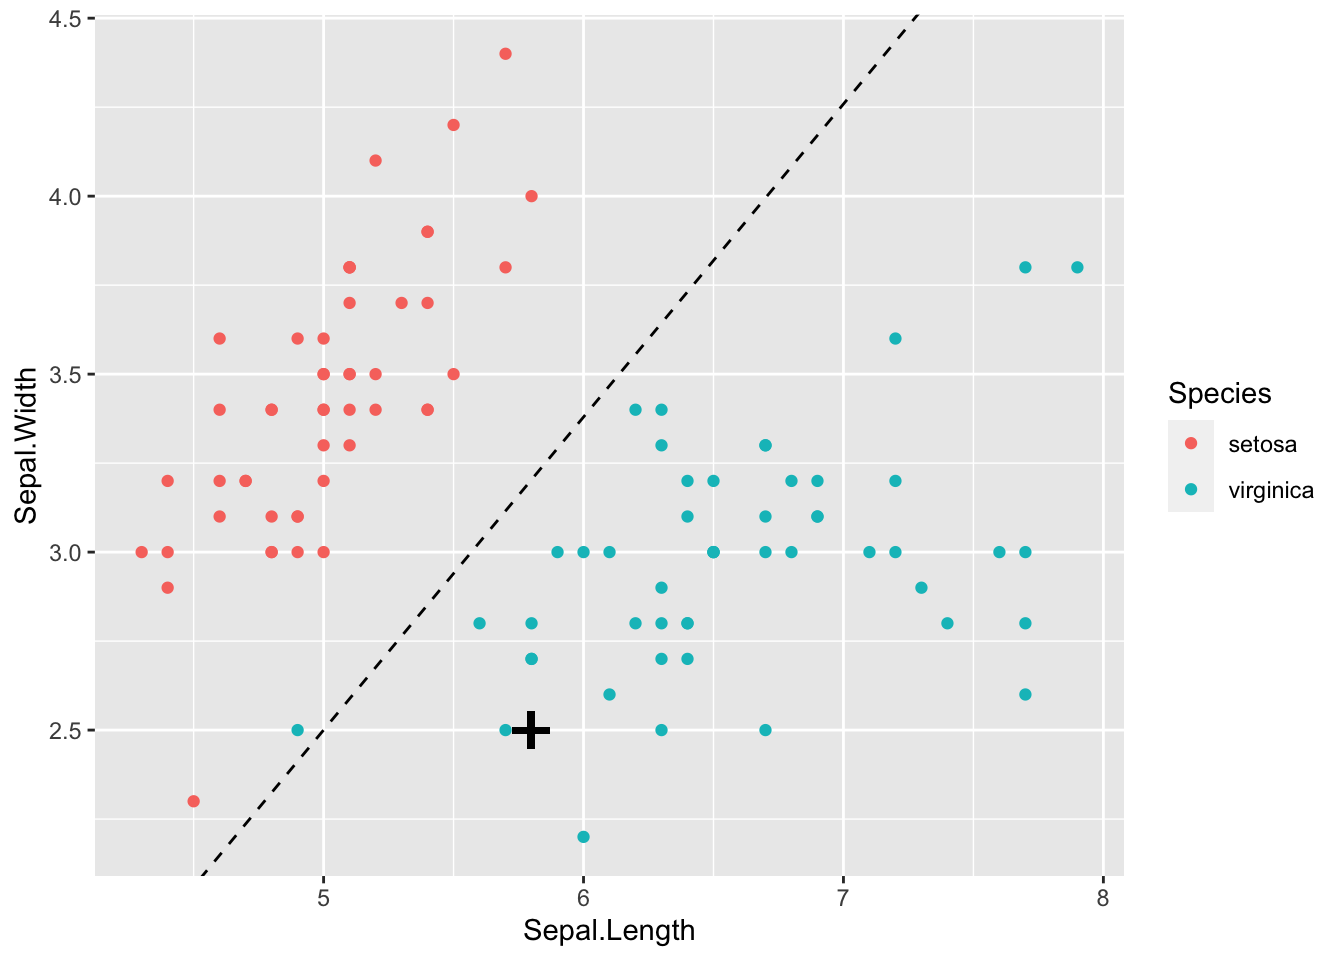
\includegraphics[width=1\linewidth]{03-matrix-decompositions_files/figure-latex/unnamed-chunk-12-1}

This is a \(512 \times 512\) colour image, meaning that there are three matrices \(\boldsymbol R, \boldsymbol B,\boldsymbol G\) of dimension \(512\times 512\)) giving the intensity of red, green, and blue for each pixel.
Naively storing this matrix requires 5.7Mb.

We can compute the SVD of the three colour intensity matrices, and the view the image that results from using reduced rank versions \(\boldsymbol B_k, \boldsymbol G_k, \boldsymbol R_k\) instead (as in Equation \eqref{eq:svdreduced}). The image below is formed using \(k=5, 30, 100\), and \(300\) basis vectors.

\begin{Shaded}
\begin{Highlighting}[]
\NormalTok{svd_image <-}\StringTok{ }\ControlFlowTok{function}\NormalTok{(im,k)\{}
\NormalTok{  s <-}\StringTok{ }\KeywordTok{svd}\NormalTok{(im)}
\NormalTok{  Sigma_k <-}\StringTok{ }\KeywordTok{diag}\NormalTok{(s}\OperatorTok{$}\NormalTok{d[}\DecValTok{1}\OperatorTok{:}\NormalTok{k])}
\NormalTok{  U_k <-}\StringTok{ }\NormalTok{s}\OperatorTok{$}\NormalTok{u[,}\DecValTok{1}\OperatorTok{:}\NormalTok{k]}
\NormalTok{  V_k <-}\StringTok{ }\NormalTok{s}\OperatorTok{$}\NormalTok{v[,}\DecValTok{1}\OperatorTok{:}\NormalTok{k]}
\NormalTok{  im_k <-}\StringTok{ }\NormalTok{U_k }\OperatorTok\StringTok{ }\NormalTok{Sigma_k }\OperatorTok\StringTok{ }\KeywordTok{t}\NormalTok{(V_k)}
   \CommentTok{## the reduced rank SVD produces some intensities <0 and >1. }
  \CommentTok{# Let's truncate these}
\NormalTok{  im_k[im_k}\OperatorTok{>}\DecValTok{1}\NormalTok{]=}\DecValTok{1}
\NormalTok{  im_k[im_k}\OperatorTok{<}\DecValTok{0}\NormalTok{]=}\DecValTok{0}
  \KeywordTok{return}\NormalTok{(im_k)}
\NormalTok{\}}

\KeywordTok{par}\NormalTok{(}\DataTypeTok{mfrow=}\KeywordTok{c}\NormalTok{(}\DecValTok{2}\NormalTok{,}\DecValTok{2}\NormalTok{), }\DataTypeTok{mar=}\KeywordTok{c}\NormalTok{(}\DecValTok{1}\NormalTok{,}\DecValTok{1}\NormalTok{,}\DecValTok{1}\NormalTok{,}\DecValTok{1}\NormalTok{))}

\NormalTok{pepprssvd<-}\StringTok{ }\NormalTok{peppers}
\ControlFlowTok{for}\NormalTok{(k }\ControlFlowTok{in} \KeywordTok{c}\NormalTok{(}\DecValTok{4}\NormalTok{,}\DecValTok{30}\NormalTok{,}\DecValTok{100}\NormalTok{,}\DecValTok{300}\NormalTok{))\{}
\NormalTok{  svds<-}\KeywordTok{list}\NormalTok{()}
  \ControlFlowTok{for}\NormalTok{(ii }\ControlFlowTok{in} \DecValTok{1}\OperatorTok{:}\DecValTok{3}\NormalTok{) \{}
\NormalTok{    pepprssvd[,,ii]<-}\KeywordTok{svd_image}\NormalTok{(peppers[,,ii],k)}
\NormalTok{  \}}
  \KeywordTok{plot}\NormalTok{(}\KeywordTok{as.raster}\NormalTok{(pepprssvd))}
\NormalTok{\}}
\end{Highlighting}
\end{Shaded}

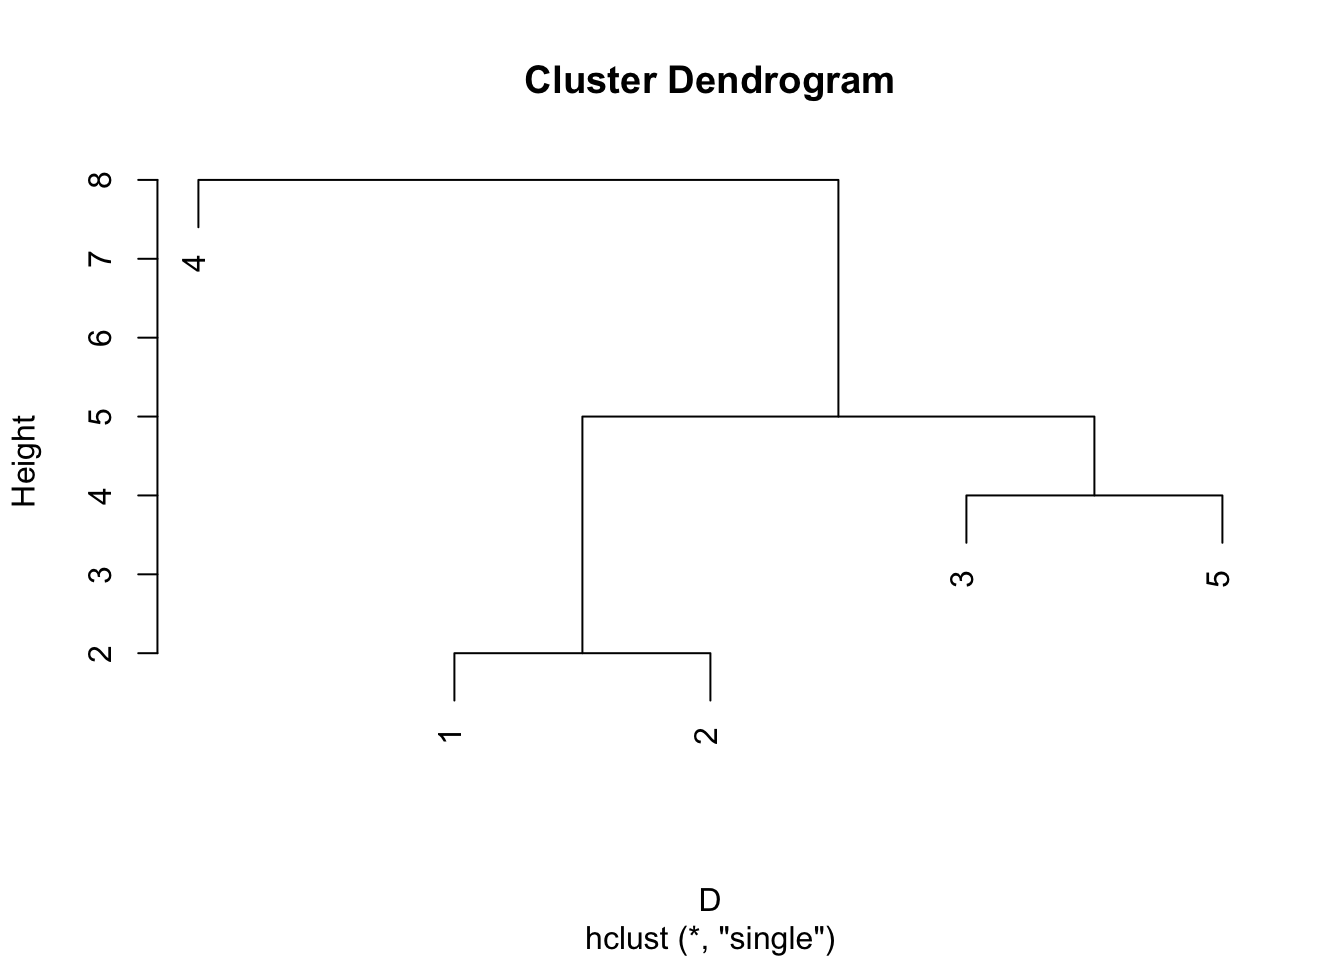
\includegraphics[width=1\linewidth]{03-matrix-decompositions_files/figure-latex/unnamed-chunk-13-1}

You can see that for \(k=30\) we have a reasonable approximation, but with some errors. With \(k=100\) it is hard to spot the difference with the original. The size of the four compressed images is 45Kb, 345Kb, 1.1Mb and 3.4Mb.

You can see further demonstrations of image compression with the SVD \href{http://timbaumann.info/svd-image-compression-demo/}{here}.

We will see much more of the SVD in later chapters.

\hypertarget{tasks-ch3}{%
\section{Computer tasks}\label{tasks-ch3}}

\begin{enumerate}
\def\labelenumi{\arabic{enumi}.}
\tightlist
\item
  Finding the eigenvalues and eigenvectors of a matrix is easy in R.
\end{enumerate}

\begin{Shaded}
\begin{Highlighting}[]
\NormalTok{A=}\KeywordTok{matrix}\NormalTok{(}\KeywordTok{c}\NormalTok{(}\DecValTok{3}\NormalTok{,}\DecValTok{1}\NormalTok{,}\DecValTok{1}\NormalTok{,}\DecValTok{6}\NormalTok{),}\DataTypeTok{nrow=}\DecValTok{2}\NormalTok{,}\DataTypeTok{byrow=}\OtherTok{TRUE}\NormalTok{)    }\CommentTok{# use a to define a matrix A}
\NormalTok{Eig=}\KeywordTok{eigen}\NormalTok{(A)                     }\CommentTok{# the eigenvalues and eigenvectors of A}
                                   \CommentTok{# are stored in the list Eig}
\NormalTok{lambda=Eig}\OperatorTok{$}\NormalTok{values                }\CommentTok{# extract the eigenvalues from Eig and}
                                   \CommentTok{# store in the vector e}
\NormalTok{lambda                           }\CommentTok{# you should see the eigenvalues in}
\end{Highlighting}
\end{Shaded}

\begin{verbatim}
## [1] 6.302776 2.697224
\end{verbatim}

\begin{Shaded}
\begin{Highlighting}[]
                                   \CommentTok{# descending order}
\NormalTok{Q=Eig}\OperatorTok{$}\NormalTok{vectors                    }\CommentTok{# extract the eigenvectors from Eig and}
                                   \CommentTok{# store then in the columns of Q}
\end{Highlighting}
\end{Shaded}

\begin{verbatim}
 The spectral decomposition of $\bA$ is 
\end{verbatim}

\[\boldsymbol A= \boldsymbol Q\boldsymbol \Lambda\boldsymbol Q^\top\]
Let's check this in R (noting as always that there may be some numerical errors)

\begin{Shaded}
\begin{Highlighting}[]
\NormalTok{Q}\OperatorTok\KeywordTok{diag}\NormalTok{(lambda)}\OperatorTok\KeywordTok{t}\NormalTok{(Q)          }\CommentTok{# reconstruct A,}
\end{Highlighting}
\end{Shaded}

\begin{verbatim}
##      [,1] [,2]
## [1,]    3    1
## [2,]    1    6
\end{verbatim}

\begin{Shaded}
\begin{Highlighting}[]
                                   \CommentTok{# where t(Q) gives the transpose of Q}
\end{Highlighting}
\end{Shaded}

\begin{verbatim}
 Since A is positive definite, we can calculate the symmetric, positive definite square root of A.
\end{verbatim}

\begin{Shaded}
\begin{Highlighting}[]
\NormalTok{Asqrt=Q}\OperatorTok\KeywordTok{diag}\NormalTok{(lambda}\OperatorTok{**}\FloatTok{0.5}\NormalTok{)}\OperatorTok\KeywordTok{t}\NormalTok{(Q) }\CommentTok{# lambda**0.5 contains the square roots}
\NormalTok{Asqrt}\OperatorTok\NormalTok{Asqrt                      }\CommentTok{# it is seen that A is recovered}
\end{Highlighting}
\end{Shaded}

\begin{verbatim}
##      [,1] [,2]
## [1,]    3    1
## [2,]    1    6
\end{verbatim}

\begin{verbatim}
 - Instead of using the full eigendecomposition for $\bA$, try truncating it and using just a single eigenvalue and eigenvector, i.e., compute
\end{verbatim}

\[\boldsymbol A' = \lambda_1 \boldsymbol q_1 \boldsymbol q_1^\top\]
- Compute the difference between \(\boldsymbol A\) and \(\boldsymbol A'\) using the 2-norm and the Frobenius norm.

\begin{enumerate}
\def\labelenumi{\arabic{enumi}.}
\setcounter{enumi}{1}
\tightlist
\item
  The singular value decomposition can be computed in R using the command \texttt{svd}. Let \(\boldsymbol X\) be the four numerical variables in the \texttt{iris} dataset with the column mean removed
\end{enumerate}

\begin{Shaded}
\begin{Highlighting}[]
\NormalTok{n=}\DecValTok{150}
\NormalTok{H=}\KeywordTok{diag}\NormalTok{(}\KeywordTok{rep}\NormalTok{(}\DecValTok{1}\NormalTok{,n))}\OperatorTok{-}\KeywordTok{rep}\NormalTok{(}\DecValTok{1}\NormalTok{,n)}\OperatorTok\KeywordTok{t}\NormalTok{(}\KeywordTok{rep}\NormalTok{(}\DecValTok{1}\NormalTok{,n))}\OperatorTok{/}\NormalTok{n   }\CommentTok{# calculate the centering matrix H}
\NormalTok{X=H}\OperatorTok\StringTok{ }\KeywordTok{as.matrix}\NormalTok{(iris[,}\DecValTok{1}\OperatorTok{:}\DecValTok{4}\NormalTok{])}
\CommentTok{# This can also be done using the command}
\CommentTok{# sweep(iris[,1:4], 2, colMeans(iris[,1:4]))  # do you understand why?}
\end{Highlighting}
\end{Shaded}

\begin{verbatim}
- Compute the SVD of $\bX$ in R and report its singular values.

- Does R report the full or  compact SVD?


- Check that $\bX \bv = \sigma \bu$.


- Compute the best rank-1, rank-2, and rank-3 approximations to $\bX$, and report the 2-norm and Frobenious norm for these approximations

- Compute the eigenvalues of $\bX^\top \bX$. How do these relate to the singular values? How does  $\bX^\top \bX$ relate to the sample covariance matrix of the iris data? How do the singular values relate to the eigenvalues of the covariance matrix?

- Let $\bS$ be the sample covariance matrix of the iris dataset. What vector maximizes $\bx \bS\bx$? 
\end{verbatim}

\begin{enumerate}
\def\labelenumi{\arabic{enumi}.}
\setcounter{enumi}{2}
\tightlist
\item
  Choose an few images from the \href{http://sipi.usc.edu/database/}{USC-SIPI Image Database} and repeat the image compression example from the notes. Which type of images compress well do you think?
\end{enumerate}

\hypertarget{exercises-ch3}{%
\section{Exercises}\label{exercises-ch3}}

\begin{enumerate}
\def\labelenumi{\arabic{enumi}.}
\tightlist
\item
  Compute, by hand (but check your answer in R), the singular value decomposition (full and compact) of the following matrices.

  \begin{itemize}
  \tightlist
  \item
    \(\left(\begin{array}{cc}2&0\\0&-1\end{array} \right)\)
  \item
    \(\left(\begin{array}{cc}1&0\\0&0\\0&0\end{array} \right)\)
  \end{itemize}
\item
  Let \[\boldsymbol X=\left(\begin{array}{cc}1&1\\0&1\\1&0\end{array}
  \right)\]\\
  The eigen-decomposition of \(\boldsymbol X^\top \boldsymbol X\) is
  \[\boldsymbol X^\top \boldsymbol X=\frac{1}{\sqrt{2}}\left(\begin{array}{cc}1&-1\\1&1\end{array}
  \right) \left(\begin{array}{cc}3&0\\0&1\end{array}
  \right)\frac{1}{\sqrt{2}}\left(\begin{array}{cc}1&-1\\1&1\end{array}
  \right)^\top \]
  Use this fact to compute the following:

  \begin{itemize}
  \tightlist
  \item
    What are the singular values of \(\boldsymbol X\)?
  \item
    What are the right singular vectors of \(\boldsymbol X\)?
  \item
    What are the left singular vectors of \(\boldsymbol X\)?
  \item
    Give the compact SVD of \(\boldsymbol X\). Check your answer, noting that the singular vectors are only specified up to multiplication by \(-1\)
  \item
    Can you compute the full SVD of \(\boldsymbol X\)?
  \item
    What is the eigen-decomposition of \(\boldsymbol X\boldsymbol X^\top\)?
  \item
    Find a generalised inverse of matrix \(\boldsymbol X\).
  \end{itemize}
\end{enumerate}

\begin{enumerate}
\def\labelenumi{\arabic{enumi}.}
\setcounter{enumi}{2}
\item
  The SVD can be used to solve linear systems of the form
  \[\boldsymbol A\boldsymbol x= \boldsymbol y\]
  where \(\boldsymbol A\) is a \(n\times p\) matrix, with compact SVD
  \(\boldsymbol A= \boldsymbol U\boldsymbol \Sigma\boldsymbol V^\top\).

  \begin{itemize}
  \item
    If \(\boldsymbol A\) is a square invertible matrix, show that \[\tilde{\boldsymbol x} = \boldsymbol V\boldsymbol \Sigma^{-1} \boldsymbol U^\top \boldsymbol y\] is the unique solution to \(\boldsymbol A\boldsymbol x= \boldsymbol y\), i.e., show that \(\boldsymbol A^{-1} = \boldsymbol V\boldsymbol \Sigma^{-1} \boldsymbol U^\top\).
  \item
    If \(\boldsymbol A\) is not a square matrix, then \(\boldsymbol A^+ = \boldsymbol V\boldsymbol \Sigma^{-1} \boldsymbol U^\top\) is a generalized inverse (not a true inverse) matrix, and
    \(\tilde{\boldsymbol x}=\boldsymbol A^+\boldsymbol y\) is still a useful quantity to consider as we shall now see. Let \(\boldsymbol A=\left(\begin{array}{cc}1&1\\0&1\\1&0\end{array} \right)\) and \(\boldsymbol y= \left(\begin{array}{c}2\\1\\1\end{array} \right)\). Then \(\boldsymbol A\boldsymbol x=\boldsymbol y\) is an over-determined system in that there are 3 equations in 2 unknowns. Compute \(\tilde{\boldsymbol x}=\boldsymbol A^+\boldsymbol y\). Is this a solution to the equation?
  \end{itemize}

  \textbf{Note} that you computed the svd for \(\boldsymbol A\) in the question 2.

  \begin{itemize}
  \tightlist
  \item
    Now suppose \(\boldsymbol y= \left(\begin{array}{c}1\\-1\\1\end{array} \right)\). There is no solution to \(\boldsymbol A\boldsymbol x=\boldsymbol y\) in this case as \(\boldsymbol y\) is not in the column space of \(\boldsymbol A\). Prove that \({\tilde{\boldsymbol x}} = \boldsymbol A^+\boldsymbol y\) solves the least squares problem
    \[\tilde{\boldsymbol x} = \arg\min_{\boldsymbol x}||\boldsymbol y- \boldsymbol A\boldsymbol x||_2.\]
  \end{itemize}

  \textbf{Hint}: You can either do this directly for this problem, or you can show that the least squares solution \((\boldsymbol A^\top \boldsymbol A)^{-1}\boldsymbol A^\top \boldsymbol y=\tilde{\boldsymbol x}\).
\item
  Consider the system
  \[\boldsymbol B\boldsymbol x= \boldsymbol y\mbox{ with }\boldsymbol B=\left(\begin{array}{ccc}1&0&1\\1&1&0\end{array}
  \right),\boldsymbol y= \left(\begin{array}{c}1\\1\end{array}
  \right).\]
  This is an underdetermined system, as there are 2 equations in 3 unknowns, and so there are an infinite number of solutions for \(\boldsymbol x\) in this case.

  \begin{itemize}
  \tightlist
  \item
    Find the full SVD for \(\boldsymbol B=\boldsymbol U\boldsymbol \Sigma\boldsymbol V^\top\) (noting that \(\boldsymbol B=\boldsymbol A^\top\) for \(\boldsymbol A\) from the previous question).
  \item
    Compute
    \(\tilde{\boldsymbol x}=\boldsymbol B^+\boldsymbol y\), check it is a solution to the equation, and explain why \[\tilde{\boldsymbol x}= \sum_{i=1}^r \boldsymbol v_i \frac{\boldsymbol u_i^\top \boldsymbol y}{\sigma_i}\] in general, where \(r\leq max(n,p)\) is the rank of \(\boldsymbol B\), and write out \(\tilde{\boldsymbol x}\) explicitly in this form for the given \(\boldsymbol B\).
  \item
    Consider \(\boldsymbol x\) of the form
    \[\boldsymbol x= \tilde{\boldsymbol x} + \sum_{i=r+1}^n \alpha_i \boldsymbol v_i\]
    and explain why any \(\boldsymbol x\) of this form is also a solution to \(\boldsymbol B\boldsymbol x=\boldsymbol y\). Thus write out all possible solutions of the equation.
  \item
    Prove that \(\tilde{\boldsymbol x}\) is the solution with minimum norm, i.e., \(||\tilde{\boldsymbol x}||_2 \leq ||\boldsymbol x||_2\). \textbf{Hint} \(\boldsymbol v_1, \ldots, \boldsymbol v_p\) form a complete orthonormal basis for \(\mathbb{R}^p\).
  \end{itemize}
\item
  Prove proposition \ref{prp:eigproj}.
\end{enumerate}

\hypertarget{part-ii-dimension-reduction-methods}{%
\chapter*{PART II: Dimension reduction methods}\label{part-ii-dimension-reduction-methods}}
\addcontentsline{toc}{chapter}{PART II: Dimension reduction methods}

In many applications, a large number of variables are recorded for each experimental unit under study. For example, if we think of individual people as the \emph{experimental units}, then in a health check-up we might collect data on age, blood pressure, cholesterol level, blood test results, lung function, weight, height, BMI, etc. If you use websites such as Amazon, Facebook, and Google, they store thousands (possibly millions) of pieces of information about you (\href{https://www.theguardian.com/commentisfree/2018/mar/28/all-the-data-facebook-google-has-on-you-privacy}{this article} shows you how to download the information Google stores about you, including all the locations you've visited, every search, youtube video, or app you've used and more). They process this data to create an individual profile for each user, which they can then use to create targetted adverts.

When analysing data of moderate or high dimension, it is often desirable to seeks ways to restructure the data and reduce its dimension whilst \textbf{retaining the most important information} within the data or \textbf{preserving some feature of interest} in the data. There a variety of reasons we might want to do this.

\begin{itemize}
\tightlist
\item
  In reduced dimensions, it is often much easier to understand and appreciate the most important features of a dataset.
\item
  If there is a lot of reduncancy in the data, we might want to reduce the dimension to lower the memory requirements in storing it (e.g.~with sound and image compression).
\item
  In high dimensions, it can be difficult to analyse data (e.g.~with statistical methods), and so reducing the dimension can be a way to make a dataset amenable to analysis.
\end{itemize}

In this part of the module we investigate three different methods for dimension reduction: Principal Component Analysis (PCA) in Chapter \ref{pca}; Canonical Correlation Analysis (CCA) in Chapter \ref{cca}; and Multidimensional Scaling (MDS) in Chapter \ref{mds}. Matrix algebra (Chapters \ref{linalg-prelim} and \ref{linalg-decomp}) plays a key role in all three of these techniques.

\hypertarget{a-warning}{%
\subsection*{A warning}\label{a-warning}}
\addcontentsline{toc}{subsection}{A warning}

Beware that high-dimensional data can behave qualitatively differently to low-dimensional data. As an example, lets consider 1000 points uniformly distributed in \([0,1]^d\), and think about how close together or spread out the points are. A simple way to do this is to consider the ratio of the maximum and minimum distance between any two points in our sample.

\begin{Shaded}
\begin{Highlighting}[]
\NormalTok{N<-}\DecValTok{1000}
\NormalTok{averatio <-}\KeywordTok{c}\NormalTok{()}
\NormalTok{ii<-}\DecValTok{1}
\ControlFlowTok{for}\NormalTok{(d }\ControlFlowTok{in} \KeywordTok{c}\NormalTok{(}\DecValTok{2}\NormalTok{,}\DecValTok{5}\NormalTok{,}\DecValTok{10}\NormalTok{,}\DecValTok{20}\NormalTok{,}\DecValTok{30}\NormalTok{,}\DecValTok{40}\NormalTok{,}\DecValTok{50}\NormalTok{,}\DecValTok{60}\NormalTok{,}\DecValTok{80}\NormalTok{,}\DecValTok{100}\NormalTok{, }\DecValTok{200}\NormalTok{, }\DecValTok{350}\NormalTok{, }\DecValTok{500}\NormalTok{, }\DecValTok{750}\NormalTok{, }\DecValTok{1000}\NormalTok{))\{}
\NormalTok{  averatio[ii] <-}\StringTok{ }\KeywordTok{mean}\NormalTok{(}\KeywordTok{replicate}\NormalTok{(}\DecValTok{10}\NormalTok{, \{}
\NormalTok{  X<-}\KeywordTok{matrix}\NormalTok{(}\KeywordTok{runif}\NormalTok{(N}\OperatorTok{*}\NormalTok{d), }\DataTypeTok{nc=}\NormalTok{d)}
\NormalTok{  d <-}\StringTok{ }\KeywordTok{as.matrix}\NormalTok{(}\KeywordTok{dist}\NormalTok{(X)) }
  \CommentTok{# this gives a N x N matrix of the Euclidean distances between the data points.}
\NormalTok{  maxdist <-}\StringTok{ }\KeywordTok{max}\NormalTok{(d) }
\NormalTok{  mindist <-}\StringTok{ }\KeywordTok{min}\NormalTok{(d}\OperatorTok{+}\KeywordTok{diag}\NormalTok{(}\DecValTok{10}\OperatorTok{^}\DecValTok{5}\NormalTok{, }\DataTypeTok{nrow=}\NormalTok{N)) }
  \CommentTok{# The diagonal elements of the distance matrix are zero,}
  \CommentTok{# so I've added a big number to the diagonal }
  \CommentTok{# so that we get the minimum distance between different points}
\NormalTok{  maxdist}\OperatorTok{/}\NormalTok{mindist\}))}
\NormalTok{  ii <-}\StringTok{ }\NormalTok{ii}\OperatorTok{+}\DecValTok{1}
\NormalTok{\}}
\KeywordTok{plot}\NormalTok{(}\KeywordTok{c}\NormalTok{(}\DecValTok{2}\NormalTok{,}\DecValTok{5}\NormalTok{,}\DecValTok{10}\NormalTok{,}\DecValTok{20}\NormalTok{,}\DecValTok{30}\NormalTok{,}\DecValTok{40}\NormalTok{,}\DecValTok{50}\NormalTok{,}\DecValTok{60}\NormalTok{,}\DecValTok{80}\NormalTok{,}\DecValTok{100}\NormalTok{, }\DecValTok{200}\NormalTok{, }\DecValTok{350}\NormalTok{, }\DecValTok{500}\NormalTok{, }\DecValTok{750}\NormalTok{, }\DecValTok{1000}\NormalTok{), }
\NormalTok{     averatio, }\DataTypeTok{ylab=}\StringTok{'Max. dist. / min. dist.'}\NormalTok{, }\DataTypeTok{xlab=}\StringTok{'Dimension d'}\NormalTok{, }\DataTypeTok{log=}\StringTok{'xy'}\NormalTok{)}
\end{Highlighting}
\end{Shaded}

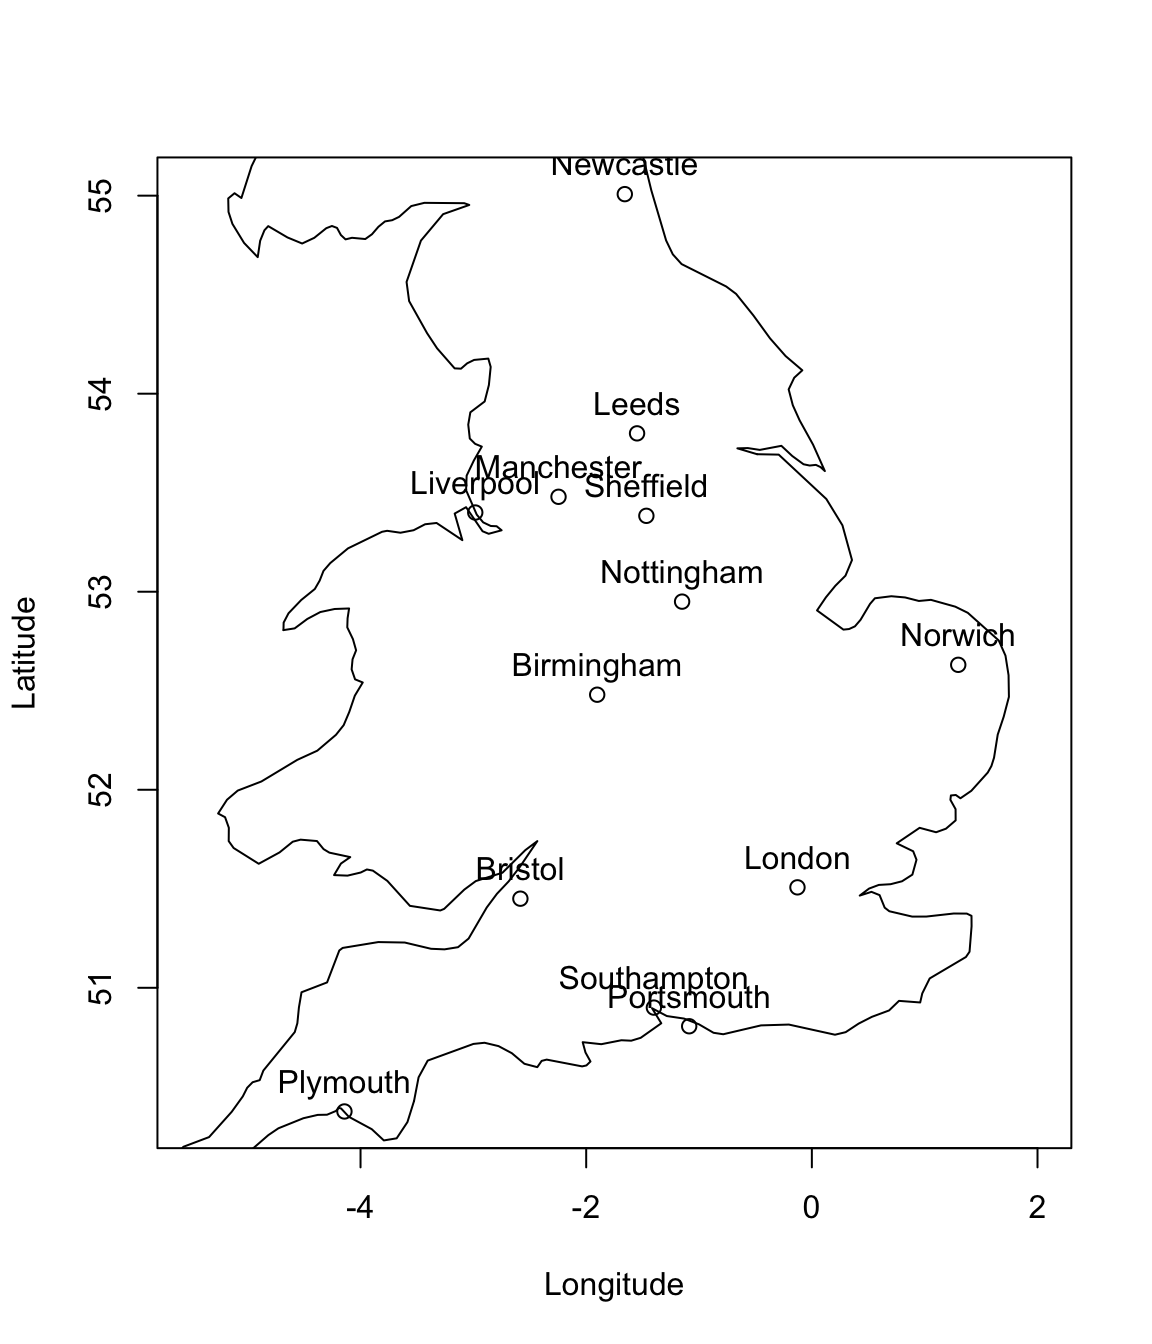
\includegraphics{04-pca_files/figure-latex/unnamed-chunk-1-1.pdf}

So we can see that as the dimension increases, the ratio of the maximum and minimum distance between any two random points in our sample tends to 1. In other words, all points are the same distance apart!

\hypertarget{pca}{%
\chapter{Principal component analysis (PCA)}\label{pca}}

With multivariate data, it is common to want to reduce the dimension of the data \emph{in a sensible way}. For example

\begin{itemize}
\item
  exam marks across different modules are
  averaged to produce a single overall mark for each
  student
\item
  a football league table converts the
  numbers of wins, draws and losses to a single measure of
  points.
\end{itemize}

Mathematically, these summaries
are both linear combinations of the
original variables of the form
\[y = \boldsymbol u^\top \boldsymbol x.\]\\
for some choice of \(\boldsymbol u\).

For the exam marks example, suppose each student sits \(p=4\) modules
with marks, \(x_1,x_2,x_3,x_4\). Then, writing \(\boldsymbol x=(x_1, x_2 , x_3, x_4)^\top\) and choosing \(\boldsymbol u= \left(\frac{1}{4}, \frac{1}{4}, \frac{1}{4}, \frac{1}{4} \right)^\top\)
gives an overall average,
\[ y =\boldsymbol u^\top \boldsymbol x= \begin{pmatrix} \frac{1}{4} & \frac{1}{4} & \frac{1}{4} & \frac{1}{4} \end{pmatrix} \begin{pmatrix} x_1 \\ x_2 \\ x_3 \\ x_4 \end{pmatrix} = \frac{x_1}{4} + \frac{x_2}{4} + \frac{x_3}{4} + \frac{x_4}{4}.\]

For the football league table, if \(w\) is the number of wins, \(d\) is the number of draws and \(l\) is the number of losses then, writing
\({\mathbf r}=(w,d,l)^\top\), we choose \(\boldsymbol u= \left(3,1,0 \right)^\top\) to get the points score
\[ y = \boldsymbol u^\top {\mathbf r}=\begin{pmatrix} 3 & 1 & 0 \end{pmatrix} \begin{pmatrix} w \\ d \\ l \end{pmatrix} = 3w + 1d + 0l=3w+d.\]

\hypertarget{geometric-interpretation}{%
\subsubsection*{Geometric interpretation}\label{geometric-interpretation}}
\addcontentsline{toc}{subsubsection}{Geometric interpretation}

In the two examples above, we used the vector \(\boldsymbol u\) to convert our original variables, \(\boldsymbol x\),
to a new variable, \(y\), by projecting \(\boldsymbol x\) onto \(\boldsymbol u\).
We can think of this as a projection onto the subspace defined by \(\boldsymbol u\)

\[U = \operatorname{span}\{\boldsymbol u\} = \{\lambda \boldsymbol u: \lambda \in \mathbb{R}\}\subset \mathbb{R}^p,\]

For the exam data, each data point \(\boldsymbol x= \begin{pmatrix} x_1 \\ x_2 \\ x_3 \\ x_4 \end{pmatrix}\)
is a vector in \(\mathbb{R}^4\), and we've expressed \(\boldsymbol x\) in terms of its coordinates with respsect to the standard basis, \(\boldsymbol e_1^\top = (1\; 0\; 0 \; 0)\) etc:
\[\boldsymbol x=x_1 \boldsymbol e_1 + x_2 \boldsymbol e_2 +x_3 \boldsymbol e_3 +x_4 \boldsymbol e_4.\]
The vector subspace \(U\) is a line in \(\mathbb{R}^4\) along the direction \(\boldsymbol u= \begin{pmatrix} \frac{1}{4} & \frac{1}{4} & \frac{1}{4} & \frac{1}{4} \end{pmatrix}^\top\).

How do we project onto subspace \(U\)?

\begin{itemize}
\tightlist
\item
  If \(||\boldsymbol u||_2=1\) then the orthogonal projection of \(\boldsymbol x\) onto \(U\) is\\
  \[\boldsymbol u\boldsymbol u^\top\boldsymbol x.\]
  Or in other words, the projection of \(\boldsymbol x\) onto subspace \(U\) has coordinate \(\boldsymbol u^\top \boldsymbol x\) with respect to basis \(\{\boldsymbol u\}\).
\end{itemize}

If you prefer to think in terms of projection matrices (see Chapter \ref{orthogproj}), then the matrix for projecting onto \(U\) is
\[\boldsymbol P_U = \boldsymbol u(\boldsymbol u^\top \boldsymbol u)^{-1}\boldsymbol u^\top\]
which simplifies to
\[\boldsymbol P_U = \boldsymbol u\boldsymbol u^\top\]
when \(||\boldsymbol u||=\sqrt{\boldsymbol u^\top\boldsymbol u}=1\) so that we again see the projection of \(\boldsymbol x\) onto \(U\) is \(y=\boldsymbol P_u \boldsymbol x= \boldsymbol u\boldsymbol u^\top\boldsymbol x\).

\textbf{How should we choose \(\boldsymbol u\)?}

The answer to that question depends upon the goal of the analysis. For the exam and football league examples, the choice of \(\boldsymbol u\) is an arbitrary decision taken in order to reduce a multidimensional dataset to a single variable (average mark, or points).

A single \(\boldsymbol u\) gives a \textbf{snapshot} or summary of the data. If \(\boldsymbol u\) is chosen well that snapshot may tell us much of what we want to know about the data, e.g.,

\begin{itemize}
\tightlist
\item
  Liverpool won the league,
\item
  student \(X\)'s exam performance was first class etc.
\end{itemize}

In many cases we will want to use multiple snapshots: instead of using a single \(\boldsymbol u\), we will use a collection \(\boldsymbol u_1, \boldsymbol u_2, \ldots, \boldsymbol u_r\) and consider the derived variables

\[\boldsymbol y= \begin{pmatrix} y_1\\y_2 \\ \vdots \\ y_r\end{pmatrix} = \begin{pmatrix}
\boldsymbol u_1^\top \boldsymbol x\\  \boldsymbol u_2^\top \boldsymbol x\\\vdots\\  \boldsymbol u_r^\top \boldsymbol x\end{pmatrix}\]

In matrix notation, if we set
\[\boldsymbol U= \begin{pmatrix} 
|&&|\\
\boldsymbol u_1 & \ldots & \boldsymbol u_r\\
|&&|\end{pmatrix}\]
then the new derived variable is
\[\boldsymbol y= \boldsymbol U^\top \boldsymbol x.\]

If \(\dim(\boldsymbol y)=r<p=\dim(\boldsymbol x)\) then we have reduced the dimension of the data. If \(\boldsymbol y\) tells us all we need to know about the data, then we can work (plot, analyse, model) with \(\boldsymbol y\) instead of \(\boldsymbol x\). If \(r\ll p\) this can make working with the data significantly easier, as we can more easily visulise and understand low dimensional problems.

We will study a variety of methods for choosing \(\boldsymbol U\). The methods can all be expressed as constrained optimization problems:

\begin{align}
\mbox{minimize} f_{\boldsymbol X}(\boldsymbol U) \label{eq:dimredopt} \\
\mbox{ subject to } \boldsymbol U\in \mathcal{U} 
\end{align}

The objective \(f_{\boldsymbol X}(\boldsymbol U)\) varies between methods: principal component analysis (PCA) maximizes variance or minimizes reconstruction error; canonical correlation analysis (CCA) maximizes correlation; multidimensional scaling (MDS) maximizes spread etc.

The contstraint on the search space \(\mathcal{U}\), is usually that \(\boldsymbol U\) must be (partially) orthogonal, but in other methods other constraints are used

\hypertarget{pca-an-informal-introduction}{%
\section{PCA: an informal introduction}\label{pca-an-informal-introduction}}

There are two different ways of motivating
principal component analysis (PCA), which may in part explain why PCA is so widely used.

The first motivation, and the topic of this section, is to introduce PCA as method for maximizing the variance of the transformed variables \(\boldsymbol y\). We start by choosing \(\boldsymbol u_1\) so that \(y_1=\boldsymbol u_1^\top \boldsymbol x\) has maximum variance. We then choose \(\boldsymbol u_2\) so that \(y_2=\boldsymbol u_2^\top \boldsymbol x\) has maximum variance subject to being uncorrelated with \(y_1\), and so on.

The idea is to produce a set of variables \(y_1, y_2, \ldots, y_r\) that are uncorrelated, but which are most informative about the data. The thinking is that if a variable has large variance it must be informative/important.

The name \textbf{principal component analysis} comes from thinking of this as splitting the data \(\boldsymbol X\) into its most important parts. It therefore won't surprise you to find that this involves the matrix decompositions we studied in Chapter \ref{linalg-decomp}.

\href{https://twitter.com/allison_horst/status/1288904459490213888?lang=en}{Allison Horst (@allison\_horst)} gave a great illustration of how to think about PCA on Twitter. Imagine you are a whale shark with a wide mouth


\includegraphics{figs/WideMouthShark1.png}

and that you're swimming towards a delicious swarm of krill.


\includegraphics{figs/WideMouthShark2.png}

What way should you tilt your shark head in order to eat as many krill as possible? The answer is given by the first principal component of the data!

\hypertarget{notation-recap}{%
\subsection{Notation recap}\label{notation-recap}}

As before, let \(\boldsymbol x_1,\ldots,\boldsymbol x_n\) be \(p \times 1\) vectors of measurements on \(n\) experimental units and write
\[\boldsymbol X=\left( \begin{array}{ccc}
- &\boldsymbol x_1^\top&-\\
- &\boldsymbol x_2^\top&-\\
- &..&-\\
- &\boldsymbol x_n^\top&-
\end{array}\right)
\]

\textbf{IMPORTANT NOTE:}
In this section we will assume that \(\boldsymbol X\) has been column centered so that the mean of each column is \(0\) (i.e., the sample mean of \(\boldsymbol x_1,\ldots,\boldsymbol x_n\) is the zero vector \(\boldsymbol 0\in \mathbb{R}^p\)). If \(\boldsymbol X\) has not been column centered, replace \(\boldsymbol X\) by
\[\boldsymbol H\boldsymbol X\] where \(\boldsymbol H\) is the centering matrix (see \ref{centering-matrix}), or equivalently, replace \(\boldsymbol x_i\) by \(\boldsymbol x_i - \bar{\boldsymbol x}\). It is possible to write out the details of PCA replacing \(\boldsymbol X\) by \(\boldsymbol H\boldsymbol X\) throughout, but this gets messy and obscures the important detail. Most software implementations (and in particular \texttt{prcomp} in R), automatically centre your data for you, and so in practice you don't need to worry about doing this when using a software package.

The sample covariance matrix for \(\boldsymbol X\) (assuming it has been column centered) is
\[\boldsymbol S= \frac{1}{n}\boldsymbol X^\top \boldsymbol X= \frac{1}{n}\sum \boldsymbol x_i\boldsymbol x_i^\top\]

Given some vector \(\boldsymbol u\), the transformed variables
\[y_i = \boldsymbol u^\top \boldsymbol x_i\]
have

\begin{itemize}
\item
  \textbf{mean \(0\)}:
  \[\bar{y}= \frac{1}{n}\sum_{i=1}^n y_i = \frac{1}{n}\sum_{i=1}^n \boldsymbol u^\top \boldsymbol x_i =\frac{1}{n} \boldsymbol u^\top \sum_{i=1}^n  \boldsymbol x_i = 0\]
  as the mean of the \(\boldsymbol x_i\) is \(\boldsymbol 0\).
\item
  \textbf{sample covariance matrix} \[\boldsymbol u^\top \boldsymbol S\boldsymbol u\]
  as
  \[\frac{1}{n} \sum_{i=1}^n y_i^2 = \frac{1}{n} \sum_{i=1}^n \boldsymbol u^\top \boldsymbol x_i \boldsymbol x_i^\top\boldsymbol u= \frac{1}{n}\boldsymbol u^\top \sum_{i=1}^n  \boldsymbol x_i \boldsymbol x_i^\top \boldsymbol u= \boldsymbol u^\top \boldsymbol S\boldsymbol u
  \]
\end{itemize}

\hypertarget{first-principal-component}{%
\subsection{First principal component}\label{first-principal-component}}

We would like to find the \(\boldsymbol u\) which maximises the sample variance, \(\boldsymbol u^\top \boldsymbol S\boldsymbol u\) over unit vectors \(\boldsymbol u\), i.e., vectors with \(||\boldsymbol u||=1\). Why do we focus on unit vectors? If we don't, we could make the variance as large as we like, e.g., if we replace \(\boldsymbol u\) by \(10\boldsymbol u\) it would increase the variance by a factor of 100. Thus, we constrain the problem and only consider unit vectors for \(\boldsymbol u\).

We know from Proposition \ref{prp:two8} in Section \ref{svdopt} that \(\boldsymbol v_1\), the first eigenvector of \(\boldsymbol S\) (also the first right singular vector of \(\boldsymbol X\)), maximizes \(\boldsymbol u^\top \boldsymbol S\boldsymbol u\) with
\[  \max_{\boldsymbol u: ||\boldsymbol u||=1} \boldsymbol u^\top \boldsymbol S\boldsymbol u= \boldsymbol v_1 \boldsymbol S\boldsymbol v_1 =\lambda_1\]
where \(\lambda_1\) is the largest eigenvalue of \(\boldsymbol S\).

So the first principal component of \(\boldsymbol X\) is \(\boldsymbol v_1\), and the first transformed variable (sometimes called a principal component score) is \(y_1 = \boldsymbol v_1 ^\top \boldsymbol x\).
Applying this to each data point we get \(n\) instances of this new variable
\[y_{i1} = \boldsymbol v_1 ^\top \boldsymbol x_i.\]

\textbf{A note on singular values}: We know \(\boldsymbol S= \frac{1}{n}\boldsymbol X^\top\boldsymbol X\) and so the eigenvalues of \(\boldsymbol S\) are the same as the squared singular values of \(\frac{1}{\sqrt{n}} \boldsymbol X\):

\[\sqrt{\lambda_1} = \sigma_1\left(\frac{1}{\sqrt{n}} \boldsymbol X\right)\]

If we scale \(\boldsymbol X\) by a factor \(c\), then the singular values are scaled by the same amount, i.e.,
\[\sigma_i(c\boldsymbol X)=c\sigma_i(\boldsymbol X)\]
and in particular
\[ \sigma_i\left(\frac{1}{\sqrt{n}} \boldsymbol X\right) = \frac{1}{\sqrt{n}} \sigma_i(\boldsymbol X)\]
We will need to remember this scaling if we use the SVD of \(\boldsymbol X\) to do PCA. Note that scaling \(\boldsymbol X\) does not change the singular vectors/principal components.

\hypertarget{second-principal-component}{%
\subsection{Second principal component}\label{second-principal-component}}

\(y_1\) is the transformed variable that has maximum variance. What should we choose to be our next transformed variable, i.e., what \(\boldsymbol u_2\) should we choose for \(y_2 = \boldsymbol u_2^\top \boldsymbol x\)? It makes sense to choose \(y_2\) to be uncorrelated with \(y_1\), as otherwise it contains some of the same information given by \(y_1\). The sample covariance between \(y_1\) and \(\boldsymbol u_2^\top \boldsymbol x\) is
\begin{align*}
s_{y_2y_1} &=\frac{1}{n}\sum_{i=1}^n \boldsymbol u_2^\top \boldsymbol x_i \boldsymbol x_i^\top \boldsymbol v_1\\ 
&= \boldsymbol u_2^\top \boldsymbol S\boldsymbol v_1\\
& = \lambda_1 \boldsymbol u_2^\top \boldsymbol v_1 \mbox{ as } \boldsymbol v_1 \mbox{ is an eigenvector of } S
\end{align*}
So to make \(y_2\) uncorrelated with \(y_1\) we have to choose \(\boldsymbol u_2\) to be orthogonal to \(\boldsymbol v_1\), i.e., \(\boldsymbol u_2^\top \boldsymbol v_1=0\). So we choose \(\boldsymbol u_2\) to be the solution to the optimization problem

\[\max_{\boldsymbol u} \boldsymbol u^\top \boldsymbol S\boldsymbol u\mbox{ subject to } \boldsymbol u^\top \boldsymbol v_1=0.\]
The solution to this problem is to take \(\boldsymbol u_2 = \boldsymbol v_2\), i.e., the second eigenvector of \(\boldsymbol S\) (or second right singular vector of \(\boldsymbol X\)), and then \[\boldsymbol v_2^\top \boldsymbol S\boldsymbol v_2=\lambda_2.\]
We'll prove this result in the next section.

\hypertarget{later-principal-components}{%
\subsubsection*{Later principal components}\label{later-principal-components}}
\addcontentsline{toc}{subsubsection}{Later principal components}

Our first transformed variable is
\[y_{i1}= \boldsymbol v_1^\top \boldsymbol x_i\]
and our second transformed variable is
\[y_{i2}= \boldsymbol v_2^\top \boldsymbol x_i.\]
At this point, you can probably guess that the \(j^{th}\) transformed variable is going to be
\[y_{ij}= \boldsymbol v_j^\top \boldsymbol x_i.\]
where \(\boldsymbol v_j\) is the \(j^{th}\) eigenvector of \(\boldsymbol S\).

\begin{itemize}
\tightlist
\item
  The transformed variables \(y_{i}\) are the \textbf{principal component scores}. \(y_1\) is the first score etc.
\item
  The eigenvectors/right singular vectors are sometimes refered to as the \textbf{loadings} or simply as the \textbf{principal components}.
\end{itemize}

\hypertarget{geometric-interpretation-1}{%
\subsection{Geometric interpretation}\label{geometric-interpretation-1}}

We think of PCA as projecting the data points \(\boldsymbol x\) onto a subspace \(V\). The basis vectors for this subspace are the eigenvectors of \(\boldsymbol S\), which are the same as the right singular vectors of \(\boldsymbol X\) (the loadings):
\[V=\operatorname{span}\{\boldsymbol v_1, \ldots, \boldsymbol v_r\}.\]
The orthogonal projection matrix (see Section \ref{orthogproj}) for projecting onto \(V\) is
\[\boldsymbol P_V = \boldsymbol V\boldsymbol V^\top\]
as \(\boldsymbol V^\top \boldsymbol V=\mathbf I\).\\
The coordinates of the data points projected onto \(V\) (with respect to the basis for \(V\)) are the \textbf{principal component scores}:

\[\boldsymbol y_i= \left(\begin{array}{c}y_{i1}\\\vdots\\y_{ir}\end{array}\right)= \boldsymbol V^\top \boldsymbol x_i\]
where \[\boldsymbol V= \left(\begin{array}{ccc} | &&|\\\boldsymbol v_1&\ldots& \boldsymbol v_r\\  | &&|\end{array}\right)\]
is the matrix of right singular vectors from the SVD of \(\boldsymbol X\).
The transformed variables are

\[\boldsymbol Y= \left( \begin{array}{ccc}
- &\boldsymbol y_1^\top&-\\
- &..&-\\
- &\boldsymbol y_n^\top&-
\end{array}\right ) = \boldsymbol X\boldsymbol V.
\]
Substituting the SVD for \(\boldsymbol X= \boldsymbol U\boldsymbol \Sigma\boldsymbol V^\top\) we can see the transformed variable matrix/principal component scores are
\[\boldsymbol Y= \boldsymbol U\boldsymbol \Sigma.\]

\(\boldsymbol Y\) is a \(n \times r\) matrix, and so if \(r<p\) we have reduced the dimension of \(\boldsymbol X\), keeping the most important parts of the data

\hypertarget{example}{%
\subsection{Example}\label{example}}

We consider the marks of \(n=10\) students who studied G11PRB and G11STA.

\begin{table}[H]
\centering
\begin{tabular}{rrr}
\toprule
student & PRB & STA\\
\midrule
1 & 81 & 75\\
2 & 79 & 73\\
3 & 66 & 79\\
4 & 53 & 55\\
5 & 43 & 53\\
\addlinespace
6 & 59 & 49\\
7 & 62 & 72\\
8 & 79 & 92\\
9 & 49 & 58\\
10 & 55 & 56\\
\bottomrule
\end{tabular}
\end{table}

These data haven't been column centered, so let's do that in R. You can do it using the centering matrix as previously, but here is a different approach:

\begin{Shaded}
\begin{Highlighting}[]
\NormalTok{secondyr <-}\StringTok{ }\KeywordTok{data.frame}\NormalTok{(}
  \DataTypeTok{student =} \DecValTok{1}\OperatorTok{:}\DecValTok{10}\NormalTok{,}
\DataTypeTok{PRB=}\KeywordTok{c}\NormalTok{(}\DecValTok{81}\NormalTok{ , }\DecValTok{79}\NormalTok{ , }\DecValTok{66}\NormalTok{ , }\DecValTok{53}\NormalTok{ , }\DecValTok{43}\NormalTok{ , }\DecValTok{59}\NormalTok{ , }\DecValTok{62}\NormalTok{ , }\DecValTok{79}\NormalTok{ , }\DecValTok{49}\NormalTok{ , }\DecValTok{55}\NormalTok{),}
\DataTypeTok{STA =}\KeywordTok{c}\NormalTok{(}\DecValTok{75}\NormalTok{ , }\DecValTok{73}\NormalTok{ , }\DecValTok{79}\NormalTok{ , }\DecValTok{55}\NormalTok{ , }\DecValTok{53}\NormalTok{ , }\DecValTok{49}\NormalTok{ , }\DecValTok{72}\NormalTok{ , }\DecValTok{92}\NormalTok{ , }\DecValTok{58}\NormalTok{ , }\DecValTok{56}\NormalTok{)}
\NormalTok{        )}
\NormalTok{xbar <-}\StringTok{ }\KeywordTok{colMeans}\NormalTok{(secondyr[,}\DecValTok{2}\OperatorTok{:}\DecValTok{3}\NormalTok{]) }\CommentTok{#only columns 2 and 3 are data}
\NormalTok{X <-}\StringTok{ }\KeywordTok{as.matrix}\NormalTok{(}\KeywordTok{sweep}\NormalTok{(secondyr[,}\DecValTok{2}\OperatorTok{:}\DecValTok{3}\NormalTok{], }\DecValTok{2}\NormalTok{, xbar) )}
\end{Highlighting}
\end{Shaded}

\begin{table}[H]
\centering
\begin{tabular}{rr}
\toprule
PRB & STA\\
\midrule
18.4 & 8.8\\
16.4 & 6.8\\
3.4 & 12.8\\
-9.6 & -11.2\\
-19.6 & -13.2\\
\addlinespace
-3.6 & -17.2\\
-0.6 & 5.8\\
16.4 & 25.8\\
-13.6 & -8.2\\
-7.6 & -10.2\\
\bottomrule
\end{tabular}
\end{table}

The sample covariance matrix can be computed in two ways:

\begin{Shaded}
\begin{Highlighting}[]
\DecValTok{1}\OperatorTok{/}\DecValTok{10}\OperatorTok{*}\StringTok{ }\KeywordTok{t}\NormalTok{(X)}\OperatorTok\NormalTok{X}
\end{Highlighting}
\end{Shaded}

\begin{verbatim}
##        PRB    STA
## PRB 162.04 135.38
## STA 135.38 175.36
\end{verbatim}

\begin{Shaded}
\begin{Highlighting}[]
\KeywordTok{cov}\NormalTok{(X)}\OperatorTok{*}\DecValTok{9}\OperatorTok{/}\DecValTok{10} 
\end{Highlighting}
\end{Shaded}

\begin{verbatim}
##        PRB    STA
## PRB 162.04 135.38
## STA 135.38 175.36
\end{verbatim}

\begin{Shaded}
\begin{Highlighting}[]
\CommentTok{# Remember R uses the unbiased factor 1/(n-1), so the 9/10=(n-1)/n changes this to 1/n }
\CommentTok{# to match the notes}
\end{Highlighting}
\end{Shaded}

We can find the singular value decomposition of \(\boldsymbol X\) using R

\begin{Shaded}
\begin{Highlighting}[]
\NormalTok{(}\DataTypeTok{X_svd =} \KeywordTok{svd}\NormalTok{(X))}
\end{Highlighting}
\end{Shaded}

\begin{verbatim}
## $d
## [1] 55.15829 18.20887
## 
## $u
##              [,1]        [,2]
##  [1,] -0.34556317 -0.39864295
##  [2,] -0.29430029 -0.39482564
##  [3,] -0.21057607  0.34946080
##  [4,]  0.26707104 -0.04226416
##  [5,]  0.41833934  0.27975879
##  [6,]  0.27085156 -0.50812066
##  [7,] -0.06865802  0.24349429
##  [8,] -0.54378479  0.32464825
##  [9,]  0.27768146  0.23043980
## [10,]  0.22893893 -0.08394852
## 
## $v
##            [,1]       [,2]
## [1,] -0.6895160 -0.7242705
## [2,] -0.7242705  0.6895160
\end{verbatim}

So we can see that the eigenvectors/right singular vectors/loadings are

\[\boldsymbol v_1=\begin{pmatrix} -0.69 \\ -0.724 \end{pmatrix},\qquad \boldsymbol v_2=\begin{pmatrix} -0.724 \\ 0.69 \end{pmatrix}\]

Sometimes the new variables have an obvious interpretation. In this case the first PC gives approximately equal weight to PRB and STA and thus represents some form of negative `'average'' mark. Note that the singular vectors are only determined upto multiplication by \(\pm 1\). In this case, R has chosen \(\boldsymbol v_1\) to have negative entries, but we could multiply \(\boldsymbol v_1\) by \(-1\) so that the first PC was more like the avearge.
As it is, a student that has a high mark on PRB and STA will have a low negative value for \(y_1\). The second PC, meanwhile, represents a contrast between PRB and STA. For example, a large positive value for \(y_2\) implies the student did much better on STA than PRB, and a large negative value implies the opposite.

If we plot the data along with the principal components. The two lines, centred on \(\bar{\boldsymbol x}\), are in the direction of the principal components/eigenvectors, and their lengths are \(2 \sqrt{\lambda_j}\), \(j=1,2\).
We can see that the first PC is in the direction of greatest variation (shown in red), and that the second PC (shown in green) is orthogonal to the first PC.

\includegraphics{04-pca_files/figure-latex/unnamed-chunk-8-1.pdf}

We can find the transformed variables by computing either \(\boldsymbol X\boldsymbol V\) or \(\boldsymbol U\boldsymbol \Sigma\)

\begin{Shaded}
\begin{Highlighting}[]
\NormalTok{X }\OperatorTok\StringTok{ }\NormalTok{X_svd}\OperatorTok{$}\NormalTok{v}
\end{Highlighting}
\end{Shaded}

\begin{verbatim}
##             [,1]       [,2]
##  [1,] -19.060674 -7.2588361
##  [2,] -16.233101 -7.1893271
##  [3,] -11.615016  6.3632849
##  [4,]  14.731183 -0.7695824
##  [5,]  23.074883  5.0940904
##  [6,]  14.939710 -9.2523011
##  [7,]  -3.787059  4.4337549
##  [8,] -29.994240  5.9114764
##  [9,]  15.316435  4.1960474
## [10,]  12.627880 -1.5286074
\end{verbatim}

\begin{Shaded}
\begin{Highlighting}[]
\NormalTok{X_svd}\OperatorTok{$}\NormalTok{u }\OperatorTok\StringTok{ }\KeywordTok{diag}\NormalTok{(X_svd}\OperatorTok{$}\NormalTok{d)}
\end{Highlighting}
\end{Shaded}

\begin{verbatim}
##             [,1]       [,2]
##  [1,] -19.060674 -7.2588361
##  [2,] -16.233101 -7.1893271
##  [3,] -11.615016  6.3632849
##  [4,]  14.731183 -0.7695824
##  [5,]  23.074883  5.0940904
##  [6,]  14.939710 -9.2523011
##  [7,]  -3.787059  4.4337549
##  [8,] -29.994240  5.9114764
##  [9,]  15.316435  4.1960474
## [10,]  12.627880 -1.5286074
\end{verbatim}

If we plot the PC scores we can see that the variation is now in line with the new coordinate axes:
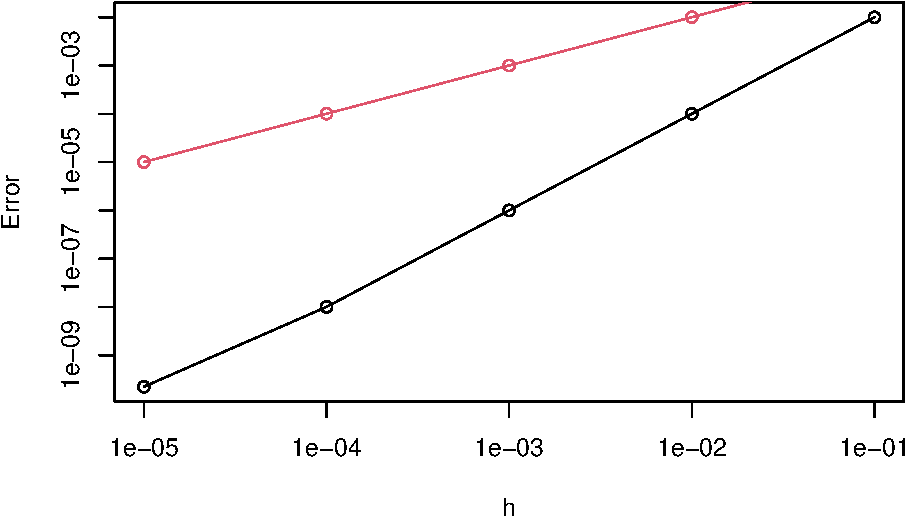
\includegraphics{04-pca_files/figure-latex/unnamed-chunk-10-1.pdf}

R also has a built-in function for doing PCA.

\begin{Shaded}
\begin{Highlighting}[]
\NormalTok{pca <-}\StringTok{ }\KeywordTok{prcomp}\NormalTok{(secondyr[,}\DecValTok{2}\OperatorTok{:}\DecValTok{3}\NormalTok{]) }\CommentTok{# prcomp will automatocally remove the column mean}
\NormalTok{pca}\OperatorTok{$}\NormalTok{rotation }\CommentTok{# the loadings}
\end{Highlighting}
\end{Shaded}

\begin{verbatim}
##            PC1        PC2
## PRB -0.6895160 -0.7242705
## STA -0.7242705  0.6895160
\end{verbatim}

\begin{Shaded}
\begin{Highlighting}[]
\NormalTok{pca}\OperatorTok{$}\NormalTok{x }\CommentTok{# the scores}
\end{Highlighting}
\end{Shaded}

\begin{verbatim}
##              PC1        PC2
##  [1,] -19.060674 -7.2588361
##  [2,] -16.233101 -7.1893271
##  [3,] -11.615016  6.3632849
##  [4,]  14.731183 -0.7695824
##  [5,]  23.074883  5.0940904
##  [6,]  14.939710 -9.2523011
##  [7,]  -3.787059  4.4337549
##  [8,] -29.994240  5.9114764
##  [9,]  15.316435  4.1960474
## [10,]  12.627880 -1.5286074
\end{verbatim}

```

Note that the new variables have sample mean \(\bar{\boldsymbol y}=\boldsymbol 0\). The sample covariance matrix is a diagonal with entries given by the eigenvalues (see part 4. of Proposition \ref{prp:pca1}). Note that there is always some numerical error (so quantities are never 0, and instead are just very small numnbers).

\[
\boldsymbol \Lambda= \text{diag}(\lambda_1,\lambda_2) =  \begin{pmatrix} \lambda_1 & 0 \\ 0 & \lambda_2 \end{pmatrix}.
\]

\begin{Shaded}
\begin{Highlighting}[]
\KeywordTok{colMeans}\NormalTok{(pca}\OperatorTok{$}\NormalTok{x)}
\end{Highlighting}
\end{Shaded}

\begin{verbatim}
##           PC1           PC2 
##  2.842171e-15 -9.769963e-16
\end{verbatim}

\begin{Shaded}
\begin{Highlighting}[]
\KeywordTok{cov}\NormalTok{(pca}\OperatorTok{$}\NormalTok{x)}\OperatorTok{*}\DecValTok{9}\OperatorTok{/}\DecValTok{10} \CommentTok{# to convert to using 1/n as the denominator }
\end{Highlighting}
\end{Shaded}

\begin{verbatim}
##              PC1          PC2
## PC1 3.042437e+02 1.974167e-14
## PC2 1.974167e-14 3.315628e+01
\end{verbatim}

Finally, note that we did the singular value decomposition for \(\boldsymbol X\) above not \(\frac{1}{\sqrt{10}}\boldsymbol X\), and so we'd need to square and scale the singular values to find the eigenvalues. Let's check:

\begin{Shaded}
\begin{Highlighting}[]
\NormalTok{X_svd}\OperatorTok{$}\NormalTok{d}\OperatorTok{^}\DecValTok{2}\OperatorTok{/}\DecValTok{10} \CommentTok{# square and scale the singular values}
\end{Highlighting}
\end{Shaded}

\begin{verbatim}
## [1] 304.24372  33.15628
\end{verbatim}

\begin{Shaded}
\begin{Highlighting}[]
\KeywordTok{eigen}\NormalTok{(}\KeywordTok{t}\NormalTok{(X) }\OperatorTok\StringTok{ }\NormalTok{X}\OperatorTok{/}\DecValTok{10}\NormalTok{)}\OperatorTok{$}\NormalTok{values  }\CommentTok{# compute the eigenvalues of the covariance matrix}
\end{Highlighting}
\end{Shaded}

\begin{verbatim}
## [1] 304.24372  33.15628
\end{verbatim}

\begin{Shaded}
\begin{Highlighting}[]
\KeywordTok{svd}\NormalTok{(X}\OperatorTok{/}\KeywordTok{sqrt}\NormalTok{(}\DecValTok{10}\NormalTok{))}\OperatorTok{$}\NormalTok{d}\OperatorTok{^}\DecValTok{2} \CommentTok{# compute the singular values of X/sqrt(10) and square}
\end{Highlighting}
\end{Shaded}

\begin{verbatim}
## [1] 304.24372  33.15628
\end{verbatim}

\hypertarget{example-iris}{%
\subsection{Example: Iris}\label{example-iris}}

In general when using R to do PCA, we don't need to compute the SVD and then do the projections, as there is an R command \texttt{prcomp} that will do it all for us. The \texttt{princomp} will also do PCA, but is less stable than \texttt{prcomp}, and it is recommended that you use \texttt{prcomp} in preference.

Let's do PCA on the iris dataset discussed in Chapter \ref{stat-prelim}. The \texttt{prcomp} returns the square root of the eigenvalues (the standard devaiation of the PC scores), and the PC scores.

\begin{Shaded}
\begin{Highlighting}[]
\NormalTok{iris.pca =}\StringTok{ }\KeywordTok{prcomp}\NormalTok{(iris[,}\DecValTok{1}\OperatorTok{:}\DecValTok{4}\NormalTok{])}
\NormalTok{iris.pca}\OperatorTok{$}\NormalTok{sdev }\CommentTok{# the square root of the eigenvalues}
\end{Highlighting}
\end{Shaded}

\begin{verbatim}
## [1] 2.0562689 0.4926162 0.2796596 0.1543862
\end{verbatim}

\begin{Shaded}
\begin{Highlighting}[]
\KeywordTok{head}\NormalTok{(iris.pca}\OperatorTok{$}\NormalTok{x)  }\CommentTok{#the PC scores}
\end{Highlighting}
\end{Shaded}

\begin{verbatim}
##            PC1        PC2         PC3          PC4
## [1,] -2.684126 -0.3193972  0.02791483  0.002262437
## [2,] -2.714142  0.1770012  0.21046427  0.099026550
## [3,] -2.888991  0.1449494 -0.01790026  0.019968390
## [4,] -2.745343  0.3182990 -0.03155937 -0.075575817
## [5,] -2.728717 -0.3267545 -0.09007924 -0.061258593
## [6,] -2.280860 -0.7413304 -0.16867766 -0.024200858
\end{verbatim}

The PC loadings/eigenvectors can also be accessed, as can the sample mean

\begin{Shaded}
\begin{Highlighting}[]
\NormalTok{iris.pca}\OperatorTok{$}\NormalTok{rotation }\CommentTok{#the eigenvecstors}
\end{Highlighting}
\end{Shaded}

\begin{verbatim}
##                      PC1         PC2         PC3        PC4
## Sepal.Length  0.36138659 -0.65658877  0.58202985  0.3154872
## Sepal.Width  -0.08452251 -0.73016143 -0.59791083 -0.3197231
## Petal.Length  0.85667061  0.17337266 -0.07623608 -0.4798390
## Petal.Width   0.35828920  0.07548102 -0.54583143  0.7536574
\end{verbatim}

\begin{Shaded}
\begin{Highlighting}[]
\NormalTok{iris.pca}\OperatorTok{$}\NormalTok{center }\CommentTok{# the sample mean of the data}
\end{Highlighting}
\end{Shaded}

\begin{verbatim}
## Sepal.Length  Sepal.Width Petal.Length  Petal.Width 
##     5.843333     3.057333     3.758000     1.199333
\end{verbatim}

A scree plot can be obtained simply by using the \texttt{plot} command. The summary command also gives useful information about the importance of each PC.

\begin{Shaded}
\begin{Highlighting}[]
\KeywordTok{plot}\NormalTok{(iris.pca)}
\end{Highlighting}
\end{Shaded}

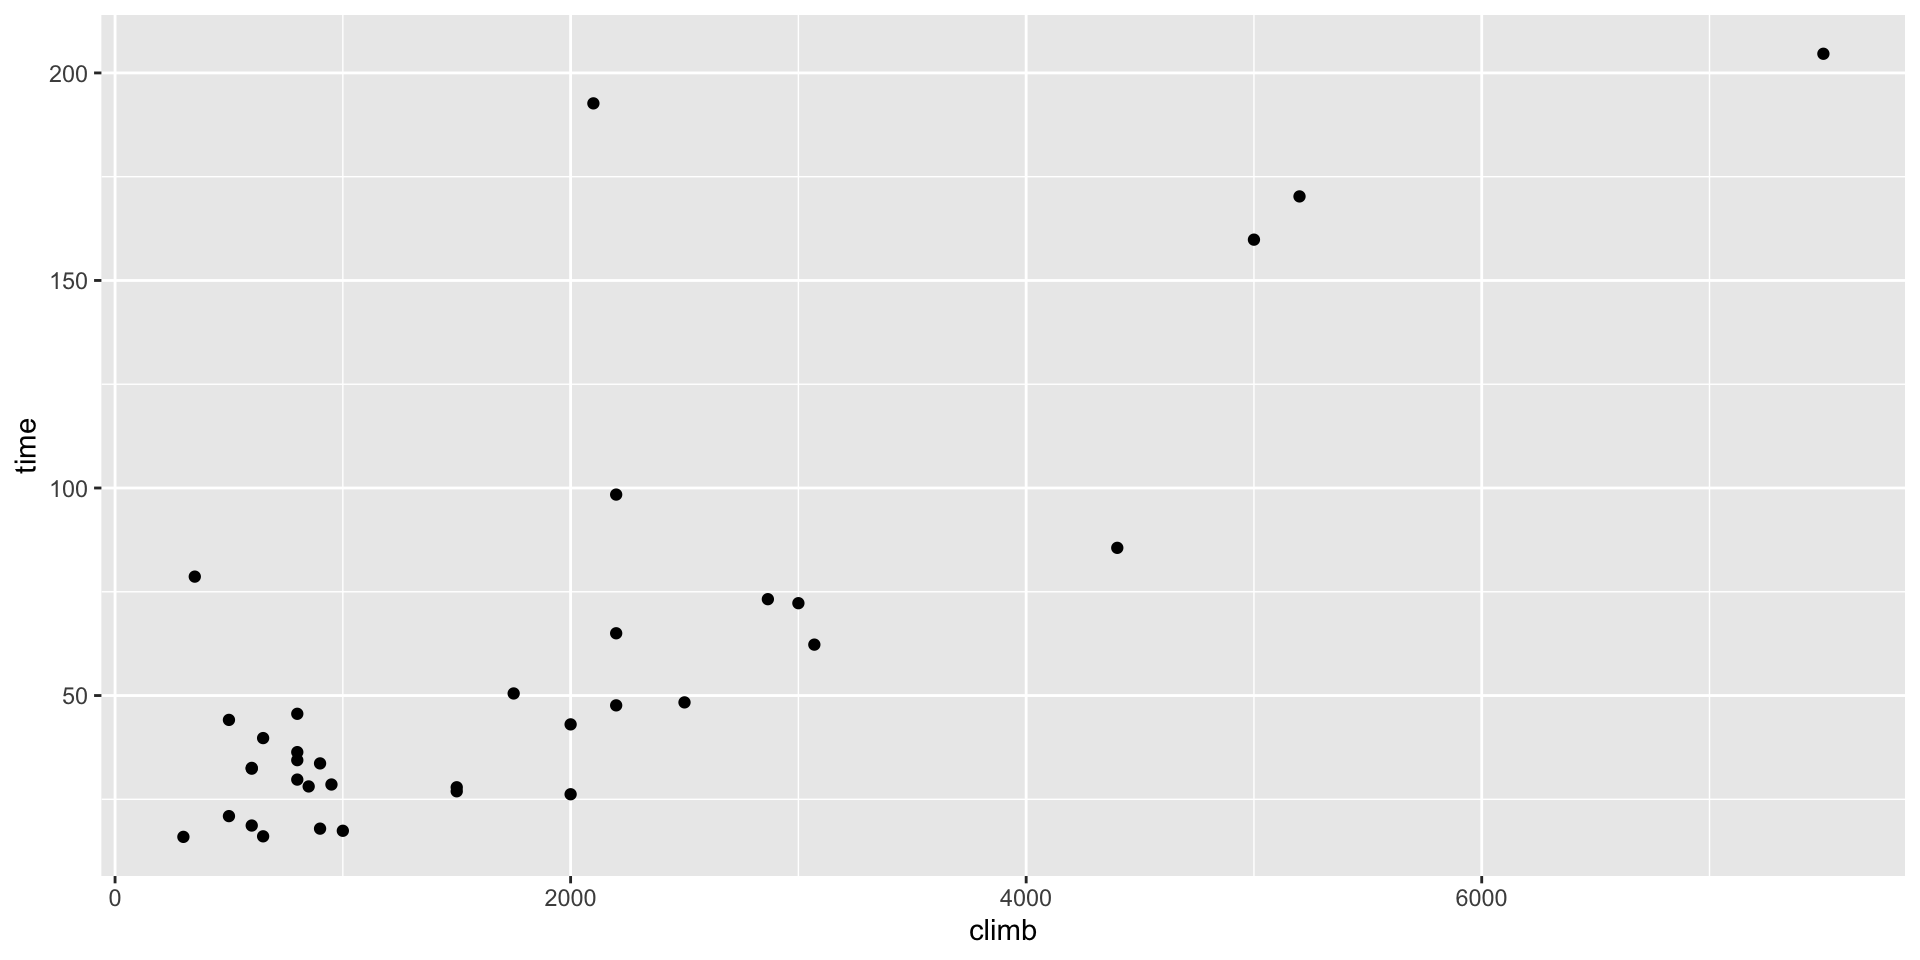
\includegraphics{04-pca_files/figure-latex/unnamed-chunk-16-1.pdf}

\begin{Shaded}
\begin{Highlighting}[]
\KeywordTok{summary}\NormalTok{(iris.pca)}
\end{Highlighting}
\end{Shaded}

\begin{verbatim}
## Importance of components:
##                           PC1     PC2    PC3     PC4
## Standard deviation     2.0563 0.49262 0.2797 0.15439
## Proportion of Variance 0.9246 0.05307 0.0171 0.00521
## Cumulative Proportion  0.9246 0.97769 0.9948 1.00000
\end{verbatim}

To plot the PC scores, you can either manually create a plot or use the \texttt{ggfortify} package. For example, here is a plot of the first two PC scores coloured according to the species of iris.

\begin{Shaded}
\begin{Highlighting}[]
\NormalTok{iris}\OperatorTok{$}\NormalTok{PC1=iris.pca}\OperatorTok{$}\NormalTok{x[,}\DecValTok{1}\NormalTok{]}
\NormalTok{iris}\OperatorTok{$}\NormalTok{PC2=iris.pca}\OperatorTok{$}\NormalTok{x[,}\DecValTok{2}\NormalTok{]}
\KeywordTok{qplot}\NormalTok{(PC1, PC2, }\DataTypeTok{colour=}\NormalTok{Species, }\DataTypeTok{data=}\NormalTok{iris)}
\end{Highlighting}
\end{Shaded}

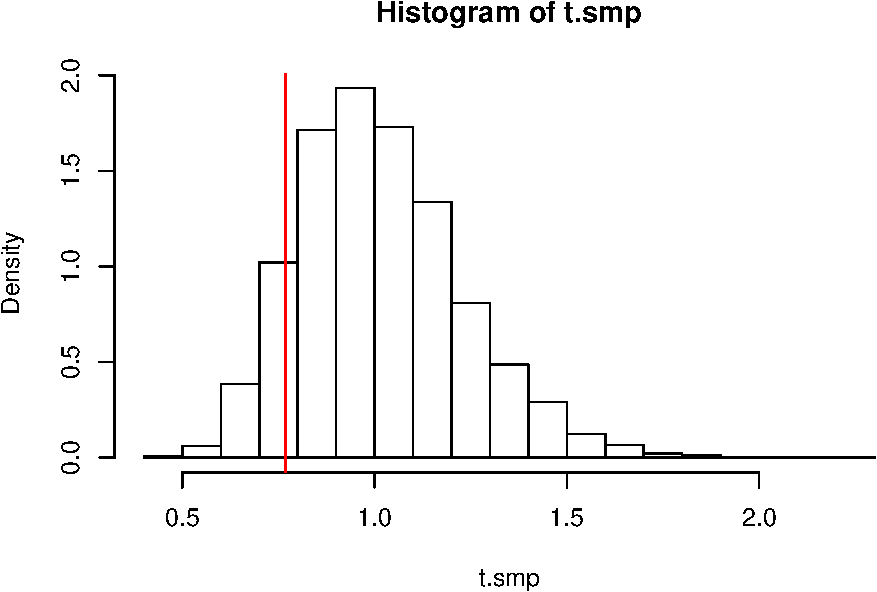
\includegraphics{04-pca_files/figure-latex/unnamed-chunk-17-1.pdf}

The \texttt{ggfortify} package provides a nice wrapper for some of this functionality.

\begin{Shaded}
\begin{Highlighting}[]
\KeywordTok{library}\NormalTok{(ggfortify)}
\KeywordTok{autoplot}\NormalTok{(iris.pca, }\DataTypeTok{data =}\NormalTok{ iris, }\DataTypeTok{colour =} \StringTok{'Species'}\NormalTok{)}
\end{Highlighting}
\end{Shaded}

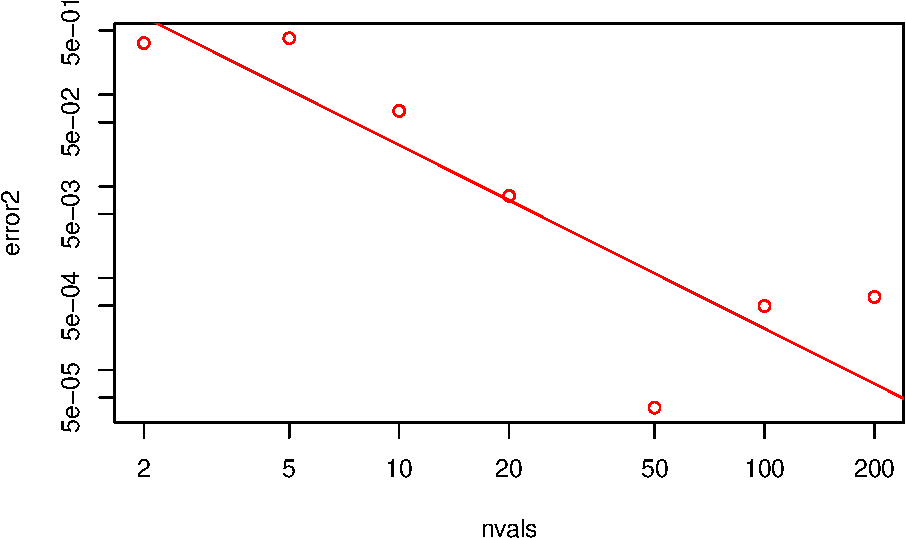
\includegraphics{04-pca_files/figure-latex/unnamed-chunk-18-1.pdf}

\hypertarget{pca-a-formal-description-with-proofs}{%
\section{PCA: a formal description with proofs}\label{pca-a-formal-description-with-proofs}}

Let's now summarize what we've said so far and prove some results about principal component analysis.

Let \(\boldsymbol x_1, \ldots , \boldsymbol x_n\) denote a sample of vectors in \(\mathbb{R}^p\) with sample mean vector \(\bar{\boldsymbol x}\) and sample covariance matrix \(\boldsymbol S\). Suppose \(\boldsymbol S=\boldsymbol X^\top \boldsymbol H\boldsymbol X\) has spectral decomposition (see Proposition \ref{prp:spectraldecomp})
\begin{equation}
\boldsymbol S=\boldsymbol V\boldsymbol \Lambda\boldsymbol V^\top = \sum_{j=1}^p  \lambda_j \boldsymbol v_j \boldsymbol v_j^\top,
\label{eq:pcaspect}
\end{equation}
where the eigenvalues are \(\lambda_1 \geq \lambda_2 \geq \lambda_p \geq 0\) with \(\boldsymbol \Lambda=\text{diag}\{\lambda_1, \ldots, \lambda_p\}\), and \(\boldsymbol V\) contains the eigenvectors of \(\boldsymbol S\).

The principal components of \(\boldsymbol X\) are defined sequentially. The \(j^{th}\) principal component is the solution to the following optimization problem:
\begin{equation}
\max_{\boldsymbol u: \, \vert \vert \boldsymbol u\vert \vert =1}\boldsymbol u^\top \boldsymbol S\boldsymbol u
\label{eq:pcmaxgen}
\end{equation}
subject to
\begin{equation}
\boldsymbol v_k^\top \boldsymbol u=0, \qquad k=1, \ldots , j-1.
\label{eq:pccongen}
\end{equation}
(for \(j=1\) there is no orthogonality constraint).

\begin{proposition}
\protect\hypertarget{prp:pca1}{}{\label{prp:pca1} }The maximum of Equation \eqref{eq:pcmaxgen}
subject to Equation \eqref{eq:pccongen} is equal to \(\lambda_j\) and is obtained when \(\boldsymbol u=\boldsymbol v_j\).
\end{proposition}

\begin{proof}
\iffalse{} {Proof. } \fi{}We can prove this using the method of Lagrange multipliers. For \(j=1\) our objective is
\[\mathcal{L} = \boldsymbol u^\top  \boldsymbol S\boldsymbol u+\lambda(1-\boldsymbol u^\top \boldsymbol u)\]
Differentiating (see \ref{vectordiff}) with respect to \(\boldsymbol u\) and setting the derivative equal to zero gives
\[2\boldsymbol S\boldsymbol u-2\lambda \boldsymbol u=0\]
Rearranging we see that \(\boldsymbol u\) must satify
\[\boldsymbol S\boldsymbol u=\lambda \boldsymbol u\mbox{ with } \boldsymbol u^\top \boldsymbol u=1\]
i.e., \(\boldsymbol u\) is a unit eigenvector of \(\boldsymbol S\). Substituting this back in to the objective we see
\[\boldsymbol u\boldsymbol S\boldsymbol u= \lambda\]
and so we must choose \(\boldsymbol u=\boldsymbol v_1\), the eigenvector corresponding to the largest eigenvalue of \(\boldsymbol S\).

We now proceed inductively and assume the result is true for \(k=1, \ldots, j-1\). The Lagrangian for the \(j^{th}\) optimization problem is
\[\mathcal{L} = \boldsymbol u^\top  \boldsymbol S\boldsymbol u+\lambda(1-\boldsymbol u^\top \boldsymbol u) +\sum_{k=1}^{j-1}\mu_k (1-\boldsymbol u^\top \boldsymbol v_k)\]
where we now have \(j\) Lagrange multipliers \(\lambda, \mu_1, \ldots, \mu_{j-1}\) - one for each constraint.
Differentiating with respect to \(\boldsymbol u\) and setting equal to zero gives
\[0 = 2\boldsymbol S\boldsymbol u- 2\lambda \boldsymbol u- \sum_{k=1}^{j-1} \mu_k\boldsymbol v_k=0 \]
If we left multiply by \(\boldsymbol v_l\) we get
\[2\boldsymbol v_l^\top \boldsymbol S\boldsymbol u- \lambda \boldsymbol v_l \boldsymbol u- \sum \mu_k \boldsymbol v_l^\top \boldsymbol v_k =0\]
We know \(\boldsymbol v_l\) is an eigenvector of \(\boldsymbol S\) and so \(\boldsymbol S\boldsymbol v_l=\lambda_l \boldsymbol v_l\) and hence \(\boldsymbol v_k \boldsymbol S\boldsymbol u=0\) as \(\boldsymbol v_l^\top \boldsymbol u=0\). Also \[\boldsymbol v_l^\top\boldsymbol v_k=\begin{cases}1 &\mbox{ if } k=l\\
0 &\mbox{ otherwise, }\end{cases}\] and thus we've shown that \(\mu_l=0\) for \(l=1, \ldots, j-1\). So again we have that \[\boldsymbol S\boldsymbol u= \lambda \boldsymbol u\]
i.e., \(\boldsymbol u\) must be a unit eigenvector of \(\boldsymbol S\). It only remains to show \emph{which} eigenvector it is. Because \(\boldsymbol u\) must be orthogonal to \(\boldsymbol v_1, \ldots, \boldsymbol v_{j-1}\),
and as \(\boldsymbol v_l^\top \boldsymbol S\boldsymbol v_l = \lambda_l\), we must choose \(\boldsymbol u=\boldsymbol v_j\), the eigenvector corresponding to the \(j^{th}\) largest eigenvalue.
\end{proof}

\hypertarget{properties-of-principal-components}{%
\subsection{Properties of principal components}\label{properties-of-principal-components}}

For \(j=1, \ldots , p\), the scores of the \(j^{th}\) principal component (PC) are given by
\[
y_{ij}=\boldsymbol v_j^\top(\boldsymbol x_i - \bar{\boldsymbol x}), \qquad i=1, \ldots , n.
\]
The \(j^{th}\) eigenvector \(\boldsymbol v_j\) is sometimes referred to as the vector of \textbf{loadings} for the \(j^{th}\) PC.

In vector notation
\[
\boldsymbol y_i=( y_{i1}, y_{i2}, \ldots , y_{ip})^\top = \boldsymbol V^\top (\boldsymbol x_i -\bar{\boldsymbol x}), \qquad i=1, \ldots ,n.
\]
In matrix form, the full set of PC scores is given by
\[
\boldsymbol Y= [\boldsymbol y_1 , \ldots , \boldsymbol y_n]^\top =\boldsymbol H\boldsymbol X\boldsymbol V.
\]

If \(\tilde{\boldsymbol X}=\boldsymbol H\boldsymbol X\) is the column centered data matrix, with singular value decomposition
\(\tilde{\boldsymbol X}=\boldsymbol U\boldsymbol \Sigma\boldsymbol V^\top\) with \(\boldsymbol V\) as in Equation \eqref{eq:pcaspect}, then
\[\boldsymbol Y= \tilde{\boldsymbol X}\boldsymbol V= \boldsymbol U\boldsymbol \Sigma.\]

The transformed variables \(\boldsymbol y= \boldsymbol H\boldsymbol X\boldsymbol V\) have some important properties which we collect together in the following proposition.

\begin{proposition}
\protect\hypertarget{prp:pca2}{}{\label{prp:pca2} }The following results hold:

\begin{enumerate}
\def\labelenumi{\arabic{enumi}.}
\item
  The sample mean vector of \(\boldsymbol y_1, \ldots , \boldsymbol y_n\) is the zero vector: \(\bar{\boldsymbol y}={\mathbf 0}_p\)
\item
  The sample covariance matrix of \(\boldsymbol y_1, \ldots, \boldsymbol y_n\) is
  \[\Lambda = \operatorname{diag}(\lambda_1, \ldots, \lambda_p)\]
  i.e., for each fixed \(j\), the sample variance of \(y_{ij}\) is \(\lambda_j\), and \(y_{ij}\) is uncorrelated with with \(y_{ik}\) for \(j\not = k\).
\item
  For \(j\leq k\) the sample variance of \(\{y_{ij}\}_{i=1, \ldots , n}\) is greater than or equal to the sample variance of \(\{y_{ik}\}_{i=1, \ldots , n}\).
  \[\boldsymbol q_1^\top \boldsymbol S\boldsymbol q_1 \geq \boldsymbol q_2^\top \boldsymbol S\boldsymbol q_2 \geq \ldots \geq \boldsymbol q_p^\top \boldsymbol S\boldsymbol q_p\geq 0\]
\item
  The sum of the sample variances is equal to the trace of \(\boldsymbol S\)
  \[\sum_{j=1}^p \boldsymbol q_j^\top \boldsymbol S\boldsymbol q_j = \sum_{j=1}^p \lambda_j = \text{tr}(\boldsymbol S)\]
\item
  The product of the sample variances is equal to the determinant of \(\boldsymbol S\)
  \[\prod_{j=1}^p \boldsymbol q_j^\top \boldsymbol S\boldsymbol q_j = \prod_{j=1}^p \lambda_j = |\boldsymbol S|.\]
\end{enumerate}
\end{proposition}

\begin{proof}
\iffalse{} {Proof. } \fi{}For i.
\[\bar{\boldsymbol y} = \frac{1}{n}\sum_{i=1}^n \boldsymbol V^\top(\boldsymbol x_i-\bar{\boldsymbol x}) = \frac{1}{n} \boldsymbol V^\top\sum_{i=1}^n(\boldsymbol x_i-\bar{\boldsymbol x}) =\boldsymbol 0.\]

For 2. the sample covariance matrix of \(\boldsymbol y_1, \ldots, \boldsymbol y_n\) is
\begin{align*}
\frac{1}{n}\sum_{i=1}^n \boldsymbol y_i \boldsymbol y_i^\top &=\frac{1}{n} \sum \boldsymbol V^\top (\boldsymbol x_i-\bar{\boldsymbol x})(\boldsymbol x_i - \boldsymbol x)^\top \boldsymbol V\\
&=\boldsymbol V^\top \boldsymbol S\boldsymbol V\\
&=\boldsymbol V^\top \boldsymbol V\boldsymbol \Lambda\boldsymbol V^\top \boldsymbol V\mbox{ substiting the spectral decomposition for }\boldsymbol S\\
&=\boldsymbol \Lambda
\end{align*}

\begin{enumerate}
\def\labelenumi{\arabic{enumi}.}
\setcounter{enumi}{2}
\item
  is a consequence 2. and of ordering the eigenvalues in decreasing magnitude.
\item
  follows from lemma \ref{lem:trace} and the spectral decomposition of \(\boldsymbol S\):
  \[\operatorname{tr}(\boldsymbol S) = \operatorname{tr}(\boldsymbol V\boldsymbol \Lambda\boldsymbol V^\top)  =\operatorname{tr}(\boldsymbol V^\top \boldsymbol V\boldsymbol \Lambda)=\operatorname{tr}(\boldsymbol \Lambda)=\sum\lambda_i\]
\item
  follows from \ref{prp:deteig}.
\end{enumerate}
\end{proof}

From these properties we say that a proportion
\[\frac{\lambda_j}{\lambda_1 + \ldots + \lambda_p}\]
of the variability in the sample is `explained' by the \(j^{th}\) PC.

One tool for looking at the contributions of each PC is to look at the \textbf{scree plot} which plots the percentage of variance explained by PC \(j\) against \(j\). We'll see examples of scree plots below.

\hypertarget{example-football}{%
\subsection{Example: Football}\label{example-football}}

We can apply PCA to a football league table where \(W\), \(D\), \(L\) are the number of matches won, drawn and lost and \(G\) and \(GA\) are the goals scored for and against, and \(GD\) is the goal difference (\(G-GA\)). An extract of the table for a recent Premiership season is:

\begin{tabular}{lrrrrrr}
\toprule
Team & W & D & L & G & GA & GD\\
\midrule
Liverpool & 32 & 3 & 3 & 85 & 33 & 52\\
Manchester City & 26 & 3 & 9 & 102 & 35 & 67\\
Manchester United & 18 & 12 & 8 & 66 & 36 & 30\\
Chelsea & 20 & 6 & 12 & 69 & 54 & 15\\
Leicester City & 18 & 8 & 12 & 67 & 41 & 26\\
\addlinespace
Tottenham Hotspur & 16 & 11 & 11 & 61 & 47 & 14\\
Wolverhampton & 15 & 14 & 9 & 51 & 40 & 11\\
Arsenal & 14 & 14 & 10 & 56 & 48 & 8\\
Sheffield United & 14 & 12 & 12 & 39 & 39 & 0\\
Burnley & 15 & 9 & 14 & 43 & 50 & -7\\
\bottomrule
\end{tabular}

The sample mean vector is

\[\bar{\boldsymbol x} =\begin{pmatrix}14.4 \\9.2 \\14.4 \\51.7 \\51.7 \\0 \\\end{pmatrix}.\]

Note that the total goals scored must equal the total goals conceded, and that the sum of the goal differences must be \(0\). The sample covariance matrix is

\begin{equation}
\boldsymbol S= \begin{pmatrix}38.3&-9.18&-29.2&103&-57&160 \\-9.18&10.2&-0.98&-27.5&-2.24&-25.2 \\-29.2&-0.98&30.1&-75.3&59.3&-135 \\103&-27.5&-75.3&336&-147&483 \\-57&-2.24&59.3&-147&134&-281 \\160&-25.2&-135&483&-281&764 \\\end{pmatrix}
\label{eq:PLES}
\end{equation}

The eigenvalues of \(\boldsymbol S\) are
\[\boldsymbol \Lambda= \text{diag}\begin{pmatrix}1300&71.9&8.05&4.62&-2.65e-14&-3.73e-14 \\\end{pmatrix}\]

Note that we have two zero eigenvalues (which won't be computed as exactly zero because of numerical rounding errors) because two of our variables are a linear combinations of the other variables, \(W+D+L = 38\) and \(GD=G-GA\). The corresponding eigenvectors are
\[\boldsymbol V= [\boldsymbol v_1 \ldots \boldsymbol v_6] =\begin{pmatrix}0.166&-0.0262&0.707&0.373&-0.577&0 \\-0.0282&0.275&-0.661&0.391&-0.577&1.06e-14 \\-0.138&-0.249&-0.0455&-0.764&-0.577&-2.04e-14 \\0.502&-0.6&-0.202&0.117&3.22e-15&-0.577 \\-0.285&-0.701&-0.11&0.286&-6.11e-15&0.577 \\0.787&0.101&-0.0915&-0.169&-3.33e-16&0.577 \\\end{pmatrix}\]

The proportion of variability explained by each of the PCs is:
\[
\begin{pmatrix}0.939&0.052&0.00583&0.00334&-1.92e-17&-2.7e-17 \\\end{pmatrix}
\]

There is no point computing the scores for PC 5 and 6, because these do not explain any of the variability in the data. Similarly, there is little value in computing the scores for PCs 3 \& 4 because they account for less than 1\% of the variability in the data.

We can, therefore, choose to compute only the first two PC scores. We are reducing the dimension of our data set from \(p=5\) to \(p=2\) while still retaining 99\% of the variability. The first PC score/transformed variable is given by:
\begin{align*}
y_{i1} &= 0.17(W_i-\bar{W}) +-0.03(D_i-\bar{D}) +-0.14(L_i-\bar{L})\\
& \qquad +0.5(G_i-\bar{G}) +-0.28(GA_i-\bar{GA})+0.79(GD_i-\bar{GD}),
\end{align*}
and similarly for PC 2.

The first five rows of our revised ``league table'' are now

\begin{table}[H]
\centering
\begin{tabular}{lrr}
\toprule
Team & PC1 & PC2\\
\midrule
Liverpool & -67.6 & 0.9\\
Manchester City & -85.6 & 12.3\\
Manchester United & -36.7 & -7.7\\
Chelsea & -21.2 & 10.9\\
Leicester City & -32.2 & -1.1\\
\bottomrule
\end{tabular}
\end{table}

Now that we have reduced the dimension to \(p=2\), we can visualise the differences between the teams.
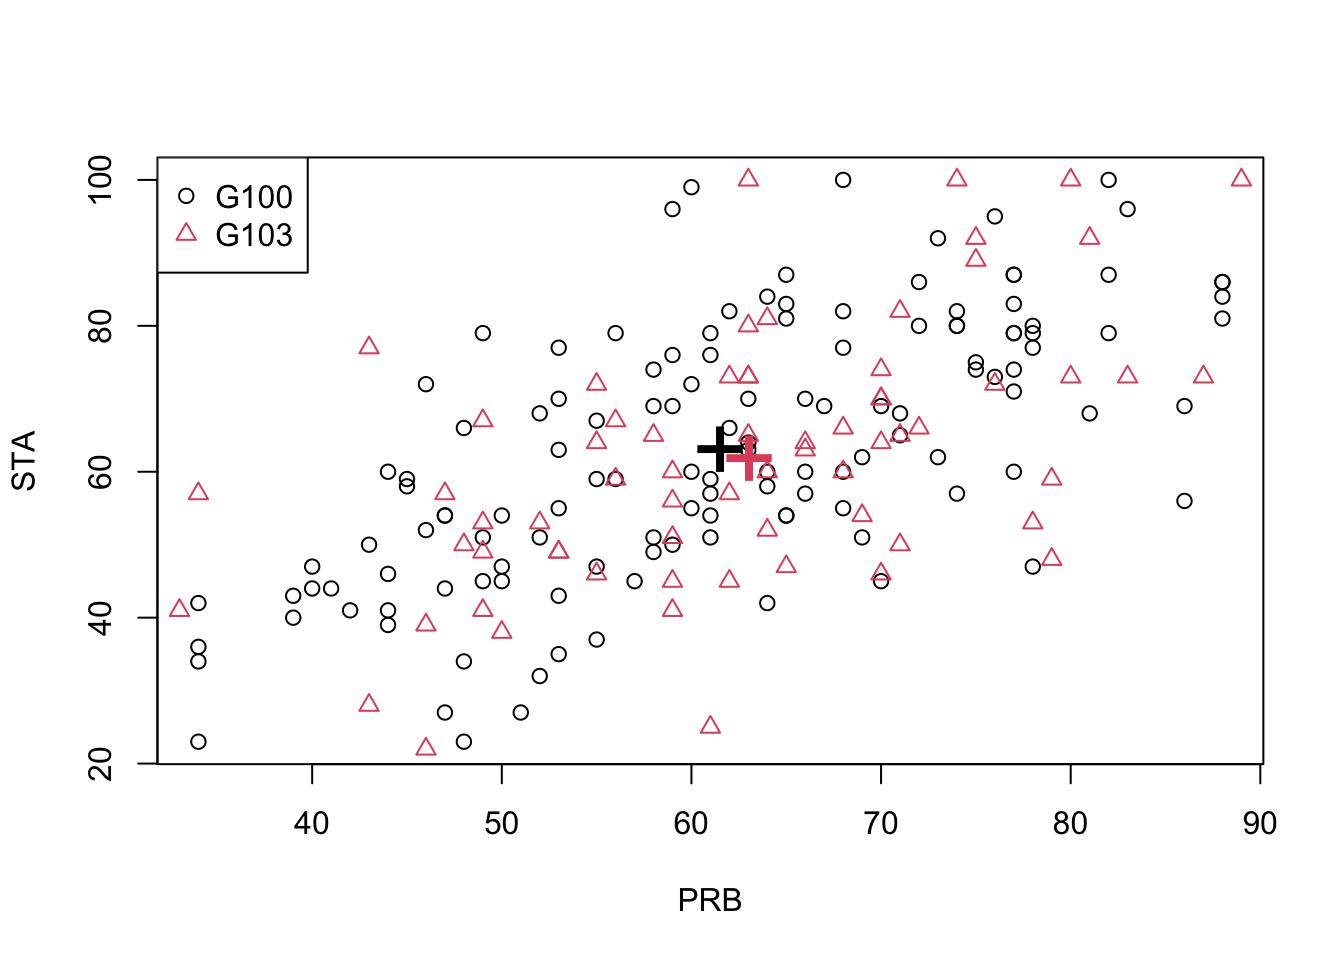
\includegraphics{04-pca_files/figure-latex/unnamed-chunk-26-1.pdf}

We might interpret the PCs as follows. The first PC seems to measure the difference in goals scored and conceded between teams. It rewards teams with 0 for positive goal difference, and 0.37 for each goal scored, whilst penalising them by -0.58 for every goal they concede. So a team with a large positive PC1 score tends to score lots of goals and concede few. If we rank teams by their PC1 score, and compare this with the rankings using 3 points for a win and 1 point for a draw we get a different ranking of the teams.

\begin{tabular}{lrr}
\toprule
  & PC1 & PC2\\
\midrule
Liverpool & -67.637127 & 0.9306615\\
Manchester City & -85.593967 & 12.3492387\\
Manchester United & -36.661797 & -7.7344979\\
Chelsea & -21.190382 & 10.9021516\\
Leicester City & -32.155292 & -1.1285032\\
\addlinespace
Tottenham Hotspur & -17.710519 & -0.4325749\\
Wolverhampton & -12.342929 & -12.3850152\\
Arsenal & -9.913433 & -3.2498502\\
Sheffield United & 2.580462 & -17.9013025\\
Burnley & 9.235955 & -5.7314925\\
\bottomrule
\end{tabular}

The second PC has a strong negative loading for both goals for and against. A team with a large negative PC 2 score was, therefore, involved in matches with lots of goals. We could, therefore, interpret PC 2 as an `'entertainment'' measure, ranking teams according to their involvement in high-scoring games.

The above example raises the question of how many PCs should we use in practice. If we reduce the dimension to \(p=1\) then we can rank observations and analyse our new variable with univariate statistics. If we reduce the dimension to \(p=2\) then it is still easy to visualise the data. However, reducing the dimension to \(p=1\) or \(p=2\) may involve losing lots of information and a sensible answer should depend on the objectives of the analysis and the data itself.

The scree graph for the football example is:

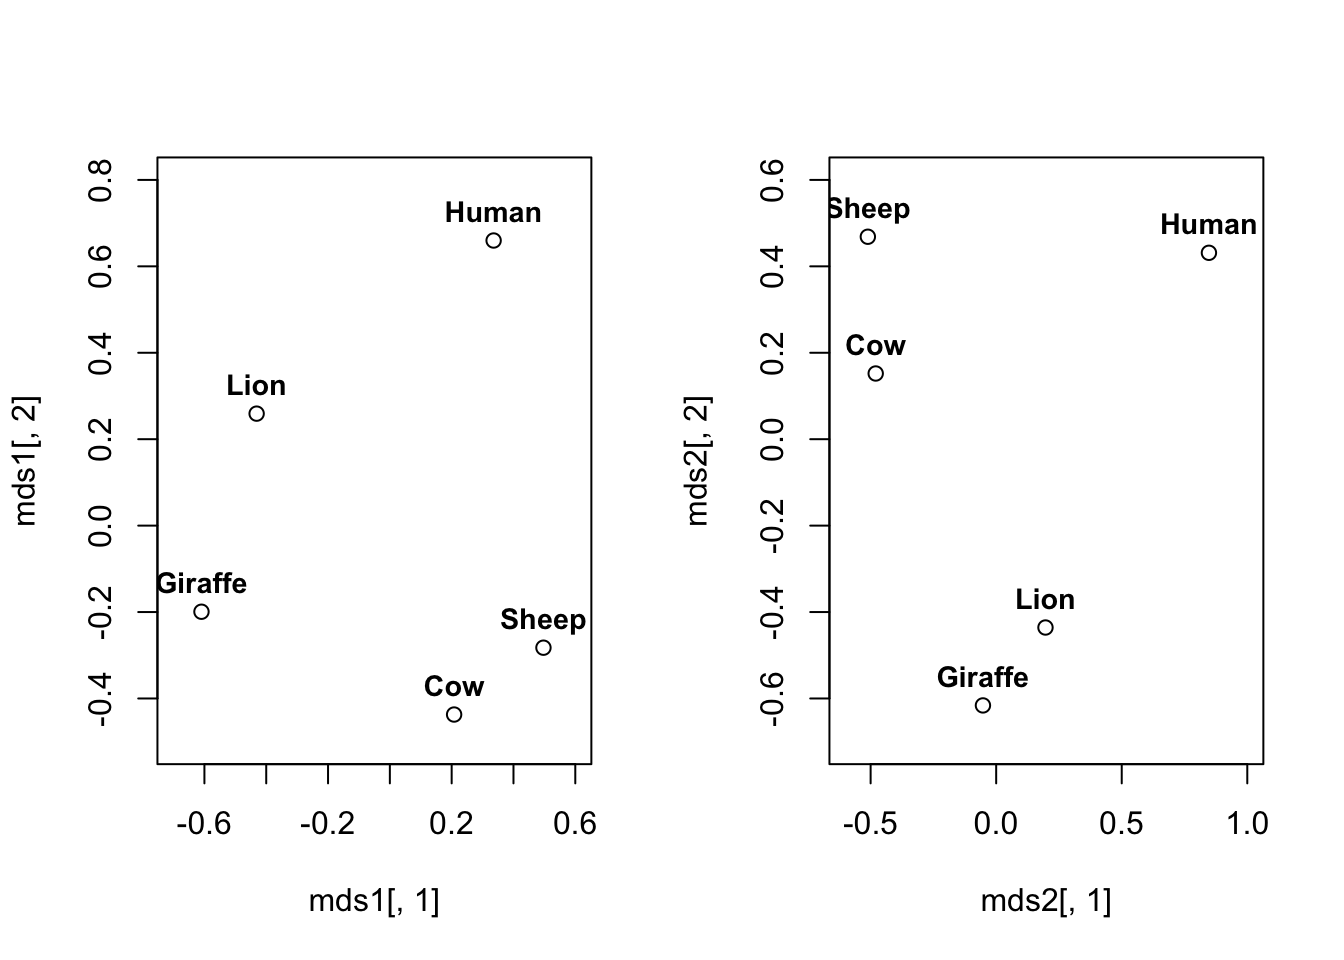
\includegraphics{04-pca_files/figure-latex/unnamed-chunk-29-1.pdf}
There are many possible methods for choosing the number of PCs to retain for analysis, including:

\begin{itemize}
\tightlist
\item
  retaining enough PCs to explain, say, 90\% of the total variation;
\item
  retaining PCs where the eigenvalue is above the average.
\end{itemize}

To retain enough PCs to explain 90\% of the total variance, would require us to keep just a single PCs in this case.

\hypertarget{pcawithR}{%
\subsection{\texorpdfstring{PCA based on \(\boldsymbol R\) versus PCA based on \(\boldsymbol S\)}{PCA based on \textbackslash{}boldsymbol R versus PCA based on \textbackslash{}boldsymbol S}}\label{pcawithR}}

Recall the distinction between the sample covariance matrix \(\boldsymbol S\) and the sample correlation matrix \(\boldsymbol R\).
Note that all correlation matrices are also covariance matrices, but not all covariance matrices are correlation matrices.
Before doing PCA we must decide whether to do PCA based on \(\boldsymbol S\) or \(\boldsymbol R\)? As we will see later

\begin{itemize}
\tightlist
\item
  PCA based on \(\boldsymbol R\) (but not \(\boldsymbol S\)) is scale invariant, whereas
\item
  PCA based on \(\boldsymbol S\) is invariant under orthogonal rotation.
\end{itemize}

If the original \(p\) variables represent very different types of quantity or show marked differences in variances, then it will usually be better to use \(\boldsymbol R\) rather than \(\boldsymbol S\). However, in some circumstances, we may wish to use \(\boldsymbol S\), such as when the \(p\) variables are measuring similar entities and the sample variances are not too different.

Given that the required numerical calculations are easy to perform in R, we might wish to do it both ways and see if it makes much difference. To use the correlation matrix \(\boldsymbol R\), we just add the option \texttt{scale=TRUE} when using the \texttt{prcomp} command.

\hypertarget{football-example-continued}{%
\subsubsection{Football example continued}\label{football-example-continued}}

If we repeat the analysis of the football data using \(\boldsymbol R\) instead of \(\boldsymbol S\), we get find principal components:

\begin{align*}
\boldsymbol \Lambda&= \text{diag}\begin{pmatrix}4.51&1.25&0.156&0.0863&3.68e-32&2.48e-33 \\\end{pmatrix}\\
\;\\
\boldsymbol V= [\boldsymbol v_1 \ldots \boldsymbol v_6] &=\begin{pmatrix}-0.456&0.149&-0.342&-0.406&0.466&0.52 \\0.143&-0.844&0.344&-0.143&0.24&0.268 \\0.432&0.321&0.186&0.541&0.413&0.461 \\-0.438&0.214&0.7&-0.0181&0.389&-0.348 \\0.419&0.342&0.386&-0.671&-0.245&0.22 \\-0.466&-0.00136&0.302&0.269&-0.586&0.525 \\\end{pmatrix}
\end{align*}

The effect of using \(\boldsymbol R\) is to standardize each of the original variables to have variance 1.
The first PC now has loadings which are more evenly balanced across the 6 original variables.

Teams will have a small value of PC1 score if they won lots, lost rarely, scored a lot, and conceded rarely. In other words, PC1 is a complete measure of overall performance. If we look at the league table based on ordering according to PC1 we get a table that looks more like the original table.

\begin{tabular}{lrr}
\toprule
  & PC1 & PC2\\
\midrule
Liverpool & -4.6996438 & 1.2003675\\
Manchester City & -4.3806921 & 1.6517491\\
Manchester United & -2.0067554 & -1.2938783\\
Chelsea & -1.2946867 & 1.0826790\\
Leicester City & -1.6563468 & 0.1216950\\
\addlinespace
Tottenham Hotspur & -0.9093467 & -0.6509021\\
Wolverhampton & -0.8242372 & -1.8777265\\
Arsenal & -0.4606630 & -1.5565564\\
Sheffield United & -0.1849220 & -1.3791244\\
Burnley & 0.1752204 & -0.1047675\\
\bottomrule
\end{tabular}

Overall for these data, doing PCA with \(\boldsymbol R\) instead of \(\boldsymbol S\) better summarizes the data (although this is just my subjective opinion - you may feel differently).

\begin{Shaded}
\begin{Highlighting}[]
\KeywordTok{library}\NormalTok{(ggfortify)}
\KeywordTok{autoplot}\NormalTok{(prem.pca, }\DataTypeTok{data =}\NormalTok{ table,  }\DataTypeTok{label =} \OtherTok{TRUE}\NormalTok{,  }\DataTypeTok{label.size =} \DecValTok{3}\NormalTok{, }\DataTypeTok{shape=}\OtherTok{FALSE}\NormalTok{)}
\end{Highlighting}
\end{Shaded}

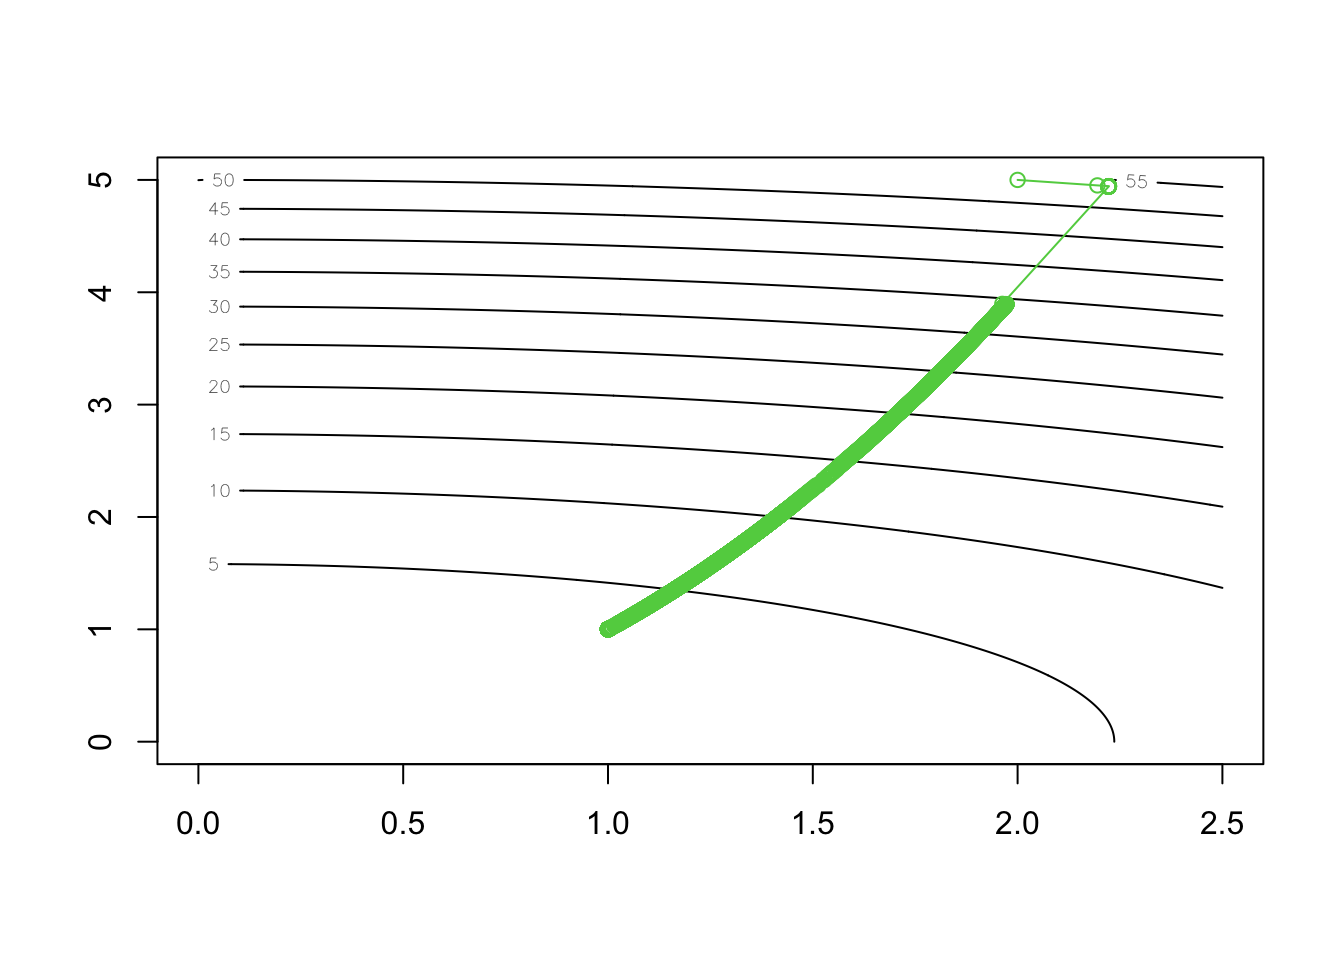
\includegraphics{04-pca_files/figure-latex/unnamed-chunk-32-1.pdf}

\hypertarget{population-pca}{%
\subsection{Population PCA}\label{population-pca}}

So far we have considered sample PCA based on the sample covariance matrix or sample correlation matrix:
\[
\boldsymbol S=\frac{1}{n}\sum_{i=1}^n (\boldsymbol x_i-\bar{\boldsymbol x})(\boldsymbol x_i-\bar{\boldsymbol x})^\top.
\]

We note now that there is a \emph{population} analogue of PCA based on the population
covariance matrix \(\boldsymbol \Sigma\). Although the population version of PCA is not of as much direct practical
relevance as sample PCA, it is nevertheless of conceptual importance.

Let \(\boldsymbol x\) denote a \(p \times 1\) random vector with \({\mathbb{E}}(\boldsymbol x)={\pmb \mu}\) and \({\mathbb{V}\operatorname{ar}}(\boldsymbol x)={\pmb \Sigma}\). As defined,
\(\pmb \mu\) is the population mean vector and \(\pmb \Sigma\) is the population covariance matrix.

Since \(\pmb \Sigma\) is symmetric, the spectral decomposition theorem tells us that
\[
{\pmb \Sigma}=\sum_{j=1}^p \check{\lambda}_j \check{\boldsymbol v}_j \check{\boldsymbol v}_j^\top=\check{\boldsymbol V} \check{\boldsymbol \Lambda}\check{\boldsymbol V}^\top
\]
where the `check' symbol \(\quad \check{} \quad\) is used to distinguish population quantities from their sample analogues.

Then:

\begin{itemize}
\tightlist
\item
  the first population PC is defined by \(Y_1=\check{\boldsymbol v}_1^\top (\boldsymbol x-{\pmb \mu})\);
\item
  the second population PC is defined by \(Y_2=\check{\boldsymbol v}_2^\top (\boldsymbol x-{\pmb \mu})\);
\item
  \(\ldots\)
\item
  the \(p\)th population PC is defined by \(Y_p=\check{\boldsymbol v}_p^\top (\boldsymbol x-{\pmb \mu})\).
\end{itemize}

The \(Y_1, \ldots , Y_p\) are random variables, unlike the sample PCA case, where the \(y_{ij}\) are observed quantities.
In the sample PCA case, the \(y_{ij}\) can often be regarded as the observed values of random variables.

In matrix form, the above definitions can be summarised by writing
\[
\boldsymbol y=\begin{pmatrix} Y_1 \\ Y_2 \\ ... \\...\\Y_p   \end{pmatrix} = \check{\boldsymbol V}^\top (\boldsymbol x-{\pmb \mu}).
\]

The population PCA analogues of the sample PCA properties listed in Proposition \ref{prp:pca2} are now given. Note that the
\(Y_j\)'s are random variables as opposed to observed values of random variables.

\begin{proposition}
\protect\hypertarget{prp:pca3}{}{\label{prp:pca3} }The following results hold for the random variables \(Y_1, \ldots , Y_p\) defined above.

\begin{enumerate}
\def\labelenumi{\arabic{enumi}.}
\item
  \({\mathbb{E}}(Y_j)=0\) for \(j=1, \ldots , p\);
\item
  \({\mathbb{V}\operatorname{ar}}(Y_j)=\check{\lambda}_j\) for \(j=1,\ldots, p\);
\item
  \({\mathbb{C}\operatorname{ov}}(Y_j,Y_k)=0\) if \(j \neq k\);
\item
  \({\mathbb{V}\operatorname{ar}}(Y_1) \geq {\mathbb{V}\operatorname{ar}}(Y_2) \geq \cdots \geq {\mathbb{V}\operatorname{ar}}(Y_p) \geq 0\);
\item
  \(\sum_{j=1}^p {\mathbb{V}\operatorname{ar}}(Y_j)=\sum_{j=1}^p \check{\lambda}_j=\text{tr}(\boldsymbol \Sigma)\);
\item
  \(\prod_{j=1}^p \text{Var}(Y_j)=\prod_{j=1}^p \check{\lambda}_j=\vert \boldsymbol \Sigma\vert\).
\end{enumerate}
\end{proposition}

Note that, defining \(\boldsymbol y=(Y_1, \ldots , Y_p)^\top\) as before, part 1. implies that \({\mathbb{E}}(\boldsymbol y)={\mathbf 0}_p\) and parts 2. and 3. together imply that
\[
\text{Var}(\boldsymbol y)=\boldsymbol \Lambda\equiv \text{diag}(\check{\lambda}_1, \ldots , \check{\lambda}_p).
\]

Consider now a repeated sampling framework in which we assume that \(\boldsymbol x_1, \ldots , \boldsymbol x_n\) are IID random vectors from a population
with mean vector \(\pmb \mu\) and covariance matrix \(\boldsymbol \Sigma\).

What is the relationship between the sample PCA based on the sample of observed vectors \(\boldsymbol x_1, \ldots , \boldsymbol x_n\), and the population PCA based on the unobserved random vector \(\boldsymbol x\),
from the same population?

If the elements of \(\boldsymbol \Sigma\) are all finite, then as \(n\) increases, the elements of the sample covariance matrix \(\boldsymbol S\) will converge to the corresponding elements
of the population covariance matrix \(\boldsymbol \Sigma\). Consequently, we expect the principal components from sample PCA to converge to the population PCA values as \(n\) grows large. Justification of this statement comes from the weak law of large numbers applied to the components of \(\Sigma\), but the details are beyond the scope of this module.

\hypertarget{pca-under-transformations-of-variables}{%
\subsection{PCA under transformations of variables}\label{pca-under-transformations-of-variables}}

We'll now consider what happens to PCA when the data are transformed in various ways.

\textbf{Addition transformation}

Firstly, consider the transformation of addition where, for example, we add a fixed amount to each variable.
We can write this transformation as \(\boldsymbol z_i = \boldsymbol x_i + \boldsymbol c\), where \(\boldsymbol c\) is a fixed vector. Under this transformation the sample mean changes, \(\bar{\boldsymbol z} = \bar{\boldsymbol x} + \boldsymbol c\), but the sample variance remains \(\boldsymbol S\). Consequently, the eigenvalues and eigenvectors remain the same and, therefore, so do the principal component scores/transformed vasriables,
\[\boldsymbol y_i = \boldsymbol V^\top (\boldsymbol z_i - \bar{\boldsymbol z}) = \boldsymbol V^\top(\boldsymbol x_i + \boldsymbol c- (\bar{\boldsymbol x} + \boldsymbol c)) = \boldsymbol V^\top (\boldsymbol x_i - \bar{\boldsymbol x}).\]
We say that the principal components are \textbf{invariant} under the addition transformation. An important special case is to choose \(\boldsymbol c= -\bar{\boldsymbol x}\) so that the PC scores are simply \(\boldsymbol y_i = \boldsymbol V^\top \boldsymbol z_i\).

\textbf{Scale transformation}

Secondly, we consider the scale transformation where each variable is multiplied by a fixed amount.
A scale transformation occurs more naturally when we convert units of measurement from, say, metres to kilometres. We can write this transformation as \(\boldsymbol z_i = \boldsymbol D\boldsymbol x_i\), where \(\boldsymbol D\) is a diagonal matrix with positive elements. Under this transformation the sample mean changes from \(\bar{\boldsymbol x}\) to \(\bar{\boldsymbol z} = \boldsymbol D\bar{\boldsymbol x}\), and the sample covariance matrix changes from \(\boldsymbol S\) to \(\boldsymbol D\boldsymbol S\boldsymbol D\). Consequently, the principal components also change.

This lack of scale-invariance is undesirable. For example, if we analysed data that included some information on distances, we don't want the answer to depend upon whether we use km, metres, or miles as the measure of distance.
One solution is to scale the data using
\[
\boldsymbol D= \text{diag}(s_{11}^{-1/2}, \ldots , s_{pp}^{-1/2}),
 \]
where \(s_{ii}\) is the \(i\)th diagonal element of \(\boldsymbol S\). In effect, we have standardised all the new variables to have variance 1. In this case the sample covariance matrix of the \(\boldsymbol z_i\)'s is simply the sample correlation matrix \(\boldsymbol R\) of the original variables, \(\boldsymbol x_i\). Therefore, we can carry out PCA on the sample correlation matrix, \(\boldsymbol R\), which is invariant to changes of scale.

In summary: \(\boldsymbol R\) is scale-invariant while \(\boldsymbol S\) is not. To do PCA on \(\boldsymbol R\) in R we use the option \texttt{scale=TRUE} in the \texttt{prcomp} command.

We saw an example of this in section \ref{pcawithR} with the football data. Because the sample
variances of \(G\) and \(GA\) are much larger than the sample variances of \(W\), \(D\) and \(L\), doing PCA with \(\boldsymbol R\) instead of \(\boldsymbol S\) completely changed the analysis.

\textbf{Orthogonal transformations}

Thirdly, we consider a transformation by an orthogonal matrix, \(\stackrel{p \times p}{\boldsymbol A}\), such that \(\boldsymbol A\boldsymbol A^\top = \boldsymbol A^\top \boldsymbol A= \mathbf I_p\), and write \(\boldsymbol z_i = \boldsymbol A\boldsymbol x_i\). This is equivalent to rotating and/or reflecting the original data.

Let \(\boldsymbol S\) be the sample covariance matrix of the \(\boldsymbol x_i\) and let \(\boldsymbol T\) be the sample covariance matrix of the \(\boldsymbol z_i\). Under this transformation the sample mean changes from \(\bar{\boldsymbol x}\) to \(\bar{\boldsymbol z} = \boldsymbol A\bar{\boldsymbol x}\), and the sample covariance matrix \(\boldsymbol S\) changes from \(\boldsymbol S\) to \(\boldsymbol T= \boldsymbol A\boldsymbol S\boldsymbol A^\top\).

However, if we write \(\boldsymbol S\) in terms of its spectral decomposition \(\boldsymbol S= \boldsymbol V\boldsymbol \Lambda\boldsymbol V^\top\), then \(\boldsymbol T= \boldsymbol A\boldsymbol V\boldsymbol \Lambda\boldsymbol V^\top \boldsymbol A^\top = \boldsymbol B\boldsymbol \Lambda\boldsymbol B^\top\) where \(\boldsymbol B= \boldsymbol A\boldsymbol V\) is also orthogonal. It is therefore apparent that the eigenvalues of \(\boldsymbol T\) are the same as those of \(\boldsymbol S\); and the eigenvectors of \(\boldsymbol T\) are given by \(\boldsymbol b_j\) where \(\boldsymbol b_j = \boldsymbol A\boldsymbol v_j\), \(j=1,\ldots,p\). The PC scores of the rotated variables are
\[ \boldsymbol y_i = \boldsymbol B^\top (\boldsymbol z_i - \bar{\boldsymbol z}) = \boldsymbol V^\top \boldsymbol A^\top \boldsymbol A(\boldsymbol x_i - \bar{\boldsymbol x}) = \boldsymbol V_1^\top (\boldsymbol x_i - \bar{\boldsymbol x}),\]
and so they are identical to the PC scores of the original variables.

Therefore, under an orthogonal transformation the eigenvalues and PC scores are unchanged; the PCs are orthogonal transformations of the original PCs. We say that the principal components are \textbf{equivariant} with respect to orthogonal transformations.

IS PCA of R EQUIVARAINT?

\hypertarget{an-alternative-view-of-pca}{%
\section{An alternative view of PCA}\label{an-alternative-view-of-pca}}

Consider a sample \(\boldsymbol x_1, \ldots , \boldsymbol x_n \in \mathbb{R}^p\) with zero mean (replace \(\boldsymbol x_i\) by \(\boldsymbol x_i-\bar{\boldsymbol x}\) if the mean is not zero). In order to find the \(r\) leading principal components, we solve the optimization problem
\begin{align*}
\mbox{For } k=1, \ldots, r &\mbox{ maximize } \boldsymbol u_k^\top \boldsymbol S\boldsymbol u_k \\
 &\mbox{ subject to } \boldsymbol u_k^\top \boldsymbol u_j = \begin{cases}
 1  &\mbox{ if } j=k\\
 0 & \mbox{ otherwise.}
 \end{cases}
 \end{align*}

We can write this in the form given in the introduction to this chapter (Equation \eqref{eq:dimredopt}) as
\begin{align*}
&\mbox{Maximize } \operatorname{tr}(\boldsymbol U^\top \boldsymbol S\boldsymbol U) \\
 &\mbox{ subject to } \boldsymbol U^\top \boldsymbol U=\mathbf I_r,
 \end{align*}
as \(\operatorname{tr}(\boldsymbol U^\top \boldsymbol S\boldsymbol U) = \sum_{k=1}^r \boldsymbol u_k^\top \boldsymbol S\boldsymbol u_k\) if \(\boldsymbol U\) has columns \(\boldsymbol u_1, \ldots, \boldsymbol u_r\).

\hypertarget{an-equivalent-problem}{%
\subsubsection*{An equivalent problem}\label{an-equivalent-problem}}
\addcontentsline{toc}{subsubsection}{An equivalent problem}

There is another optimization problem that we sometimes wish to solve, that turns out to be equivalent to the above, thus providing another reason why PCA is so widely used.

Suppose we want to find the best rank-\(r\) linear approximation to the dataset \(\{\boldsymbol x_1, \ldots, \boldsymbol x_n\}\). One way to think about this is seek a \(p\times r\) matrix \(\boldsymbol U\) for which the rank \(r\) linear model
\[f(\boldsymbol y) = \boldsymbol U\boldsymbol y\] can be used to represent the data.

Let's choose \(\boldsymbol y_i\in \mathbb{R}^r\) and \(\boldsymbol U\) to minimize the sum of squared errors
\[\sum_{i=1}^n ||\boldsymbol x_i - \boldsymbol U\boldsymbol y_i||^2_2.\]

If we write
\[\boldsymbol Y^\top = \begin{pmatrix} 
| &&|\\
\boldsymbol y_1& \ldots & \boldsymbol y_n\\
| &&|
\end{pmatrix}\]
then
\begin{align*}
\sum_{i=1}^n ||\boldsymbol x_i - \boldsymbol U\boldsymbol y_i||^2_2 &=\operatorname{tr}((\boldsymbol X^\top - \boldsymbol U\boldsymbol Y^\top)^\top (\boldsymbol X^\top - \boldsymbol U\boldsymbol Y^\top))\\
&=||\boldsymbol X^\top - \boldsymbol U\boldsymbol Y^\top||_F^2
\end{align*}

i.e., we're looking for the rank-\(r\) matrix \(\boldsymbol X_r\) that minimizes \(||\boldsymbol X- \boldsymbol X_r||_F=||\boldsymbol X^\top - \boldsymbol X_r^\top||_F\), noting that we can write an arbitrary rank-\(r\) matrix as \(\boldsymbol X_r^\top = \boldsymbol U\boldsymbol Y^\top\) for some \(p\times r\) matrix \(\boldsymbol U\) and a \(n \times r\) matrix \(\boldsymbol Y\).

It makes sense to restrict the columns of \(\boldsymbol U\) to be orthonormal so that \(\boldsymbol U^\top \boldsymbol U=\mathbf I_r\) as non-orthonormal coordinates systems are confusing. We know that the \(\boldsymbol u\in \mathcal{C}(\boldsymbol U)\) (where \(\mathcal{C}(\boldsymbol U)\) is the column space of \(\boldsymbol U\)) that minimizes
\[||\boldsymbol x-\boldsymbol u||_2\]
is the orthogonal projection of \(\boldsymbol x\) onto \(\mathcal{C}(\boldsymbol U)\), which given the columns of \(\boldsymbol U\) are orthonormal is \(\boldsymbol u= \boldsymbol U\boldsymbol U^\top \boldsymbol x\) (see Section \ref{orthogproj}). So we must have \(\boldsymbol X_r^\top = \boldsymbol U\boldsymbol U^\top \boldsymbol X^\top\) and \(\boldsymbol Y^\top = \boldsymbol U^\top \boldsymbol X^\top\).

So it remains to find the optimal choice for \(\boldsymbol U\) by minimizing
\begin{align*}
||\boldsymbol X^\top - \boldsymbol U\boldsymbol U^\top \boldsymbol X^\top||_F &=||\boldsymbol X- \boldsymbol X\boldsymbol U\boldsymbol U^\top ||_F\\
&= \operatorname{tr}((\boldsymbol X- \boldsymbol X\boldsymbol U\boldsymbol U^\top)^\top(\boldsymbol X- \boldsymbol X\boldsymbol U\boldsymbol U^\top))\\
&= \operatorname{tr}(\boldsymbol X^\top \boldsymbol X) - 2 \operatorname{tr}(\boldsymbol U\boldsymbol U^\top \boldsymbol X^\top\boldsymbol X) +  \operatorname{tr}(\boldsymbol U\boldsymbol U^\top \boldsymbol X^\top\boldsymbol X\boldsymbol U\boldsymbol U^\top)\\
&= \operatorname{tr}(\boldsymbol X^\top \boldsymbol X)  - \operatorname{tr}(\boldsymbol U^\top \boldsymbol X^\top \boldsymbol X\boldsymbol U) 
\end{align*}
where we've used the fact \(\operatorname{tr}(\boldsymbol A\boldsymbol B) = \operatorname{tr}(\boldsymbol B\boldsymbol A)\) and that \(\boldsymbol U^\top \boldsymbol U=\mathbf I_r\).

Minimizing the equation above with respect to \(\boldsymbol U\) is equivalent to maximizing
\[\operatorname{tr}(\boldsymbol U^\top \boldsymbol S\boldsymbol U) \]
which is the maximum variance objective we used to introduce PCA.

So to summarize, the optimization problem
\begin{align*}
&\mbox{Minimize } ||\boldsymbol X^\top -\boldsymbol U\boldsymbol U^\top \boldsymbol X^\top||_F \\
 &\mbox{ subject to } \boldsymbol U^\top \boldsymbol U=\mathbf I_r,
 \end{align*}
is equivalent to (and has the same as) the PCA optimization problem.

\hypertarget{example-mnist-handwritten-digits}{%
\subsection{Example: MNIST handwritten digits}\label{example-mnist-handwritten-digits}}

Let's consider the MNIST dataset of handwritten digits discussed in Chapter \ref{stat-prelim}. Recall this is a collection of 60,000 digits, each of which has been converted to a \(28\times 28\) pixel greyscale image (so \(p=784\)).
I've made a clean version of the dataset available on Moodle, so you can try this analysis for yourself. Let's look at just the 3s. I've created a plotting function \texttt{plot.mnist}, which is in the code file on Moodle.

\begin{Shaded}
\begin{Highlighting}[]
\KeywordTok{load}\NormalTok{(}\DataTypeTok{file=}\StringTok{"mnist.rda"}\NormalTok{) }
\KeywordTok{source}\NormalTok{(}\StringTok{'mnisttools.R'}\NormalTok{)}
\NormalTok{mnist3 =}\StringTok{ }\NormalTok{mnist}\OperatorTok{$}\NormalTok{train}\OperatorTok{$}\NormalTok{x[mnist}\OperatorTok{$}\NormalTok{train}\OperatorTok{$}\NormalTok{y}\OperatorTok{==}\DecValTok{3}\NormalTok{,] }\CommentTok{# select just the 3s}
\KeywordTok{plot.mnist}\NormalTok{(mnist3[}\DecValTok{1}\OperatorTok{:}\DecValTok{12}\NormalTok{,]) }\CommentTok{# plot the first 12 images}
\end{Highlighting}
\end{Shaded}

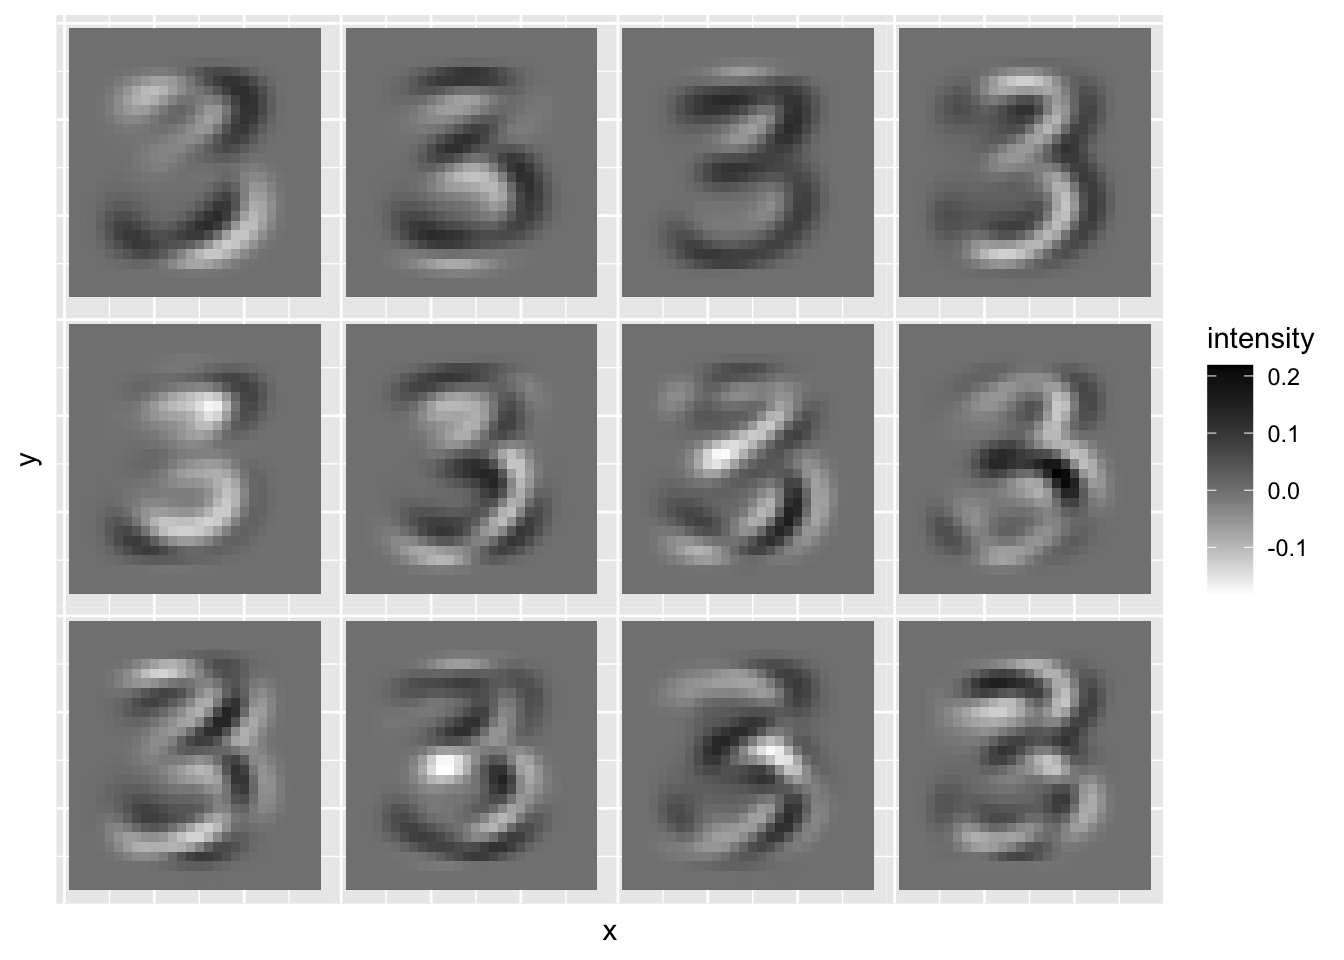
\includegraphics{04-pca_files/figure-latex/unnamed-chunk-33-1.pdf}

We can see there is quite a bit of variation between them.
Now lets look at \(\bar{\boldsymbol x}\), the average 3.

\begin{Shaded}
\begin{Highlighting}[]
\NormalTok{xbar=}\KeywordTok{colMeans}\NormalTok{(mnist3)}
\KeywordTok{plot.mnist}\NormalTok{(xbar)}
\end{Highlighting}
\end{Shaded}

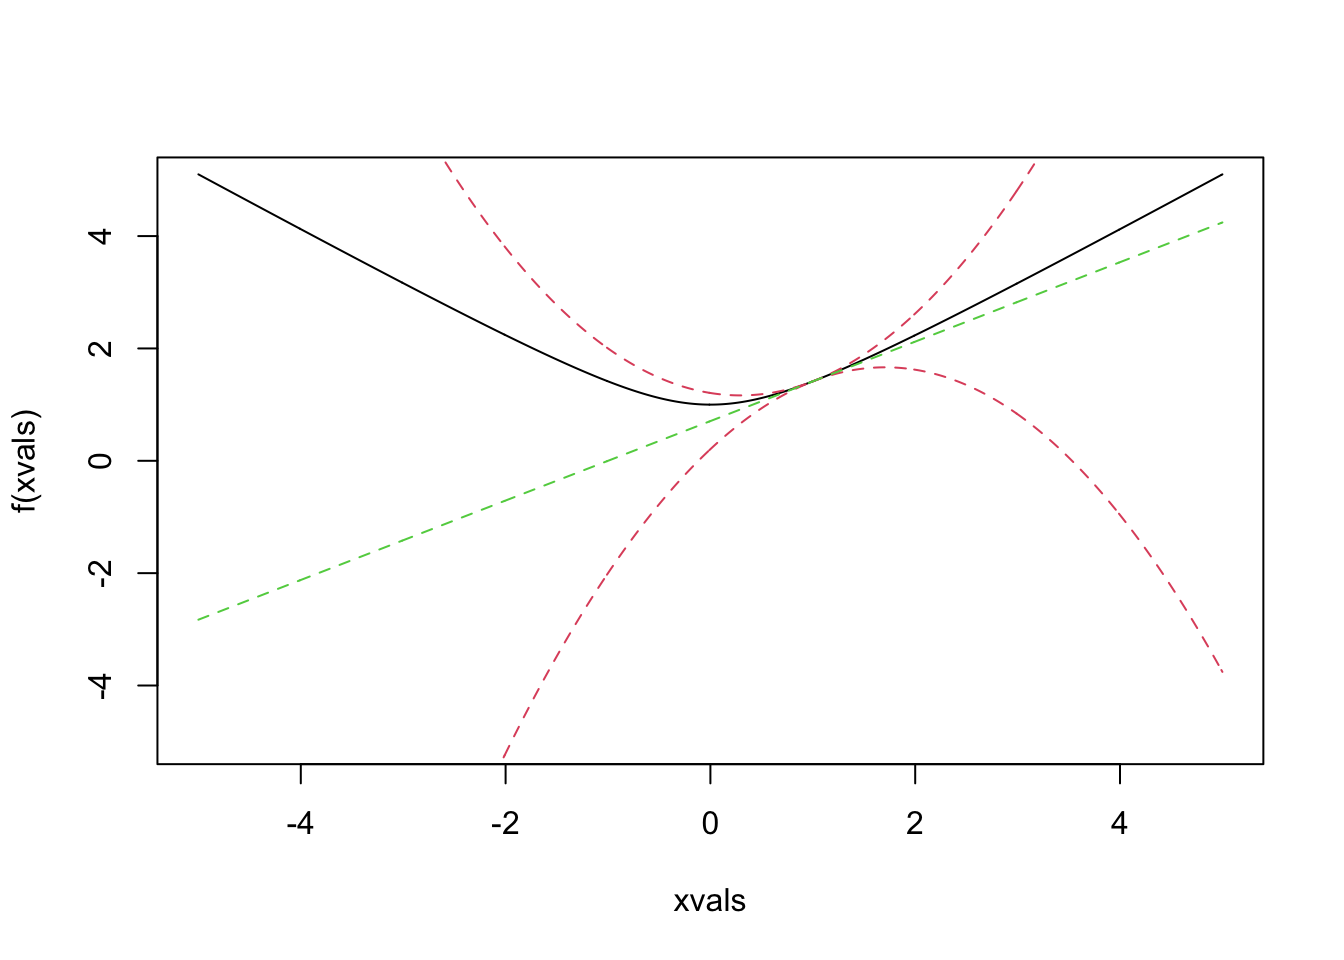
\includegraphics{04-pca_files/figure-latex/unnamed-chunk-34-1.pdf}

We can use the \texttt{prcomp} command to find the principal components. Note that we can't use the \texttt{scale=TRUE} option as some of the columns are all 0, and so R throws an error as it cannot rescale these to have variance 1. Let's plot the first few principal components/eigenvectors/loading vectors.

\begin{Shaded}
\begin{Highlighting}[]
\NormalTok{mnist3.pca <-}\StringTok{ }\KeywordTok{prcomp}\NormalTok{(mnist3)}
\KeywordTok{plot.mnist}\NormalTok{(mnist3.pca}\OperatorTok{$}\NormalTok{rotation[,}\DecValTok{1}\OperatorTok{:}\DecValTok{12}\NormalTok{]) }
\end{Highlighting}
\end{Shaded}

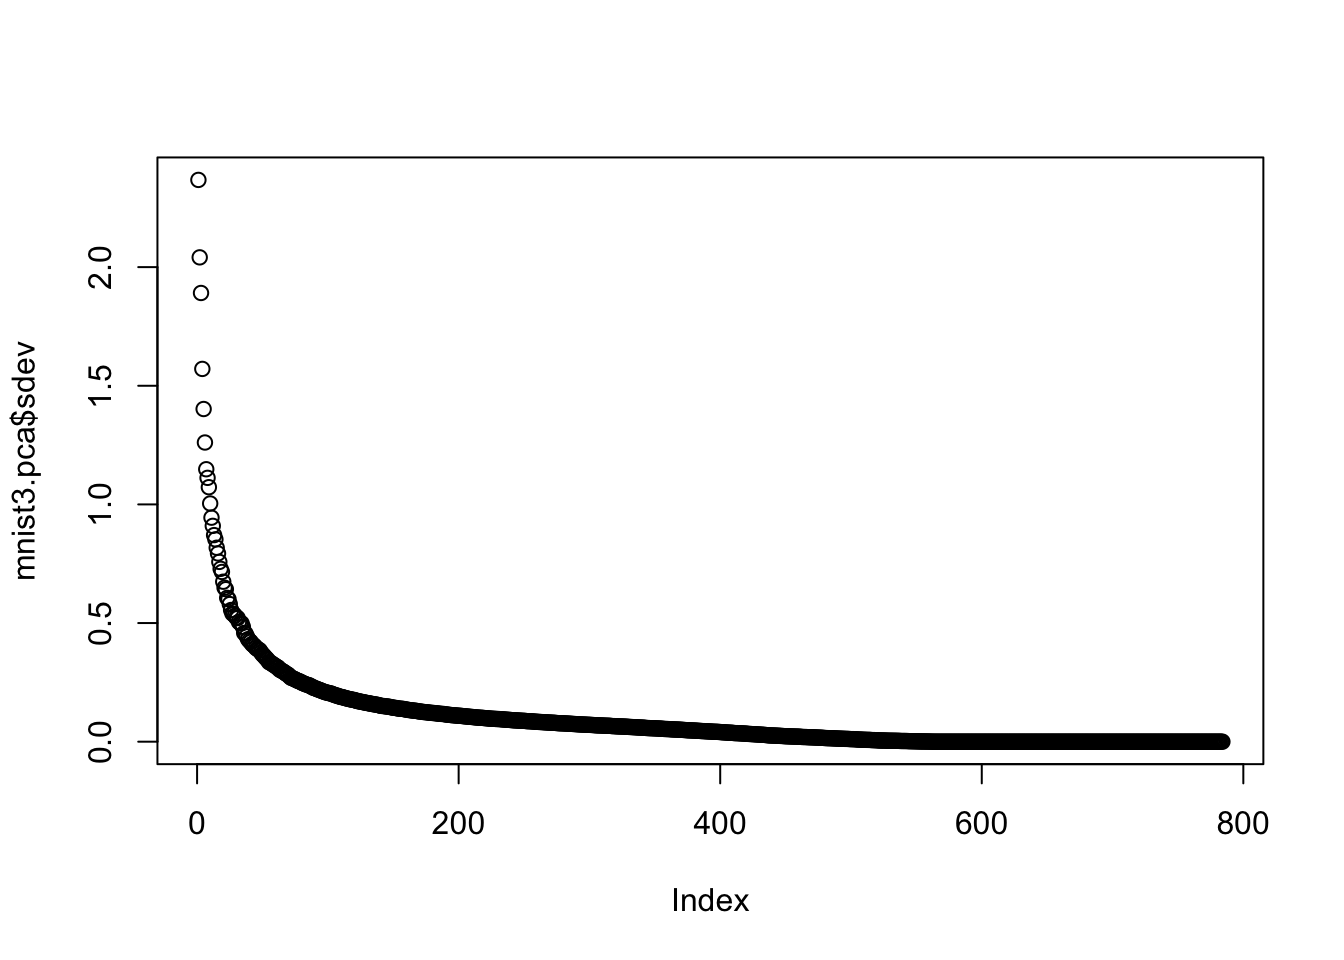
\includegraphics{04-pca_files/figure-latex/unnamed-chunk-35-1.pdf}

These show the main mode of variability in the 3s. Focusing on the first PC, we can see that this is a form of rotation and causes the 3 to slant either forward or backward. If we wanted a rank-2 approximation to the data we would use
\[f(\boldsymbol y) = \bar{\boldsymbol x} + y_1 \boldsymbol v_1 + y_2 \boldsymbol v_2\]

Let's try reconstructing the data with \(r=2\).

\begin{Shaded}
\begin{Highlighting}[]
\NormalTok{r=}\DecValTok{2}
\NormalTok{recon =}\StringTok{  }\NormalTok{mnist3.pca}\OperatorTok{$}\NormalTok{x[,}\DecValTok{1}\OperatorTok{:}\NormalTok{r] }\OperatorTok\StringTok{ }\KeywordTok{t}\NormalTok{(mnist3.pca}\OperatorTok{$}\NormalTok{rotation[,}\DecValTok{1}\OperatorTok{:}\NormalTok{r])}
\KeywordTok{plot.mnist2}\NormalTok{(}\KeywordTok{matrix}\NormalTok{(}\KeywordTok{rep}\NormalTok{(xbar,}\DecValTok{12}\NormalTok{), }\DataTypeTok{byrow=}\NormalTok{T, }\DataTypeTok{nr=}\DecValTok{12}\NormalTok{)}\OperatorTok{+}\NormalTok{recon[}\DecValTok{1}\OperatorTok{:}\DecValTok{12}\NormalTok{,])}
\end{Highlighting}
\end{Shaded}

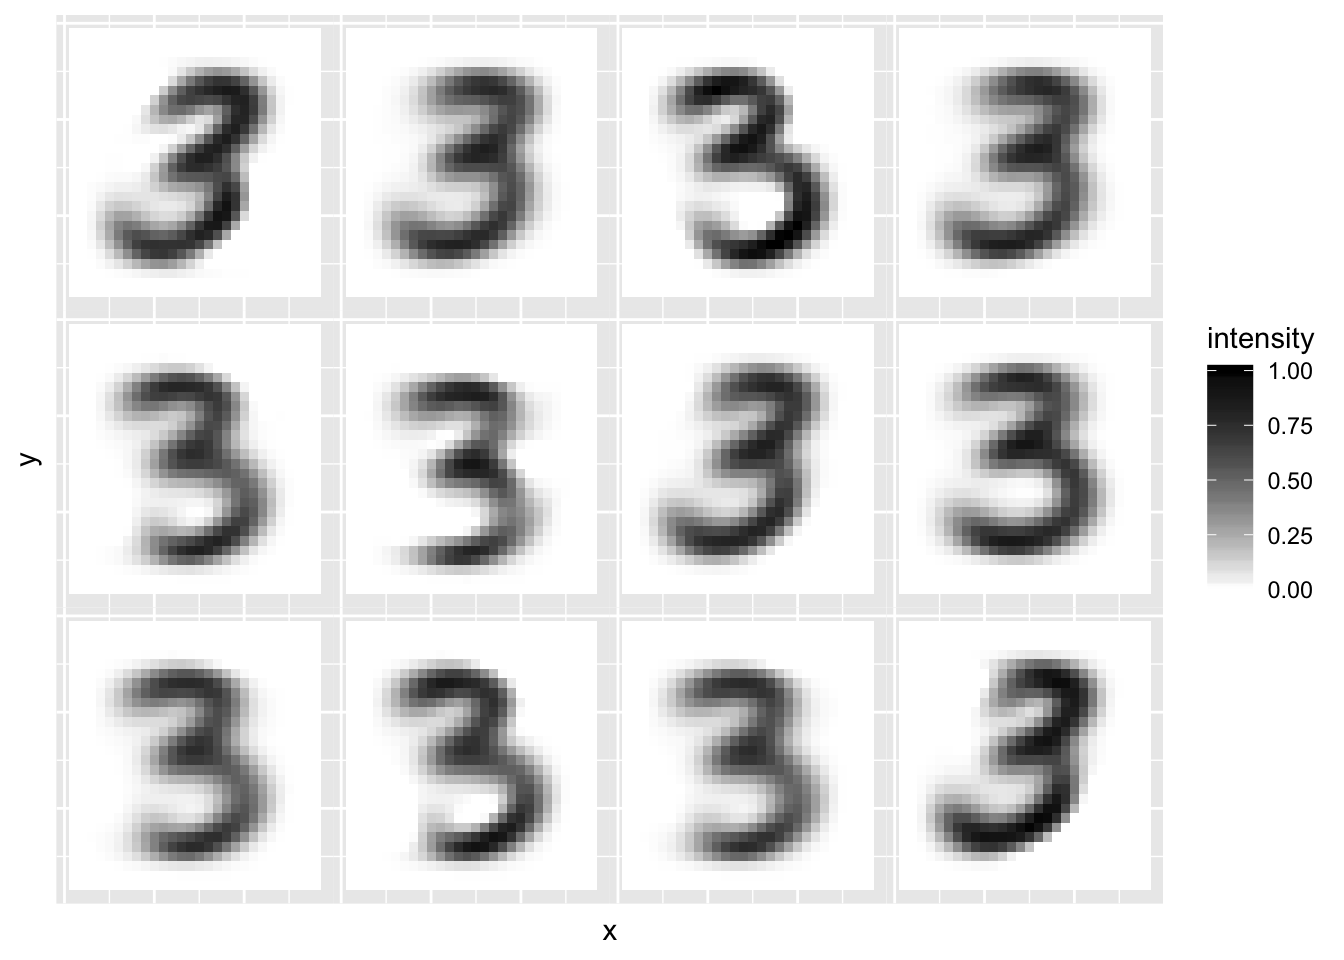
\includegraphics{04-pca_files/figure-latex/unnamed-chunk-36-1.pdf}

We can see that all of these 3s still look a lot like the average 3, but that they vary in their slant, and the heaviness of the line.

The scree plot shows a sharp decrease in the eigenvalues until about the 100th component, at which point they level off.

\begin{Shaded}
\begin{Highlighting}[]
\KeywordTok{plot}\NormalTok{(mnist3.pca}\OperatorTok{$}\NormalTok{sdev) }\CommentTok{# scree plot}
\end{Highlighting}
\end{Shaded}

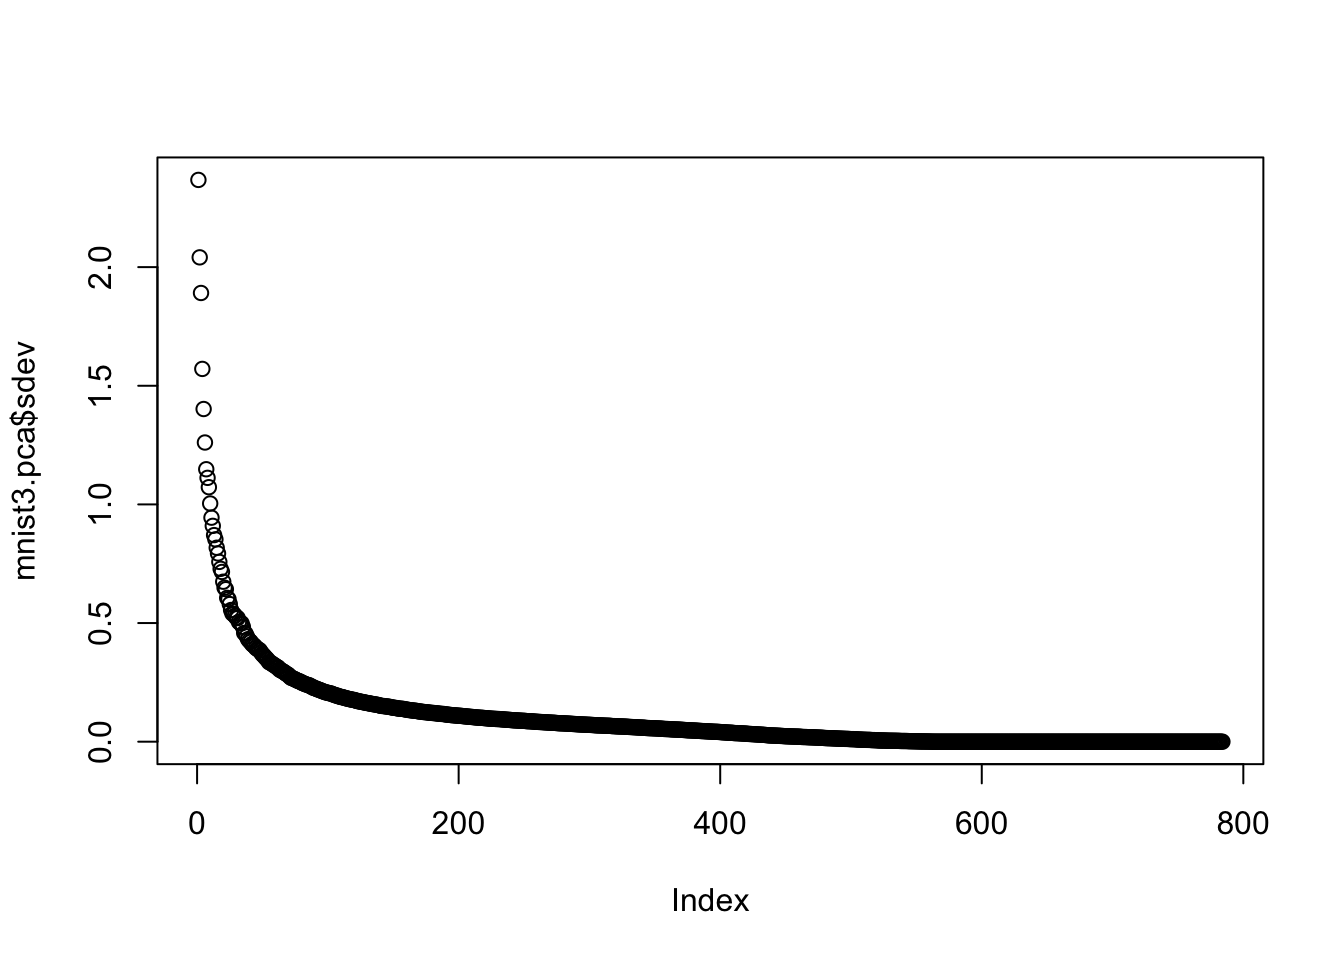
\includegraphics{04-pca_files/figure-latex/unnamed-chunk-37-1.pdf}

It can also be useful to plot the cumulative sum of the total proportion of variance explained by a given number of principal components. I've drawn on horizontal lines at 90\% and 95\% of variance explained, to help identify when we cross these thresholds.
We need 80 components to explain 90\% of the variance, and 138 components to explain 95\% of the variance.

\begin{Shaded}
\begin{Highlighting}[]
\NormalTok{cumvar =}\StringTok{ }\DecValTok{100}\OperatorTok{*}\KeywordTok{cumsum}\NormalTok{(mnist3.pca}\OperatorTok{$}\NormalTok{sdev}\OperatorTok{^}\DecValTok{2}\NormalTok{) }\OperatorTok{/}\StringTok{ }\KeywordTok{sum}\NormalTok{(mnist3.pca}\OperatorTok{$}\NormalTok{sdev}\OperatorTok{^}\DecValTok{2}\NormalTok{)}
\KeywordTok{plot}\NormalTok{(cumvar, }\DataTypeTok{ylab=}\StringTok{"Cumulative proportion of variance explained"}\NormalTok{, }\DataTypeTok{xlab=}\StringTok{"Number of PCs used"}\NormalTok{, }\DataTypeTok{ylim=}\KeywordTok{c}\NormalTok{(}\DecValTok{0}\NormalTok{,}\DecValTok{100}\NormalTok{))}
\KeywordTok{abline}\NormalTok{(}\DataTypeTok{h=}\DecValTok{90}\NormalTok{, }\DataTypeTok{lty=}\DecValTok{2}\NormalTok{)}
\KeywordTok{abline}\NormalTok{(}\DataTypeTok{v=}\KeywordTok{min}\NormalTok{(}\KeywordTok{which}\NormalTok{(cumvar}\OperatorTok{>}\DecValTok{90}\NormalTok{)), }\DataTypeTok{lty=}\DecValTok{2}\NormalTok{)}
\KeywordTok{abline}\NormalTok{(}\DataTypeTok{h=}\DecValTok{95}\NormalTok{, }\DataTypeTok{lty=}\DecValTok{2}\NormalTok{)}
\KeywordTok{abline}\NormalTok{(}\DataTypeTok{v=}\KeywordTok{min}\NormalTok{(}\KeywordTok{which}\NormalTok{(cumvar}\OperatorTok{>}\DecValTok{95}\NormalTok{)), }\DataTypeTok{lty=}\DecValTok{2}\NormalTok{)}
\end{Highlighting}
\end{Shaded}

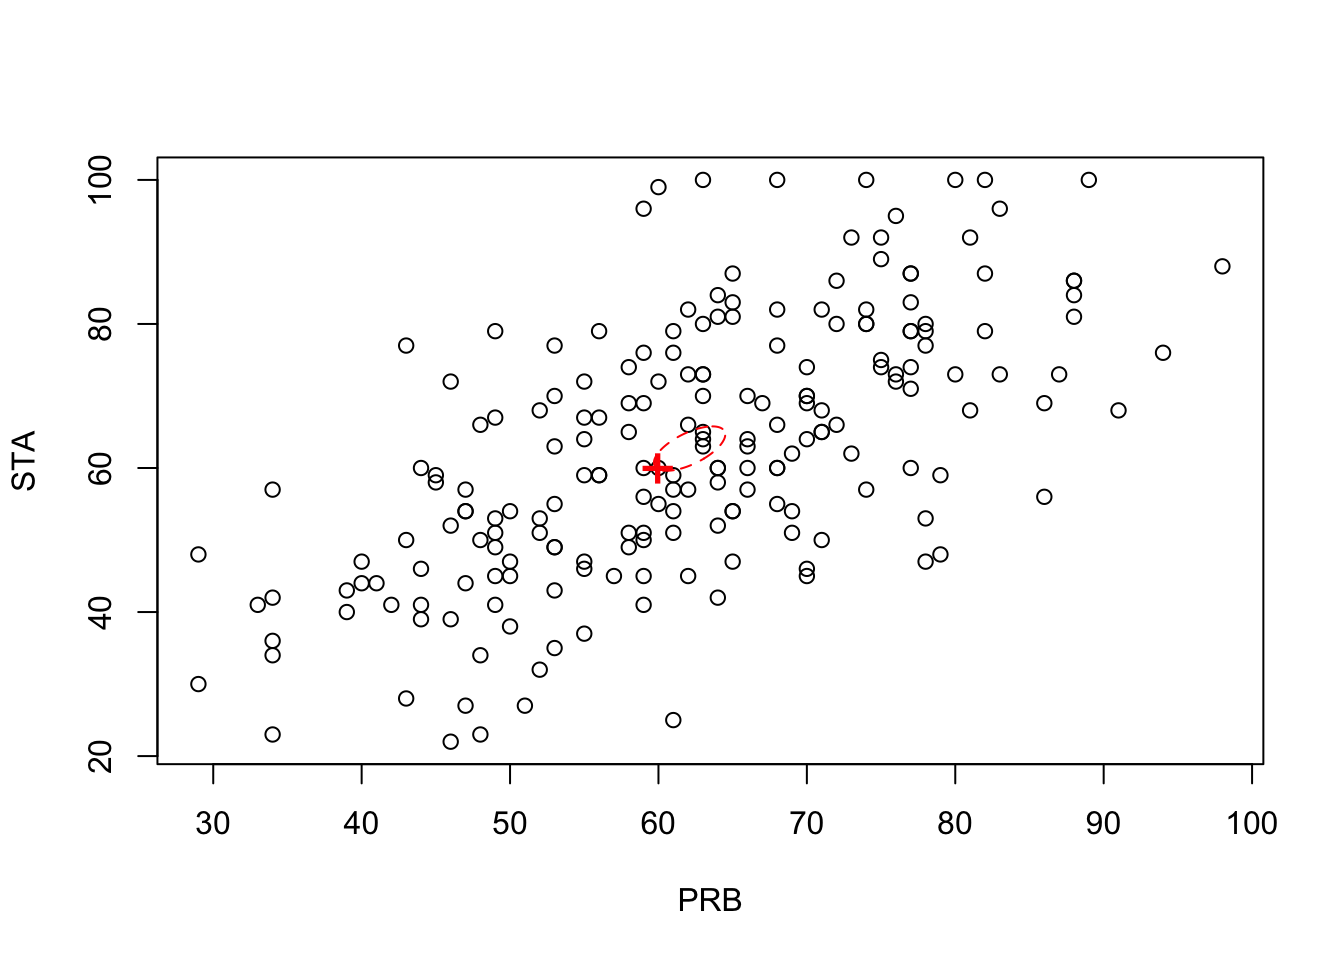
\includegraphics{04-pca_files/figure-latex/unnamed-chunk-39-1.pdf}

Let's now look at the reconstruction using \(r=10, \;50, \;100\) and \(500\) components to see how the accuracy changes.

\begin{Shaded}
\begin{Highlighting}[]
\NormalTok{r=}\DecValTok{10}
\NormalTok{recon =}\StringTok{  }\NormalTok{mnist3.pca}\OperatorTok{$}\NormalTok{x[,}\DecValTok{1}\OperatorTok{:}\NormalTok{r] }\OperatorTok\StringTok{ }\KeywordTok{t}\NormalTok{(mnist3.pca}\OperatorTok{$}\NormalTok{rotation[,}\DecValTok{1}\OperatorTok{:}\NormalTok{r])}
\KeywordTok{plot.mnist2}\NormalTok{(}\KeywordTok{matrix}\NormalTok{(}\KeywordTok{rep}\NormalTok{(xbar,}\DecValTok{12}\NormalTok{), }\DataTypeTok{byrow=}\NormalTok{T, }\DataTypeTok{nr=}\DecValTok{12}\NormalTok{)}\OperatorTok{+}\NormalTok{recon[}\DecValTok{1}\OperatorTok{:}\DecValTok{12}\NormalTok{,])}
\end{Highlighting}
\end{Shaded}

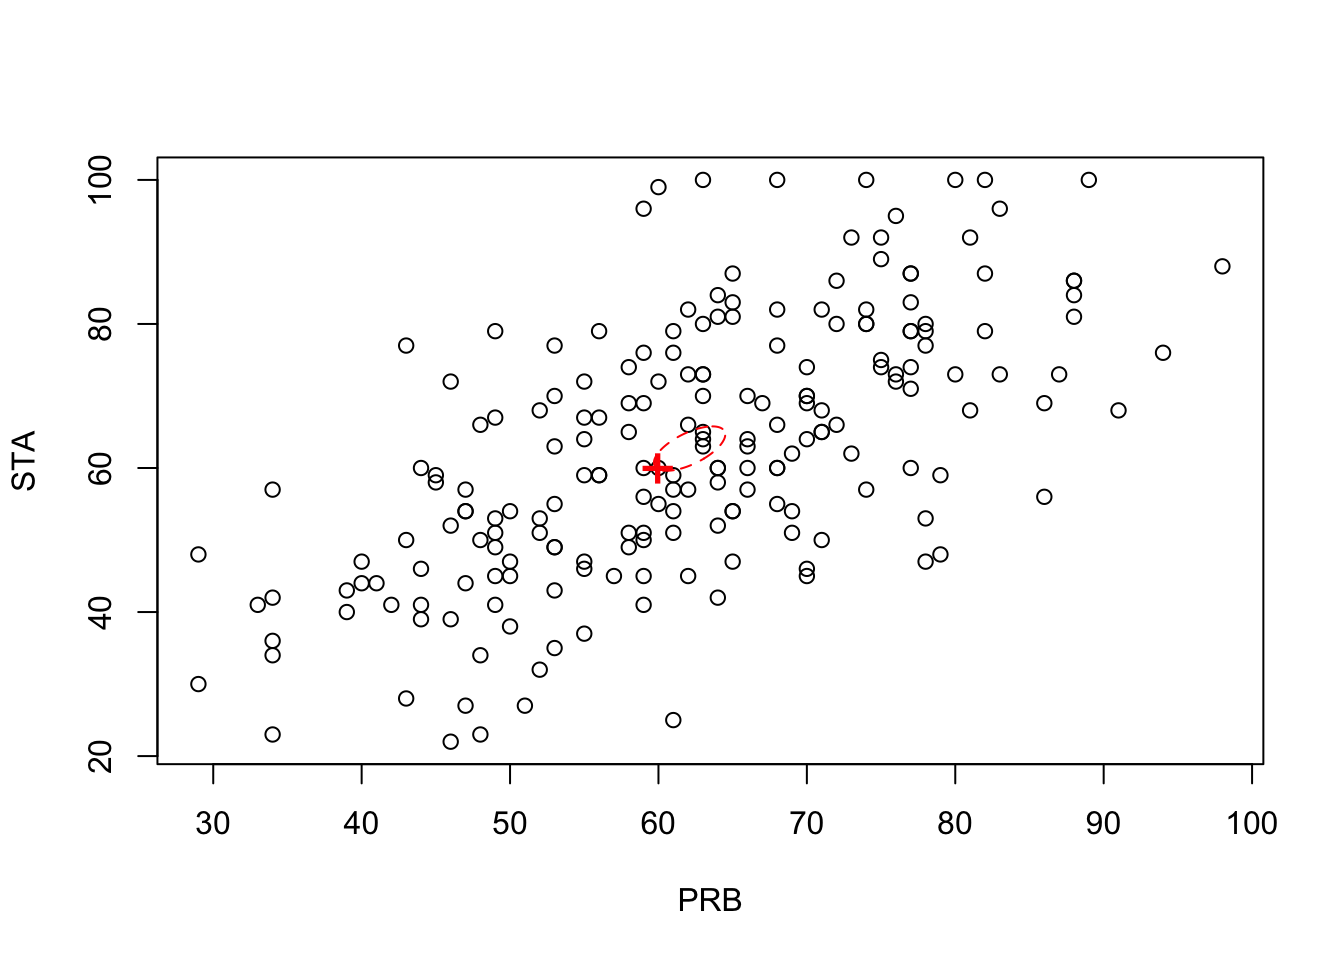
\includegraphics{04-pca_files/figure-latex/unnamed-chunk-40-1.pdf}

\begin{Shaded}
\begin{Highlighting}[]
\NormalTok{r=}\DecValTok{50}
\NormalTok{recon =}\StringTok{  }\NormalTok{mnist3.pca}\OperatorTok{$}\NormalTok{x[,}\DecValTok{1}\OperatorTok{:}\NormalTok{r] }\OperatorTok\StringTok{ }\KeywordTok{t}\NormalTok{(mnist3.pca}\OperatorTok{$}\NormalTok{rotation[,}\DecValTok{1}\OperatorTok{:}\NormalTok{r])}
\KeywordTok{plot.mnist2}\NormalTok{(}\KeywordTok{matrix}\NormalTok{(}\KeywordTok{rep}\NormalTok{(xbar,}\DecValTok{12}\NormalTok{), }\DataTypeTok{byrow=}\NormalTok{T, }\DataTypeTok{nr=}\DecValTok{12}\NormalTok{)}\OperatorTok{+}\NormalTok{recon[}\DecValTok{1}\OperatorTok{:}\DecValTok{12}\NormalTok{,])}
\end{Highlighting}
\end{Shaded}

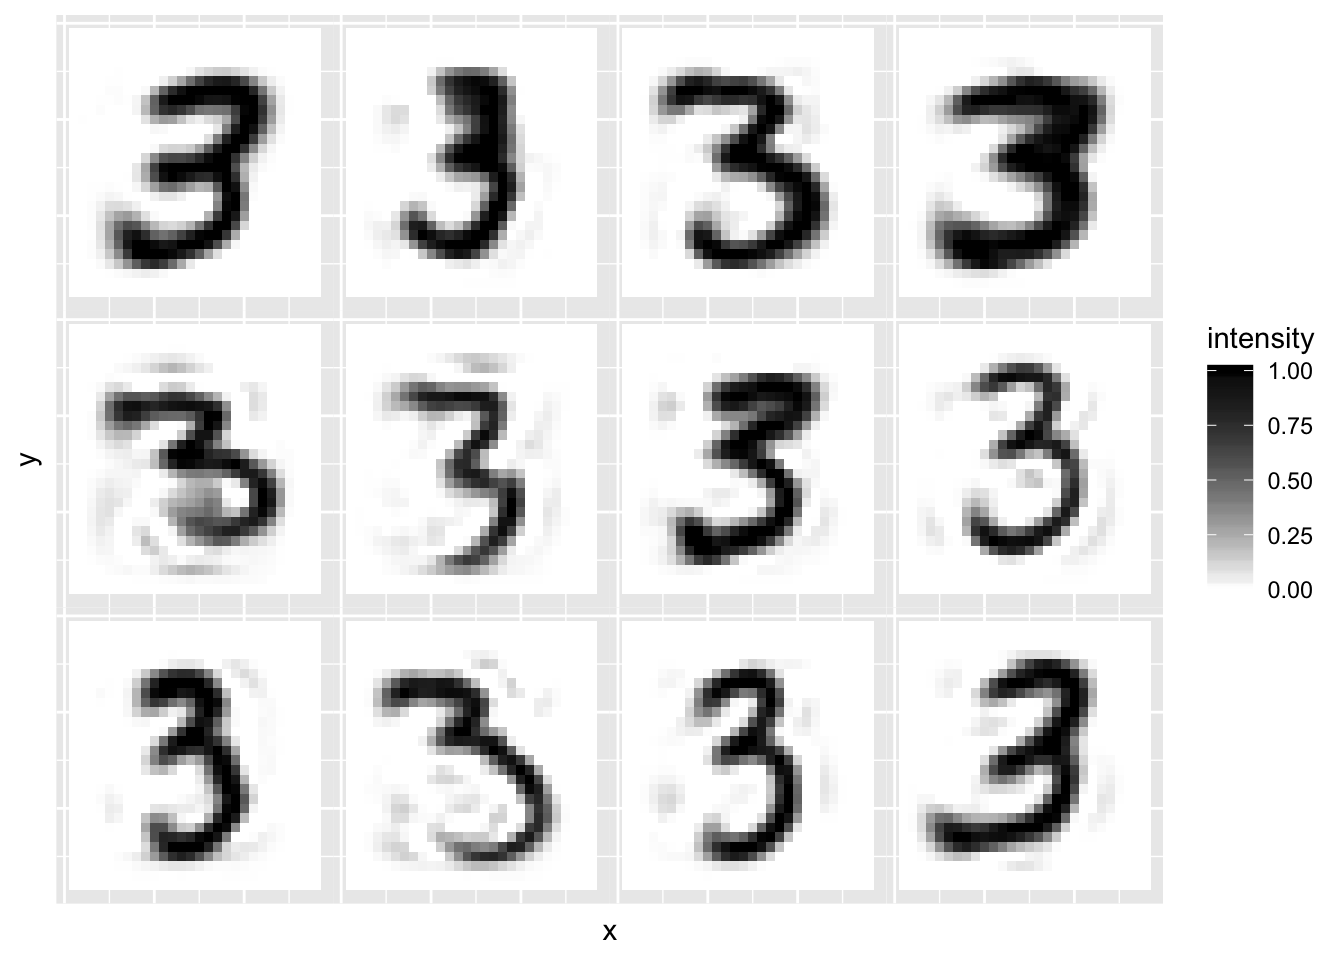
\includegraphics{04-pca_files/figure-latex/unnamed-chunk-41-1.pdf}

\begin{Shaded}
\begin{Highlighting}[]
\NormalTok{r=}\DecValTok{100}
\NormalTok{recon =}\StringTok{  }\NormalTok{mnist3.pca}\OperatorTok{$}\NormalTok{x[,}\DecValTok{1}\OperatorTok{:}\NormalTok{r] }\OperatorTok\StringTok{ }\KeywordTok{t}\NormalTok{(mnist3.pca}\OperatorTok{$}\NormalTok{rotation[,}\DecValTok{1}\OperatorTok{:}\NormalTok{r])}
\KeywordTok{plot.mnist2}\NormalTok{(}\KeywordTok{matrix}\NormalTok{(}\KeywordTok{rep}\NormalTok{(xbar,}\DecValTok{12}\NormalTok{), }\DataTypeTok{byrow=}\NormalTok{T, }\DataTypeTok{nr=}\DecValTok{12}\NormalTok{)}\OperatorTok{+}\NormalTok{recon[}\DecValTok{1}\OperatorTok{:}\DecValTok{12}\NormalTok{,])}
\end{Highlighting}
\end{Shaded}

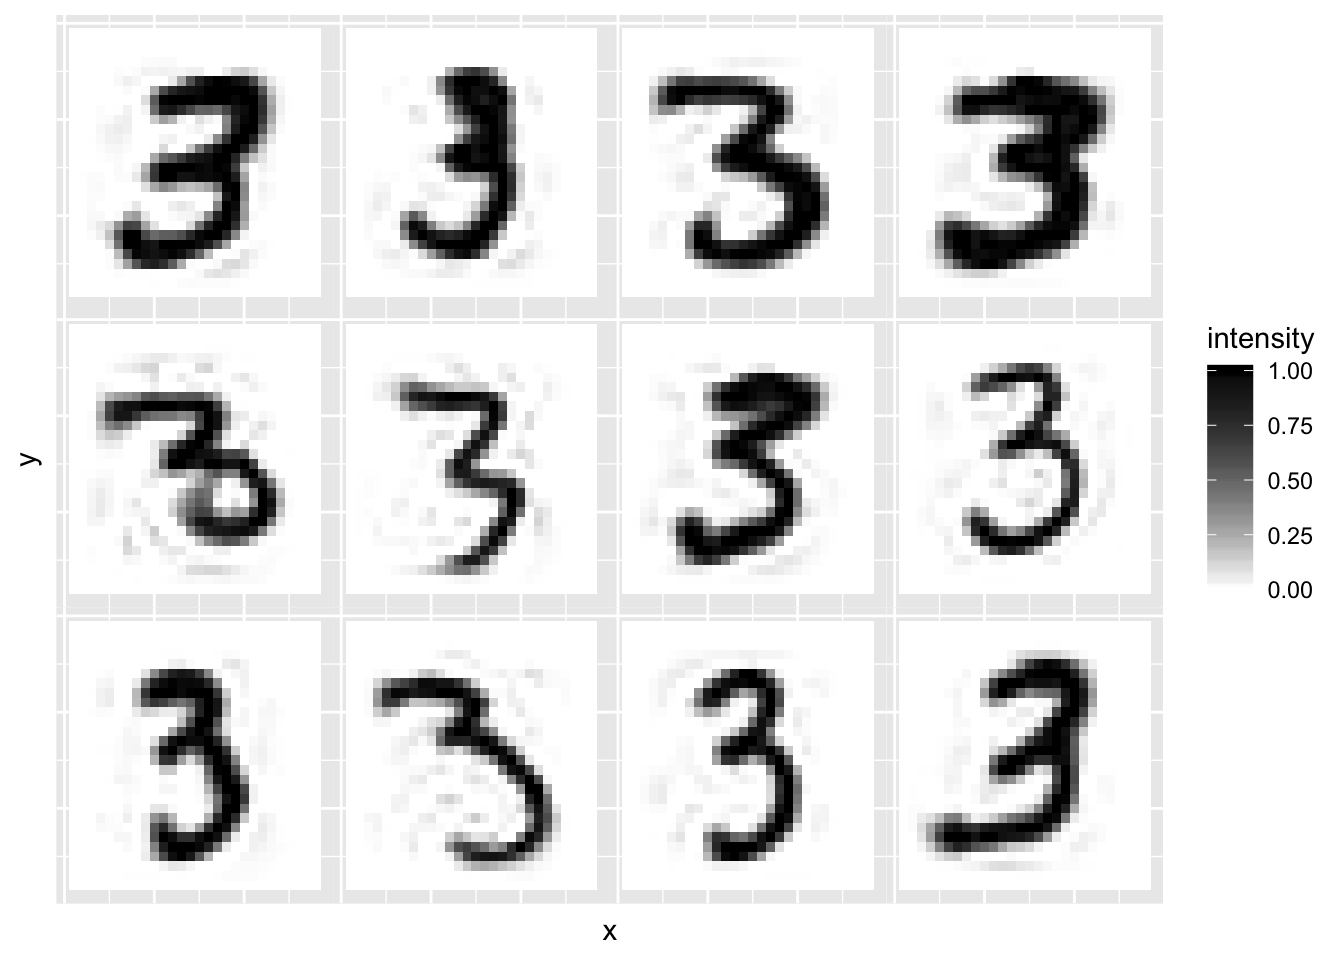
\includegraphics{04-pca_files/figure-latex/unnamed-chunk-42-1.pdf}

\begin{Shaded}
\begin{Highlighting}[]
\NormalTok{r=}\DecValTok{500}
\NormalTok{recon =}\StringTok{  }\NormalTok{mnist3.pca}\OperatorTok{$}\NormalTok{x[,}\DecValTok{1}\OperatorTok{:}\NormalTok{r] }\OperatorTok\StringTok{ }\KeywordTok{t}\NormalTok{(mnist3.pca}\OperatorTok{$}\NormalTok{rotation[,}\DecValTok{1}\OperatorTok{:}\NormalTok{r])}
\KeywordTok{plot.mnist2}\NormalTok{(}\KeywordTok{matrix}\NormalTok{(}\KeywordTok{rep}\NormalTok{(xbar,}\DecValTok{12}\NormalTok{), }\DataTypeTok{byrow=}\NormalTok{T, }\DataTypeTok{nr=}\DecValTok{12}\NormalTok{)}\OperatorTok{+}\NormalTok{recon[}\DecValTok{1}\OperatorTok{:}\DecValTok{12}\NormalTok{,])}
\end{Highlighting}
\end{Shaded}

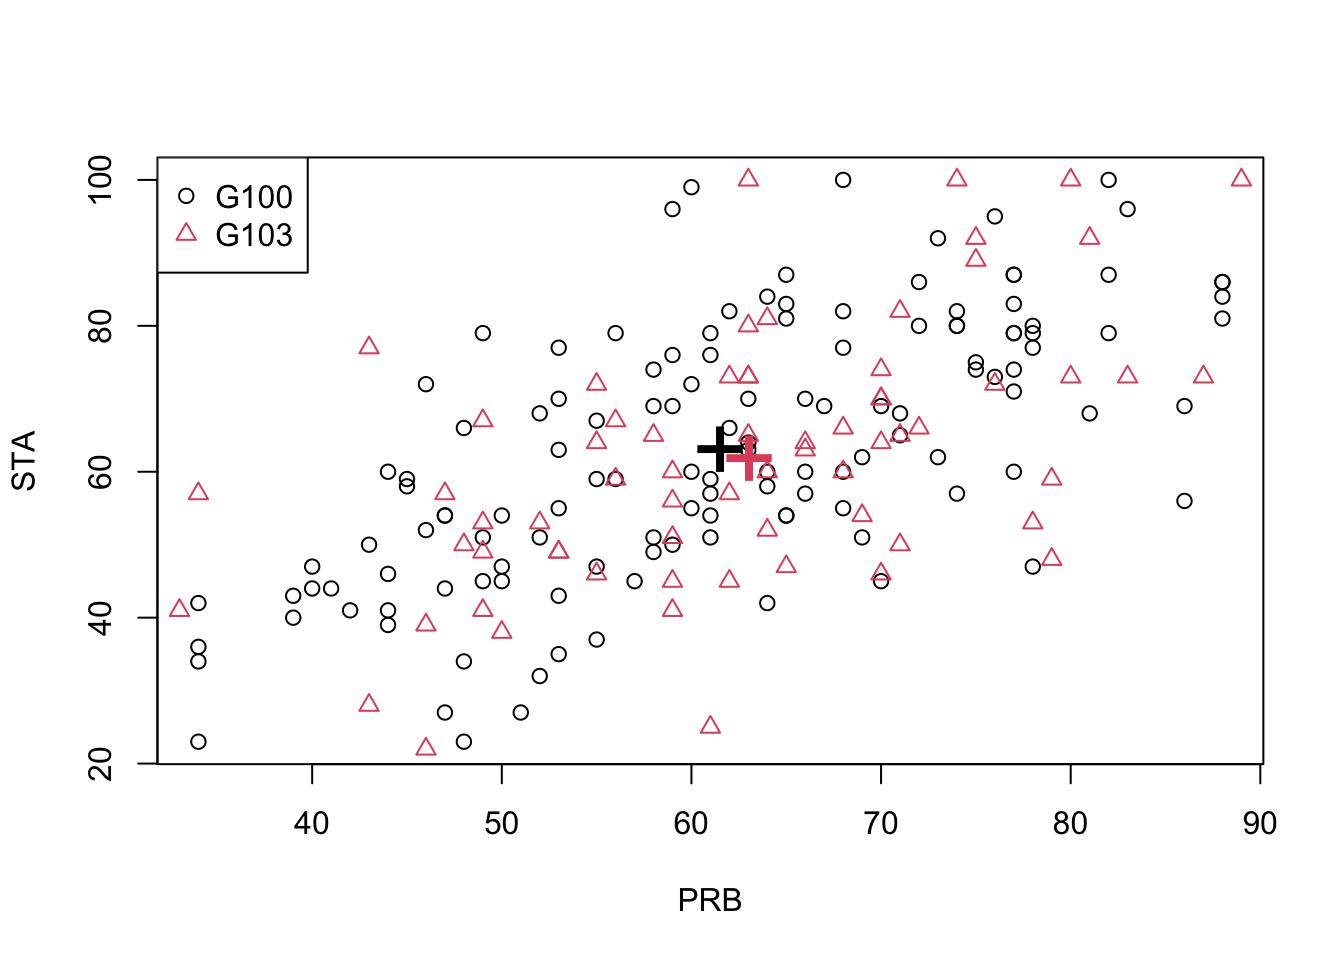
\includegraphics{04-pca_files/figure-latex/unnamed-chunk-43-1.pdf}

We can see that as the number of components increases the reconstructions start to look more like the original 12 images.

We can visualise the range of 3s by looking at a scatter plot of the first two principal components.

\begin{Shaded}
\begin{Highlighting}[]
\KeywordTok{library}\NormalTok{(ggplot2)}
\KeywordTok{qplot}\NormalTok{(mnist3.pca}\OperatorTok{$}\NormalTok{x[,}\DecValTok{1}\NormalTok{], mnist3.pca}\OperatorTok{$}\NormalTok{x[,}\DecValTok{2}\NormalTok{])}
\end{Highlighting}
\end{Shaded}

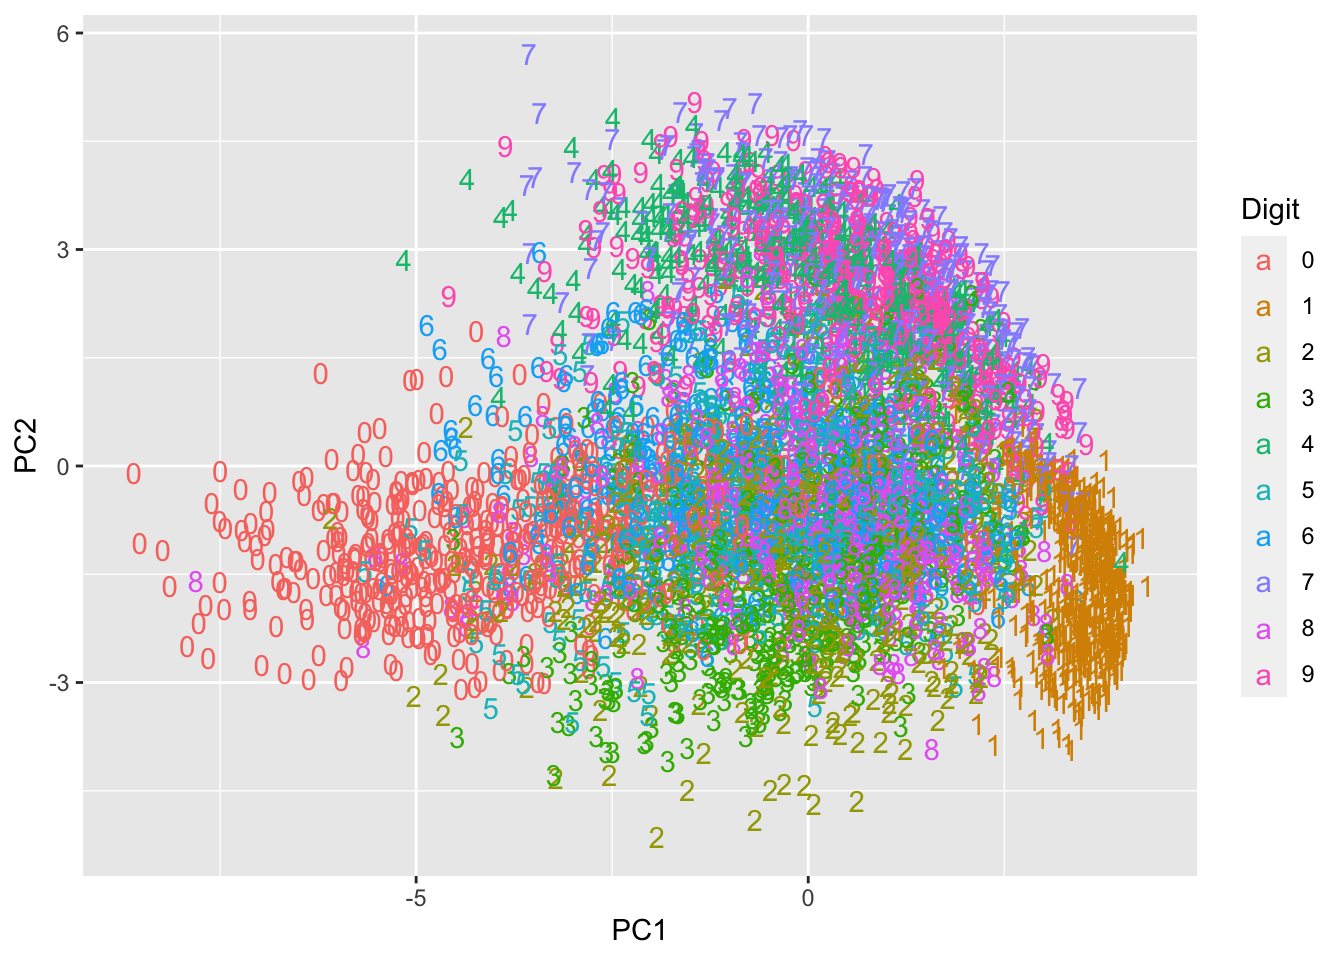
\includegraphics{04-pca_files/figure-latex/unnamed-chunk-44-1.pdf}

We can then finding images that differ according to these two PC scores. The first plot below is the 3 with the smallest PC1 score, and the second has the largest PC1 score. The third plot has the smallest PC2 score, and the fourth plot the largest PC2 score.
These four different 3s differ in more than just the first two principal components, but you can see the effect of the PC1 score is to slant the image forward or backward, whereas PC2 changes the thickness of the line.

\begin{Shaded}
\begin{Highlighting}[]
\NormalTok{image_list <-}\StringTok{ }\KeywordTok{c}\NormalTok{(}\KeywordTok{which.min}\NormalTok{(mnist3.pca}\OperatorTok{$}\NormalTok{x[,}\DecValTok{1}\NormalTok{]), }\KeywordTok{which.max}\NormalTok{(mnist3.pca}\OperatorTok{$}\NormalTok{x[,}\DecValTok{1}\NormalTok{]), }\KeywordTok{which.min}\NormalTok{(mnist3.pca}\OperatorTok{$}\NormalTok{x[,}\DecValTok{2}\NormalTok{]), }\KeywordTok{which.max}\NormalTok{(mnist3.pca}\OperatorTok{$}\NormalTok{x[,}\DecValTok{2}\NormalTok{]))}
\KeywordTok{plot.mnist}\NormalTok{(mnist3[image_list,]) }\CommentTok{# plot the first 12 images}
\end{Highlighting}
\end{Shaded}

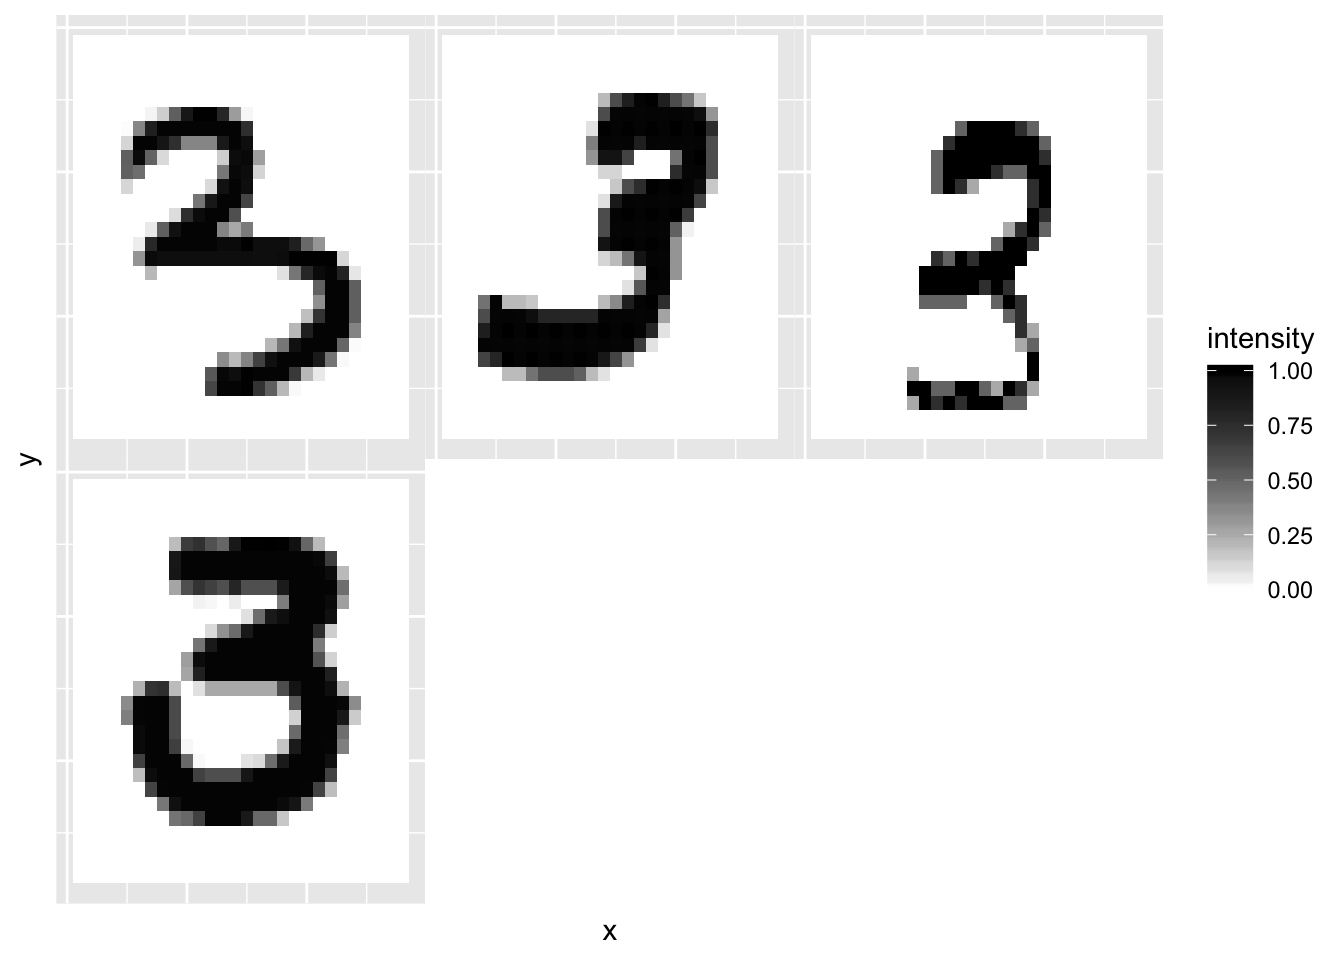
\includegraphics{04-pca_files/figure-latex/unnamed-chunk-45-1.pdf}

Finally, let's do PCA on a selection of the 60,000 images (not just the 3s). You can compute the SVD (which is what \texttt{prcomp} uses to do PCA) on a \(60,000 \times 784\) matrix, but it takes a long time on most computers, so here I've just computed the first two components on a random selection of 5,000 images using the option \texttt{rank=2} which significantly speeds up the computation time.

\begin{Shaded}
\begin{Highlighting}[]
\CommentTok{# Note this is slow to compute!}
\NormalTok{image_index <-}\StringTok{ }\KeywordTok{sample}\NormalTok{(}\DecValTok{1}\OperatorTok{:}\DecValTok{60000}\NormalTok{, }\DataTypeTok{size=}\DecValTok{5000}\NormalTok{) }\CommentTok{# select a random sample of images}
\NormalTok{mnist.pca <-}\StringTok{ }\KeywordTok{prcomp}\NormalTok{(mnist}\OperatorTok{$}\NormalTok{train}\OperatorTok{$}\NormalTok{x[image_index,], }\DataTypeTok{rank=}\DecValTok{2}\NormalTok{)}
\NormalTok{Digit =}\StringTok{ }\KeywordTok{as.factor}\NormalTok{(mnist}\OperatorTok{$}\NormalTok{train}\OperatorTok{$}\NormalTok{y[image_index])}
\KeywordTok{ggplot}\NormalTok{(}\KeywordTok{as.data.frame}\NormalTok{(mnist.pca}\OperatorTok{$}\NormalTok{x), }\KeywordTok{aes}\NormalTok{(}\DataTypeTok{x=}\NormalTok{PC1, }\DataTypeTok{y=}\NormalTok{PC2, }\DataTypeTok{colour=}\NormalTok{Digit, }\DataTypeTok{label=}\NormalTok{Digit)) }\OperatorTok{+}\KeywordTok{geom_text}\NormalTok{(}\KeywordTok{aes}\NormalTok{(}\DataTypeTok{label=}\NormalTok{Digit))}
\end{Highlighting}
\end{Shaded}

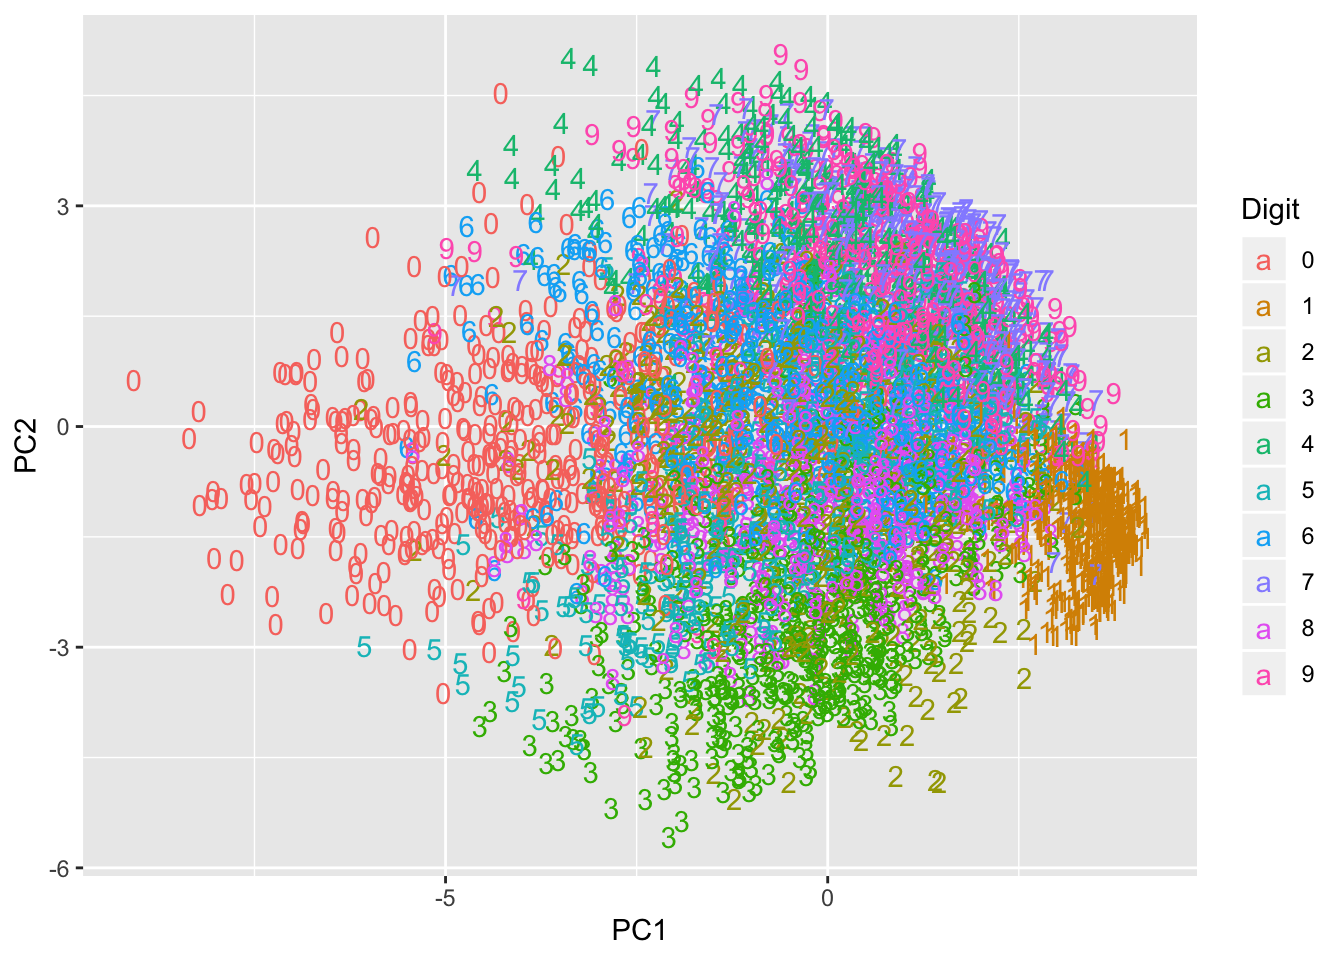
\includegraphics{04-pca_files/figure-latex/unnamed-chunk-46-1.pdf}

We can see from this scatter plot that the first two principal components do a surprisingly good job of separating and clustering the digits.

\hypertarget{computer-tasks-1}{%
\section{Computer tasks}\label{computer-tasks-1}}

\begin{enumerate}
\def\labelenumi{\arabic{enumi}.}
\item
  Using the \texttt{iris} dataset, familiarize yourself with the \texttt{prcomp} command and its output.

  Now, instead of using \texttt{prcomp} we will do the analysis ourselves using the \texttt{eigen} command.
\end{enumerate}

\begin{itemize}
\tightlist
\item
  Start by computing the sample mean and sample variance of the dataset (use \(n-1\) as the denominator when you compute the sample variance to get the same answer as provided by \texttt{prcomp}).
\item
  Now compute the eigenvalues and eigenvectors of the covariance matrix using \texttt{eigen}. Check that these agree with those computed by \texttt{prcomp} (noting that \texttt{prcomp} returns the standard deviation which is the square root of the eigenvalues).
\item
  Now compute the principal component scores by multiplying \(\boldsymbol X\) by the matrix of eigenvectors \(\boldsymbol V\). Check your answer agrees with the scores provided by \texttt{prcomp}.
\end{itemize}

Now we will do the same thing again, but using the \texttt{svd} command.

\begin{itemize}
\tightlist
\item
  Compute the column centred data matrix \(\frac{1}{\sqrt{n-1}}\boldsymbol H\boldsymbol X\)
\item
  Compute the SVD of this matrix. Check the singular values match the square root of the eigenvalues computed previously.
\item
  Compute the SVD scores by doing both \(\boldsymbol X\boldsymbol V\) and \(\boldsymbol U\boldsymbol \Sigma\).
\end{itemize}

\begin{enumerate}
\def\labelenumi{\arabic{enumi}.}
\setcounter{enumi}{1}
\tightlist
\item
  We first look at the crabs data, which is a dataset in the MASS library. First, we obtain the data.
  Then we focus on 5 continuous variables, all measured in mm: FL = frontal lobe size; RW = rear width; CL = carapace length;
  CW = carapace width; and BD = body depth. The sample size is \(200\).
\end{enumerate}

\begin{Shaded}
\begin{Highlighting}[]
\KeywordTok{library}\NormalTok{(MASS)}
\NormalTok{?crabs           }\CommentTok{# read the help page to find out about the dataset}
\NormalTok{X=crabs[}\DecValTok{4}\OperatorTok{:}\DecValTok{8}\NormalTok{]     }\CommentTok{# construct data matrix X with columns FL, RW, CL, CW, BD}
\end{Highlighting}
\end{Shaded}

\begin{verbatim}
Carry out PCA on the data in $X$, including obtaining a scree plot and plotting the PC scores.
\end{verbatim}

\begin{Shaded}
\begin{Highlighting}[]
\NormalTok{pca <-}\StringTok{ }\KeywordTok{prcomp}\NormalTok{(X, }\DataTypeTok{scale=}\OtherTok{FALSE}\NormalTok{)   }\CommentTok{#carry out PCA on S  }
\NormalTok{pca}
\NormalTok{lambda <-}\StringTok{ }\NormalTok{pca}\OperatorTok{$}\NormalTok{sdev}\OperatorTok{**}\DecValTok{2}    \CommentTok{#eigenvalues of S}
\KeywordTok{plot}\NormalTok{( lambda , }\DataTypeTok{ylim=}\KeywordTok{c}\NormalTok{( }\DecValTok{0}\NormalTok{, }\KeywordTok{max}\NormalTok{(lambda) )}
\KeywordTok{lines}\NormalTok{(lambda)}
\end{Highlighting}
\end{Shaded}

Some questions:

\begin{itemize}
\item
  Do you have any suggestions for an interpretation for the 1st PC?
\item
  Are you able to come up with an interpretation for the 2nd PC?
\item
  Do you think an analysis based on the sample covariance matrix \({\bf S}\) or the
  correlation matrix \({\bf R}\) is preferable with this dataset? Note that you can use \{\tt scale=TRUE\} in \{\tt prcomp\}
  to carry out PCA on \({\bf R}\). Does it make much difference which is used?
\end{itemize}

\hypertarget{exercises-1}{%
\section{Exercises}\label{exercises-1}}

\begin{enumerate}
\def\labelenumi{\arabic{enumi}.}
\tightlist
\item
  Consider the following data in \(\mathbb{R}^2\)
\end{enumerate}

\[\boldsymbol x_1 =\begin{pmatrix}1\\-1\end{pmatrix},\; \boldsymbol x_2 =\begin{pmatrix}-1\\1\end{pmatrix},
\;\boldsymbol x_3 =\begin{pmatrix}2\\2\end{pmatrix},\;\boldsymbol x_3 =\begin{pmatrix}-2\\-2\end{pmatrix}\]

\begin{itemize}
\item
  What is the orthogonal projection of these points onto \[\boldsymbol u_1 = \begin{pmatrix}1\\0\end{pmatrix}\] and onto \[\boldsymbol u_2 =\frac{1}{\sqrt{5}}\begin{pmatrix}1\\2\end{pmatrix}?\]
\item
  Compute the sample variance matrix of the three data points, and compute its spectral decomposition.
\item
  What vector \(\boldsymbol u\) would maximize the variance of these projection?
\item
  What vector \(\boldsymbol u\) would minimize
  \[\sum_{i=1}^4 ||\boldsymbol x_i -\boldsymbol u\boldsymbol u^\top \boldsymbol x_i||^2_2?\]
  This is the sum of squared errors from a rank 1 approximation to the data.
\item
  Plot the data points and convince yourself that your answers make intuitive sense.
\end{itemize}

\begin{enumerate}
\def\labelenumi{\arabic{enumi}.}
\setcounter{enumi}{1}
\tightlist
\item
  Consider a population covariance matrix \(\boldsymbol \Sigma\) of the form
  \[\boldsymbol \Sigma=\gamma \mathbf I_p + \boldsymbol a\boldsymbol a^\top\]
  where \(\gamma>0\) is a scalar, \(\mathbf I_p\) is the \(p \times p\) identity matrix and \(\boldsymbol a\) is a vector of dimension \(p\).

  \begin{itemize}
  \tightlist
  \item
    Show that \(\boldsymbol a\) is an eigenvector of \(\boldsymbol \Sigma\).
  \item
    Show that if \(\boldsymbol b\) is any vector such that \(\boldsymbol a^\top \boldsymbol b=0\), then \(\boldsymbol b\) is also an eigenvector of \(\boldsymbol \Sigma\).
  \item
    Obtain all the eigenvalues of \(\boldsymbol \Sigma\).
  \item
    Determine expressions for the proportion of (population) variability ``explained'' by:
    - the largest (population) principal component of \(\boldsymbol \Sigma\);
    - the \(r\) largest (population) principal components of \(\boldsymbol \Sigma\), where \(1 < r \leq p\).
  \end{itemize}
\item
  A covariance matrix has the following eigenvalues:
\end{enumerate}

\begin{verbatim}
##  [1] 4.22 2.38 1.88 1.11 0.91 0.82 0.58 0.44 0.35 0.19 0.05 0.04 0.04
\end{verbatim}

\begin{verbatim}
- Sketch a scree plot.
- Determine the minimum number of principal components needed to explain 90\% of the total variation.
- Determine the number of principal components whose eigenvalues are above average.
\end{verbatim}

\begin{enumerate}
\def\labelenumi{\arabic{enumi}.}
\setcounter{enumi}{3}
\tightlist
\item
  Measurements are taken on \(p=3\) variables \(x_1\), \(x_2\) and \(x_3\), with sample correlation matrix
  \[
   \boldsymbol R= \begin{pmatrix} 1 & 0.5792 & 0.2414 \\ 0.5792 & 1 & 0.5816 \\ 0.2414 & 0.5816 & 1 \end{pmatrix}.
  \]
  The variable \(z_j\) is the standardised versions of \(x_j\), \(j=1,2,3\), i.e.~each \(z_j\) has sample mean \(0\) and variance \(1\).
  One observation has \(z_1 = z_2 = z_3 = 0\) and a second observation has \(z_1 = z_2 = z_3 =1\). Calculate the three
  principal component scores for
  each of these observations.
\end{enumerate}

\hypertarget{cca}{%
\chapter{Canonical Correlation Analysis}\label{cca}}

Suppose we observe a random sample of \(n\) bivariate observations
\[
\boldsymbol z_1=(x_1,y_1)^\top , \ldots , \boldsymbol z_n=(x_n,y_n)^\top.
\]
If we are interested in exploring possible dependence between the \(x_i\)'s and \(y_i\)'s then among the first things we would do would be to obtain a scatterplot of the \(x_i\)'s against the \(y_i\)'s and calculate the correlation coefficient. Recall that the sample correlation coefficient is defined by
\begin{equation}
r=r[x,y]=\frac{n^{-1}\sum_{i=1}^n (x_i-\bar{x})(y_i-\bar{y})}{\left ( n^{-1}\sum_{i=1}^n (x_i-\bar{x})^2  \right )^{1/2}  \left ( n^{-1}\sum_{i=1}^n (y_i-\bar{y})^2 \right )^{1/2}}
\label{eq:scr}
\end{equation}
where \(\bar{x}=n^{-1}\sum_{i=1}^n x_i\) and \(\bar{y}=n^{-1}\sum_{i=1}^n y_i\) are the sample means. Note that the sample correlation is a \textbf{scale-free measure} of the strength of \textbf{linear dependence} between the \(x_i\)'s and the \(y_i\)'s.

In this chapter we investigate the multivariate analogue of this question. Suppose
\[
\boldsymbol z_i =(\boldsymbol x_i^\top,\boldsymbol y_i^\top)^\top, \qquad i=1,\ldots, n,
\]
is a random sample of vectors. What is a sensible way to assess and describe the strength of the linear dependence between the \(\boldsymbol x_i\) vectors and the \(\boldsymbol y_i\) vectors? That is what this chapter is about. A key role is played by the singular valued decomposition (SVD) introduced in Result 2.13 in Chapter 2.

\begin{example}
\protect\hypertarget{exm:prem}{}{\label{exm:prem} }From time to time we will return to the Premier League example in this chapter. We shall treat \(W\) and \(D\), the number of wins and draws, respectively, as the \(x\)-variables; and \(F\) and \(A\), the number of goals for and against, will be treated as the \(y\)-variables. The number of losses, \(L\), is omitted as it provides no additional information when we know \(W\) and \(D\). A question we shall consider is: how strongly associated are the match outcome variables, \(W\) and \(D\), with the goals for and against variables, \(F\) and \(A\)?
\end{example}

\hypertarget{canonical-correlation-analysis}{%
\section{Canonical Correlation Analysis}\label{canonical-correlation-analysis}}

Assume we are given a random sample of vectors
\[
\boldsymbol z_i=(\boldsymbol x_i^\top , \boldsymbol y_i^\top )^\top: \, i=1,\ldots, n,
\]
where
the \(\boldsymbol x_i\) are \(p \times 1\), the \(\boldsymbol y_i\) are \(q \times 1\) and, consequently, the \(\boldsymbol z_i\) are \((p+q)\times 1\). We are interested in determining the strength of linear association between the \(\boldsymbol x_i\) vectors and the \(\boldsymbol y_i\) vectors.

Write
\[
\bar{\boldsymbol z}=n^{-1}\sum_{i=1}^n \boldsymbol z_i, \qquad \bar{\boldsymbol x}=n^{-1} \sum_{i=1}^n \boldsymbol x_i \qquad \text{and} \qquad \bar{\boldsymbol y}=n^{-1}\sum_{i=1}^n \boldsymbol y_i
\]
for the sample mean vectors of the \(\boldsymbol z_i\), \(\boldsymbol x_i\) and \(\boldsymbol y_i\) respectively.

We formulate this task as an optimisation problem (cf.~PCA). First, we introduce some notation. Let \(\boldsymbol S_{\boldsymbol z\boldsymbol z}\) denote the sample covariance matrix of the \(\boldsymbol z_i\), \(i=1,\ldots, n\). Then \(\boldsymbol S_{\boldsymbol z\boldsymbol z}\) can be written in block matrix form
\[
\boldsymbol S_{\boldsymbol z\boldsymbol z}=\left [\begin{array}{cc}
\boldsymbol S_{\boldsymbol x\boldsymbol x} & \boldsymbol S_{\boldsymbol x\boldsymbol y}\\
\boldsymbol S_{\boldsymbol y\boldsymbol x} & \boldsymbol S_{\boldsymbol y\boldsymbol y} \end{array} \right ],
\]
where \(\boldsymbol S_{\boldsymbol x\boldsymbol x}\) (\(p \times p\)) is the sample covariance matrix of the \(\boldsymbol x_i\), \(\boldsymbol S_{\boldsymbol y\boldsymbol y}\) (\(q \times q\)) is the sample covariance of the \(\boldsymbol y_i\), and the cross-covariance matrices are given by
\[
\stackrel{p \times q}{\boldsymbol S}_{\boldsymbol x\boldsymbol y}=n^{-1} \sum_{i=1}^n (\boldsymbol x_i -\bar{\boldsymbol x})(\boldsymbol y_i-\bar{\boldsymbol y})^\top
\qquad \text{and} \qquad \stackrel{q \times p}{\boldsymbol S}_{\boldsymbol y\boldsymbol x}=\boldsymbol S_{\boldsymbol x\boldsymbol y}^\top.
\]

\textbf{Example \ref{exm:prem} (continued)}. The relevant covariance matrix here is given in \eqref{eq:PLES},
but we need to delete the middle row and middle column because this relates to the variable \(L\), the number of losses,
which we are omitting. So we are left with
\begin{equation}
\boldsymbol S_{\boldsymbol x\boldsymbol x}=\begin{pmatrix} 39.4 & -8.3\\ -8.3 & 8.1   \end{pmatrix} , \qquad
\boldsymbol S_{\boldsymbol y\boldsymbol y}=\begin{pmatrix} 392.2 & -208.7\\ -208.7 & 230.9   \end{pmatrix}
\label{eq:bSxy1}
\end{equation}
and
\begin{equation}
\boldsymbol S_{\boldsymbol x\boldsymbol y}=\boldsymbol S_{\boldsymbol y\boldsymbol x}^\top =
\begin{pmatrix} 115.7  & -81.9\\ -29.4 & 6.0   \end{pmatrix}.
\label{eq:bSxy2}
\end{equation}
We shall return to this example in a little while.

We want to find the linear combination of the \(x\)-variables and the linear combination of the \(y\)-variables which is most highly correlated.

One version of the optimisation problem we want to solve is: find non-zero vectors \(\stackrel{p \times 1}{\boldsymbol a}\) and \(\stackrel{q \times 1}{\boldsymbol b}\) which maximise the correlation coefficient
\[
r[\boldsymbol a^\top \boldsymbol x,\boldsymbol b^\top \boldsymbol y]=\frac{\boldsymbol a^\top \boldsymbol S_{\boldsymbol x\boldsymbol y}\boldsymbol b}{(\boldsymbol a^\top \boldsymbol S_{\boldsymbol x\boldsymbol x}\boldsymbol a)^{1/2}(\boldsymbol b^\top \boldsymbol S_{\boldsymbol y\boldsymbol y}\boldsymbol b)^{1/2}}.
\]
In other words:
\begin{align}
  &\mbox{Find non-zero vectors }\quad  \boldsymbol a\;\; (p \times 1)\mbox{ and  } \boldsymbol b\;\; (q \times 1) \nonumber\\
  &\mbox{to maximise} \qquad  r[\boldsymbol a^\top \boldsymbol x,\boldsymbol b^\top \boldsymbol y],
\label{eq:opt26}
\end{align}

where \(r[.,.]\) is defined in \eqref{eq:scr}.
Intuitively, this makes sense, because we want to find the linear combination of the \(x\)-variables and the linear combination of the \(y\)-variables which are most highly correlated.

However, note that for any \(\gamma>0\) and \(\delta>0\),
\begin{equation}
  r[\gamma\boldsymbol a^\top \boldsymbol x, \delta \boldsymbol b^\top \boldsymbol y]= \frac{\gamma \delta}{\sqrt{\gamma^2 \delta^2}}r[\boldsymbol a^\top \boldsymbol x,\boldsymbol b^\top \boldsymbol y]=r[\boldsymbol a^\top \boldsymbol x,\boldsymbol b^\top \boldsymbol y],
  \label{eq:invar}
  \end{equation}
i.e. \(r[\boldsymbol a^\top \boldsymbol x,\boldsymbol b^\top \boldsymbol y]\) is invariant with respect to positive scalar multiplication of \(\boldsymbol a\) and \(\boldsymbol b\). Consequently there will be an infinite number of solutions to this optimisation problem, because if \(\boldsymbol a\) and \(\boldsymbol b\) are solutions to optimization problem \eqref{eq:opt26}, then so are \(\gamma \boldsymbol a\) and \(\delta \boldsymbol b\), for any \(\gamma>0\) and \(\delta>0\).

A more useful way to formulate this optimisation problem is the following: find
\begin{equation}
\max_{\boldsymbol a, \boldsymbol b} \boldsymbol a^\top \boldsymbol S_{\boldsymbol x\boldsymbol y}\boldsymbol b
\label{eq:opt27a}
\end{equation}
subject to the constraints
\begin{equation}
\boldsymbol a^\top \boldsymbol S_{\boldsymbol x\boldsymbol x}\boldsymbol a=1 \qquad \text{and} \qquad \boldsymbol b^\top \boldsymbol S_{\boldsymbol y\boldsymbol y}\boldsymbol b=1.
\label{eq:opt27b}
\end{equation}

\begin{proposition}
\protect\hypertarget{prp:unnamed-chunk-1}{}{\label{prp:unnamed-chunk-1} }Assume that \(\boldsymbol S_{\boldsymbol x\boldsymbol x}\) and \(\boldsymbol S_{\boldsymbol y\boldsymbol y}\) both are non-singular. Then the following holds.

\begin{enumerate}
\def\labelenumi{\arabic{enumi}.}
\item
  If \(\boldsymbol a=\hat{\boldsymbol a}\) and \(\boldsymbol b=\hat{\boldsymbol b}\) maximise \eqref{eq:opt26}, then
  \[
  \boldsymbol a=\check{\boldsymbol a}\equiv\hat{\boldsymbol a}/(\hat{\boldsymbol a}^\top \boldsymbol S_{\boldsymbol x\boldsymbol x}\hat{\boldsymbol a})^{1/2} \qquad \text{and} \qquad
  \boldsymbol b=\check{\boldsymbol b}\equiv \hat{\boldsymbol b}/(\hat{\boldsymbol b}^\top \boldsymbol S_{\boldsymbol y\boldsymbol y}\hat{\boldsymbol b})^{1/2}
  \]
  maximise \eqref{eq:opt27a} subject to the constraints \eqref{eq:opt27b}. Moreover, if \(\boldsymbol a=\check{\boldsymbol a}\) and \(\boldsymbol b=\check{\boldsymbol b}\) maximise \eqref{eq:opt27a} subject to constraints
  \eqref{eq:opt27b} then, for any \(\gamma>0\) and \(\delta>0\), \(\boldsymbol a=\gamma \check{\boldsymbol a}\) and \(\boldsymbol b=\delta \check{\boldsymbol b}\) maximise \eqref{eq:opt26}.
\item
  The optimum solution to \eqref{eq:opt27a} and \eqref{eq:opt27b} is obtained when \(\boldsymbol a=\boldsymbol S_{\boldsymbol x\boldsymbol x}^{-1/2}{\mathbf q}_1\) and \(\boldsymbol b=\boldsymbol S_{\boldsymbol y\boldsymbol y}^{-1/2} {\mathbf r}_1\), where \(\boldsymbol S_{\boldsymbol x\boldsymbol x}^{-1/2} \boldsymbol S_{\boldsymbol x\boldsymbol y}\boldsymbol S_{\boldsymbol y\boldsymbol y}^{-1/2}\) has SVD
  \begin{equation}
  \boldsymbol A\equiv \boldsymbol S_{\boldsymbol x\boldsymbol x}^{-1/2}\boldsymbol S_{\boldsymbol x\boldsymbol y}\boldsymbol S_{\boldsymbol y\boldsymbol y}^{-1/2}= \sum_{j=1}^t \xi_j {\mathbf q}_j {\mathbf r}_j^\top \equiv {\mathbf Q}{\pmb \Xi} {\mathbf R}^\top,
  \label{eq:svdcca}
  \end{equation}
  where \(\boldsymbol A\) has rank \(t\) and \(\xi_1 \geq \cdots \geq \xi_t >0\).
\item
  The maximum value of the correlation coefficient is given by the largest singular value \(\xi_1\).
\end{enumerate}
\end{proposition}

Note: the matrix square roots \(\boldsymbol S_{\boldsymbol x\boldsymbol x}^{-1/2}\) and \(\boldsymbol S_{\boldsymbol y\boldsymbol y}^{-1/2}\) of \(\boldsymbol S_{\boldsymbol x\boldsymbol x}^{-1}\) and \(\boldsymbol S_{\boldsymbol y\boldsymbol y}^{-1}\), respectively, are defined using the definition of matrix square roots of symmetric non-negative definite matrices given in Chapter 2.

\begin{proof}
\iffalse{} {Proof. } \fi{}(i) In \eqref{eq:invar} it was noted that, for \(\boldsymbol a\neq {\mathbf 0}_p\) and \(\boldsymbol b\neq {\mathbf 0}_q\), the expression for \(r[\boldsymbol a^\top \boldsymbol x, \boldsymbol b^\top \boldsymbol y]\) is invariant when we change \(\boldsymbol a\) to \(\gamma \boldsymbol a\) and change \(\boldsymbol b\) to \(\delta \boldsymbol b\), where \(\gamma>0\) and \(\delta>0\) are scalars, so the second statement in Result 4.1(i) follows imnmdeiately. Suppose now a solution to problem \eqref{eq:opt26} is achieved when \(\boldsymbol a= \hat{\boldsymbol a}\) and \(\boldsymbol b=\hat{\boldsymbol b}\). Then, due to the invariance with respect to rescaling, the optimum is also achieved when \(\boldsymbol a=\check{\boldsymbol a}\equiv\hat{\boldsymbol a}/(\hat{\boldsymbol a}^\top \boldsymbol S_{\boldsymbol x\boldsymbol x} \hat{\boldsymbol a})^{1/2}\) and \(\boldsymbol b=\check{\boldsymbol b}\equiv \hat{\boldsymbol b}/(\hat{\boldsymbol b}^\top \boldsymbol S_{\boldsymbol y\boldsymbol y} \hat{\boldsymbol b})^{1/2}\). But by definition of \(\check{\boldsymbol a}\) and \(\check{\boldsymbol b}\), they satisfy the constraints \eqref{eq:opt27b} because
\[
\check{\boldsymbol a}^\top \boldsymbol S_{\boldsymbol x\boldsymbol x} \check{\boldsymbol a}=\frac{\hat{\boldsymbol a}^\top \boldsymbol S_{\boldsymbol x\boldsymbol x}\hat{\boldsymbol a}}{\left \{ \left (\hat{\boldsymbol a}^\top \boldsymbol S_{\boldsymbol x\boldsymbol x}\hat{\boldsymbol a}\right )^{1/2}\right \}^2}
=\frac{\hat{\boldsymbol a}^\top \boldsymbol S_{\boldsymbol x\boldsymbol x}\hat{\boldsymbol a}}{\hat{\boldsymbol a}^\top \boldsymbol S_{\boldsymbol x\boldsymbol x}\hat{\boldsymbol a}}=1
\]
and, similarly,
\[
\check{\boldsymbol b}^\top \boldsymbol S_{\boldsymbol y\boldsymbol y} \check{\boldsymbol b}=\frac{\hat{\boldsymbol b}^\top \boldsymbol S_{\boldsymbol y\boldsymbol y}\hat{\boldsymbol b}}{\hat{\boldsymbol b}^\top \boldsymbol S_{\boldsymbol y\boldsymbol y}\hat{\boldsymbol b}}=1.
\]
So \(\boldsymbol a=\check{\boldsymbol a}\) and \(\boldsymbol b=\check{\boldsymbol b}\) maximises \eqref{eq:opt27a} subject to the constraints \eqref{eq:opt27b}.

\noindent (ii) \& (iii) We may write the constraints \eqref{eq:opt27b} as
\[
\tilde{\boldsymbol a}^\top \tilde{\boldsymbol a}=1 \qquad \text{and} \qquad \tilde{\boldsymbol b}^\top \tilde{\boldsymbol b}=1
\]
where
\[
\tilde{\boldsymbol a}=\boldsymbol S_{\boldsymbol x\boldsymbol x}^{1/2} \boldsymbol a\qquad \text{and} \qquad \tilde{\boldsymbol b}=\boldsymbol S_{\boldsymbol y\boldsymbol y}^{1/2}\boldsymbol b.
\]

Recall that \(\boldsymbol S_{\boldsymbol x\boldsymbol x}\) and \(\boldsymbol S_{\boldsymbol y\boldsymbol y}\) are assumed to be non-singular. Then, using results from Chapter 2, \(\boldsymbol S_{\boldsymbol x\boldsymbol x}^{1/2}\) and \(\boldsymbol S_{\boldsymbol y\boldsymbol y}^{1/2}\) will also be non-singular, and so
\[
(\boldsymbol S_{\boldsymbol x\boldsymbol x}^{1/2})^{-1}=\boldsymbol S_{\boldsymbol x\boldsymbol x}^{-1/2} \qquad \text{and} \qquad (\boldsymbol S_{\boldsymbol y\boldsymbol y}^{1/2})^{-1}=\boldsymbol S_{\boldsymbol y\boldsymbol y}^{-1/2}
\]
both exist and so we may write
\[
\boldsymbol a=\boldsymbol S_{\boldsymbol x\boldsymbol x}^{-1/2}\tilde{\boldsymbol a} \qquad \text{and} \qquad \boldsymbol b=\boldsymbol S_{\boldsymbol y\boldsymbol y}^{-1/2} \tilde{\boldsymbol b},
\]
and optimisation problem \eqref{eq:opt27a} subject to \eqref{eq:opt27b} becomes
\[
\max_{\tilde{\boldsymbol a}, \tilde{\boldsymbol b}}
\tilde{\boldsymbol a}^\top \boldsymbol S_{\boldsymbol x\boldsymbol x}^{-1/2}\boldsymbol S_{\boldsymbol x\boldsymbol y}\boldsymbol S_{\boldsymbol y\boldsymbol y}^{-1/2} \tilde{\boldsymbol b}
\]
subject to
\[
\vert \vert \tilde{\boldsymbol a} \vert \vert =1 \qquad \text{and} \qquad \vert \vert \tilde{\boldsymbol b}\vert \vert=1.
\]
From the properties of the SVD, and in particular Result 2.15 in Chapter 2, we know that the maximum correlation is \(\xi_1\). Moreover, using the SVD again, this is achieved when \(\tilde{\boldsymbol a}={\mathbf q}_1\) and \(\tilde{\boldsymbol b}={\mathbf r}_1\) or, equivalently, \(\boldsymbol a=\boldsymbol S_{\boldsymbol x\boldsymbol x}^{-1/2}{\mathbf q}_1\) and \(\boldsymbol b=\boldsymbol S_{\boldsymbol y\boldsymbol y}^{-1/2}{\mathbf r}_1\).\\
\end{proof}

\textbf{Example \ref{exm:prem} (continued)}
We now want to calculate the matrix \(\boldsymbol A\) in \eqref{eq:svdcca} and then find its singular valued decomposition. We first need to find \(\boldsymbol S_{\boldsymbol x\boldsymbol x}^{-1/2}\) and \(\boldsymbol S_{\boldsymbol y\boldsymbol y}^{-1/2}\).
Using R to do the calculations, we obtain the following:
\begin{align*}
\boldsymbol S_{\boldsymbol x\boldsymbol x}&=\boldsymbol Q_{\boldsymbol x} \boldsymbol \Lambda_{\boldsymbol x} \boldsymbol Q_{\boldsymbol x}^\top\\
&= \begin{pmatrix}  -0.970 & -0.241\\ 0.241 & -0.970 \end{pmatrix} \begin{pmatrix} 41.46 & 0 \\
 0 & 6.04\end{pmatrix} \begin{pmatrix} -0.970 & -0.241\\ 0.241 & -0.970  \end{pmatrix}^\top,
\end{align*}
and so
\begin{align*}
\boldsymbol S_{\boldsymbol x\boldsymbol x}^{-1/2}&=\boldsymbol Q_{\boldsymbol x} \boldsymbol \Lambda_{\boldsymbol x}^{-1/2} \boldsymbol Q_{\boldsymbol x}^\top\\
&= \begin{pmatrix}  -0.970 & -0.241\\ 0.241 & -0.970 \end{pmatrix} \begin{pmatrix} 41.46^{-1/2} & 0 \\
 0 & 6.04^{-1/2}\end{pmatrix} \begin{pmatrix} -0.970 & -0.241\\ 0.241 & -0.970  \end{pmatrix}^\top\\
 &=\begin{pmatrix} 0.170 & 0.059\\0.059  &  0.392 \end{pmatrix};
\end{align*}
and, omitting details of the calculations this time,
\[
\boldsymbol S_{\boldsymbol y\boldsymbol y}^{-1/2}=\boldsymbol Q_{\boldsymbol y} \boldsymbol \Lambda_{\boldsymbol y}^{-1/2} \boldsymbol Q_{\boldsymbol y}^\top=\begin{pmatrix} 0.064 & 0.030\\0.030 &  0.086 \end{pmatrix}.
\]
Consequently,
\begin{align*}
\boldsymbol A&=\boldsymbol S_{\boldsymbol x\boldsymbol x}^{-1/2}\boldsymbol S_{\boldsymbol x\boldsymbol y}\boldsymbol S_{\boldsymbol y\boldsymbol y}^{-1/2}\\
&=\begin{pmatrix} 0.170 & 0.059\\0.059  &  0.392 \end{pmatrix}
\begin{pmatrix} 115.7  & -81.9\\ -29.4 & 6.0   \end{pmatrix}
\begin{pmatrix} 0.064 & 0.030\\0.030 &  0.086 \end{pmatrix}\\
&=\begin{pmatrix} 0.741 & -0.628\\-0.374 &  -0.351\end{pmatrix}.
\end{align*}
The SVD of \(\boldsymbol A\) is given by
\begin{align}
\boldsymbol A&=\boldsymbol Q{\pmb \Xi} \boldsymbol R^\top \nonumber \\
&=\begin{pmatrix} -0.997 & 0.082\\ 0.082 & 0.997   \end{pmatrix}
\begin{pmatrix}  0.974 & 0 \\0 & 0.508 \end{pmatrix}
\begin{pmatrix} -0.790 & -0.613\\ 0.613 & -0.790 \end{pmatrix}^\top.
\label{eq:SVDanalysis}
\end{align}
So the 1st CC coefficient is \(0.974\), which is close to its maximum value of \(1\). The 1st CC weight vectors are
given by
\begin{align*}
\boldsymbol a_1&=\boldsymbol S_{\boldsymbol x\boldsymbol x}^{-1/2}\boldsymbol q_1\\
&=\begin{pmatrix} 0.170 & 0.059\\0.059  &  0.392 \end{pmatrix} \begin{pmatrix} -0.997 \\ 0.082\end{pmatrix}\\
&=\begin{pmatrix}  -0.165, \\ - 0.027 \end{pmatrix}.
\end{align*}
Similar calculations show that
\[
\boldsymbol b_1=\boldsymbol S_{\boldsymbol y\boldsymbol y}^{-1/2}\boldsymbol r_1=\begin{pmatrix}  -0.032 \\ 0.029\end{pmatrix}.
\]

In order to make interpretation easier:

\begin{itemize}
\tightlist
\item
  We change \(\boldsymbol a_1\) to \(-\boldsymbol a_1\) and \(\boldsymbol b_1\) to \(-\boldsymbol b_1\). {[}This entails changing \(\boldsymbol q_1\) to \(-\boldsymbol q_1\) and \(\boldsymbol r_1\) to \(-\boldsymbol r_1\); note that, provided we change the sign of \textbf{both} \(\boldsymbol q_1\) and \(\boldsymbol r_1\), we do not change the matrix \(\boldsymbol A\).{]}
\item
  We rescale \(\boldsymbol a_1\) and \(\boldsymbol b_1\) so that they are unit vectors.
\end{itemize}

This leads to the standardised 1st CC weight vectors
\[
\boldsymbol a_1=\begin{pmatrix} 0.987\\0.160  \end{pmatrix} \qquad \text{and} \qquad
\begin{pmatrix} 0.743\\ -0.670\end{pmatrix}
\]
and the 1st CC variables, obtained by using these weights, are
\[
\eta_1 =0.987*(W-\bar{W}) +0.160*(D -\bar{D})
\]
and
\[
 \psi_1 = 0.743*(F-\bar{F}) - 0.670*(A-\bar{A}),
\]
where the bars are used to denote sample means.

We can see that \(\psi_1\) is measuring something similar to goal difference \(F-A\), as usually defined, but it gives slightly higher weight to goals scored than goals conceded (\(0.743\) versus \(0.670\)).

It is also seen that \(\eta_1\) is measuring something similar to number of points \(3*W+D\), as usually defined, but the ratio of points for a win to points for a draw is somewhat higher, at around 6:1, as opposed to the usual ratio 3:1.

\hypertarget{the-full-set-of-canonical-correlations}{%
\section{The full set of canonical correlations}\label{the-full-set-of-canonical-correlations}}

Let us first recap what we did in the previous section: we found the choices linear combinations of the \(x\)-variables and linear combinations of \(y\)-variables which
maximise the correlation, and expressed the answer in terms of quantities which arise in the SVD of \(\boldsymbol A\), where
\[
\boldsymbol A\equiv \boldsymbol S_{\boldsymbol x\boldsymbol x}^{-1/2} \boldsymbol S_{\boldsymbol x\boldsymbol y}\boldsymbol S_{\boldsymbol y\boldsymbol y}^{-1/2}=\boldsymbol Q{\pmb \Xi} \boldsymbol R^\top=\sum_{j=1}^t \xi_j \boldsymbol q_j \boldsymbol r_j^\top,
\]
with \(t\) the rank of \(\boldsymbol A\), which in most examples is given by \(t=\min(p,q)\), and singular values \(\xi_1 \geq \xi_2 \geq \cdots \geq \xi_t>0\).
Specifically, the maximum value of the correlation is \(\xi_1\), the optimal weights for the \(x\)-variables are given by \(\boldsymbol a=\boldsymbol S_{\boldsymbol x\boldsymbol x}^{-1/2}\boldsymbol q_1=\boldsymbol a_1\), say, and
the optimal weights for the \(y\)-varables are given by \(\boldsymbol b=\boldsymbol S_{\boldsymbol y\boldsymbol y}^{-1/2}\boldsymbol r_1 = \boldsymbol b_1\), say.

Can we repeat this process, as we did with PCA? Yes, we can. To obtain the second canonical correlation coefficient, plus the associated sets of weights, we need to solve the following optimisation problem:
\begin{equation}
\max_{\boldsymbol a,\, \boldsymbol b} \boldsymbol a^\top \boldsymbol S_{\boldsymbol x\boldsymbol y}\boldsymbol b
\label{eq:cc2}
\end{equation}
subject to the constraints
\begin{equation}
\boldsymbol a^\top \boldsymbol S_{\boldsymbol x\boldsymbol x}\boldsymbol a= 1, \qquad \boldsymbol b^\top \boldsymbol S_{\boldsymbol y\boldsymbol y}\boldsymbol b=1,
\label{eq:conny21}
\end{equation}
\begin{equation}
\boldsymbol a_1^\top \boldsymbol S_{\boldsymbol x\boldsymbol x} \boldsymbol a=0 \qquad \text{and} \qquad \boldsymbol b_1^\top \boldsymbol S_{\boldsymbol y\boldsymbol y}\boldsymbol b=0.
\label{eq:conny22}
\end{equation}
Note that maximising \eqref{eq:cc2} subject to \eqref{eq:conny21} is very similar to the optimisation problem \eqref{eq:opt27a} and \eqref{eq:opt27b} considered in the previous section. What is
new are the constraints \eqref{eq:conny22}, which take into account that we have already found the first canonical correlation. If for \(j=1,2\) we write \(\tilde{\boldsymbol a}_j =\boldsymbol S_{\boldsymbol x\boldsymbol x}^{1/2} \boldsymbol a_j\) and \(\tilde{\boldsymbol b}_j=\boldsymbol S_{\boldsymbol y\boldsymbol y}^{1/2} \boldsymbol b_j\), then it is seen from \eqref{eq:conny22} that
\[
\tilde{\boldsymbol a}_1^\top \tilde{\boldsymbol a}_2=0 \qquad \text{and} \qquad \tilde{\boldsymbol b}_1^\top \tilde{\boldsymbol b}_2=0.
\]
Consequently, we may view constraints \eqref{eq:conny22} as corresponding to orthogonality constraints (cf.~PCA) in modified coordinate systems.

We now discuss the optimisation of \eqref{eq:cc2}, \eqref{eq:conny21} and \eqref{eq:conny22}. At first glance it looks complex. However, using arguments very similar to those used to prove
Result 2.15 in Chapter 2, we may deduce the following:

\begin{itemize}
\tightlist
\item
  The maximum of \eqref{eq:cc2} subject to constraints \eqref{eq:conny21} and \eqref{eq:conny22} is equal to \(\xi_2\), the second largest singular value of \(\boldsymbol A\).
\item
  The optimal weights for the \(x\)-variables for the second canonical correlation are given by \(\boldsymbol a_2=\boldsymbol S_{\boldsymbol x\boldsymbol x}^{-1/2} \boldsymbol q_2\).
\item
  The optimal weights for the \(y\)-variables for the second canonical correlation are given by \(\boldsymbol b_2=\boldsymbol S_{\boldsymbol y\boldsymbol y}^{-1/2}\boldsymbol r_2\).
\end{itemize}

Consider now the general case of the \(k\)th canonical correlation where \(2 \leq k \leq t\). In this case we replace \eqref{eq:conny21} and \eqref{eq:conny22} by, respectively,
\eqref{eq:connyk1} and \eqref{eq:connyk2} below, where
\begin{equation}
\boldsymbol a^\top \boldsymbol S_{\boldsymbol x\boldsymbol x}\boldsymbol a= 1, \qquad \boldsymbol b^\top \boldsymbol S_{\boldsymbol y\boldsymbol y}\boldsymbol b=1,
\label{eq:connyk1}
\end{equation}
\begin{equation}
\boldsymbol a_j^\top \boldsymbol S_{\boldsymbol x\boldsymbol x} \boldsymbol a=0 \qquad \text{and} \qquad \boldsymbol b_j^\top \boldsymbol S_{\boldsymbol y\boldsymbol y}\boldsymbol b=0, \qquad j=1, \ldots , k-1.
\label{eq:connyk2}
\end{equation}
Then the optimisation problem is
\begin{equation}
\max_{\boldsymbol a, \, \boldsymbol b} \boldsymbol a^\top \boldsymbol S_{\boldsymbol x\boldsymbol y}\boldsymbol b
\label{eq:cck}
\end{equation}
subject to constraints \eqref{eq:connyk1} and \eqref{eq:connyk2}. The solution in the general case is as follows.

\begin{itemize}
\tightlist
\item
  The maximum of \eqref{eq:cck} subject to constraints \eqref{eq:connyk1} and \eqref{eq:connyk2} is equal to \(\xi_k\), the \(k\)th largest singular value of \(\boldsymbol A\).
\item
  The optimal weights for the \(x\)-variables for the \(k\)th canonical correlation are given by \(\boldsymbol a_k=\boldsymbol S_{\boldsymbol x\boldsymbol x}^{-1/2} \boldsymbol q_k\).
\item
  The optimal weights for the \(y\)-variables for the \(k\)th canonical correlation are given by \(\boldsymbol b_k=\boldsymbol S_{\boldsymbol y\boldsymbol y}^{-1/2}\boldsymbol r_k\).
\end{itemize}

Terminology: we call \(\boldsymbol a_k\) and \(\boldsymbol b_k\) the \(k\)th cc (weight) vectors for the \(x\)-variables and \(y\) variables, respectively.

We call \(\eta_{ik}=\boldsymbol a_k^\top (\boldsymbol x_i - \bar{\boldsymbol x})\) and \(\psi_{ik}=\boldsymbol b_k^\top (\boldsymbol y_i -\bar{\boldsymbol y})\), \(i=1, \ldots , n\), the \(k\)th cc scores for the \(x\)-variables and the \(y\)-variables, respectively.

Define the CC score vectors \({\pmb \eta}_k=(\eta_{1k}, \ldots , \eta_{nk})^\top\) and \({\pmb \psi}_{k}=(\psi_{1k}, \ldots , \psi_{nk})^\top\). Then we have the following result.

\begin{proposition}
\protect\hypertarget{prp:unnamed-chunk-3}{}{\label{prp:unnamed-chunk-3} }Assume that \(\boldsymbol S_{\boldsymbol x\boldsymbol x}\) and \(\boldsymbol S_{\boldsymbol y\boldsymbol y}\) both have full rank. Then for \(1 \leq k,\ell \leq t\),
\[
r[\eta_k,  \psi_{\ell}]=\begin{cases} \xi_k &\text{if} \quad k=\ell\\
0 & \text{if} \quad k \neq \ell, \end{cases}
\]
where \(t\) is the rank of \(\boldsymbol A=\boldsymbol S_{\boldsymbol x\boldsymbol x}^{-1/2}\boldsymbol S_{\boldsymbol x\boldsymbol y} \boldsymbol S_{\boldsymbol y\boldsymbol y}^{-1/2}\) and \(\xi_1 \geq \xi_2 \geq \cdots \xi_t > 0\) are the strictly positive singular values of \(\boldsymbol A\).
\end{proposition}

\textbf{Example \ref{exm:prem} (continued)} From \eqref{eq:SVDanalysis}, it is seen that the 2nd CC coefficient is given by \(\xi_2=0.508\). So the correlation between the second pair of CC variables is a lot smaller than the 1st CC coefficient, though still appreciably different from \(0\). We now calculate the 2nd CC weight vectors:
\[
\boldsymbol a_2=\boldsymbol S_{\boldsymbol x\boldsymbol x}^{-1/2} \boldsymbol q_2 = \begin{pmatrix} 0.073 \\ 0.396 \end{pmatrix}
\qquad \text{and} \qquad
\boldsymbol b_2=\boldsymbol S_{\boldsymbol y\boldsymbol y}^{-1/2}\boldsymbol r_2=-\begin{pmatrix}0.062\\ 0.086  \end{pmatrix},
\]
with standardised version (without the sign changes this time)
\[
\boldsymbol a_2=\begin{pmatrix}0.181 \\ 0.984  \end{pmatrix}
\qquad \text{and} \qquad
\boldsymbol b_2=-\begin{pmatrix}0.589 \\ 0.808  \end{pmatrix},
\]
and new variables
\[
\eta_2=0.181*(W-\bar{W}) +0.984*(D -\bar{D})
\]
and
\[
\psi_2=-\{0.589*(F-\bar{F})+0.808*(A-\bar{A})\}.
\]
Note that, to a good approximation, \(\eta_2\) is measuring something similar to the number of draws and, approximately, \(\psi_2\) is something related to the negative of total number of goals in a team's games. So large \(\psi_2\) means relatively few goals in a team's games, and small (i.e.~large negative) \(\psi_2\) means a relatively large number of goals in a team's games.

Interpretation of the 2nd CC: teams that have a lot of draws tend to be in low-scoring games and/or teams that have few draws tend to be in high-scoring games.

\hypertarget{connection-with-linear-regression-when-q1}{%
\section{\texorpdfstring{Connection with linear regression when \(q=1\)}{Connection with linear regression when q=1}}\label{connection-with-linear-regression-when-q1}}

Although CCA analysis is clearly a different technique to linear regression, it turns out that when either \(p=1\) or \(q=1\), there is a close connection between the two approaches.

Without loss of generality we assume that \(q=1\) and \(p>1\). Hence there is only a single \(y\)-variable but we still have \(p>1\) \(x\)-variables.

We also make the following assumptions:

\begin{enumerate}
\def\labelenumi{\arabic{enumi}.}
\tightlist
\item
  The \(\boldsymbol x_i\) have been centred so that \(\bar{\boldsymbol x}={\mathbf 0}_p\), the zero vector.
\item
  The covariance matrix for the \(x\)-variables, \(\boldsymbol S_{\boldsymbol x\boldsymbol x}\), has full rank \(p\).
\end{enumerate}

Both of these are weak assumptions in the multiple linear regression context.

Since \(q=1\),
\[
\boldsymbol A=\boldsymbol S_{\boldsymbol x\boldsymbol x}^{-1/2} \boldsymbol S_{\boldsymbol xy}\boldsymbol S_{yy}^{-1/2}
\]
is a \(p \times 1\) vector. Consequently, in this rather special case,
the SVD tells us that
\[
\boldsymbol A=\xi_1 \boldsymbol q_1,
\]
where
\[
\xi_1=\vert \vert \boldsymbol A\vert \vert \qquad \text{and} \qquad \boldsymbol q_1=\boldsymbol A/\vert \vert \boldsymbol A\vert \vert=\tilde{\boldsymbol a},
\]
and \(\tilde{\boldsymbol a}=\boldsymbol S_{\boldsymbol x\boldsymbol x}^{1/2} \boldsymbol a\).

Consequently,
\begin{align*}
\boldsymbol a&=\boldsymbol S_{\boldsymbol x\boldsymbol x}^{-1/2}\boldsymbol q_1\\
&=\boldsymbol S_{\boldsymbol x\boldsymbol x}^{-1/2} \frac{1}{\vert \vert \boldsymbol S_{\boldsymbol x\boldsymbol x}^{-1/2}\boldsymbol S_{\boldsymbol xy}S_{yy}^{-1/2}\vert \vert}\boldsymbol S_{\boldsymbol x\boldsymbol x}^{-1/2}\boldsymbol S_{\boldsymbol x\boldsymbol y}S_{yy}^{-1/2}\\
&=\frac{1}{\vert \vert \boldsymbol S_{\boldsymbol x\boldsymbol x}^{-1/2}\boldsymbol S_{\boldsymbol xy}\vert \vert}\boldsymbol S_{\boldsymbol x\boldsymbol x}^{-1/2}\boldsymbol S_{\boldsymbol x\boldsymbol x}^{-1/2}\boldsymbol S_{\boldsymbol xy}\\
&=\frac{1}{\vert \vert \boldsymbol S_{\boldsymbol x\boldsymbol x}^{-1/2}\boldsymbol S_{\boldsymbol xy}\vert \vert}\boldsymbol S_{\boldsymbol x\boldsymbol x}^{-1}\boldsymbol S_{\boldsymbol xy}.
\end{align*}
But since \(\bar{\boldsymbol x}={\mathbf 0}_p\) and \(\boldsymbol S\) has full rank by the assumptions above, it follows that
\[
n\boldsymbol S_{\boldsymbol x\boldsymbol x} =\sum_{i=1}^n \boldsymbol x_i \boldsymbol x_i^\top =\boldsymbol X^\top \boldsymbol X
\]
and
\[
 n\boldsymbol S_{\boldsymbol x\boldsymbol y}=\sum_{i=1}^n y_i \boldsymbol x_i=\boldsymbol X^\top \boldsymbol y,
\]
where \(\boldsymbol y=(y_1, \ldots ,y_n)^\top\) is the \(n \times 1\) data matrix for the \(y\)-variable and \(\boldsymbol X=[\boldsymbol x_1, \ldots , \boldsymbol x_n]^\top\) is the data matrix for the \(x\)-variables.
Consequently, the optimal \(\boldsymbol a\) is a scalar multiple of
\[
\boldsymbol S_{\boldsymbol x\boldsymbol x}^{-1}\boldsymbol S_{\boldsymbol xy}=\left ( \boldsymbol X^\top \boldsymbol X\right )^{-1} \boldsymbol X^\top \boldsymbol y=\hat{\pmb \beta},
\]
say, which is the classical expression for least squares estimator. Therefore the least squares estimator \(\hat{\pmb \beta}\) solves \eqref{eq:opt26}. However, it does not usually solve the optimisation problem defined by problems \eqref{eq:opt27a} and \eqref{eq:opt27b} because typically it will not be the case that \(\hat{\pmb \beta}^\top \boldsymbol S_{\boldsymbol x\boldsymbol x}\hat{\pmb \beta}=1\), so that \eqref{eq:opt27b} will not be satisfied.

\hypertarget{population-cca}{%
\section{Population CCA}\label{population-cca}}

So far in this chapter we have based CCA on the sample covariance matrix
\[
\boldsymbol S_{\boldsymbol z\boldsymbol z}=\left [\begin{array}{cc}
\boldsymbol S_{\boldsymbol x\boldsymbol x} & \boldsymbol S_{\boldsymbol x\boldsymbol y}\\
\boldsymbol S_{\boldsymbol y\boldsymbol x} & \boldsymbol S_{\boldsymbol y\boldsymbol y} \end{array} \right ],
\]
However, just as there is a population analogue of PCA, so there is a population analogue of CCA.

Given random vectors \(\stackrel{p \times 1}{\boldsymbol x}\) and \(\stackrel{q \times 1}{\boldsymbol y}\), define the random vector \(\boldsymbol z=(\boldsymbol x^\top, \boldsymbol y^\top)^\top\) with population covariance matrix
\[
\text{Var}(\boldsymbol z)=\boldsymbol \Sigma_{\boldsymbol z\boldsymbol z}=\left [\begin{array}{cc}
\boldsymbol \Sigma_{\boldsymbol x\boldsymbol x} & \boldsymbol \Sigma_{\boldsymbol x\boldsymbol y}\\
\boldsymbol \Sigma_{\boldsymbol y\boldsymbol x} & \boldsymbol \Sigma_{\boldsymbol y\boldsymbol y} \end{array} \right ].
\]
Then, by analogy with what we have seen in the sample CCA, the population CCA is based on the
matrix
\[
\check{\boldsymbol A}=\boldsymbol \Sigma_{\boldsymbol x\boldsymbol x}^{-1/2}\boldsymbol \Sigma_{\boldsymbol x\boldsymbol y}\boldsymbol \Sigma_{\boldsymbol y\boldsymbol y}^{-1/2},
\]
where, as in \S 3.4, the check symbol has been used above and below to indicate population quantities.
If \(\check{\boldsymbol A}\) has SVD
\[
\check{\boldsymbol A}=\sum_{j=1}^t \check{\xi}_j\check {\mathbf q}_j \check{\mathbf r}_j^\top \equiv \check{\mathbf Q}\check{\pmb \Xi} \check{\mathbf R}^\top,
\]
where \(\check{\xi}_1 \geq \cdots \geq \check{\xi}_t \geq 0\) and \(t=\min(p,q)\), and the \(\check{\boldsymbol q}_j\) and \(\check{\mathbf r}_j\) are unit vectors, then the first population CC coefficient is given by \(\check{\xi}_1\),
and the associated weights are given by
\[
\check{\boldsymbol a}=\boldsymbol \Sigma_{\boldsymbol x\boldsymbol x}^{-1/2}\check{\boldsymbol q}_1=\check{\boldsymbol a}_1 \qquad \text{and} \qquad \check{\boldsymbol b}=\boldsymbol \Sigma_{\boldsymbol y\boldsymbol y}^{-1/2}\check{\mathbf r}_1=\check{\boldsymbol b}_1.
\]
The full set of population CC weight vectors is given by
\[
\check{\boldsymbol a}_j =\boldsymbol \Sigma_{\boldsymbol x\boldsymbol x}^{-1/2}\check{\boldsymbol q}_j \qquad \text{and} \qquad
\check{\boldsymbol b}_j=\boldsymbol \Sigma_{\boldsymbol y\boldsymbol y}^{-1/2}\check{\mathbf r}_1, \qquad , j=1, \ldots , t,
\]
and the \(j\)th population CC coefficient is given by \(\check{\xi}_j\).

\hypertarget{invarianceequivariance-properties-of-cca}{%
\section{Invariance/equivariance properties of CCA}\label{invarianceequivariance-properties-of-cca}}

Suppose we apply orthogonal transformations and translations to the \(\boldsymbol x_i\) and the \(\boldsymbol y_i\) of the form
\begin{equation}
{\mathbf h}_i={\mathbf T}\boldsymbol x_i + {\pmb \mu} \qquad \text{and} \qquad {\mathbf k}_i={\mathbf V}\boldsymbol y_i +{\pmb \eta},
\qquad i=1,\ldots , n,
\label{eq:transformations}
\end{equation}
where \(\mathbf T\) (\(p \times p\)) and \(\mathbf V\) (\(q \times q\)) are orthogonal matrices, and \(\pmb \mu\) (\(p \times 1\)) and
\(\pmb \eta\) (\(q \times 1\)) are fixed vectors.

How do these transformations affect the CC analysis?

First of all, since the CCA depends only on sample covariance matrices, it follows that the translation vectors \(\pmb \mu\) and \(\pmb \eta\) have no effect on the analysis, so we can ignore \(\pmb \mu\) and \(\pmb \eta\), and without loss of generality we shall set each to be the zero vector.

As seen in the previous section, the CCA in the original coordinates depends on
\begin{equation}
\boldsymbol A\equiv \boldsymbol A_{\boldsymbol x\boldsymbol y}=\boldsymbol S_{\boldsymbol x\boldsymbol x}^{-1/2}\boldsymbol S_{\boldsymbol x\boldsymbol y}\boldsymbol S_{\boldsymbol y\boldsymbol y}^{-1/2}.
\label{eq:Axy}
\end{equation}
In the new coordinates we have
\[
\tilde{\boldsymbol S}_{\mathbf h h}={\mathbf T} \boldsymbol S_{\boldsymbol x\boldsymbol x}{\mathbf T}^\top, \qquad \tilde{\boldsymbol S}_{\mathbf kk}={\mathbf V}\boldsymbol S_{\boldsymbol y\boldsymbol y}{\mathbf V}^\top,
\]
\[
\tilde{\boldsymbol S}_{\mathbf hk}={\mathbf T}\boldsymbol S_{\boldsymbol x\boldsymbol y}{\mathbf V}^\top \qquad \text{and} \qquad
\tilde{\boldsymbol S}_{\mathbf kh}={\mathbf V}\boldsymbol S_{\boldsymbol y\boldsymbol x}{\mathbf T}^\top=\boldsymbol S_{\mathbf h k}^\top,
\]
where here and below, a tilde above a symbol is used to indicate that the corresponding term is defined in terms of the new \(\boldsymbol h\), \(\boldsymbol k\) coordinates, rather
than the old \(\boldsymbol x\), \(\boldsymbol y\) coordinates.
Moreover, due to the fact that \(\mathbf T\) and \(\mathbf V\) are orthogonal,
\[
\tilde{\boldsymbol S}_{\mathbf hh}^{ 1/2}={\mathbf T}\boldsymbol S_{\boldsymbol x\boldsymbol x}^{ 1/2}{\mathbf T}^\top, \qquad
\tilde{\boldsymbol S}_{\mathbf hh}^{ -1/2}={\mathbf T}\boldsymbol S_{\boldsymbol x\boldsymbol x}^{ -1/2}{\mathbf T}^\top
\]
\[
\tilde{\boldsymbol S}_{\mathbf kk}^{ 1/2}={\mathbf V}\boldsymbol S_{\boldsymbol y\boldsymbol y}^{ 1/2}{\mathbf V}^\top \qquad \text{and} \qquad
\tilde{\boldsymbol S}_{\mathbf kk}^{ -1/2}={\mathbf V}\boldsymbol S_{\boldsymbol y\boldsymbol y}^{- 1/2}{\mathbf V}^\top.
\]
The analogue of \eqref{eq:Axy} in the new coordinates is given by
\begin{align*}
\tilde{\boldsymbol A}_{\mathbf h k}&=\tilde{\boldsymbol S}_{\mathbf hh}^{-1/2}\tilde{\boldsymbol S}_{\mathbf h k}\tilde{\boldsymbol S}_{\mathbf kk}^{-1/2}\\
&={\mathbf T} \boldsymbol S_{\boldsymbol x\boldsymbol x}^{-1/2}{\mathbf T}^\top {\mathbf T}\boldsymbol S_{\boldsymbol x\boldsymbol y}{\mathbf V}^\top {\mathbf V}\boldsymbol S_{\boldsymbol y\boldsymbol y}^{-1/2}{\mathbf V}^\top\\
&={\mathbf T}\boldsymbol S_{\boldsymbol x\boldsymbol x}^{-1/2}\boldsymbol S_{\boldsymbol x\boldsymbol y}\boldsymbol S_{\boldsymbol y\boldsymbol y}^{-1/2}{\mathbf V}^\top\\
&={\mathbf T} \boldsymbol A_{\boldsymbol x\boldsymbol y}{\mathbf V}^\top.
\end{align*}
So, again using the fact that \(\mathbf T\) and \(\mathbf V\) are orthogonal matrices, if \(\boldsymbol A_{\boldsymbol x\boldsymbol y}\) has SVD \(\sum_{j=1}^t \xi_j {\mathbf q}_j {\mathbf r}_j^\top\), then \(\tilde{\boldsymbol A}_{\mathbf hk}\) has SVD
\begin{align*}
\tilde{\boldsymbol A}_{\mathbf hk}&={\mathbf T }\boldsymbol A_{\boldsymbol x\boldsymbol y}{\mathbf V}^\top
={\mathbf T} \left ( \sum_{j=1}^t \xi_j {\mathbf q}_j {\mathbf r}_j^\top \right){\mathbf V}^\top\\
&=\sum_{j=1}^t \xi_j {\mathbf T}{\mathbf q}_j {\mathbf r}_j^\top {\mathbf V}^\top
=\sum_{j=1}^t \xi_j \left ( {\mathbf T} {\mathbf q}_j \right )\left ({\mathbf V}{\mathbf r}_j  \right )^\top
=\sum_{j=1}^t \xi_j \tilde{\boldsymbol q}_j \tilde{\mathbf r}_j^\top,
\end{align*}
where, for \(j=1, \ldots,t\), the \(\tilde{\boldsymbol q}_j={\mathbf T}\boldsymbol q_j\) are mutually orthogonal unit vectors,
and the \(\tilde{\mathbf r}_j={\mathbf V}{\mathbf r}_j\) are also mutually orthogonal unit vectors.

Consequently, \(\tilde{\boldsymbol A}_{\mathbf h k}\) has the same singular values as \(\boldsymbol A_{\boldsymbol x\boldsymbol y}\), namely \(\xi_1, \ldots , \xi_t\) in both cases, and so the canonical correlation coefficients are invariant with respect to the transformations \eqref{eq:transformations}. Moreover, since the optimal linear combinations for the \(j\)th CC in the original coordinates are given by \(\boldsymbol a_j =\boldsymbol S_{\boldsymbol x\boldsymbol x}^{-1/2}{\mathbf q}_j\) and \(\boldsymbol b_j=\boldsymbol S_{\boldsymbol y\boldsymbol y}^{-1/2}{\mathbf r}_j\), the optimal linear combinations in the new coordinates are given by
\begin{align*}
\tilde{\boldsymbol a}_{j}&=\boldsymbol S_{\mathbf hh}^{-1/2}{\mathbf T}{\mathbf q}_j\\
&={\mathbf T}\boldsymbol S_{\boldsymbol x\boldsymbol x}^{-1/2}{\mathbf T}^\top {\mathbf T}{\mathbf q}_j\\
&={\mathbf T}\boldsymbol S_{\boldsymbol x\boldsymbol x}^{-1/2}{\mathbf q}_j \\
&={\mathbf T}\boldsymbol a_{j},
\end{align*}
and a similar argument shows that \(\tilde{\boldsymbol b}_{j}={\mathbf V}\boldsymbol b_{j}\). So under transformations \eqref{eq:transformations},
the optimal vectors \(\boldsymbol a_{j}\) and \(\boldsymbol b_{j}\) transform in an equivariant manner to \(\tilde{\boldsymbol a}_{j}\) and \(\tilde{\boldsymbol b}_{j}\), respectively, \(j=1, \ldots , t\).

If either of \(\mathbf T\) or \(\mathbf V\) in \eqref{eq:transformations} is not an orthogonal matrix then the singular values are not invariant and the cc vectors do not transform in an equivariant manner.

\hypertarget{testing-for-zero-canonical-correlation-coefficients}{%
\section{Testing for zero canonical correlation coefficients}\label{testing-for-zero-canonical-correlation-coefficients}}

So far in Part II of this module we have not considered formal statistical inference (e.g.~hypothesis testing, construction of confidence regions). Inference in various multivariate settings is considered in Part III. However, before moving on, we briefly explain how to perform tests for zero correlations in the CCA setting, under the assumption that the \(\boldsymbol z_i = (\boldsymbol x_i^\top , \boldsymbol y_i^\top)^\top\) are IID multivariate normal.

As previously, suppose that the \(\boldsymbol x_i\) are \(p \times 1\) vectors and the \(\boldsymbol y_i\) are \(q \times 1\) vectors and the sample size, i.e.~the number of \(\boldsymbol z_i\) vectors, is \(n\). Let \(\boldsymbol \Sigma_{\boldsymbol x\boldsymbol y} =\text{Cov}(\boldsymbol x,\boldsymbol y)\) denote the population cross-covariance matrix as before and consider the null hypothesis
\[
H_0: \, \boldsymbol \Sigma_{\boldsymbol x\boldsymbol y}={\mathbf 0}_{p,q},
\]
i.e. \(\boldsymbol \Sigma_{\boldsymbol x\boldsymbol y}\) is the \(p \times q\) matrix of zeros. Let \(H_A\) denote the general alternative
\[
H_A:\, \boldsymbol \Sigma_{\boldsymbol x\boldsymbol y} \quad *unrestricted*.
\]

Then the large-sample log-likelihood ratio test statistic for testing \(H_0\) versus \(H_A\) is as follows:
\[
W_0=-\left \{n-\frac{1}{2}(p+q+3)  \right \}\sum_{j=1}^{\min(p,q)} \log (1-\xi_j^2),
\]
where \(\xi_1\geq \xi_2 \cdots \geq \xi_{\min(p,q)} \geq 0\) are the sample canonical correlations.
Moreover, when \(n\) is large, \(W_0\) is approximately \(\chi_{pq}^2\) under \(H_0\), and \(H_0\) should be rejected
when \(W_0\) is sufficiently large.

We now consider a test concerning the rank of \(\boldsymbol \Sigma_{\boldsymbol x\boldsymbol y}\). For \(0 \leq t <\min(p,q)\), consider the hypothesis:
\[
H_t: \,   \text{at most $t$ of the CC coefficients are non-zero}.
\]
It turns out there is a similar statistic to \(W_0\) above, for testing \(H_t\) against \(H_A\), defined by
\[
W_t=-\left \{n-\frac{1}{2}(p+q+3)  \right \}\sum_{j=t+1}^{\min(p,q)} \log (1-\xi_j^2),
\]
where, under \(H_t\) with \(n\) large, \(W_t\) is approximately \(\chi_{(p-t)(q-t)}^2\). Also, we reject
\(H_t\) when \(W_t\) is sufficiently large.

\textbf{Example \ref{exm:prem} (continued)}.
Here \(p=q=2\), \(n=20\) and \(\xi_1=0.974\) and \(\xi_2=0.508\).
So we should refer \(W_0\) to \(\chi_4^2\) and refer \(W_1\) to \(\chi_1^2\). Here, \(W_0=53.92\) and \(W_1=4.92\). So hypothesis \(H_0\) is strongly rejected, with \(p\)-value \(<\,<0.001\). In contrast, \(H_1\) is rejected at the \(0.05\) level but is not rejected at the \(0.01\) level. So there is only moderate evidence that the 2nd CC coefficient is non-zero.

\hypertarget{mds}{%
\chapter{Multidimensional Scaling}\label{mds}}

In this chapter our starting point is somewhat different. Suppose we have a sample of \(n\) experimental units
and we have a way to measure \texttt{distance\textquotesingle{}\ or}dissimilarity' between any pair of experimental units \(i\) and \(j\), leading to a measure of distance or dissimilarity \(d_{ij}\), \(i,j=1, \ldots , n\). The starting point for Multidimensional Scaling (MDS) is a distance matrix \(\boldsymbol D=(d_{ij}: \, i,j=1, \ldots , n)\). A key goal in MDS is to determine coordinates of a set of points in a low-dimensional Euclidean space, e.g. \(\mathbb{R}\) or \(\mathbb{R}^2\), whose inter-point distances (or dissimilarities) are approximately equal to the \(d_{ij}\). Using this approximate approach we are able to perform a statistical study of the original experimental units in a lower-dimensional space than the original one. We shall also see that there is a close connection between MDS and PCA.

\hypertarget{multidimensional-scaling}{%
\section{Multidimensional Scaling}\label{multidimensional-scaling}}

We call an \(n \times n\) matrix \(\boldsymbol D=(d_{ij})_{i,j=1}^n\) a \textbf{distance matrix} or, equivalently, a \textbf{dissimilarity matrix}, if the following properties are satisfied:

\begin{enumerate}
\def\labelenumi{\arabic{enumi}.}
\tightlist
\item
  For \(i=1, \ldots , n\), \(d_{ii}=0\).
\item
  Symmetry: \(d_{ij}=d_{ji} \geq 0\) for all \(i,j=1,\ldots, n\).
\item
  Definiteness: \(d_{ij}=0\) implies \(i=j\).
\end{enumerate}

A comment on our terminology. We do not require distances necessarily to satisfy the triangle inequality
\begin{equation}
d_{ik} \leq d_{ij}+d_{jk}.
\label{eq:triangle}
\end{equation}
A distance function which always satisfies the triangle inequality is called a \textbf{metric distance}
or just a \textbf{metric}, and a distance function which does not always satisfy the triangle inequality is called
\textbf{non-metric} distance.

Suppose \(\boldsymbol x_1,\ldots , \boldsymbol x_n\) are points in \(\mathbb{R}^p\). If the \(d_{ij}\) are of the form
\[
d_{ij}=\vert \vert \boldsymbol x_i -\boldsymbol x_j \vert \vert =\sqrt{(\boldsymbol x_i-\boldsymbol x_j)^\top (\boldsymbol x_i-\boldsymbol x_j)}.
\]
Then each \(d_{ij}\) is called a \textbf{Euclidean distance} and, in this case, \(\boldsymbol D\) is called a \textbf{Euclidean distance matrix}. Since Euclidean distances satisfy the triangle
inequality \eqref{eq:triangle}, it follows that Euclidean distance is a metric distance.

Given a distance matrix \({\mathbf D}=\{d_{ij}\}_{i,j=1}^n\), define the matrix
\begin{equation}
\boldsymbol A=\{a_{ij}\}_{i,j=1}^n,  \quad \text{where} \qquad a_{ij}=-\frac{1}{2}d_{ij}^2.
\label{eq:defA}
\end{equation}
Note that, for \(i=1,\ldots , n\), \(a_{ii}=-d_{ii}^2/2=0\).

Now define the matrix
\begin{equation}
{\mathbf B}={\mathbf H} \boldsymbol A{\mathbf H},
\label{eq:defB}
\end{equation}
where
\begin{equation}
{\mathbf H}={\mathbf I}_n -n^{-1}{\mathbf 1}_n {\mathbf 1}_n^\top
\label{eq:defH}
\end{equation}
is the \(n \times n\) \textbf{centering matrix}; see \S 2.7. For reasons that will soon become clear, \(\boldsymbol B\) defined by \eqref{eq:defB} is known as a centred inner-product matrix.

Let \(\boldsymbol x_1, \ldots , \boldsymbol x_n\) denote \(n\) points in \(\mathbb{R}^p\). Then the \(n \times p\) matrix
\(\mathbf X=[\boldsymbol x_1, \ldots , \boldsymbol x_n]^\top\) is the data matrix, as before.

We now present the key result for classical MDS.

\begin{proposition}
\protect\hypertarget{prp:five1}{}{\label{prp:five1} }Let \(\boldsymbol D\) denote an \(n \times n\) distance matrix and suppose \(\boldsymbol A\), \(\boldsymbol B\) and \(\mathbf H\) be as defined in \eqref{eq:defA}, \eqref{eq:defB} and \eqref{eq:defH}, respectively.

\begin{enumerate}
\def\labelenumi{\arabic{enumi}.}
\item
  The matrix \(\boldsymbol D\) is a Euclidean distance matrix if and only if \(\boldsymbol B\) is a non-negative definite matrix.
\item
  If \(\boldsymbol D\) is a Euclidean distance matrix for the sample of \(n\) vectors \(\boldsymbol x_1,\ldots , \boldsymbol x_n\), then
  \begin{equation}
  b_{ij}=(\boldsymbol x_i-\bar{\boldsymbol x})^\top (\boldsymbol x_j - \bar{\boldsymbol x}), \qquad i,j=1,\ldots , n,
  \label{eq:bijB}
  \end{equation}
  where \(\bar{\mathbf x}=n^{-1}\sum_{i=1}^n \boldsymbol x_i\) is the sample mean vector. Equivalently, we may write
  \[
  \boldsymbol B= ({\mathbf H} {\mathbf X})({\mathbf H} {\mathbf X})^\top,
  \]
  where \({\mathbf X}=[\boldsymbol x_1,\ldots , \boldsymbol x_n]^\top\) is the data matrix, and \(\boldsymbol H\) is the \(n \times n\) centering matrix. Consequently,
  \(\boldsymbol B\) is non-negative definite.
\item
  Suppose \(\boldsymbol B\) is non-negative definite with positive eigenvalues \(\lambda_1 \geq \lambda_2 \cdots \geq \lambda_k\) and spectral decomposition \(\boldsymbol B={\mathbf Q} {\pmb \Lambda}{\mathbf Q}^\top\), where \({\pmb \Lambda}=\text{diag}\{\lambda_1 \ldots \lambda_k\}\) and \(\mathbf Q\) is \(n \times k\) and satisfies \({\mathbf Q}^\top {\mathbf Q}={\mathbf I}_k\). Then \({\mathbf X}=[\boldsymbol x_1, \ldots , \boldsymbol x_n]^\top={\mathbf Q}{\pmb \Lambda}^{1/2}\) is an \(n \times k\) data matrix for points \(\boldsymbol x_1, \ldots , \boldsymbol x_n\) in \(\mathbb{R}^k\), which have inter-point distances given by \(\boldsymbol D=(d_{ij})\). Moreover, for this data matrix \(\bar{\boldsymbol x}={\mathbf 0}_k\) and \(\boldsymbol B\) represents the inner product matrix with elements given by \eqref{eq:bijB}.
\end{enumerate}
\end{proposition}

\begin{proof}
\iffalse{} {Proof. } \fi{}Part 1. is a direct consequence of parts 2. and 3. Parts 2. and 3. are proved in the example sheets.
\end{proof}

\textbf{Important Point}: Proposition \ref{prp:five1} may be useful even if \({\mathbf D}\) is not a Euclidean distance matrix, in which case \(\boldsymbol B\) has some negative eigenvalues. What we can do is to replace \(\boldsymbol B\) by its positive part. If \(\boldsymbol B\) has spectral decomposition \(\sum_{j=1}^p \lambda_j \boldsymbol q_j \boldsymbol q_j^\top\), then its positive definite part is defined by
\[
\boldsymbol B_{\text{pos}}=\sum_{j: \, \lambda_j>0} \lambda_j \boldsymbol q_j \boldsymbol q_j^\top.
\]
In other words, we sum over those \(j\) such that \(\lambda_j\) is positive.
Then \(\boldsymbol B_{\text{pos}}\) is non-negative definite and so we can use Theorem 5.1(iii) to determine a Euclidean configuration which has centred inner-product matrix \(\boldsymbol B_{\text{pos}}\). Then, provided the negative eigenvalues are small in absolute value relative to the positive eigenvalues, the inter-point distances of the new points in Euclidean space should provide a good approximation to the original inter-point distances \((d_{ij})\).

\begin{example}
\protect\hypertarget{exm:mdsm1}{}{\label{exm:mdsm1} }Consider the five point in \(\mathbb{R}^2\):
\[
\boldsymbol x_1=(0,0)^\top,  \boldsymbol x_2 =(1,0)^\top, \quad \boldsymbol x_3 =(0,1)^\top
\]
\[
\boldsymbol x_4 =(-1,0)^\top \quad \text{and} \quad \boldsymbol x_5=(0,-1)^\top.
\]
The resulting distance matrix is
\[
\boldsymbol D=\left [ \begin{array}{ccccc}
0&1&1&1&1\\
1&0&\sqrt{2}&2&\sqrt{2}\\
1&\sqrt{2}&0&\sqrt{2}&2\\
1&2&\sqrt{2}&0&\sqrt{2}\\
1&\sqrt{2}&2&\sqrt{2}&0
\end{array} \right ].
\]
Using \eqref{eq:defA} first to calculate \(\boldsymbol A\), and then using \eqref{eq:defB} to calculate \(\boldsymbol B\), we find that
\[
\boldsymbol A=-\left [ \begin{array}{ccccc}
0&0.5&0.5&0.5&0.5\\
0.5&0&1&2&1\\
0.5&1&0&1&2\\
0.5&2&1&0&1\\
0.5&1&2&1&0
\end{array} \right ]
\]
and
\[
\boldsymbol B=\left [ \begin{array}{ccccc}
 0& 0&0&0&0\\
0&1&0&-1&0\\
0&0&1&0&-1\\
0&-1&0&1&0\\
0&0&-1&0&1
\end{array} \right ].
\]
Further numerical calculations using R show that the eigenvalues of \(\boldsymbol B\) are
\[
\lambda_1=\lambda_2=2 \qquad \text{and} \qquad \lambda_3=\lambda_4=\lambda_5=0.
\]
Note that, as expected from Proposition \ref{prp:five1}, \(\boldsymbol B\) is non-negative definite because it is a Euclidean
distance matrix.

The following mutually orthogonal unit eigenvectors corresponding to the repeated eigenvalue \(2\)
are produced by R:
\[
\boldsymbol q_1= \begin{pmatrix}0 \\ -0.439 \\ -0.554 \\ 0.439 \\ 0.554 \end{pmatrix} \qquad
\text{and} \qquad \boldsymbol q_2 =\begin{pmatrix}0 \\ 0.554 \\ -0.439 \\ -0.554\\ 0.439 \end{pmatrix}.
\]
So the coordinates of five points in \(\mathbb{R}^2\) which have the same inter-point distance matrix, \(\boldsymbol D\), as the original five points in \(\mathbb{R}^2\), are given by the rows of the matrix
\[
\boldsymbol Q\boldsymbol \Lambda^{1/2}=\sqrt{2}[\boldsymbol q_1 , \boldsymbol q_2]=
\begin{pmatrix}
0&0\\
-0.621 & 0.784\\
-0.784 & -0.621\\
0.621 & -0.784\\
0.784 & 0.621
\end{pmatrix}.
\]
In the example sheets you asked to verify that there is an orthogonal transformation which maps the original five points onto the new five points.
\end{example}

\hypertarget{principal-coordinates}{%
\section{Principal Coordinates}\label{principal-coordinates}}

Starting with a distance matrix \(\boldsymbol D\), and using the matrix \(\boldsymbol B\), we now show how to calculate exact or approximate Euclidean coordinates for the \(n\) objects under study. We already know from Proposition \ref{prp:five1} how to do this when the distance matrix \(\boldsymbol D\) is Euclidean, but we will see now that this construction works more generally. Moreover, there is a very close connection with principal components analysis.

\begin{itemize}
\item
  \textbf{Step 1}: Given a distance matrix \(\stackrel{n \times n}{\boldsymbol D}\), calculate \(\boldsymbol A\) according to \eqref{eq:defA}.
\item
  \textbf{Step 2}: Calculate \(\boldsymbol B=(b_{ij})_{i,j=1}^n\) in \eqref{eq:defB} using
  \[
  b_{ij}=a_{ij}-\bar{a}_{i+}-\bar{a}_{+j}+\bar{a}_{++}, \qquad i,j=1, \ldots ,n,
  \]
  where
  \[
  \bar{a}_{i+}=n^{-1}\sum_{j=1}^n a_{ij}, \quad \bar{a}_{+j}=n^{-1}\sum_{i=1}^n a_{ij}\quad
  \text{and} \quad \bar{a}_{++}=n^{-2}\sum_{i,j=1}^n a_{ij}.
  \]
\item
  \textbf{Step 3}: Assume that the \(k\) largest eigenvalues of \(\boldsymbol B=(b_{ij})_{i,j=1}^n\), \(\lambda_1 > \lambda_2 > \cdots > \lambda_k\) are all positive and have associated unit eigenvectors \(\boldsymbol v_1, \ldots , \boldsymbol v_k\).
\item
  \textbf{Step 4}: Define \(\boldsymbol V=[\boldsymbol v_1 , \ldots , \boldsymbol v_k]\) and
  \[
  \boldsymbol X\equiv [\boldsymbol x_1, \ldots , \boldsymbol x_n]^\top = \boldsymbol V\boldsymbol \Lambda^{1/2}=[\sqrt{\lambda_1}\boldsymbol v_1, \ldots, \sqrt{\lambda_k}\boldsymbol v_k].
  \]
\end{itemize}

Then \(\boldsymbol x_i \in \mathbb{R}^k\), \(i=1, \ldots, n\), are the principal coordinates of the \(n\) points in \(k\) dimensions.

It turns out that there is a very close connection between principal coordinate and principal components.

\begin{proposition}
\protect\hypertarget{prp:mds0}{}{\label{prp:mds0} } Let \(\boldsymbol X\) be an \(n \times p\) data matrix with associated Euclidean distance matrix
\[
d_{ij}^2 = (\boldsymbol x_i -\boldsymbol x_j)^\top(\boldsymbol x_i -\boldsymbol x_j),
\]
where \(\boldsymbol x_1^\top, \ldots , \boldsymbol x_n^\top\) are the rows of \(\boldsymbol X\). Then the centred PC scores based on the first \(k\) principal components are principal coordinates of the \(n\) points in \(k\) dimensions based on the distance matrix \(\boldsymbol D\).
\end{proposition}

\hypertarget{similarity-measures}{%
\section{Similarity measures}\label{similarity-measures}}

Recap: so far in this chapter we have considered distances matrices \(\boldsymbol D=(d_{ij})_{i,j=1}^n\) with distances \(d_{ij}\). In this setting, the larger \(d_{ij}\) is, the more distant, or dissimilar, object \(i\) is from object \(j\).

Recall that we have distinguished between metric distances (``metrics''), which satisfy the triangle inequality \eqref{eq:triangle}, and non-metric distances, or dissimilarities, which need not satisfy \eqref{eq:triangle}.

In this section, we now consider the analysis of measures of \emph{similarity} as opposed to measures of dissimilarity.

A \emph{similarity} matrix is defined to be an \(n \times n\) matrix \(\mathbf=(f_{ij})_{i,j=1}^n\) with the following properties:

\begin{enumerate}
\def\labelenumi{\arabic{enumi}.}
\tightlist
\item
  Symmetry, i.e. \(f_{ij} =f_{ji}\), \(i,j=1, \ldots , n\).
\item
  For all \(i,j=1, \ldots , n\), \(f_{ij} \leq f_{ii}\).
\end{enumerate}

Note that when working with similarities \(f_{ij}\), the larger \(f_{ij}\) is, the more similar objects \(i\) and \(j\) are.

Condition 1. implies that object \(i\) is as similar to object \(j\) as object \(j\) is to object \(i\) (symmetry).

Condition 2. implies that an object is at least as similar to itself as it is to any other object.

One important class of problems is when the similarity between any two objects is measured by the number of common attributes. We illustrate this through two examples.

\begin{example}
\protect\hypertarget{exm:unnamed-chunk-2}{}{\label{exm:unnamed-chunk-2} }Suppose there are 4 attributes we wish to consider.

\begin{enumerate}
\def\labelenumi{\arabic{enumi}.}
\tightlist
\item
  Attribute 1: Carnivore? If yes, put \(a_1=1\); if no, put \(a_1=0\).
\item
  Attribute 2: Mammal? If yes, put \(a_2=1\); if no, put \(a_2=0\).
\item
  Attribute 3: Natural habitat in Africa? If yes, put \(a_3=1\); if no, put \(a_3=0\).
\item
  Attribute 4: Can climb trees? If yes, put \(a_4=1\); if no, put \(a_4=0\).
\end{enumerate}

Consider a lion. Each of the attributes is present so \(a_1=a_2=a_3=a_4=1\).

A tiger? In this case, 3 of the attributes are present (1, 2 and 4) but 3 is absent.
So for a tiger, \(a_1=a_2=a_4=1\) and \(a_3=0\).

How might we measure the similarity of lions and tigers based on the presence or absence of these four attributes?

First form a \(2 \times 2\) table as follows.
\[
\begin{array}{cccc}
 &1 &0\\
1& a & b\\
0& c & d
\end{array}
\]
Here \(a\) counts the number of attributes common to both lion and tiger; \(b\) counts the number of attributes the lion has but the tiger does not have; \(c\) counts the number of attributes the tigher has that the lion does not have; and \(d\) counts the number of attributes which neither the lion nor the tiger has.

In the above, \(a=3\), \(b=1\) and \(c=d=0\).

How might we make use of the information in the \(2 \times 2\) table to construct a measure of similarity?

The simplest measure of similarity is the proportion of the attributes which are shared.
\[
\frac{a}{a+b+c+d},
\]
which gives \(0.75\) in this example.
A second similarity measure, which gives the same value in this example but not in general, is known as the \emph{similarity matching coefficient} and is given by
\begin{equation}
\frac{a+d}{a+b+c+d}.
\label{eq:smc}
\end{equation}
There are many other possibilities, e.g.~we could consider weighted versions of the above if we wish to weight different attributes differently.
\end{example}

\begin{example}
\protect\hypertarget{exm:mds1}{}{\label{exm:mds1} }Let us now consider a similar but more complex example with 6 unspecified attributes (not the same attributes as in Example 1) and 5 types of living creature, with the following data matrix, consisting of zeros and ones.
\[
\begin{array}{lcccccc}
&1&2&3&4&5&6\\
Lion&1&1&0&0&1&1\\
Giraffe&1&1&1&0&0&1\\
Cow&1&0&0&1&0&1\\
Sheep&1&0&0&1&0&1\\
Human&0&0&0&0&1&0
\end{array}
\]
Suppose we decide to use the similarity matching coefficient \eqref{eq:smc} to measure similarity. Then the following similarity matrix is obtained.
\[
\boldsymbol F=\begin{array}{lccccc}
&\text{Lion}&\text{Giraffe}&\text{Cow}&\text{Sheep}&\text{Human}\\
Lion&1&2/3&1/2&1/2&1/2\\
Giraffe&2/3&1&1/2&1/2&1/6\\
Cow&1/2&1/2&1&1&1/3\\
Sheep&1/2&1/2&1&1&1/3\\
Human&1/2&1/6&1/3&1/3&1
\end{array}
\]
It is easily checked from the definition that \(\mathbf=(f_{ij})_{i,j=1}^5\) is a similarity matrix.
\vskip 0.2truein
We now return to the general case. What should we do once we have calculated a similarity matrix? It turns out there is a nice transformation from a similarity
matrix to a distance matrix \(\boldsymbol D=(d_{ij})_{i,j=1}^n\) defined by
\begin{equation}
d_{ij}=\left ( f_{ii}+f_{jj} -2f_{ij} \right )^{1/2}, \qquad i,j=1, \ldots , n.
\label{eq:defD}
\end{equation}
Note that, provided \(\boldsymbol F\) is a similarity matrix, the \(d_{ij}\) are well-defined (i.e.~real, not imaginary) because
\(f_{ii}+f_{jj}-2f_{ij}\geq 0\) by condition 2., so the bracket is non-negative.
\end{example}

We have the following result.

\begin{proposition}
\protect\hypertarget{prp:mds2}{}{\label{prp:mds2} }Suppose that \(\boldsymbol F\) is a similarity matrix. If, in addition, \(\boldsymbol F\) is non-negative definite, then \(\boldsymbol D\) defined in \eqref{eq:defD} is Euclidean with centred inner product matrix
\begin{equation}
\boldsymbol B=\boldsymbol H\boldsymbol F\boldsymbol H,
\label{eq:BHFH}
\end{equation}
where \(\boldsymbol H=\mathbf I_n - n^{-1}{\mathbf 1}_n {\mathbf 1}_n^\top\) is the centering matrix.
\end{proposition}

\begin{proof}
\iffalse{} {Proof. } \fi{}Since \(\boldsymbol F\) is non-negative definite by assumption, and \(\boldsymbol H^\top =\boldsymbol H\) by definition of \(\boldsymbol H\), it follows that \(\boldsymbol H\boldsymbol F\boldsymbol H\) must also be non-negative definite. So by Result 5.1, we just need to show that \eqref{eq:BHFH} holds, where \(\boldsymbol B\) is given by \(\boldsymbol B=\boldsymbol H\boldsymbol A\boldsymbol H\) and \(\boldsymbol A\) is defined as in \eqref{eq:defA}, and the \(d_{ij}\) are defined by \eqref{eq:defD}. Then
\[
a_{ij}=-\frac{1}{2}d_{ij}^2 =f_{ij}-\frac{1}{2}(f_{ii}+f_{jj}).
\]
Define
\[
t=n^{-1}\sum_{i=1}^n f_{ii}.
\]
Then, summing over \(j=1, \ldots , n\) for fixed \(i\),
\[
\bar{a}_{i+}=n^{-1}\sum_{j=1}^n a_{ij} = \bar{f}_{i+}-\frac{1}{2}(f_{ii}+t);
\]
similarly,
\[
\bar{a}_{+j}=n^{-1}\sum_{i=1}^n a_{ij}=\bar{f}_{+j}-\frac{1}{2}(f_{jj}+t),
\]
and also
\[
\bar{a}_{++}=n^{-2}\sum_{i,j=1}^n a_{ij}=\bar{f}_{++}-\frac{1}{2}(t+t).
\]
So, using part (vii) of section 7 of Chapter 2 (FIX FIX),
\begin{align*} 
b_{ij}&=a_{ij}-\bar{a}_{i+}-\bar{a}_{+j}+\bar{a}_{++}\\
&=f_{ij}-\frac{1}{2}(f_{ii}+f_{jj})-\bar{f}_{i+}+\frac{1}{2}(f_{ii}+t)\\
& \qquad -\bar{f}_{+j}+\frac{1}{2}(f_{jj}+t) +\bar{f}_{++}-t\\
& =\qquad f_{ij}-\bar{f}_{i+}-\bar{f}_{+j}+\bar{f}_{++}.
\end{align*}
Consequently, \(\boldsymbol B=\boldsymbol H\boldsymbol F\boldsymbol H\), using part (vii) of \S 2.7 again, and the result is proved.
\hfill\(\square\)
\end{proof}

\bibliography{book.bib,packages.bib}

\end{document}
